\documentclass[12pt]{book}

% ------------------------------------------------
% Packages for math and formatting
% ------------------------------------------------
\usepackage{amsmath, amssymb}
\usepackage{graphicx}
\usepackage{float}
\usepackage{caption}
\usepackage{subcaption}
\usepackage{tikz}
\usepackage{pgfplots}
\pgfplotsset{compat=1.18}
\usepackage{multicol}
\usepackage{enumitem}
\usepackage{tabularx}
\usepackage{multirow}
\usepackage{rotating} % Add this in your preamble
\usepackage{lmodern}
\usepackage[authoryear]{natbib}

% ------------------------------------------------
% Typography and better fonts
% ------------------------------------------------
\setlist[itemize]{itemsep=0.2em, parsep=0pt, topsep=0.3em, leftmargin=2em}
\setlist[enumerate]{itemsep=0.2em, parsep=0pt, topsep=0.3em, leftmargin=2em}
\setlist[description]{itemsep=0.2em, parsep=0pt, topsep=0.3em, leftmargin=2em}


\usepackage{newtxmath} % or use mathpazo / newtxtext,newtxmath

\usepackage[a4paper, inner=1.2in, outer=1in, top=1in, bottom=1in]{geometry}

% Listings package for beautiful code formatting
\usepackage{listings}
\usepackage{xcolor} % for color customization

% Define custom C++ style
\lstdefinestyle{cppstyle}{
  language=C++,
  backgroundcolor=\color{gray!10},          % Soft gray background
  basicstyle=\ttfamily\footnotesize,        % Monospaced font, slightly smaller
  keywordstyle=\color{blue!70!black}\bfseries,  % Darker blue keywords
  commentstyle=\color{gray!70!black}\itshape,   % Dark gray italic comments
  stringstyle=\color{green!50!black},       % Strings in green
  numberstyle=\tiny\color{gray},            % Line numbers styling
  numbers=left,                             % Line numbers on the left
  numbersep=10pt,                           % Space between numbers and code
  tabsize=4,                                % Tab width
  showstringspaces=false,                   % Don't mark spaces in strings
  breaklines=true,                          % Break lines if too long
  breakatwhitespace=true,                   % Break only at whitespace
  frame=tb,                                 % Top and bottom borders
  captionpos=b,                             % Caption at the bottom
  escapeinside={(*@}{@*)},                  % For LaTeX inside code
  morekeywords={parallel, atomic, shared},  % Add any parallel-specific keywords here
}

% Use this style with:
% \begin{lstlisting}[style=cppstyle, caption={Your caption}, label={lst:yourlabel}]
% Your C++ code
% \end{lstlisting}



% ------------------------------------------------
% Boxed environments (Example, Note, Intuition)
% ------------------------------------------------
\usepackage{tcolorbox}
\tcbuselibrary{skins, breakable}

\newtcolorbox{example}{
  enhanced,
  breakable,
  colback=blue!5!white,
  colframe=blue!75!black,
  fonttitle=\bfseries,
  title=Example,
  sharp corners=south,
  boxrule=0.5pt,
  arc=4pt,
  left=6pt, right=6pt, top=6pt, bottom=6pt,
  before skip=10pt, after skip=10pt
}

\newtcolorbox{intuition}{
  enhanced,
  breakable,
  colback=yellow!10,
  colframe=orange!85!black,
  fonttitle=\bfseries,
  title=Intuition,
  sharp corners=south,
  boxrule=0.5pt,
  arc=4pt,
  left=6pt, right=6pt, top=6pt, bottom=6pt,
  before skip=10pt, after skip=10pt
}

\newenvironment{note}
{
    \begin{center}
    \begin{tikzpicture}
    \node[rectangle, draw=black!50, top color=black!10, bottom color=black!10, rounded corners=0.5cm, inner xsep=0.5cm, inner ysep=0.5cm] 
    \bgroup
    \begin{minipage}{0.9\textwidth}
}
{
    \end{minipage}
    \egroup;
    \end{tikzpicture}
    \end{center}
}

% ------------------------------------------------
% Hyperlinks and metadata
% ------------------------------------------------
\usepackage{hyperref}
\hypersetup{
    colorlinks=true,
    linkcolor=blue,
    filecolor=magenta,
    urlcolor=cyan,
    pdftitle={Notes on Parallel Computing},
    pdfauthor={Nihar Shah},
    pdfkeywords={Parallel Computing, OpenMP, MPI, CUDA, HPC},
}

\newcommand{\weblink}[2]{\href{#1}{\textcolor{blue}{#2}}}

% ------------------------------------------------
% Headers and footers
% ------------------------------------------------
\usepackage{fancyhdr}
\usepackage{lastpage}
\setlength{\headheight}{14.49998pt}
\pagestyle{fancy}
\fancyhf{}
\rhead{Page \thepage\ of \pageref{LastPage}}
\lhead{Parallel Computing}
\renewcommand{\headrulewidth}{1pt}
\renewcommand{\footrulewidth}{1pt}

% ------------------------------------------------
% Chapter and TOC styling (Optional)
% ------------------------------------------------
\usepackage{titlesec}
\titleformat{\chapter}[display]
  {\normalfont\bfseries\Huge}{\chaptername\ \thechapter}{20pt}{\Huge}

\usepackage{etoolbox}
\AtBeginEnvironment{algorithm}{\addtocontents{loa}{\protect\vspace{5pt}}}

\usepackage{tocloft}
\renewcommand{\cftchapfont}{\bfseries}
\renewcommand{\cftchappagefont}{\bfseries}

% Optional: chapters start without blank page
\let\cleardoublepage\clearpage

% ------------------------------------------------
% Pseudocode environments
% ------------------------------------------------
\usepackage{algorithm}
\usepackage{algpseudocode}

% Custom styling for algorithms
\algrenewcommand\algorithmicrequire{\textbf{Input:}}  % For input
\algrenewcommand\algorithmicensure{\textbf{Output:}}  % For output
\algrenewcommand\algorithmiccomment[1]{\hfill$\triangleright$ \textit{#1}}  % Comment style

% Optional: box around algorithm (if you want it to look consistent)
\usepackage{tcolorbox}
\newtcolorbox{algobox}{
  enhanced,
  breakable,
  colback=white,
  colframe=black!60,
  boxrule=0.4pt,
  arc=4pt,
  top=4pt,
  bottom=4pt,
  left=6pt,
  right=6pt,
  before skip=10pt,
  after skip=10pt
}


% ------------------------------------------------
% Start document
% ------------------------------------------------
\begin{document}

\frontmatter
\title{Notes on Parallel Computing}
\author{Nihar Shah}
\date{\today}
\maketitle

\tableofcontents
\mainmatter

\chapter{Computer Architecture} \label{chap:computer-architecture}

\begin{note}
    Here, it is assumed that the reader has a basic beginner-level understanding of the C programming language.
\end{note}
For a gentler introduction refer to first four YouTube lectures by Prof. Mathew Jacob on High Performance Computing (HPC)~\cite{nptel-hpc-intro}.

\section{How is Data Represented?} \label{sec:data-represented}

In a digital computer, data is represented in binary form. This means everything—from numbers to text—is stored using only two symbols: 0 and 1.

The smallest unit of data is called a \textbf{bit}. A bit can take only two values: 0 or 1.

Some commonly used units of data are:
\begin{itemize}
    \item \textbf{bit (b)} — smallest unit of data
    \item \textbf{Byte (B)} — 1 Byte = 8 bits
    \item \textbf{Kilobyte (KB)} — $1\ \text{KB} = 2^{10}$ Bytes = 1024 Bytes
    \item \textbf{Megabyte (MB)} — $1\ \text{MB} = 2^{20}$ Bytes
    \item \textbf{Gigabyte (GB)} — $1\ \text{GB} = 2^{30}$ Bytes
\end{itemize}

These units are based on powers of two because binary is the foundation of all digital computation.

\medskip

For example, character data is often represented using an 8-bit code. In many systems, a 7-bit code is used to encode the character itself, and 1 extra bit is added as a \textbf{parity bit}.

The purpose of the parity bit is to help check whether the character data is correct or not. It acts as a basic form of error detection—if a bit gets flipped accidentally during storage or transmission, the system can sometimes catch the mistake using this bit.

\subsection{Integer Data Representation} \label{subsec:integer-data}

Integer data can be of two types:
\begin{itemize}
    \item \textbf{Signed Integer} — This type of integer can represent both positive and negative values. The most significant bit (MSB) is used to indicate the sign of the number:
    \begin{itemize}
        \item $0$ for positive numbers
        \item $1$ for negative numbers
    \end{itemize}
    
    Suppose $x_{n-1}x_{n-2}\ldots x_0$ is an $n$-bit signed integer. Then its value can be calculated using:
    \begin{equation} \label{eq:signed-magnitude}
        x_{n-1}x_{n-2}\ldots x_0 = (-1)^{x_{n-1}} + \sum_{i=0}^{n-2} x_i 2^i
    \end{equation}
    Here, $x_0$ is the least significant bit (LSB) and $x_{n-1}$ is the most significant bit (MSB), which represents the sign.

    \medskip
    \textbf{Two's Complement}\\
    Another way to represent signed integers is using \textbf{Two's Complement}. In this method, negative numbers are represented by inverting all bits of their positive counterpart and then adding 1 to the result.

    The value of a signed integer in two's complement form is computed as:
    \begin{equation} \label{eq:twos-complement}
        x_{n-1}x_{n-2}\ldots x_0 = -x_{n-1} \cdot 2^{n-1} + \sum_{i=0}^{n-2} x_i 2^i
    \end{equation}
    This representation allows the same hardware to perform both signed and unsigned arithmetic, which makes it widely used.

    \begin{example}
        \textbf{Steps to convert a negative decimal number to its two's complement representation:}
        \begin{enumerate}
            \item Convert the absolute value of the number to binary.
            \item Add a 0 (or 0s) in front if needed to reach the desired number of bits.
            \item Flip all 0s to 1s and 1s to 0s.
            \item Add 1 to the result.
        \end{enumerate}

        Let's take $-14$ as an example.

        \begin{itemize}
            \item The binary of $14$ is $1110$.
            \item To convert this to 5-bit representation, we pad a 0 in front: $01110$.
            \item Now, flip the bits: $10001$.
            \item Add 1: $10001 + 1 = 10010$.
        \end{itemize}

        So, the two's complement representation of $-14$ in 5 bits is $10010$.

        \medskip
        Similarly, to represent $-14$ in 32 bits:
        \begin{itemize}
            \item Binary of $14$: $1110$.
            \item Pad with zeros: $000\ldots0001110$ (total 32 bits).
            \item Flip all bits: $111\ldots1110001$.
            \item Add 1: $111\ldots1110010$.
        \end{itemize}

        Thus, $111\ldots1110010$ is the two's complement representation of $-14$ in 32 bits.
        Thus, the decimal number $-14_{10}$ using two's complement:
        \begin{itemize}
            \item In 5 bits: $10010$ (i.e., $-16 + 2$)
            \item In 6 bits: $110010$ (i.e., $-32 + 16 + 2$)
            \item In 32 bits: $111\ldots1110010$
        \end{itemize}
    \end{example}

    \begin{note}
    Note that in Two's complement representation, positive numbers are represented identically to their standard binary form. For example, to represent the number $65$ as a $32$-bit signed integer using Two's complement, we simply write its binary form padded with leading zeros:

    \[
    65 = 00000000\ 00000000\ 00000010\ 00000001
    \]

    Here, the most significant bit (MSB) is $0$, indicating a non-negative number. Since $65$ is positive, no bit inversion or addition is needed — the representation remains the same as the unsigned binary version.
\end{note}


    \item \textbf{Unsigned Integer} — This type of integer can only represent non-negative values. It does not use any sign bit, so all bits contribute to the magnitude of the number.

    If $x_{n-1}x_{n-2}\ldots x_0$ is an $n$-bit unsigned integer, then its value is computed using:
    \begin{equation} \label{eq:unsigned}
        x_{n-1}x_{n-2}\ldots x_0 = \sum_{i=0}^{n-1} x_i 2^i
    \end{equation}

\item \textbf{Hexadecimal} — This is a base-16 number system. It uses the following 16 symbols to represent values: \texttt{0, 1, 2, 3, 4, 5, 6, 7, 8, 9, A, B, C, D, E, F}.

Each hexadecimal digit corresponds to a unique 4-bit binary sequence. That is why we need at least 4 bits to represent a single hexadecimal digit. For example:
\[
A_{16} = 1010_2
\]

Let us take another example. The decimal number $14$ in 32-bit binary representation is:
\[
0000\ldots00001110
\]
In two's complement form (to represent $-14$), it becomes:
\[
1111\ldots11110010
\]
This binary sequence corresponds to the hexadecimal value \texttt{FFFFFFF2}. In C programming, we often prefix hexadecimal constants with \texttt{0x}, so this would be written as \texttt{0xFFFFFFF2}.

\medskip
The table below shows how each hexadecimal digit maps to its binary equivalent:

\begin{center}
\begin{tabular}{|c|c|}
\hline
\textbf{Hexadecimal} & \textbf{Binary} \\
\hline
0 & 0000 \\
1 & 0001 \\
2 & 0010 \\
3 & 0011 \\
4 & 0100 \\
5 & 0101 \\
6 & 0110 \\
7 & 0111 \\
8 & 1000 \\
9 & 1001 \\
A & 1010 \\
B & 1011 \\
C & 1100 \\
D & 1101 \\
E & 1110 \\
F & 1111 \\
\hline
\end{tabular}
\end{center}

\item \textbf{Real Data} — Real numbers are usually represented using floating point notation. This means the decimal point can ``float" to any position, allowing us to represent both very small and very large numbers efficiently.

In contrast, \textbf{fixed point} representation reserves a fixed number of bits for the integer and fractional parts, and the decimal point is fixed in one place. For example, suppose we allocate (1 bit for sign, 8 bits for integer part and 7 bits for fractional part):

\[
\underbrace{0}_{\text{sign bit}} \underbrace{00001101}_{\text{integer part}} \cdot \underbrace{0110000}_{\text{fractional part}}
\]
This represents $13.25$ because $00001101_2 = 13$ and $0110000_2 = 0.25$.

\medskip
\textbf{IEEE 754 Floating Point Standard:} Real numbers in modern computers are represented using the IEEE 754 standard. For a 32-bit float, the layout is as follows:
\begin{itemize}
    \item \textbf{Sign Bit (1 bit):} It is the most significant bit. It is $0$ for positive numbers and $1$ for negative numbers.
    \item \textbf{Exponent (8 bits):} These next 8 bits store the exponent. The value stored here is in \textit{Excess-127} or \textit{Bias-127} format, which means the actual exponent is: 
    \[
    \text{Exponent}_{\text{actual}} = \text{Exponent}_{\text{stored}} - 127
    \]
    \item \textbf{Fraction (23 bits):} These represent the fractional part of the number. The full number is stored in normalized form as $1.f$, where $f$ is the binary fractional part.
\end{itemize}

The floating point number represented is:
\[
(-1)^s \times 1.f \times 2^{e - 127}
\]

\medskip
\textbf{Steps to convert a real number to IEEE 754 format:}
\begin{enumerate}
    \item Convert the number to binary.
    \item Normalize it to the form $1.f \times 2^e$.
    \item Add $127$ to the exponent value.
    \item Determine the sign bit ($0$ for positive, $1$ for negative).
    \item Write the exponent in 8-bit binary.
    \item Write the fraction after the decimal point in 23-bit binary.
\end{enumerate}

\begin{example}
Let’s convert $-23.5_{10}$ to IEEE 754 format:

\begin{itemize}
    \item Binary: $-10111.1_2$
    \item Normalized: $-1.01111 \times 2^4$
    \item Exponent: $4 + 127 = 131_{10} = 10000011_2$
    \item Fraction: $01111000000000000000000$ (pad 0s to make 23 bits)
    \item Sign bit: $1$
\end{itemize}

So the 32-bit IEEE 754 representation is:
\[
\boxed{1~10000011~01111000000000000000000}
\]
and is \texttt{0xC1BC0000} in hexadecimal.
\end{example}

\medskip
\textbf{Steps to convert IEEE 754 to decimal:}
\begin{enumerate}
    \item Interpret the sign bit.
    \item Convert the exponent bits to decimal and subtract 127.
    \item Convert the fraction to decimal by treating it as $1.f$.
    \item Multiply the result by $(-1)^s$ and $2^{e - 127}$.
\end{enumerate}

\begin{example}
Let us convert the IEEE 754 number:
\[
1~10000001~01100000000000000000000
\]
\begin{itemize}
    \item Sign bit: $1$ (so the number is negative)
    \item Exponent: $129$ $\Rightarrow$ $129 - 127 = 2$
    \item Fraction: $1.011$
\end{itemize}
So the final number is:
\[
-1 \times 1.011 \times 2^2 = -101.1_2 = -5.5_{10}
\]
\end{example}

\medskip
\textbf{Advantages and Limitations:} Floating point allows us to represent a very large range of values. It avoids the limitation of fixed decimal positions. However, it can suffer from rounding errors and loss of precision over many operations.

\medskip
\textbf{Special Cases (B\&O 2.4.2):}
\begin{itemize}
    \item \textbf{Zero:} All exponent and fraction bits are 0.
    \begin{itemize}
        \item $+0$: Sign bit $0$
        \item $-0$: Sign bit $1$
    \end{itemize}
    \item \textbf{Infinity:} Exponent bits are all $1$, fraction bits are all $0$.
    \begin{itemize}
        \item $+\infty$: Sign bit $0$
        \item $-\infty$: Sign bit $1$
    \end{itemize}
\end{itemize}
Such special cases are summarised in the following tables~\ref{tab:ieee754-special} and ~\ref{tab:ieee754-operations}. For more details on this topics refer~\cite{rajaraman2016ieee}.
\begin{table}[H]
\centering
\renewcommand{\arraystretch}{1.4}
\begin{tabularx}{\textwidth}{|X|c|c|X|}
\hline
\textbf{Value} & \textbf{Sign} & \textbf{Exponent (8 bits)} & \textbf{Significand (23 bits)} \\
\hline
$+0$ & 0 & 00000000 & 00…00 (all 23 bits 0) \\
\hline
$-0$ & 1 & 00000000 & 00…00 (all 23 bits 0) \\
\hline
$+1.f \times 2^{(e-b)}$ & 0 & 00000001 to 11111110 & $a\,a\,\ldots\,a$ (where $a=0$ or $1$) \\
\hline
$-1.f \times 2^{(e-b)}$ & 1 & 00000001 to 11111110 & $a\,a\,\ldots\,a$ (where $a=0$ or $1$) \\
\hline
$+\infty$ & 0 & 11111111 & 00…00 (all 23 bits 0) \\
\hline
$-\infty$ & 1 & 11111111 & 00…00 (all 23 bits 0) \\
\hline
SNaN (Signaling NaN) & 0 or 1 & 11111111 & 000…01 to 011…11 (leading bit 0, at least one 1) \\
\hline
QNaN (Quiet NaN) & 0 or 1 & 11111111 & 1000…10 (leading bit 1) \\
\hline
Positive subnormal $0.f \times 2^{x+1-b}$ & 0 & 00000000 & 000…01 to 111…11 (at least one 1) \\
\hline
\end{tabularx}
\caption{IEEE 754 Representation for Special Floating-Point Values (32-bit)}
\label{tab:ieee754-special}
\end{table}

\begin{table}[H]
\centering
\renewcommand{\arraystretch}{1.4}
\begin{tabularx}{\textwidth}{|>{\centering\arraybackslash}X|>{\centering\arraybackslash}X|
                                >{\centering\arraybackslash}X|>{\centering\arraybackslash}X|}
\hline
\textbf{Operation} & \textbf{Result} \\
\hline
$n / \pm \infty$ & $0$ \\
\hline
$\pm 0 / \pm 0$ & NaN\\
\hline
$\pm \infty / \pm \infty$ & $\pm \infty$ \\
\hline
$\infty - \infty$ & NaN\\
\hline
$\pm n / 0$ & $\pm \infty$ \\
\hline
$\pm \infty / \pm \infty$ & NaN\\
\hline
$\infty + \infty$ & $\infty$ \\
\hline
$\pm \infty \times 0$ & NaN \\
\hline
\end{tabularx}
\caption{Results of Floating Point Operations Involving Infinity and Zero}
\label{tab:ieee754-operations}
\end{table}

\begin{note}
    Note that table~\ref{tab:ieee754-special} can be similarly extended for 64-bit representations. Here's a fun question to think about: What is the largest number that can be represented in 32-bit IEEE 754 format (excluding special values like $+\infty$)?

    A natural answer might be: all $1$s in the exponent bits and all $1$s in the significand (fraction) bits. However, this combination represents a NaN (Not a Number), since according to the IEEE 754 standard, an exponent of all $1$s and a non-zero significand encodes a NaN.

    Therefore, the largest representable finite number in 32-bit IEEE 754 format corresponds to an exponent of $11111110$ (i.e., $254$ in decimal), and a significand of all $1$s (i.e., the largest fraction just below 1). This gives the largest normal floating-point number just before $+\infty$.

    Similarly, for the smallest positive number (magnitude-wise) in 64-bit representation, it is not simply all zeros, since that would correspond to $+0$ (or $-0$ if the sign bit is $1$). There are two interpretations of the ``smallest number":
    \begin{itemize}
        \item The smallest \textbf{positive} subnormal number is represented by: sign bit = $0$, exponent = all $0$s, and fraction = $000\ldots 01$. This is the smallest positive number greater than zero.
        \item The smallest \textbf{(most negative) representable number} is given by: sign bit = $1$, exponent = $111\ldots10$, and fraction = all $1$s. This is the largest-magnitude negative number (i.e., most negative finite number).
    \end{itemize}
\end{note}


\medskip
\textbf{Handling Overflow in Arithmetic:}

Sometimes, the result of a floating point operation might not fit in the 23-bit significand. In such cases, we have two options:
\begin{itemize}
    \item \textbf{Truncation:} Discard extra bits.
    \item \textbf{Rounding:}
    \begin{itemize}
        \item Rounding upwards: For example, if significand is $0.110\ldots 01$ and overflow is by $1$, then the significand after rounding becomes $0.110\ldots 10$, i.e. we add $1$ to the LSB.
        \item Rounding downwards: The extra bits are ignored.
    \end{itemize}
\end{itemize}

\medskip
\subsection*{IEEE 754 for 64-bit (Double Precision):}  
For higher precision, we use 64-bit representation:
\begin{itemize}
    \item $1$ bit for sign
    \item $11$ bits for exponent
    \item $52$ bits for fraction
\end{itemize}
\end{itemize}

\subsection{Variables and Data Allocation of Different Lifetimes}

Understanding these memory regions and their respective allocation strategies is fundamental to writing safe and efficient programs, particularly in low-level languages like C and C++. Mistakes such as forgetting to free heap memory, or accessing memory after it has been deallocated, are common sources of bugs and security vulnerabilities. 
In a computer program, different variables have different lifetimes, depending on where and how they are declared and allocated. These lifetimes determine how long a variable remains in memory during the program's execution. Broadly, there are three primary types of data allocation:

\begin{itemize}
    \item \textbf{Static Allocation:} 
    Variables that are statically allocated exist for the entire duration of the program. Their lifetime spans from the beginning to the end of program execution. This includes global variables, as well as static local variables declared with the \texttt{static} keyword in C. These variables are allocated in the data segment of the memory, which is part of the executable file. Since their memory is reserved at compile-time, the size and type of statically allocated data must be known in advance. Both initialized and uninitialized static variables are handled this way: 
    \begin{itemize}
        \item Initialized static data is stored in the `.data` segment.
        \item Uninitialized static data (commonly zero-initialized) is stored in the `.bss` segment.
    \end{itemize}

    \item \textbf{Heap Allocation:}
    Heap allocation is used for dynamically allocated data, whose size may not be known at compile-time. This type of allocation allows a program to request and release memory at runtime using functions such as \texttt{malloc}, \texttt{calloc}, or \texttt{realloc} in C. The memory must be explicitly freed using \texttt{free} when it is no longer needed, to avoid memory leaks. The lifetime of a heap-allocated variable begins when it is allocated and ends when it is explicitly deallocated. All such allocations happen in the memory region known as the heap. This is particularly useful when dealing with:
    \begin{itemize}
        \item Variable-sized data structures (e.g., linked lists, trees, graphs)
        \item Data that must persist across function calls
    \end{itemize}

    \item \textbf{Stack Allocation:}
    Stack allocation is used for variables that are declared inside functions, including function parameters and local variables. These variables are allocated on the call stack, a special region of memory used to manage function calls and returns. The lifetime of a stack-allocated variable is confined to the duration of the function in which it is declared. That is, memory for such variables is allocated when the function is invoked and deallocated when the function returns. This makes stack allocation highly efficient, as it simply involves moving the stack pointer up and down. However, stack variables are not accessible once the function ends, and returning pointers to such variables leads to undefined behavior.
\end{itemize}
For example, when a program begins execution, its memory is organized into distinct regions, as shown in Figure~\ref{fig:memory_layout}.

\begin{figure}[ht]
    \centering
    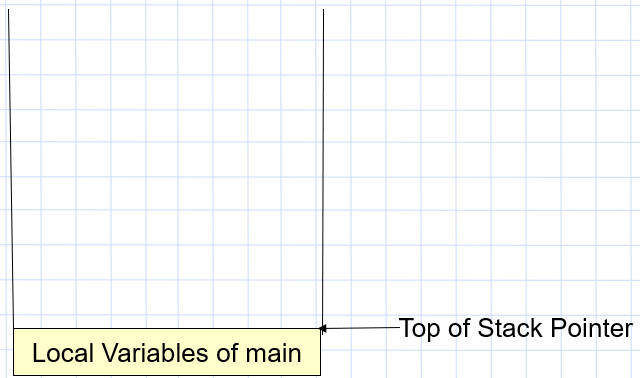
\includegraphics[width=0.8\textwidth]{images/memory_layout.png}
    \caption{Memory Layout of a Program}
    \label{fig:memory_layout}
\end{figure}

The stack pointer initially points to the top of the stack, which holds the local variables of the \texttt{main()} function. The stack grows downward (towards lower memory addresses), and this region of memory is used to manage function calls and their associated data.

Now suppose the \texttt{main()} function makes a call to another function, say \texttt{func1()}. In that case, the system allocates additional space on the stack for the function call. This includes space for:
\begin{itemize}
    \item The return address (i.e., the point in \texttt{main()} to resume execution after \texttt{func1()} finishes),
    \item Any arguments passed to \texttt{func1()},
    \item The local variables declared inside \texttt{func1()}.
\end{itemize}

This updated stack state is illustrated in Figure~\ref{fig:memory_layout_func1}. The stack pointer is now moved to point to the new top of the stack, corresponding to the local variables of \texttt{func1()}.

\begin{figure}[ht]
    \centering
    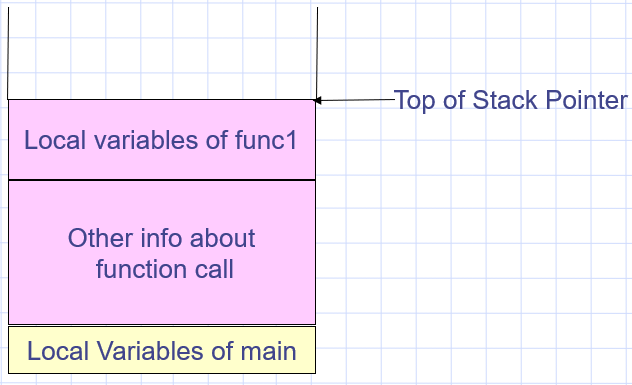
\includegraphics[width=0.8\textwidth]{images/memory_layout_func1.png}
    \caption{Memory Layout after a Function Call to \texttt{func1()}}
    \label{fig:memory_layout_func1}
\end{figure}

When \texttt{func1()} completes its execution and returns, the stack frame associated with it is deallocated. This involves:
\begin{itemize}
    \item Removing the local variables of \texttt{func1()},
    \item Restoring the return address,
    \item Adjusting the stack pointer back to its state before the call.
\end{itemize}

As a result, the stack pointer once again points to the top of the stack containing the local variables of \texttt{main()}, restoring the memory layout to its original state shown in Figure~\ref{fig:memory_layout}.
This mechanism of pushing function call data onto the stack and popping it off during function return is fundamental to how most programming languages, including C, manage nested and recursive function calls. It also underpins the concept of function call stacks and stack-based memory management.

\subsection{Program and Data}

When a program is compiled and executed, its memory layout is broadly divided into several segments, each serving a specific purpose. These include the code segment, data segments (initialized and uninitialized), heap, and stack.

The code is stored in the \textbf{text segment}, which contains the compiled machine instructions of the program. This segment is typically read-only and does not change during execution.

The \textbf{data segment} holds global and static variables. It is further divided into:
\begin{itemize}
    \item \textbf{Initialized Data Segment:} Contains global and static variables that are initialized by the programmer.
    \item \textbf{Uninitialized Data Segment (also called BSS):} Contains global and static variables that are declared but not explicitly initialized.
\end{itemize}
Both the code and data segments are fixed in size once the program starts running.

In contrast, two other regions of memory — the \textbf{heap} and the \textbf{stack} — are dynamic in nature:
\begin{itemize}
    \item The \textbf{heap} is used for dynamically allocated memory (e.g., using \texttt{malloc()} in C). The heap grows upwards as new memory is allocated during program execution.
    \item The \textbf{stack} is used for function call information, such as local variables, parameters, and return addresses. It grows downwards and shrinks as functions are called and returned.
\end{itemize}

This division and organization of memory during program execution is beautifully depicted in Figure~\ref{fig:program_data}.

\begin{figure}[ht]
    \centering
    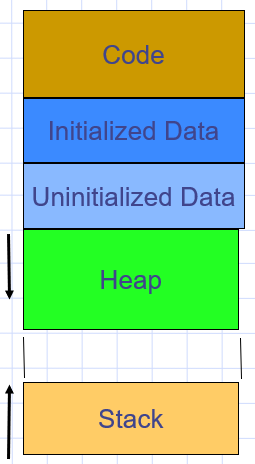
\includegraphics[width=0.25\textwidth]{images/program_data.png}
    \caption{Program and Data Memory Layout}
    \label{fig:program_data}
\end{figure}
A program utilizes the main memory in a structured way, with different sections allocated for different types of data and instructions. 

For instance, an instruction such as \texttt{add x, y, z} would be stored in the \textbf{text segment} (also referred to as the code segment) of the memory. This segment contains the compiled machine instructions that the CPU executes. It is typically read-only to prevent accidental overwriting of program instructions during execution.

The variables used in a program, on the other hand, are allocated in different memory segments depending on their lifetime and declaration style:

\begin{itemize}
    \item An integer variable like \texttt{int x}, if declared within a function, is likely to be \textbf{stack-allocated}. This means that memory for \texttt{x} is reserved on the call stack, and its lifetime is limited to the duration of the function's execution.
    
    \item A variable like \texttt{double w}, if allocated dynamically using functions such as \texttt{malloc()} or \texttt{calloc()}, is stored in the \textbf{heap segment}. The programmer must manage the lifetime of such variables explicitly using memory allocation and deallocation functions.
    
    \item A variable such as \texttt{float t}, if declared globally or as a static local variable, is stored in the \textbf{data segment}. This data segment can be further divided into:
    \begin{itemize}
        \item The \textbf{initialized data segment}, where variables with an explicit initial value reside.
        \item The \textbf{uninitialized data segment} (often called the BSS segment), which holds variables declared but not explicitly initialized.
    \end{itemize}
\end{itemize}

This organization of memory usage is depicted in Figure~\ref{fig:program_memory}.

\begin{figure}[ht]
    \centering
    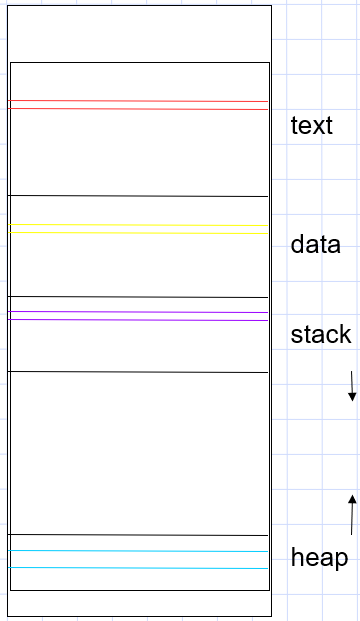
\includegraphics[width=0.5\textwidth]{images/program_memory.png}
    \caption{Program Memory Layout}
    \label{fig:program_memory}
\end{figure}


\section{Basic Computer Organization}

A computer system is broadly organized into three major components, as illustrated in Figure~\ref{fig:computer_organization}:

\begin{itemize}
    \item \textbf{Central Processing Unit (CPU) or Processor:} Often referred to as the brain of the computer, the CPU is responsible for executing instructions and performing all arithmetic and logical operations.
    
    \item \textbf{Main Memory:} This component is used to store both data and instructions temporarily during program execution. Memory is essential for the CPU to retrieve and process data efficiently.
    
    \item \textbf{Input/Output Devices (I/O Devices):} These devices enable the computer to interact with the external environment. Examples include keyboards, mice, monitors, and printers. Input devices send data to the computer, while output devices display or produce results.
\end{itemize}

\begin{figure}[H]
    \centering
    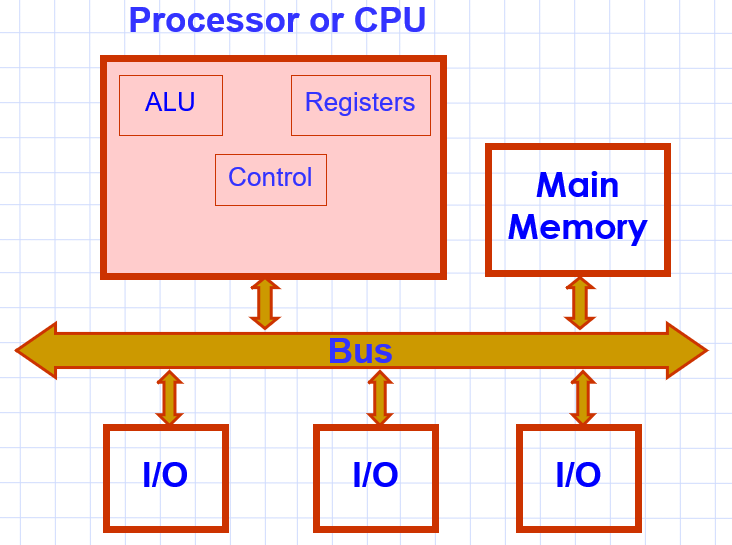
\includegraphics[width=0.5\textwidth]{images/computer_organization.png}
    \caption{Basic Computer Organization}
    \label{fig:computer_organization}
\end{figure}

The CPU itself is further divided into the following core components:

\begin{itemize}
    \item \textbf{Control Unit (CU):} The control unit manages and coordinates the operations of the CPU. It directs how data moves between the CPU, memory, and I/O devices. It decodes instructions and ensures that the correct sequence of operations is followed.

    \item \textbf{Arithmetic Logic Unit (ALU):} This unit performs all arithmetic operations (like addition, subtraction) and logical operations (like AND, OR, NOT). It acts as the computational engine of the CPU.

    \item \textbf{Registers:} Registers are small, high-speed storage locations built directly into the CPU. They hold temporary data and intermediate results while instructions are being executed. Registers play a key role in speeding up the processing as accessing them is significantly faster than accessing main memory.
    
    Registers are generally classified into two categories:
    \begin{itemize}
        \item \textbf{General Purpose Registers (GPRs):} These registers are available to the programmer for storing temporary values, such as operands or intermediate results. They help in reducing memory accesses. However, CPUs typically have a limited number of GPRs. One reason for using them is that there exists a large speed disparity between the CPU and main memory. For example:
        \begin{itemize}
            \item CPU operates at around 2 GHz, which corresponds to about 0.5 nanoseconds per cycle.
            \item Main memory accesses typically take 50--100 nanoseconds.
        \end{itemize}
        Because of this gap, using registers instead of repeatedly accessing memory helps improve performance.

        \item \textbf{Special Purpose Registers (SPRs):} These are reserved for specific control functions within the CPU. An important example is the \textbf{Program Counter (PC)}, which holds the address of the next instruction to be executed. Other SPRs may include status registers, instruction registers, and stack pointers depending on the architecture.
    \end{itemize}
\end{itemize}

\subsection{Main Memory and its problems}

One of the primary performance bottlenecks in modern computer systems arises due to the significant speed gap between the CPU and the main memory. While CPUs operate at very high frequencies (in the order of gigahertz), main memory (typically DRAM) is much slower—approximately $100\times$ slower. As a result, even though the CPU is capable of executing instructions rapidly, it often ends up idling while waiting for data to be fetched from the main memory.

Another related limitation is the scarcity of CPU registers. These registers are extremely fast and are used to store immediate data required for computations. However, their number is very limited, which means most data must be retrieved from main memory, further aggravating the memory bottleneck.

\begin{example}
    Let's consider a toy example to understand the main memory organization where the main memory has a size of 128 Bytes, and it is divided into blocks of size 4 Bytes. Since the memory is byte-addressable, each of the 128 Bytes has a unique memory address. To uniquely represent each of these 128 addresses, we require:
    \[
    \log_2 128 = 7 \text{ bits}
    \]
    Hence, memory addresses will range from $0000000_2$ to $1111111_2$. 

    The total number of memory blocks is:
    \[
    \frac{128}{4} = 32 \text{ blocks}
    \]
    
    Thus the number of bits that are used to identify the block number (since there are 32 blocks):
    \[
    \log_2 32 = 5 \text{ bits}
    \]

    Each block contains 4 Bytes, which requires 2 bits to specify the offset within the block:
    \[
    \log_2 4 = 2 \text{ bits}
    \]
    
    Therefore, any 7-bit memory address can be broken down into:
    \[
    \underbrace{b_6b_5b_4b_3b_2}_{\text{Block address (5 bits)}} \underbrace{b_1b_0}_{\text{Offset (2 bits)}}
    \]
    \begin{itemize}
        \item \textbf{Block address (5 bits):} Specifies which of the 32 blocks contains the address.
        \item \textbf{Offset (2 bits):} Specifies which byte within the block is being addressed.
    \end{itemize}

    This layout allows the system to efficiently locate a specific byte in memory by first identifying the block and then using the offset to access the byte within that block as shown in figure~\ref{fig:memory_addressing}.
    \begin{figure}[H]
        \centering
        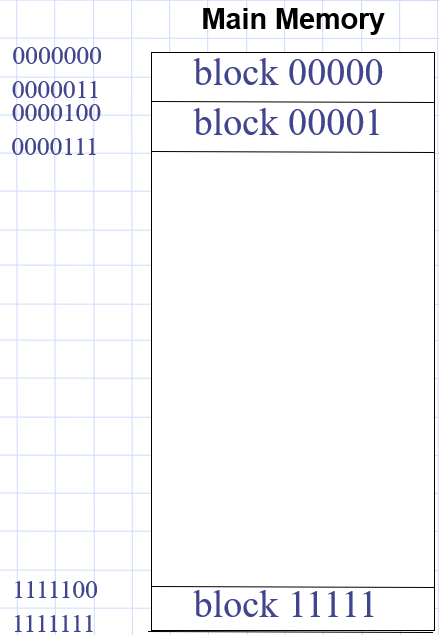
\includegraphics[width=0.5\textwidth]{images/memory_addressing.png}
        \caption{Memory Address Breakdown}
        \label{fig:memory_addressing}
    \end{figure}
\end{example}

\subsection{Cache Memory and Locality of Reference}
\textbf{The solution to this problem is the introduction of cache memory.} Cache is a small, high-speed memory that resides very close to or within the CPU itself. It acts as a buffer between the CPU and the main memory, storing frequently accessed data and instructions. If the data the CPU needs is found in the cache (called a \textit{cache hit}), it can be accessed much more quickly than from main memory. Otherwise, a \textit{cache miss} results in fetching data from the slower main memory.

The design of cache memory relies heavily on the \textbf{principle of locality of reference}, which exploits patterns in how programs access memory. There are two major types of locality:

\begin{itemize}
    \item \textbf{Temporal Locality:} This principle states that memory locations that have been accessed recently are least likely to be accessed again in the near future. For example, if a program accesses a variable, it is likely to access the same variable again soon. This is often seen in loops or repeated function calls where the same data is used multiple times.
    
    \item \textbf{Spatial Locality:} This principle states that memory locations near those that have been recently accessed are likely to be accessed soon. For instance, when iterating over an array, accessing one element implies that its neighboring elements will be accessed shortly.
\end{itemize}

By leveraging these two types of locality, cache memory significantly reduces the average memory access time and helps ensure that the CPU is not left waiting idly for data.


\section{Cache Composition}

Main memory is much larger than the cache. Hence, it is not possible to keep the entire memory content in the cache at once. So, when the CPU accesses a memory location, a portion of the memory which is a \textbf{memory block} is temporarily copied into the cache.

When the CPU needs to access a data item or an instruction, it refers to a specific memory address.
A memory address is divided into three fields:
\begin{itemize}
    \item \textbf{Tag:} Used to uniquely identify a block of memory among many possible candidates that could reside in the same cache set.
    \item \textbf{Index:} Identifies the specific cache set to which the memory block maps.
    \item \textbf{Offset:} Specifies the exact word or byte within the block.
\end{itemize}
It's schematic is as shown in the figure~\ref{fig:memory_address} .
\begin{figure}[H]
    \centering
    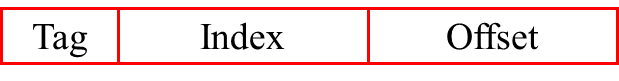
\includegraphics[width=0.5\textwidth]{images/memory_address.png}
    \caption{Memory Address Breakdown}
    \label{fig:memory_address}
\end{figure}
A cache can be broadly divided into two parts -cache directory which keep track of the address and information about whether the data is valid or not and the cache ram which actually stores the data. The cache is composed of multiple \textbf{sets}, where each set contains one or more \textbf{cache lines} (also called \textit{slots}). A cache line typically includes the following components:
\begin{itemize}
    \item \textbf{Tag:} A portion of the memory address used to verify if the data stored in the cache line corresponds to the requested address.
    \item \textbf{Valid Bit:} Indicates whether the data in the cache line is valid (i.e., whether it contains up-to-date information from main memory).
    \item \textbf{Data Block:} The actual data fetched from main memory.
\end{itemize}
It's schematic is as shown in the figure~\ref{fig:cache_memory}
\begin{figure}[H]
    \centering
    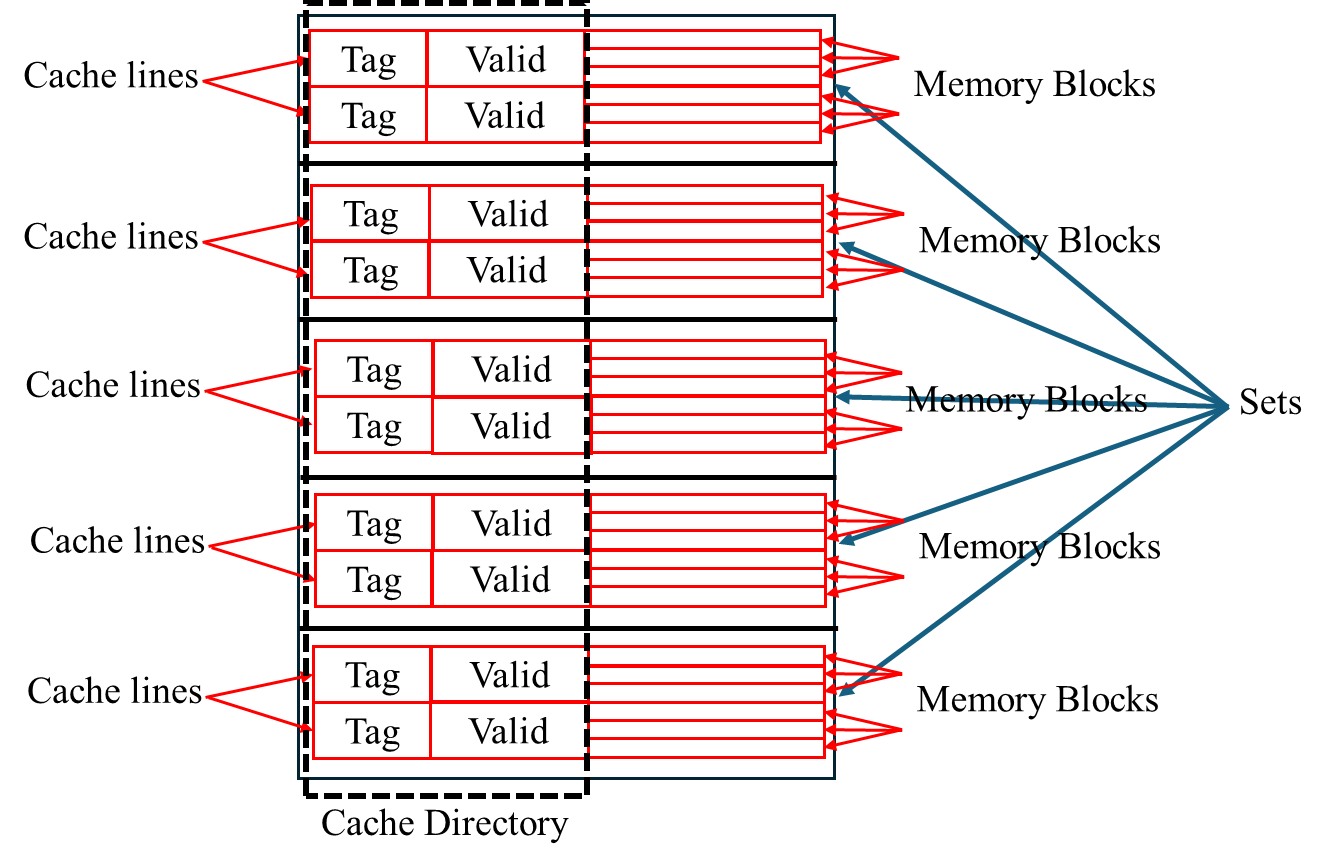
\includegraphics[width=0.8\textwidth]{images/cache_memory.png}
    \caption{Cache Memory}
    \label{fig:cache_memory}
\end{figure}

Main memory is organized into blocks or words, and cache memory is used to store a subset of these blocks for faster access. The cache is divided into small storage units called \textbf{cache lines} (or slots). Each cache line can hold exactly one block of data from the main memory. The process of deciding which cache line should hold which memory block is called \textbf{mapping}. Thus, ``mapping" refers to the rule that assigns a memory block to a particular cache line based on the memory address.

When a memory access occurs, the cache operates as follows:
\begin{enumerate}
    \item The \textbf{index} field is used to locate the appropriate cache set.
    \item Within the identified set, each cache line's tag is compared to the \textbf{tag} field of the memory address.
    \item If the tag matches and the \textbf{valid bit} is set, it results in a \textbf{cache hit}, and the data is fetched using the offset.
    \item If the tag does not match any line in the set, it results in a \textbf{cache miss}, and the data must be fetched from main memory.
\end{enumerate}
This is as illustrated in figure~\ref{fig:cache_lookup}
\begin{figure}
    \centering
    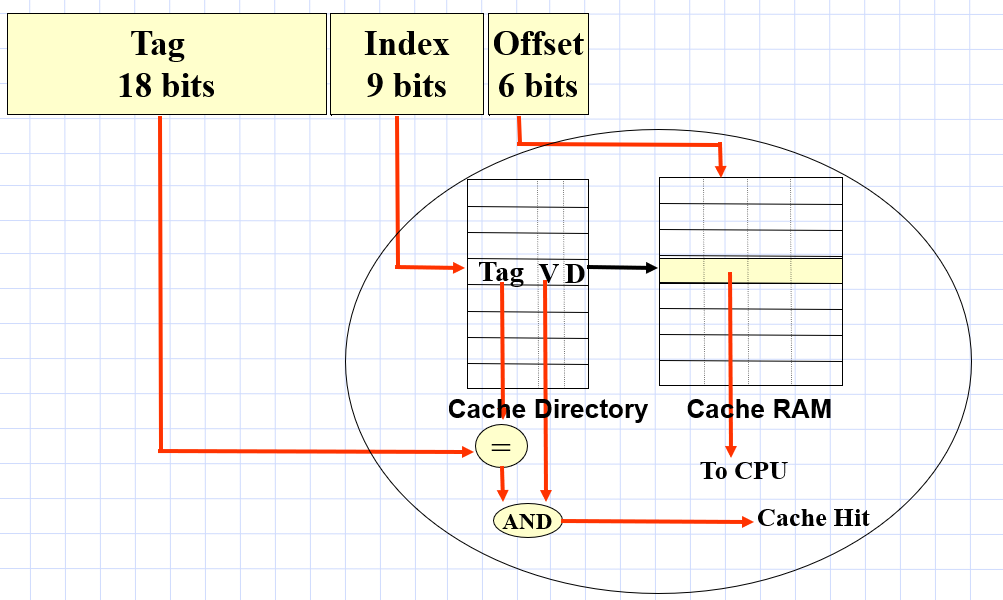
\includegraphics[width=0.7\linewidth]{images/mem_access.png}
    \caption{Cache Lookup and Access}
    \label{fig:cache_lookup}
\end{figure}
\begin{example}
Suppose a memory address is 16 bits long and the cache has 64 lines. Then, we need $\log_2 64 = 6$ bits to index the cache lines. These 6 bits are extracted from the memory address and used to determine which cache line the block maps to. So, memory blocks whose addresses share the same 6 index bits will always map to the same cache line.
\end{example}

The structure and number of sets and lines determine the type of cache organization (e.g., direct-mapped, set-associative, or fully associative, or even $m$-way set-associative), which will be discussed in subsequent sections.

\subsection{Direct-Mapped Cache}
In a \textbf{direct-mapped cache}, each cache set contains exactly \textbf{one cache line}. 


\subsubsection*{Cache Access Mechanism}
When the processor needs to access a memory word (instruction or data), it sends the corresponding memory address to the cache. The following steps occur:

\begin{enumerate}
    \item \textbf{Indexing:} The index bits of the memory address are used to determine the set (or cache line, in the case of direct-mapped cache) where the memory block might reside. This can be done very fast since the index bits refer to an address which can be located very easily.
    
    \item \textbf{Tag Comparison:} The remaining significant bits bits of the memory address, called the \emph{tag}, are compared with the tag stored in the selected cache line. Since there is only one cache line in each set, the index bits map to the cache lines directly.
    
    \item \textbf{Valid Bit Check:} Along with the tag, each cache line stores a valid bit indicating whether the data in the cache line is meaningful. If the valid bit is set and the tags match, a \textbf{cache hit} occurs.
    
    \item \textbf{Cache Hit:} If there is a match and the valid bit is set, the data is fetched directly from the cache, which is very fast compared to main memory access.
    
    \item \textbf{Cache Miss:} If the valid bit is not set or the tags do not match, a \textbf{cache miss} occurs. In this case:
    \begin{itemize}
        \item The processor fetches the required memory block from the main memory.
        \item In direct-mapped cache since each cache set contains exactly one cache line. This means that every memory block can map to exactly \emph{one} cache line in the cache. The specific line is determined using the \emph{index bits} of the memory address. These index bits identify which cache set the memory block corresponds to. Thus, a given memory block from main memory always maps to a single fixed location in the cache. If two memory blocks happen to have the same index bits, they will compete for the same cache line. When one is loaded, the other is evicted. This situation is known as a \textbf{conflict miss} and is a known limitation of direct-mapped caches. Thus, the fetched block is stored in the cache line corresponding to the index, replacing the existing block if any.
        \item The tag and valid bit of the cache line are updated.
        \item The processor resumes execution with the now-available data.
    \end{itemize}
    
\end{enumerate}

\paragraph{Advantages of Direct-Mapped Cache:}
\begin{itemize}
    \item Very simple to implement in hardware.
    \item Fast lookup due to one-to-one mapping.
    \item Less hardware cost compared to other mapping schemes.
\end{itemize}

\paragraph{Disadvantages of Direct-Mapped Cache:}
\begin{itemize}
    \item High chance of conflict misses. Two memory blocks in main memory that map to the same cache line will replace each other frequently.
    \item Poor utilization of cache space if many blocks compete for the same line.
\end{itemize}

Direct-mapped caches are efficient and fast, but the rigid mapping can lead to performance issues if many memory blocks map to the same cache line.

\subsection{Fully Associative Cache}
\label{sec:fully-associative-cache}

In a \textbf{fully associative cache}, any memory block can be stored in any cache line. It can be thought as only one cache set having all the cache lines. There is no fixed mapping between memory addresses and cache lines. So, there are no index bits in the address.

\subsubsection*{Cache Access Mechanism}
When the processor needs to access a data word or an instruction, it sends the memory address to the cache. The cache performs the following steps:

\begin{enumerate}
    \item \textbf{Tag Comparison – Associative Search:}  
    The memory address is divided into two parts: the \textbf{tag} and the \textbf{block offset}. Since any block can go into any cache line, there is no need for index bits.  
    The cache controller compares the tag of the incoming address with the tags of all cache lines in parallel. This is called an \textit{associative search}.

    \item \textbf{Valid Bit Check:}  
    Each cache line has a valid bit. It tells whether the content of the cache line is meaningful.  
    If the valid bit is set and the tag matches, we have a \textit{cache hit}.

    \item \textbf{Cache Hit:}  
    If there is a tag match and the valid bit is set, the required data is present in the cache. The data is directly sent to the processor. This access is much faster than going to the main memory.

    \item \textbf{Cache Miss:}  
    If there is no matching tag or the valid bit is not set, it results in a \textit{cache miss}. In this case:
    \begin{itemize}
        \item The required memory block is fetched from the main memory.
        \item The block is then placed into an available cache line.
        \item If all lines are full, one of the existing blocks is replaced using a \textit{replacement policy}. Common policies include:
        \begin{itemize}
            \item \textbf{FIFO (First-In-First-Out)}: Replace the oldest block.
            \item \textbf{LRU (Least Recently Used)}: Replace the block that was not used for the longest time.
            \item \textbf{Random}: Replace a randomly chosen block.
        \end{itemize}
        \item The tag and valid bit of the chosen cache line are updated.
        \item The processor resumes execution using the newly fetched data.
    \end{itemize}
\end{enumerate}

\subsubsection*{Advantages of Fully Associative Cache}
\begin{itemize}
    \item Very flexible. Any memory block can go into any cache line.
    \item Conflict misses are minimized, as blocks are not restricted to a fixed location.
\end{itemize}

\subsubsection*{Disadvantages of Fully Associative Cache}
\begin{itemize}
    \item Hardware is more complex. The cache must compare the incoming tag with all tags in parallel.
    \item Associative search uses more power and is slower than simple indexing.
    \item Cache access time is usually longer compared to a direct-mapped cache.
\end{itemize}



\subsection{Set Associative Cache}
\label{sec:set-associative-cache}

Set associative mapping is a hybrid between direct-mapped and fully associative caches. In this approach, the cache is divided into multiple \textbf{sets}. A $m$-way set associative means each set contains $m(>1)$ number of cache lines, also called \textit{ways}. A block of main memory maps to exactly one set, but it can go into any line within that set.

For example, consider a 4-way set-associative cache with 128 total cache lines. This means we have:
\[
\frac{128}{4} = 32 \text{ sets}
\]
Each set has 4 lines. A memory block is first mapped to a set using a portion of its address — typically using a modulo operation as shown in the figure~\ref{fig:set_associative} for a 2-way set-associative. Then, the block can be stored in any of the 4 lines within that set.

\begin{figure}[H]
    \centering
    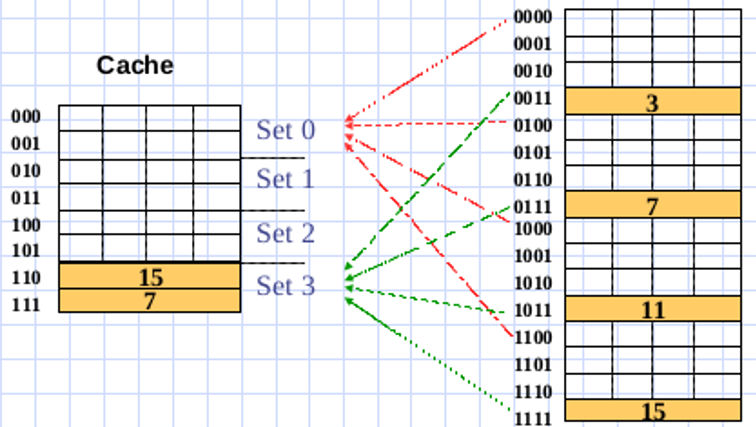
\includegraphics[width=0.5\linewidth]{images/set_associative.png}
    \caption{Set Associative Mapping}
    \label{fig:set_associative}
\end{figure}

\subsubsection*{Cache Access Mechanism}

When the processor needs to access a data word or an instruction, it sends the memory address to the cache. The following steps occur:

\begin{enumerate}
    \item \textbf{Indexing:}  
    The index bits from the memory address determine which set to look into. This is a fast and simple operation. It is similar to the indexing used in direct-mapped caches.

    \item \textbf{Tag Comparison (Associative Search within Set):}  
    The remaining significant bits of the address form the \textbf{tag}. The cache controller compares this tag with the tags of all cache lines inside the selected set. All lines in the set are checked in parallel.

    \item \textbf{Valid Bit Check:}  
    Each line in the set stores a valid bit. If the valid bit is set and the tag matches, the cache reports a \textbf{hit}.

    \item \textbf{Cache Hit:}  
    If a match is found, the data is fetched directly from the cache. This is much faster than accessing the main memory.

    \item \textbf{Cache Miss:}  
    If no matching tag is found or the valid bit is not set, a \textbf{miss} occurs. In that case:
    \begin{itemize}
        \item The memory block is fetched from the main memory.
        \item The block is placed into the corresponding set.
        \item If there is space (a line with invalid bit), the block is placed there.
        \item If all lines are occupied, one block is replaced using a replacement policy like:
        \begin{itemize}
            \item \textbf{FIFO (First-In-First-Out)}: Replace the oldest block.
            \item \textbf{LRU (Least Recently Used)}: Replace the least recently accessed block.
            \item \textbf{Random}: Replace a randomly chosen block.
        \end{itemize}
        \item The tag and valid bit are updated, and the processor resumes using the fetched data.
    \end{itemize}
\end{enumerate}
\begin{figure}[ht]
    \centering
    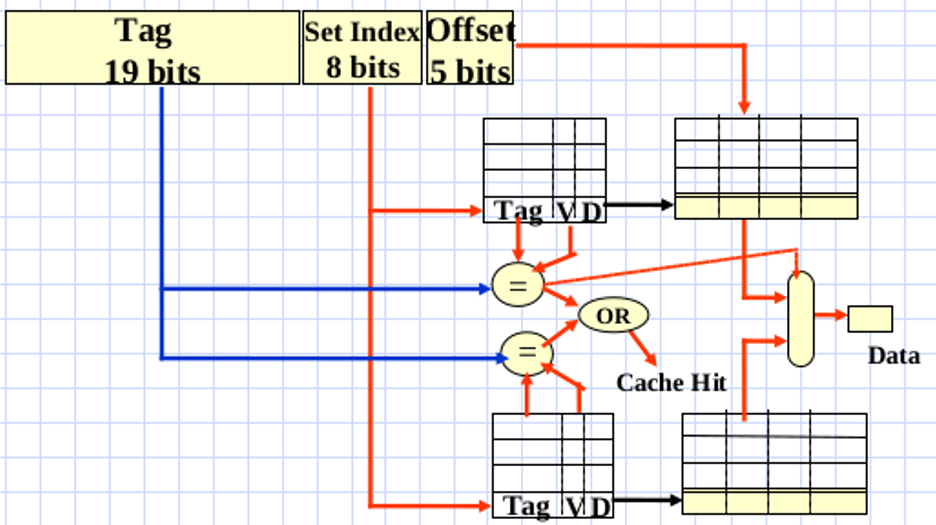
\includegraphics[width=0.7\linewidth]{images/2way_set.png}
\end{figure}
\subsubsection*{Advantages}
\begin{itemize}
    \item Reduces conflict misses compared to direct-mapped caches.
    \item More flexible than direct-mapped, but less complex than fully associative.
    \item Provides a good balance between speed, flexibility, and hardware cost.
\end{itemize}

\subsubsection*{Disadvantages}
\begin{itemize}
    \item Slightly slower than direct-mapped due to the parallel tag comparisons within each set.
    \item Requires more complex hardware than direct-mapped caches.
    \item Needs a replacement policy to decide which block to evict on a miss.
\end{itemize}

\begin{example}
Consider an example of an $8$ GB main memory (RAM). Let the size of each memory block be $64$ bytes and consider a typical cache size of $64$ KB, and assume a \textbf{2-way set-associative} mapping.

Since $8$ GB $\approx 2^{33}$ bytes, we need $33$ bits to uniquely identify each byte in memory (because $\log_2 2^{33} = 33$). Since the size of each memory block is $2^{64}$ bytes, which is $2^6$ bytes. Therefore, the total number of memory blocks in main memory is:
\[
    \frac{2^{33}}{2^6} = 2^{27}
\]
So, there are approximately $125 \times 10^6$ memory blocks.

To address these blocks, we need $27$ bits (since $\log_2 2^{27} = 27$). The remaining $6$ bits are used to specify the offset (i.e., the byte position) within a block.

Thus, each $33$-bit memory address can be divided as follows:
\begin{itemize}
    \item $27$ bits for the \textbf{block number}
    \item $6$ bits for the \textbf{offset} within the block
\end{itemize}

Since each memory block is $64$ bytes, each cache block is also $64$ bytes. In a 2-way set-associative cache, each \textbf{set} contains 2 blocks, meaning each set occupies $2 \times 64 = 128$ bytes.

So, the total number of sets in the cache is:
\[
    \frac{64 \text{ KB}}{128 \text{ bytes}} = \frac{2^{16}}{2^7} = 2^9 = 512 \text{ sets}
\]
Hence, we require $\log_2 512 = 9$ bits to index the cache sets.

Now recall that we need $27$ bits to address a memory block (from earlier). In set-associative mapping, the \textbf{least significant} $9$ bits of the block number are used as the \textbf{index} into the cache. The \textbf{remaining} $18$ bits serve as the \textbf{tag}, which is stored in the tag directory to check if a block is present in a set.

Finally, we still need the $6$ offset bits to identify the specific byte within the block.

Therefore, the 33-bit memory address is divided into:
\begin{itemize}
    \item \textbf{18 tag bits} (for block identification)
    \item \textbf{9 index bits} (for set selection)
    \item \textbf{6 offset bits} (for byte within block)
\end{itemize}

When the processor wants to access some data or an instruction, it sends a 33-bit memory address. This address is first searched in the cache. This also depends on the type of mapping associated with cache.

Since we are using a 2-way set associative cache, each cache set has 2 cache lines. The cache uses some bits of the memory address sent by the processor (called \textbf{index bits}) to find the correct set. Once the set is located, the cache compares the \textbf{tag bits} of the address with the tags stored in the two cache lines of that set. If there is a match, and the \textbf{valid bit} is set, it is a \textbf{cache hit}. This means the data is already in the cache and is sent to the processor. If there is no match, or the valid bit is not set, it is a \textbf{cache miss}. The data must then be fetched from the main memory and placed into one of the cache lines in that set.

In the case of a \textbf{cache miss}, the data or instruction requested by the processor must be fetched from the main memory and placed into the cache. Since the size of cache memory is limited, an existing memory block currently in the cache must be evicted to make room for the newly fetched block. The strategy used to determine which cache line gets replaced is called the \textbf{cache replacement policy}. In an $2$-way \textbf{set-associative cache}, the memory block is mapped to a cache set based on the index bits, and it can replace any of the $2$ cache lines within that set. Again, policies like FIFO or LRU are used to decide which of the $2$ lines in the set will be evicted and replaced by the new block. This design offers a trade-off between the high flexibility of a fully associative cache and the simple implementation of a direct-mapped cache.
\end{example}

\begin{example}
The table below gives the parameters for a number of different caches. For each cache, determine $S$, $t$, $s$, and $b$.

\begin{center}
\begin{tabular}{|c|c|c|c|c|c|c|c|c|}
    \hline
    Cache & $m$ & $C$ & $B$ & $E$ & $S$ & $t$ & $s$ & $b$ \\
    \hline
    1 & 32 & 1024 & 4  & 256 & \textcolor{blue}{1}  & \textcolor{blue}{30} & \textcolor{blue}{0} & \textcolor{blue}{2} \\
    \hline
    2 & 32 & 1024 & 8  & 128 & \textcolor{blue}{1}  & \textcolor{blue}{29} & \textcolor{blue}{0} & \textcolor{blue}{3} \\
    \hline
    3 & 32 & 1024 & 32 & 32  & \textcolor{blue}{1}  & \textcolor{blue}{27} & \textcolor{blue}{0} & \textcolor{blue}{5} \\
    \hline
    4 & 32 & 1024 & 32 & 2   & \textcolor{blue}{16} & \textcolor{blue}{23} & \textcolor{blue}{4} & \textcolor{blue}{5} \\
    \hline
\end{tabular}
\end{center}

\vspace{1em}
\textbf{Explanation for Cache 1:}

Given:
\begin{itemize}
    \item $m = 32$, $C = 1024$ bytes, $B = 4$ bytes, $E = 256$
\end{itemize}

Then:
\begin{itemize}
    \item Total blocks $= \frac{C}{B} = \frac{1024}{4} = 256$
    \item Number of sets $S = \frac{C}{B\cdot E} = \frac{256}{256} = 1$
    \item Block offset bits $b = \log_2 B = \log_2 4 = 2$
    \item Set index bits $s = \log_2 S = \log_2 1 = 0$
    \item Tag bits $t = m - s - b = 32 - 0 - 2 = 30$
\end{itemize}

The same formulas can be used for the other entries.
\end{example}


\begin{note}
    Note that in this section, we have not gone into the nitty-gritty details of how cache works internally or how it is managed by the system. We have skipped several important topics such as write strategies (like write-through and write-back), cache coherence in multi-core systems, and the structure of real-world cache hierarchies (like L1, L2, and L3 caches). Our goal here was to give a high-level understanding of what a cache is and how it helps speed up memory access. We will revisit some of these advanced topics later in the book if needed. For a deeper explanation, refer to the book~\cite{bryant2016computer}.
\end{note}

\section{Cache and Programming}
In this section, we will learn how cache-related performance issues can affect important parts of our programs. We will also look at some simple examples to understand this better. 

For simplicity, we will focus only on the \textbf{data cache}, assuming that instruction and data caches are separate. Let the memory address be of $32$ bits. The configuration of the data cache we will be working with is as follows:
\begin{itemize}
    \item Cache type: Direct-mapped
    \item Cache size: 16 KB
    \item Block size: 32 Bytes
\end{itemize}

Since the cache is direct-mapped with a total size of 16 KB and a block size of 32 Bytes, it contains:
\begin{itemize}
    \item $\frac{16 \times 1024}{32} = 512$ cache lines (or sets because of direct-mapped cache)
    \item Thus, $\log_2 512 = 9$ index bits,
    \item and $\log_2 32 = 5$ block offset bits
    \item The remaining $18$ bits will be the tag bits.
\end{itemize}
\subsection{Example 1: Vector Sum Reduction}

We are interested in computing a scalar value that reduces a vector by summing all its elements. This requires a loop that adds each element of the vector to an accumulator.

\begin{lstlisting}[style=cppstyle, caption={Vector Sum Reduction}]
double A[2048], sum = 0.0;
for (i = 0; i < 2048; i++) sum = sum + A[i];
\end{lstlisting}

In this example, the array \texttt{A} contains 2048 double-precision values, with each value occupying $8$ bytes (64-bit format). The variable \texttt{sum} is also of type \texttt{double}, and thus occupies $8$ bytes.

The loop iterates through all the elements of the array, adding each value of \texttt{A[i]} to the \texttt{sum} variable. This is a simple example of a vector reduction operation, often used in numerical computations.

To analyze cache behavior, we must examine the program at a level close to machine code to identify memory load and store operations. Specifically, we want to determine which memory accesses occur and in what order, given our data cache configuration—a direct-mapped 16KB cache with 32-byte block size.

For simplicity, we assume that the variables \texttt{i} and \texttt{sum} reside in registers. This is a reasonable assumption, as we can ensure that these variables are kept in registers by the compiler or through manual optimization. As a result, they do not involve memory accesses and therefore do not impact cache performance.

Hence, we will focus only on memory accesses to the array \texttt{A}, since it is the only data structure being read from memory in the loop. Therefore, analyzing the vector sum reduces to understanding what happens when accessing \texttt{A[0]}, \texttt{A[1]}, ..., up to \texttt{A[2047]}. We will now examine how this sequential access translates into memory operations:
\begin{itemize}
    \item Each element \texttt{A[i]} (for $i = 0$ to $2047$) must be loaded from memory into a CPU register. Here, a \textbf{load} refers to an instruction that copies data from main memory into a register. Once in a register, the value can be added to the \texttt{sum} variable.
    
    \item To proceed with the analysis, we assume that the base address of the array \texttt{A} (i.e., the address of \texttt{A[0]}) is \texttt{0xA000}, which corresponds to the binary address \texttt{10101000000000000}, with all more significant bits set to zero.
    
    \item Since our cache is 16KB (i.e., $2^{14}$ bytes) with a block size of 32 bytes (i.e., $2^5$), the cache is divided into $2^9 = 512$ blocks. So, we need 9 index bits and 5 offset bits. We’ll analyze cache behavior by tracking how these 14 bits (9 index + 5 offset) change as the array is accessed sequentially.
    
    \item The index bits for \texttt{A[0]} are \texttt{100000000} (which is decimal 256). So \texttt{A[0]} will map to cache index 256.
    
    \item Since the array elements are of type \texttt{double}, each occupies 8 bytes. A 32-byte block can thus hold 4 consecutive elements: \texttt{A[0]}, \texttt{A[1]}, \texttt{A[2]}, and \texttt{A[3]}.
    
    \item So, when there’s a cache miss for \texttt{A[0]}, the entire block containing \texttt{A[0]} through \texttt{A[3]} is brought into the cache. That means subsequent accesses to \texttt{A[1]}, \texttt{A[2]}, and \texttt{A[3]} will be cache hits.
    
    \item The next miss happens at \texttt{A[4]}, which maps to index 257. But again, a full block containing \texttt{A[4]} to \texttt{A[7]} is loaded. So \texttt{A[5]}, \texttt{A[6]}, and \texttt{A[7]} will hit in cache.
    
    \item This pattern continues — every 4th access is a miss (cold miss), and the next three accesses are hits due to spatial locality.
\end{itemize}

We now analyze this behavior assuming the cache is initially empty, which is also known as a \textbf{cold start}. The first access to each block (like \texttt{A[0]}, \texttt{A[4]}, \texttt{A[8]}, etc.) causes a cache miss, but the next three accesses within that block are cache hits. 

So, in total, there are $2048 / 4 = 512$ cache misses (one for every block of 4), and $2048 - 512 = 1536$ cache hits. This gives us a \textbf{hit ratio} of:
\[
\frac{1536}{2048} = 0.75 \quad \text{or} \quad 75\%
\]
This performance gain comes entirely from \textbf{spatial locality} — because we're accessing data laid out consecutively in memory.

Now suppose we add a loop before the reduction to preload all relevant memory blocks:
\begin{lstlisting}[style=cppstyle, caption={Preloading the Array for Temporal Locality}]
for (i = 0; i < 2048; i++) tmp = A[i]; // preload
double A[2048], sum = 0.0;
for (i = 0; i < 2048; i++) sum = sum + A[i];
\end{lstlisting}

With this change, the second loop sees a \textbf{100\% hit ratio}. This is because:
\begin{itemize}
    \item $75\%$ of hits come from \textbf{spatial locality} (within each block), and
    \item $25\%$ of hits come from \textbf{temporal locality}, since the data was already loaded in the first loop and hasn't been evicted.
\end{itemize}

Suppose now the array is defined as \texttt{double A[4096]}. Will this make any difference? Consider the case where the loop is preceded by another loop that accesses all array elements in sequential order. The total memory required to store the array is $8 \times 4096 = 32$~KB, while the cache memory is only 16~KB. Hence, the entire array cannot fit into the cache. After execution of the previous loop, the second half of the array will be in the cache and because of the spatial locality of reference it is anyways not going to be used for vector sum. This is just wasting time due to unnecessary memory accesses to no advantage. As a result, our loop will still experience cache misses, just as we analyzed earlier.

Recall that to estimate the data cache hit rate, we made the following assumptions:
\begin{itemize}
    \item The variables \texttt{sum} and \texttt{i} are stored in registers; hence, we ignore their memory accesses.
    \item The base address of \texttt{A[0]} is assumed to be \texttt{0xA000}.
    \item We consider that only load/store instructions access memory operands; all other instructions use register operands.
\end{itemize}

\subsection{Example 2: Vector Dot Product}
In this case, we are interested in computing the dot product (also called the inner product) between two vectors, $A$ and $B$, represented by the arrays \texttt{A} and \texttt{B}. The dot product is computed by taking the running sum of the products of corresponding elements from the two arrays. 

As in the previous example, we will assume similar conditions and ignore the accesses to the loop index variable \texttt{i} and the variable \texttt{sum}, assuming they are stored in registers. Also, we will assume that only load/store instructions access memory operands; all other instructions use register operands.

\begin{lstlisting}[style=cppstyle, caption={Vector Dot Product}]
double A[2048], B[2048], sum = 0.0;
for (i = 0; i < 2048; i++) 
    sum = sum + A[i] * B[i];
\end{lstlisting}

We are interested in analyzing the order of reference sequence, which will be: \texttt{load A[0]}, \texttt{load B[0]}, and so on, till \texttt{load A[2047]}, \texttt{load B[2047]}.

We now assume the base addresses of arrays $A$ and $B$ as $0xA000$ and $0xE000$ respectively. Since these arrays are declared as \texttt{double}, each element occupies $8$ bytes, and therefore, $4$ consecutive elements of the array will fit into each $32$-byte cache block.

Now, $0xA000$ in binary is $1010\ 0000\ 0000\ 0000$, which corresponds to cache index $256$. Similarly, $0xE000$ in binary is $1110\ 0000\ 0000\ 0000$, which also maps to the same index $256$.

Because the index bits are the same, both $A[0]$ and $B[0]$ will be loaded into the same cache set (index $256$). This leads to a problem: consider the load sequence. When we first load $A[0]$, there is a cache miss (a cold miss, assuming the cache is initially empty) at cache set index $256$. Thus, it loads $A[0] A[1], A[2], A[3]$ into the cache set memory block. Next, when we load $B[0]$, it maps to the same cache set index and causes another miss — this time a conflict miss, because it replaces the block holding $A[0]$.

A conflict miss occurs when multiple memory blocks map to the same cache set and compete for space under a direct-mapped cache scheme. In this case, since $A[0]$ and $B[0]$ conflict with each other, loading $B[0]$ causes memory block containing $A[0], A[1], A[2], A[3]$ to be evicted and load $B[0], B[1], B[2], B[3]$ into the cache set memory block. Now, when \texttt{load A[1]} is executed, it again maps to the same cache set (index $256$), and because it is not in the cache (recall the memory block containing $A[0], A[1], A[2], A[3]$ was evicted), we get yet another cache miss.

This process continues, resulting in a conflict miss for every access, significantly reducing cache efficiency. Thus, the hit ratio for our program is $0\%$. The source of the problem is that the elements of arrays $A$ and $B$ are accessed in order and both map to the same cache index. As a result, each new access causes the previous entry to be evicted, leading to no cache reuse. The hit ratio would have been better if the base address of array $A$ had been different from that of array $B$, such that the memory blocks mapped to different cache set indices. This would have prevented the conflicts and improved the cache performance.

The question now is: was this a contrived example? The root cause of the problem was that we assumed the base addresses of arrays $A$ and $B$ to be $0xA000$ and $0xE000$, respectively, such that both mapped to the same cache set index. Is this an unreasonable assumption that never occurs in the real world? The answer is no—it is not an unreasonable assumption. In fact, this behavior is consistent with the memory allocation model typically followed by compilers.

To understand this better, we must ask: how are variable addresses assigned by the compiler? Typically, the compiler begins allocating memory from a starting address, which is often outside the programmer’s control. Suppose, for instance, that the compiler begins by placing array $A$ at address $0xA000$. It then assigns memory to subsequent variables in the order they are declared. Since array $A$ consists of $2048$ elements of type \texttt{double} (each 8 bytes), the total space it occupies is $2048 \times 8 = 16384$ bytes, or $0x4000$ in hexadecimal. Therefore, array $B$ will be placed at address $0xA000 + 0x4000 = 0xE000$.

\[
\text{Address of } B = 0xA000 + 2048 \times 8 = 0xA000 + 0x4000 = 0xE000
\]
\[
\text{Binary: } 1010\ 0000\ 0000\ 0000 + 0100\ 0000\ 0000\ 0000 = 1110\ 0000\ 0000\ 0000
\]

Thus, both arrays may end up mapping to the same cache set index, causing conflict misses, even though this layout results naturally from how compilers assign addresses in practice.

Thus, the problem arises due to the nature of the cache hardware and the specific issue caused by the vector size of $2048$. The compiler typically assigns addresses to variables in the order they are declared.

Our objective is therefore to shift the base address of array $B$ just enough so that the cache index of $B[0]$ differs from that of $A[0]$:
\begin{lstlisting}[style=cppstyle]
double A[2052], B[2048];
\end{lstlisting}

Now, the base address of $B$ would be
\[
0xA000 + 2052 \times 8 = 0xE020,
\]
which corresponds to a cache index of $257$. Hence, $B[0]$ and $A[0]$ no longer conflict for the same cache block. The resulting hit ratio will rise to \textbf{75\%}. 

This is a common optimization trick used in languages like \textbf{Fortran}. By doing so, we have improved the cache hit ratio—but what impact does this have on the execution time of the program?

Suppose the following piece of code is a dominant part of the program, i.e., its performance heavily influences the overall execution time. Let us now analyze the number of cycles required for execution.

Assume there are $20$ machine instructions inside the loop: $2$ load instructions and $18$ others (such as additions, register loads, and loop overhead), which do not access memory and thus take only $1$ cycle per instruction. The total number of instructions executed is therefore $20 \times 2048$.

Assume each instruction takes $1$ cycle to execute, and a load miss incurs a penalty of $100$ cycles to fetch the data from memory.

\begin{itemize}
    \item \textbf{Best Case (100\% hit ratio):}  
    All instructions take only $1$ cycle. Thus, total cycles =  
    \[
    20 \times 2048 = 40960 \text{ cycles}.
    \]
    
    \item \textbf{Worst Case (0\% hit ratio):}  
    All $18$ non-load instructions take $1$ cycle each. The $2$ load instructions take $100$ cycles each due to cache misses. Thus, the total number of cycles is  
    \[
    (18 \times 1 + 2 \times 100) \times 2048 = (18 + 200) \times 2048 = 446464 \text{ cycles}.
    \]
    
    \item \textbf{Intermediate Case (75\% hit ratio):}  
    $75\%$ of the loads are cache hits (taking $1$ cycle), and $25\%$ are misses (taking $100$ cycles). So the load-related cycles are  
    \[
    0.75 \times 2048 \times 2 \times 1 + 0.25 \times 2048 \times 2 \times 100 = 3072 + 102400.
    \]
    The remaining $18$ instructions per iteration (which are not memory loads) always take $1$ cycle:  
    \[
    18 \times 2048 = 36864.
    \]
    Hence, the total number of cycles is  
    \[
    3072 + 102400 + 36864 = 142336 \text{ cycles}.
    \]
\end{itemize}

Thus, we observe that a better cache hit ratio significantly reduces the execution time—improving performance by almost a factor of $3$ compared to the $0\%$ hit case, and closing the gap toward the ideal case.


Another method is called \textbf{Array Merging}, where we merge the arrays $A$ and $B$ together, as shown in the following code:

\begin{lstlisting}[style=cppstyle]
struct {double A, B;} array[2048];
for (i = 0; i < 2048; i++) 
    sum += array[i].A * array[i].B;
\end{lstlisting}

The nature of the dot product remains the same, but now it picks two elements from the same array element of the newly defined structure. The idea is that spatial locality of reference will help here because the compiler will store \texttt{A[i]} and \texttt{B[i]} adjacent in memory since they are part of the same \texttt{struct}. 

Of course, in many programs, such a redefinition might not be possible, because \texttt{A} and \texttt{B} may have distinct meanings or uses in the calculations being performed, and it may not always be feasible to restructure the data in this way.

In this method, the hit ratio will again be $75\%$ because each cache block will now contain \texttt{A[0]}, \texttt{B[0]}, \texttt{A[1]}, \texttt{B[1]}, and so on. Thus, the first access to \texttt{A[0]} will be a cache miss due to a cold start, but the accesses to \texttt{B[0]}, \texttt{A[1]}, and \texttt{B[1]} will be cache hits.

\subsection{Example 3: DAXPY}

We now consider another famous example called DAXPY (\textbf{D}ouble precision \textbf{AX} \textbf{P}lus \textbf{Y}), where $a$ is a scalar and $X$ and $Y$ are vectors.

\begin{lstlisting}[style=cppstyle, caption={Double precision AX Plus Y (DAXPY)}]
double X[2048], Y[2048], a;
for (i = 0; i < 2048; i++) 
    Y[i] = a * X[i] + Y[i];
\end{lstlisting}

This example differs slightly from the previous one, as there are three array references per iteration of the loop. Specifically, for each $i$, we must load \texttt{X[i]}, load \texttt{Y[i]}, and then store the updated value back to \texttt{Y[i]}. 

The reference sequence thus becomes: 
\begin{center}
\texttt{load X[0], load Y[0], store Y[0], load X[1], load Y[1], store Y[1],} $\dots$, \texttt{load X[2047], load Y[2047], store Y[2047]}
\end{center}

Assuming that the base addresses of arrays \texttt{X} and \texttt{Y} do not conflict in the cache, we can compute the hit ratio. In this case, out of every 12 memory references (two loads and one store per iteration), there will typically be 1 miss for \texttt{X[0]} and 1 miss for \texttt{Y[0]} due to cold starts. The remaining references will be cache hits assuming spatial locality is exploited effectively. Thus, the overall hit ratio is approximately $\frac{10}{12}\times 100 =  83.3\%$.

\subsection{Example 4: 2D Matrix Sum}
We will now look at the sum of two-dimensional matrices as shown below:

\begin{lstlisting}[style=cppstyle]
double A[1024][1024], B[1024][1024];
for (j = 0; j < 1024; j++)
    for (i = 0; i < 1024; i++)
        B[i][j] = A[i][j] + B[i][j];
\end{lstlisting}

This is somewhat similar to DAXPY, and the reference memory access sequence would be:  
\texttt{load A[0,0], load B[0,0], store B[0,0], load A[1,0], load B[1,0], store B[1,0],} and so on.

Before analyzing the cache hit rate, it is important to answer a more fundamental question:  
\textbf{In what order are the elements of a multidimensional array stored in memory?}

In the case of one-dimensional arrays, the elements are stored contiguously in memory. However, when dealing with two-dimensional matrices, we must ask whether the matrix is stored row by row (row-major order) or column by column (column-major order). Different programming languages make different assumptions regarding this.

Compilers implement address calculations for multidimensional arrays based on the language's assumed storage order. Therefore, to compile a program correctly in terms of memory load and store operations, the compiler must know how the language stores multidimensional arrays. It is assumed that the compiler already knows the language-specific storage convention. Otherwise, it would have to make its own assumptions, which could severely affect performance portability.

\textbf{Performance portability} refers to the idea that even if a program remains functionally correct across different compilers or languages, its performance may vary significantly depending on how the underlying compiler interprets the array storage order.

This storage order convention is a property of the language, not the compiler. The two common conventions are:

\begin{itemize}
    \item \textbf{Row-major order:}
    \begin{itemize}
        \item For a two-dimensional array, the elements of the first row are stored first, followed by the elements of the second row, then the third, and so on.
        \item This is the convention used in \texttt{C}.
    \end{itemize}
    
    \item \textbf{Column-major order:}
    \begin{itemize}
        \item For a two-dimensional array, the elements are stored column by column in memory.
        \item This is the convention used in \texttt{Fortran}.
    \end{itemize}
\end{itemize}
Now, we are assuming the programming language to be C. In C, multi-dimensional arrays are stored in \textbf{row-major order}, which means that elements like $A[0][0]$, $A[0][1]$, $A[0][2]$, and $A[0][3]$ are stored in adjacent memory locations, typically mapping to the same cache block. Therefore, the given program is written inefficiently. 

To understand this, consider the reference sequence: if we access $A[1][0]$ immediately after $A[0][0]$, these elements are stored in different rows and thus different cache blocks, resulting in a cache miss. This indicates poor \textbf{spatial locality}.

We observe a mismatch between the \textbf{reference order}—the order in which memory is accessed—and the \textbf{storage order}—the way memory is actually laid out. Our program steps through the matrix column by column, resembling \textbf{column-major order}, whereas C stores matrices in \textbf{row-major order}: $A[0][0]$, $A[0][1]$, and so on. As a result, our loop does not exploit spatial locality, although it does demonstrate some \textbf{temporal locality}, since the store operation to $B[0][0]$ immediately follows a load from $B[0][0]$, which remains in the cache.

Thus, the loop will not show any spatial locality. Here, we assume that packing has been done to eliminate conflict misses due to base addresses. However, in this case, it does not really matter, as there is no spatial locality anyway, and temporal locality will not be affected by conflict misses. So we get:
\begin{itemize}
    \item A miss on \texttt{load A[0][0]} (due to cold start),
    \item A miss on \texttt{load B[0][0]} (due to cold start),
    \item A hit on \texttt{store B[0][0]} (due to temporal locality),
\end{itemize}
Now, when we go to the next instruction \texttt{load A[1][0]}, we again get a miss (due to cold start), and so on. Thus, the hit ratio is approximately $33\%$, entirely because of the temporal locality—on the store instructions. There are no hits for the load instructions at all.

Will \texttt{A[0][1]} be in the cache when required later in the loop? 

Now let us analyze the impact of \textbf{loop interchange}. Recall that in the initial version of the loop, the second subscript was in the outer loop and the first subscript was in the inner loop. We now consider the interchanged version, where the first subscript is in the outer loop and the second subscript is in the inner loop, as shown below:

\begin{lstlisting}[style=cppstyle]
double A[1024][1024], B[1024][1024];
for (i = 0; i < 1024; i++)
    for (j = 0; j < 1024; j++)
        B[i][j] = A[i][j] + B[i][j];
\end{lstlisting}

In this case, the memory reference sequence would be:
\begin{itemize}
    \item \texttt{load A[0][0]}, \texttt{load B[0][0]}, \texttt{store B[0][0]}
    \item \texttt{load A[0][1]}, \texttt{load B[0][1]}, \texttt{store B[0][1]}
    \item $\dots$
\end{itemize}

We observe that the first time \texttt{A[0][0]} is loaded, it results in a cache miss due to a cold start. Similarly, \texttt{load B[0][0]} will also result in a cache miss. However, the subsequent \texttt{store B[0][0]} will be a cache hit, since the value was just loaded and remains in the cache. Similarly, \texttt{load A[0][1]} will likely be a cache hit as it resides in the same cache block as \texttt{A[0][0]}, assuming a typical cache line size of 4 words. The same applies to the accesses for \texttt{B[0][1]}, \texttt{store B[0][1]}, and so on.

Hence, out of the first 12 memory instructions (8 loads and 4 stores), 10 will be cache hits and only 2 will be cache misses. This leads to a cache hit rate of:
\[
\frac{10}{12} \times 100 = 83.3\%
\]
This improved hit rate demonstrates better \textbf{spatial locality} due to the access pattern now matching the row-major storage layout of C arrays.

This leads to an important question: is it always safe to perform loop interchange? Consider the following example, where the secondary subscript is controlled by the outer loop:

\begin{lstlisting}[style=cppstyle]
for (j = 1; j < 2048; j++)
    for (i = 1; i < 2048; i++)
        A[i][j] = A[i+1][j-1] + A[i][j-1];
\end{lstlisting}

This ordering is clearly incorrect since the second subscript, which denotes the column (i.e., `j`), is controlled by the outer loop. We have already discussed such cases previously. This example is trivial, but many numerical codes still fall into this trap. We are interested in the version where the `for` loops are interchanged, since we know that doing so can improve spatial locality.

Let us examine the actual behavior of this loop by tracing its first few iterations. For instance:
\[
A[1][1] = A[2][0] + A[1][0], \quad A[2][1] = A[3][0] + A[2][0], \quad \text{and so on}.
\]
Then, for the next column:
\[
A[1][2] = A[2][1] + A[1][1].
\]

Now let us blindly interchange the two `for` loops and observe the effect:

\begin{lstlisting}[style=cppstyle]
for (int i = 1; i < 2048; i++)  // interchanged
    for (int j = 1; j < 2048; j++)
        A[i][j] = A[i+1][j-1] + A[i][j-1];
\end{lstlisting}


With this ordering, the first few iterations will now be:
\[
A[1][1] = A[2][0] + A[1][0], \quad A[1][2] = A[2][1] + A[1][1], \quad \text{and so on,}
\]
until we reach:
\[
A[2][1] = A[3][0] + A[2][0].
\]

Notice the subtle but crucial difference. In the original loop nest, the computation of $A[1][2]$ used updated values of both $A[2][1]$ and $A[1][1]$. However, in the interchanged version, the value of $A[1][2]$ is computed using the old value of $A[2][1]$ (since `i = 2` has not yet been processed) and the updated value of $A[1][1]$. This changes the computation semantics and may lead to incorrect results.

Hence, \textbf{loop interchange is not always safe}, especially when data dependencies exist across loop iterations. One must carefully analyze the dependencies before performing such optimizations.

Is there any safer way to modify the loops so that the code remains correct while also achieving better spatial locality? The answer is yes. This can be accomplished by rewriting the loop to iterate over the second subscript from higher to lower values, as shown below:

\begin{lstlisting}[style=cppstyle]
for (i = 2047; i > 1; i--)
    for (j = 1; j < 2048; j++)
        A[i][j] = A[i+1][j-1] + A[i][j-1];
\end{lstlisting}

This transformation ensures that data accessed in close temporal proximity is also stored in adjacent memory locations, thus taking better advantage of spatial locality.

However, this example also illustrates an important principle: \textbf{loop interchange should not be applied blindly}. Instead, the loop structure should be carefully analyzed or modified to exploit the memory hierarchy effectively. Such strategies can be learned through experience, systematic experimentation, or by exploring various loop arrangements and identifying those that provide the best spatial locality of reference.

\subsection{Example 5: Matrix Multiplication}
Here is an example for matrix multiplication.
\begin{lstlisting}[style=cppstyle]
double X[N][N], Y[N][N], Z[N][N];
for(i=0;i<N;i++)
    for (j=0lj<N;j++)
        for(k=0;k<N;k++)
            X[i][j] += Y[i][k]*Z[k][j];
\end{lstlisting}
Assume that $N$ is a power of $2$. This is the basic form of matrix multiplication we usually learn in high school.

A common way to optimize it is to reduce the number of memory accesses. In the naive version, we access \texttt{X[i][j]} repeatedly in the innermost loop to update the running sum. This can be improved.

We can store the running sum in a temporary variable called \texttt{tmp}, and after the innermost loop finishes, we copy it into \texttt{X[i][j]}. This way, we access \texttt{X[i][j]} only once per iteration, which reduces the load/store pressure.

Here’s how the updated code looks:

\begin{lstlisting}[style=cppstyle, caption={Optimized Matrix Multiplication using temporary variable}, label={lst:opt-matmul}]
double X[N][N], Y[N][N], Z[N][N];
for (int i = 0; i < N; i++) {
    for (int j = 0; j < N; j++) {
        double tmp = 0.0; // Running sum
        for (int k = 0; k < N; k++) {
            tmp += Y[i][k] * Z[k][j]; // Dot product
        }
        X[i][j] = tmp;
    }
}
\end{lstlisting}

\textbf{Note:} We use \texttt{tmp} to hold the dot product of the $i^{\text{th}}$ row of $Y$ and $j^{\text{th}}$ column of $Z$.

This saves several memory references by avoiding frequent reads/writes to \texttt{X[i][j]}.

Let’s now observe how data is accessed during execution:

\begin{itemize}
    \item To compute \texttt{X[0][0]}, we load:
    \begin{itemize}
        \item \texttt{Y[0][0]}, \texttt{Z[0][0]}
        \item \texttt{Y[0][1]}, \texttt{Z[1][0]}
        \item \dots
        \item \texttt{Y[0][N-1]}, \texttt{Z[N-1][0]}
    \end{itemize}
    Then we store \texttt{X[0][0]}.

    \item To compute \texttt{X[0][1]}, we load:
    \begin{itemize}
        \item \texttt{Y[0][0]}, \texttt{Z[0][1]}
        \item \texttt{Y[0][1]}, \texttt{Z[1][1]}
        \item \dots
        \item \texttt{Y[0][N-1]}, \texttt{Z[N-1][1]}
    \end{itemize}
    Then we store \texttt{X[0][1]}.
\end{itemize}

And so on, row by row.

In this version of matrix multiplication (loop order \texttt{ijk}), the references to $Y$ happen row-wise: 
\texttt{Y[0][0]}, \texttt{Y[0][1]}, \dots, and so on. This means $Y$ shows excellent \textit{spatial locality of reference}, since successive elements in memory are accessed in sequence.

However, the references to $Z$ occur column-wise: \texttt{Z[0][0]}, \texttt{Z[1][0]}, \dots. This results in poor spatial locality for $Z$, since non-contiguous memory elements are accessed. 

Therefore, this version of the loop has good cache behavior for $Y$ but poor cache performance for $Z$.

\subsubsection*{Loop intercahnge}
Let us now explore the idea of \textbf{loop interchange} further. We can rearrange the three nested loops in any order without affecting the correctness of the program. That is, all permutations of the loop order (\texttt{ijk}, \texttt{jik}, \texttt{ikj}, etc.) compute the same result: the matrix product $X = Y \cdot Z$.

For example, we can interchange the $i$ and $k$ loops, resulting in the order \texttt{kji}, as shown below:

\begin{lstlisting}[style=cppstyle, caption={Matrix multiplication with loop order kji}, label={lst:kji-matmul}]
for (int k = 0; k < N; k++)
    for (int j = 0; j < N; j++){
        double tmp = 0.0;
        tmp = Z[k][j];
        for (int i = 0; i < N; i++)
            X[i][j] += Y[i][k] * tmp;
    }
\end{lstlisting}

In this version, observe that for each fixed pair $(k, j)$, the value \texttt{Z[k][j]} is reused for all $i$. So it can be loaded into a register once and reused across the innermost loop. This reduces the number of memory references to $Z$ significantly.

However, now the access pattern for $X$ and $Y$ becomes column-wise:
\begin{itemize}
    \item Load \texttt{X[0][0]}, load \texttt{Y[0][0]}, store \texttt{X[0][0]}
    \item Load \texttt{X[1][0]}, load \texttt{Y[1][0]}, store \texttt{X[1][0]}
    \item \dots
\end{itemize}

This means both $X$ and $Y$ are accessed in a non-contiguous (column-wise) fashion, which leads to poor spatial locality and a high number of cache misses.

So, although the number of loads for $Z$ is reduced, the cache behavior for $X$ and $Y$ becomes worse.

Thus, we see that there are 6 different possibilities for loop variants: $ijk$, $ikj$, $jik$, $jki$, $kij$, and $kji$. Each of them would be correct in computing the matrix multiplication but would have different cache efficiencies. We already saw the cache efficiencies of the $ijk$ and $kij$ loops. Now let us see the cache efficiencies for the other 4. For example, for $ikj$, the code would be as follows:

\begin{lstlisting}[style=cppstyle,caption={Matrix multiplication with loop order ikj}, label={lst:ikj-matmul}]
for (int i = 0; i < N; i++)
    for (int k = 0; k < N; k++) {
        double tmp = Y[i][k];
        for (int j = 0; j < N; j++)        
            X[i][j] += tmp * Z[k][j];
    }
\end{lstlisting}

Here, we see that the reference sequence would be: load \texttt{X[0][0]}, load \texttt{Z[0][0]}, store \texttt{X[0][0]}, load \texttt{X[0][1]}, load \texttt{Z[0][1]}, store \texttt{X[0][1]} and so on. Thus, we see that $X$ and $Z$ are accessed in a row-wise manner. Therefore, this would have excellent spatial locality for both $X$ and $Z$.

Now let us consider the $jik$ loop order. The corresponding code is:

\begin{lstlisting}[style=cppstyle,caption={Matrix multiplication with loop order jik}, label={lst:jik-matmul}]
for (int j = 0; j < N; j++)
    for (int i = 0; i < N; i++) {
        double tmp = 0.0;
        for (int k = 0; k < N; k++)
            tmp += Y[i][k] * Z[k][j];
        X[i][j] += tmp;
    }
\end{lstlisting}

Here, we see that the reference sequence would be: load \texttt{Y[0][0]}, load \texttt{Z[0][0]}, load \texttt{Y[0][1]}, load \texttt{Z[1][0]}, and so on. The matrix $Y$ is accessed row-wise, and $Z$ is accessed column-wise. After computing the inner loop, we write to \texttt{X[0][0]}.

So, in this case, $Y$ has good spatial locality since it is accessed row-wise. But $Z$ is accessed column-wise and hence shows poor spatial locality. The write to $X[i][j]$ happens once per $(i,j)$, so it is fine.

Thus, this loop order has good cache performance for $Y$, but poor cache behavior for $Z$.
 
Now let us consider the $jki$ loop order. The corresponding code is:

\begin{lstlisting}[style=cppstyle,caption={Matrix multiplication with loop order jki}, label={lst:jki-matmul}]
for (int j = 0; j < N; j++)
    for (int k = 0; k < N; k++) {
        double tmp = Z[k][j];
        for (int i = 0; i < N; i++)
            X[i][j] += Y[i][k] * tmp;
    }
\end{lstlisting}

Here, we see that the reference sequence would be: load \texttt{X[0][0]}, load \texttt{Y[0][0]}, store \texttt{X[0][0]}, load \texttt{X[1][0]}, load \texttt{Y[1][0]}, store \texttt{X[1][0]}, and so on. So, we observe that both $X$ and $Y$ are accessed column-wise, while $Z[k][j]$ is loaded once per inner loop and reused.

Thus, this version shows good reuse of $Z$ due to register storage, but has poor spatial locality for both $X$ and $Y$ because they are accessed column-wise. Therefore, this loop order results in many cache misses for $X$ and $Y$.

Now let us consider the $kij$ loop order. The corresponding code is:

\begin{lstlisting}[style=cppstyle,caption={Matrix multiplication with loop order kij}, label={lst:kij-matmul}]
for (int k = 0; k < N; k++)
    for (int i = 0; i < N; i++) {
        double tmp = Y[i][k];
        for (int j = 0; j < N; j++)
            X[i][j] += tmp * Z[k][j];
    }
\end{lstlisting}

Here, we see that the reference sequence would be: load \texttt{X[0][0]}, load \texttt{Z[0][0]}, store \texttt{X[0][0]}, load \texttt{X[0][1]}, load \texttt{Z[0][1]}, store \texttt{X[0][1]}, and so on. This means that both $X$ and $Z$ are accessed row-wise. The element $Y[i][k]$ is loaded once per $(i,k)$ and reused inside the inner loop.

Thus, this version shows excellent spatial locality for both $X$ and $Z$, and good reuse of $Y$. Therefore, this loop order gives very good cache performance.

Thus, we can conclude that out of all the possible variants, the loop orders $ikj$ and $kij$ have the best spatial locality of reference. We can clearly see that both $X$ and $Z$ are accessed row-wise, and thus will have minimal cache misses.

\subsubsection*{Loop Unrolling}
We will now talk about loop unrolling. Consider the following code:
\begin{lstlisting}[style=cppstyle,  caption = Loop Unrolling]
double X[10];
for (i = 0; i < 10; i++)
    X[i] = X[i] - 1;
\end{lstlisting}

Now consider the following code, which we call unrolled once:
\begin{lstlisting}[style=cppstyle,  caption = Unrolled Once]
double X[10];
for (i = 0; i < 10; i += 2)
    X[i] = X[i] - 1;
    X[i + 1] = X[i + 1] - 1;
\end{lstlisting}

In the unrolled-once version, we have included a statement that corresponds to an additional iteration of the original for loop. Thus, in this version, we have halved the number of iterations of the for loop, but each iteration now performs double the work. For instance, in the first iteration, we execute $X[0] = X[0] - 1$ followed by $X[1] = X[1] - 1$, which corresponds to the first two iterations of the original loop but now combined into a single iteration.

Similarly, we could also have a fully unrolled for loop, where we completely remove the loop and simply write all the statements explicitly as shown:
\begin{lstlisting}[style=cppstyle]
X[0] = X[0] - 1;
X[1] = X[1] - 1;
X[2] = X[2] - 1;
...
X[9] = X[9] - 1;
\end{lstlisting}

So we can have unrolling once, unrolling twice, and so on. In the case of fully unrolled loops, we get a sequence of statements, each of which explicitly identifies array elements. This operation is called loop unrolling.

Loop unrolling helps because it decreases the overhead involved in managing the loop, such as loading the loop variable \texttt{i}, incrementing \texttt{i}, storing it back, and checking the loop condition $i < 10$, all of which are eliminated in a fully unrolled version. Thus, unrolled loops are guaranteed to perform better from this perspective.

Let us now see how we can unroll matrix multiplication. Consider the original matrix multiplication code that we had:
\begin{lstlisting}[style=cppstyle]
double X[N][N], Y[N][N], Z[N][N];
for(i = 0; i < N; i++)
    for(j = 0; j < N; j++)
        for(k = 0; k < N; k++)
            X[i][j] += Y[i][k] * Z[k][j];
\end{lstlisting}

Let us unroll the $k$ loop once as shown:
\begin{lstlisting}[style=cppstyle]
double X[N][N], Y[N][N], Z[N][N];
for(i = 0; i < N; i++)
    for(j = 0; j < N; j++)
        for(k = 0; k < N; k += 2)
            X[i][j] += Y[i][k] * Z[k][j] + Y[i][k+1] * Z[k+1][j];
\end{lstlisting}

We now have a for loop in which there are 5 array references in the innermost loop (anyways, we are not concerned with $X[i][j]$ as it can be replaced with a temporary variable). Note that we are accessing the elements of $Y$ row-wise as $Y[i][k]$ and $Y[i][k+1]$, which provides good spatial locality of reference. However, the $Z$ matrix is accessed column-wise as $Z[k][j]$ and $Z[k+1][j]$, which is not favorable for spatial locality.

Now let us unroll the $j$ loop once as shown:
\begin{lstlisting}[style=cppstyle]
double X[N][N], Y[N][N], Z[N][N];
for(i = 0; i < N; i++)
    for(j = 0; j < N; j += 2)
        for(k = 0; k < N; k += 2){
            X[i][j] += Y[i][k] * Z[k][j] + Y[i][k+1] * Z[k+1][j];
            X[i][j+1] += Y[i][k] * Z[k][j+1] + Y[i][k+1] * Z[k+1][j+1];
        }
\end{lstlisting}
Now we see that upon unrolling the $j$ loop once, there is a reference to $Z[k][j]$ and in the next statement to $Z[k][j+1]$, and similarly we have references to $Z[k+1][j]$ and $Z[k+1][j+1]$. 

Thus, we observe that $Z[k][j]$ and $Z[k][j+1]$ will likely reside in the same cache block, and similarly, $Z[k+1][j]$ and $Z[k+1][j+1]$ will also be in the same cache block. Therefore, we are now exploiting spatial locality for both the arrays $Y$ and $Z$.

Moreover, we are exploiting the temporal locality of $Y$ since $Y[i][k]$ is accessed in the first statement and then again in the subsequent statement, and similarly $Y[i][k+1]$ is accessed multiple times. Hence, we benefit from both spatial and temporal locality for array accesses.

Note that the four elements of the matrix $Z$ accessed in the two statements are neighboring elements of two consecutive rows and two consecutive columns—forming a neighborhood of size $2 \times 2$. This forms the basis for a more general approach to improving locality in programs that use multi-dimensional arrays, called \textbf{blocking or tiling}. 

The core idea behind blocking is to go beyond the $2 \times 2$ locality created by unrolling, and instead to explicitly construct a locality of arbitrary size by reorganizing the iteration order. This is done by introducing two additional outer loops that iterate over blocks of the matrix. The following code demonstrates this blocking strategy:

\begin{lstlisting}[style=cppstyle,  caption=Blocking or Tiling]
double X[N][N], Y[N][N], Z[N][N];
for(jj = 0; jj < N; jj += B)
    for(kk = 0; kk < N; kk += B)
        for(i = 0; i < N; i++) {
            for(j = jj; j < min(jj + B, N); j++) {
                sum = 0.0;
                for(k = kk; k < min(kk + B, N); k++)
                    sum += Y[i][k] * Z[k][j];
                X[i][j] += sum;
            }
        }
\end{lstlisting}

In this code, the loops over \texttt{jj} and \texttt{kk} step in increments of $B$, which represents the blocking size. This effectively divides the matrices $Y$ and $Z$ into smaller submatrices (tiles) of size $B \times B$. 

By doing this, we can load a block of data into the cache and reuse it multiple times within the inner loops, thereby significantly improving cache performance. The three innermost loops perform multiplication over the selected $B \times B$ blocks as defined by the current values of \texttt{jj} and \texttt{kk}. 

This reordering of operations in a cache-aware fashion allows us to control and optimize spatial locality. Importantly, the value of $B$—the block size—can be tuned depending on the cache size and architecture, enabling different levels of locality for different hardware settings. Note that one could experiment with loop interchange as well as blocking in order to optimize even further.

\begin{example}
    Consider the following matrix transpose routine:
    \begin{lstlisting}[style=cppstyle]
typedef int array[4][4];
void transpose(array dst, array src){
    int i,j;
    for(i=0; i<4;i++){
        for (j=0;j<4;j++){
            dst[j][i]=src[i][j];
        }
    }
}
    \end{lstlisting}
    
    Assume the code runs on a machine with the following properties:
    \begin{itemize}
        \item Size of integer $= 4$ bytes.
        \item The \texttt{src} array starts at address $0$ and the \texttt{dst} array starts at address $64$ (decimal).
        \item There is a single L1 data cache that is direct-mapped with a block size of $16$ bytes.
        \item The cache has a total data size of $128$ bytes and the cache is initially empty.
    \end{itemize}

    For each \texttt{dst[row][col]}, indicate whether the access is a hit (H) or a miss (M):

    \begin{center}
    \begin{tabular}{|c|c|c|c|c|}
        \hline
         & Col 0 & Col 1 & Col 2 & Col 3 \\
        \hline
        Row 0 & \textcolor{red}{M} & \textcolor{blue}{H}&\textcolor{blue}{H}& \textcolor{blue}{H}\\
        \hline
        Row 1 & \textcolor{red}{M}&\textcolor{blue}{H}&\textcolor{blue}{H}&\textcolor{blue}{H} \\
        \hline
        Row 2 &\textcolor{red}{M}&\textcolor{blue}{H}&\textcolor{blue}{H}& \textcolor{blue}{H}\\
        \hline
        Row 3 &\textcolor{red}{M} &\textcolor{blue}{H} &\textcolor{blue}{H}&\textcolor{blue}{H}\\
        \hline
    \end{tabular}
    \end{center}

    \textbf{Explanation:} \\
    The \texttt{src} array starts at address $0$ and occupies $64$ bytes. The \texttt{dst} array starts at address $64$ and occupies another $64$ bytes, totaling $128$ bytes — the same as the cache size. Hence, both arrays can entirely reside in the cache.

    The block size is $16$ bytes, which means each block can store $16 / 4 = 4$ integers. Thus:
    \begin{itemize}
        \item Number of blocks in the cache: $128 / 16 = 8$
        \item Block offset bits: $\log_2(16) = 4$
    \end{itemize}

    Execution order:
    \begin{lstlisting}[style=cppstyle]
load src[0][0], store dst[0][0], 
load src[0][1], store dst[1][0], ...
    \end{lstlisting}

    The first access to each \texttt{dst[row][0]} is a cold miss (first use), but subsequent accesses to \texttt{dst[row][1]}, \texttt{dst[row][2]}, and \texttt{dst[row][3]} hit the same cache block already loaded, resulting in cache hits.

    Since no evictions occur (due to sufficient cache size), all misses are cold-start misses. The pattern shows four cold misses — one for each row — followed by hits.

\end{example}




\section{Vector Operations}
\subsection{Strip mining}
Consider the following example on computing vector sum:
\begin{lstlisting}[style=cppstyle]
double A[2048], B[2048], C[2048];
for (i = 0; i < 2048; i++) 
    C[i] = A[i] + B[i];
\end{lstlisting}

Now, what if a CPU has 4 floating point adders? Then, the CPU is capable of executing 4 iterations of the loop in a single cycle. There is an instruction that helps in using the 4 adders as one. Thus, the architecture can be designed to support an instruction that performs 4 iterations of the vector sum loop at a time. This can be done in the following way:

\begin{lstlisting}[style=cppstyle]
VADD v1_A[0:3], v2_B[0:3], v3_C[0:3]
\end{lstlisting}

Here, the operands to the vector instruction are small vector operands. Since the processor has 4 adders, each operand is of size 4. This is called a \textit{vector instruction} and is made available in commonly used processors through multimedia extensions. Hardware support for operations on short vectors is provided in existing microprocessors.

For example, consider 256-bit registers, each split into $4 \times 64$ bits or $8 \times 32$ bits. This allows the register to hold 4 double-precision elements of a vector. Thus, one can load 4 consecutive memory locations—corresponding to neighboring elements of a vector—into a single vector register. A few such registers can then be used as operands to vector add or vector multiplication instructions, thereby exploiting the 4 adders present in the CPU.

This mechanism is built around the idea of registers that can be viewed as containing multiple elements of short vectors. These registers can be loaded by the program using vector load instructions to contain segments of a larger vector, which is the target of the overall computation. There is typically a concept of \textit{maximum vector length} that can be operated on by a single vector instruction. In the case of 4 adders, this length is 4, since we cannot process more than 4 elements of the vector per instruction.

Modern processors implement this through instruction sets like Intel’s SSE (Streaming SIMD Extensions) and AVX (Advanced Vector Extensions). For instance, AVX supports 512-bit registers, which can be used in this vector mode.

From now on, we will use a generic notation as shown:
\begin{lstlisting}[style=cppstyle]
C[0:3] = A[0:3] + B[0:3]
\end{lstlisting}

Note that this is not C programming language syntax, but is simply used here as a notation to understand the behavior of vectorization. This statement implies that the first four elements of vector \texttt{A} and vector \texttt{B} will be loaded into vector registers and then simultaneously added by the four CPU adders. The result will be stored in the corresponding locations of the array \texttt{C}.

Let us look at an example of vectorization, given that the maximum vector length is $VL$. Consider the following \texttt{for} loop:

\begin{lstlisting}[style=cppstyle]
for (i = 0; i < N; i++)
    A[i] = A[i] + B[i];
\end{lstlisting}

The vectorized version of this loop would look like:

\begin{lstlisting}[style=cppstyle]
for (i = 0; i < N; i += VL)
    A[i:i+VL-1] = A[i:i+VL-1] + B[i:i+VL-1];
\end{lstlisting}

This loop does not iterate $N$ times, but only $N/VL$ times. 

What if $N$ is not divisible by $VL$? In that case, we require an additional small loop for the remaining elements, as shown in the following code:

\begin{lstlisting}[style=cppstyle]
for (i = 0; i < (N - N % VL); i += VL)
    A[i:i+VL-1] = A[i:i+VL-1] + B[i:i+VL-1];

for (; i < N; i++)
    A[i] = A[i] + B[i];
\end{lstlisting}

This technique is called \textbf{strip mining}, because we are going through the entire vector $VL$ elements at a time.

In practice, this can be achieved not by explicitly including vector instructions in our program, but by asking the compiler to automatically vectorize the loops. This technique is called \textit{autovectorization}. Autovectorization is a compiler feature wherein the compiler analyzes the loops in your program and attempts to use vector instructions where possible.

For example, in \texttt{gcc}, the following command-line options are useful:
\begin{itemize}
    \item \texttt{-ftree-vectorize} - Enables autovectorization.
    \item \texttt{-fopt-info-vec} - Provides feedback on autovectorization (e.g., which loops were vectorized).
\end{itemize}

\noindent \textbf{Note:} These options require an optimization level of at least \texttt{-O2}.

Note that there are a few possible complications one must be aware of before relying on vectorization.

\subsection{Node Splitting}
For example, if there are dependencies between statements within a loop, then autovectorization will not be able to vectorize that loop.

For example, consider the following code:
\begin{lstlisting}[style=cppstyle]
for (i = 0; i < N; i++) {
    A[i] = B[i] + C[i];
    D[i] = (A[i] + A[i+1]) / 2;
}
\end{lstlisting}

In the second statement, observe that both \( A[i] \) and \( A[i+1] \) are used. This introduces a \textbf{data dependency} between iterations, because \( A[i] \) and \( A[i+1] \) may be updated within the same loop execution due to vectorization. 

The issue is not with the first statement, which is trivially vectorizable. However, when executing the second statement, we ideally want the new value of \( A[i] \) (just updated) and the *old* value of \( A[i+1] \). Unfortunately, vectorization updates all values of \( A \) in parallel, so both \( A[i] \) and \( A[i+1] \) may already be updated, leading to incorrect values in \( D[i] \).

This problem can be avoided by a technique called \textbf{node splitting}, where we store the old value of \( A[i+1] \) in a temporary array before updating \( A[i] \), as shown below:

\begin{lstlisting}[style=cppstyle]
for (i = 0; i < N; i++) {
    temp[i] = A[i+1];
    A[i] = B[i] + C[i];
    D[i] = (A[i] + temp[i]) / 2;
}
\end{lstlisting}

This kind of loop transformation—where we copy intermediate data to avoid dependencies—is known as \textbf{node splitting}. It helps expose the loop body to vectorization by eliminating cross-iteration dependencies.

\subsection{Scalar Expansion}
Let’s look at the following code:
\begin{lstlisting}[style=cppstyle]
for (i = 0; i < N; i++) {
    X = A[i] + 1;
    B[i] = X + C[i];
}
\end{lstlisting}

In this code, the first statement cannot be vectorized. That’s because \texttt{A} is an array, but \texttt{X} is just a scalar variable. Even if \texttt{A} is a vector, the result of \texttt{A[i] + 1} is stored in a scalar, so it breaks the vectorization.

Similarly, the second statement cannot be vectorized unless all the variables involved are vectors or constants. To enable vectorization, we can rewrite the code as:

\begin{lstlisting}[style=cppstyle]
for (i = 0; i < N; i++) {
    temp[i] = A[i] + 1;
    B[i] = temp[i] + C[i];
}
\end{lstlisting}

Here, we’ve expanded the scalar variable \texttt{X} into a temporary array \texttt{temp}. This is called \textbf{scalar expansion}. Now both operations involve vectors, so the compiler can apply vectorization more easily.

\subsection{Loop fission}
Now, let’s consider another example:
\begin{lstlisting}[style=cppstyle]
for (i = 0; i < N; i++) {
    A[i] = B[i];
    C[i] = C[i - 1] + 1;
}
\end{lstlisting}

In this code, the two statements appear independent, but they behave differently in terms of dependencies.

\begin{itemize}
    \item The first statement \texttt{A[i] = B[i]} has \textbf{no data dependency} and can be vectorized.
    \item The second statement \texttt{C[i] = C[i - 1] + 1} depends on the \textbf{previous} value of \texttt{C}. So, it \textbf{cannot} be vectorized. This is a \textbf{loop-carried dependency}.
\end{itemize}

To improve performance, we can split the loop (also called \textbf{loop fission}) as follows:

\begin{lstlisting}[style=cppstyle]
for (i = 0; i < N; i++) A[i] = B[i];
for (i = 0; i < N; i++) C[i] = C[i - 1] + 1;
\end{lstlisting}

Now, the first loop can be vectorized since it is fully independent. The second loop still cannot be vectorized due to the dependency, but at least we gained some performance from the first loop.

\subsection{Loop interchange}
Next, consider this nested loop:
\begin{lstlisting}[style=cppstyle]
for (j = 1; j < N; j++)
    for (i = 2; i < N; i++)
        A[i][j] = A[i - 1][j] + B[i];
\end{lstlisting}

This loop iterates over columns first and then rows. Since C/C++ store 2D arrays in \textbf{row-major order}, this access pattern has \textbf{poor spatial locality}. It jumps across memory rows instead of accessing continuous memory locations. This makes it hard for the compiler to vectorize the loop.

To fix this, we can use \textbf{loop interchange}, like this:

\begin{lstlisting}[style=cppstyle]
for (i = 2; i < N; i++)
    for (j = 1; j < N; j++)
        A[i][j] = A[i - 1][j] + B[i];
\end{lstlisting}

Now the loop accesses elements in a \textbf{row-wise} fashion, which improves memory locality. This helps in two ways:
\begin{itemize}
    \item Better cache usage (due to spatial locality),
    \item Better chances of vectorization.
\end{itemize}

\subsection{Summary of Techniques}

\begin{center}
\begin{tabular}{|l|p{10cm}|}
\hline
\textbf{Technique} & \textbf{Description} \\
\hline
Strip Mining & Process multiple elements in a single loop iteration to expose parallelism and improve cache usage. \\
\hline
Node Splitting & Break up computations by copying intermediate results to avoid dependencies and enable parallel execution. \\
\hline
Scalar Expansion & Replace scalar variables with arrays to allow independent computation on each element. \\
\hline
Loop Fission & Split a loop into multiple loops to isolate independent and vectorizable operations. \\
\hline
Loop Interchange & Swap the order of nested loops to access data in memory-friendly patterns (e.g., row-wise instead of column-wise). \\
\hline
\end{tabular}
\end{center}



\chapter{Parallel Architectures}

\section{Motivation}

Moore's Law states:

\begin{equation}
    \text{The number of transistors in a dense integrated circuit doubles approximately every two years.}
\end{equation}

This law has held true for the past 50 years. As a result, the number of cores in a processor has steadily increased.

\begin{figure}[H]
    \centering
    \includegraphics[width=0.8\textwidth]{images/moore.png}
    \caption{Moore's Law Graph}
\end{figure} 

However, we are now reaching a point where computing power is starting to saturate. Power consumption is rising, and heat dissipation is becoming a major challenge. This makes Moore's Law unsustainable in the long run.

One solution to this problem is \textbf{parallel computing}.

\vspace{0.3cm}

\textbf{Parallel computing} is the use of multiple processors or cores to perform computations simultaneously. The idea is simple: large problems can often be broken down into smaller parts, and these parts can be solved in parallel.

This leads to a huge reduction in execution time—from days or months to hours or even seconds. 

Some common examples where parallel computing is used are:
\begin{itemize}
    \item Climate modelling
    \item Bioinformatics
    \item Computational fluid dynamics (CFD)
\end{itemize}

Parallel computing is also essential when dealing with large-scale data. For example, companies like Google and Facebook process billions of requests per day using parallel systems.

\vspace{0.3cm}

But not all problems can be parallelized. It’s not always possible to divide a problem into smaller, independent parts. Still, for many real-world problems like weather simulations or molecular dynamics, parallelism comes naturally.

\vspace{0.3cm}

Another important point is related to \textbf{computer architecture trends}. CPU speeds have mostly saturated in recent years. The performance bottleneck is now caused by slow memory bandwidth and latency.

Parallelism helps here too. It allows us to overlap computation with data transfer, which improves overall performance.





\section{Classification of Architectures — Flynn's Taxonomy}
\label{sec:flynn-taxonomy}

Flynn's Taxonomy is a way to classify computer architectures based on the number of instruction streams and data streams they can handle. It divides systems into four categories:

\begin{itemize}
    \item \textbf{SISD} – Single Instruction, Single Data (used in traditional serial computers)
    \item \textbf{SIMD} – Single Instruction, Multiple Data
    \item \textbf{MISD} – Multiple Instruction, Single Data
    \item \textbf{MIMD} – Multiple Instruction, Multiple Data
\end{itemize}

Each category represents a different model of parallelism.

\subsection{SIMD — Single Instruction, Multiple Data}
\label{subsec:simd}

SIMD stands for \textbf{Single Instruction, Multiple Data}. In this model, the same instruction is executed on multiple data elements at the same time. It is highly efficient for problems that apply the same operation across large datasets.

SIMD is implemented using:

\begin{itemize}
    \item \textbf{Vector Processors} – These execute a single instruction on a vector of data elements in parallel.
    \item \textbf{Processor Arrays} – These consist of multiple processing elements working together on different data elements, all controlled by the same instruction.
\end{itemize}

Some common examples of SIMD-based systems and technologies include:
\begin{itemize}
    \item Connection Machine CM-2
    \item Cray-90
    \item Intel Xeon Phi
    \item Modern CPUs with vector instruction sets (e.g., Intel AVX-512, which operates on 512-bit vectors)
\end{itemize}

\begin{figure}[H]
    \centering
    \includegraphics[width=0.8\textwidth]{images/simd.png}
    \caption{SIMD Architecture}
    \label{fig:simd}
\end{figure}

You can read more Introduction, Classification of Architectures - Flynn's Taxonomy, and Classification based on Memory, SIMD and other parallel computing concepts in this excellent tutorial:  
\href{http://www.llnl.gov/computing/tutorials/parallel_comp/}{Parallel Computing Tutorial by LLNL}~\cite{llnl-parallel}.

\bigskip

Consider Figure~\ref{fig:simd}. Suppose we are given two vectors, \texttt{A} and \texttt{B}, each of size $n$. The goal is to perform element-wise multiplication of these vectors and store the result in a third vector \texttt{C}.

Assume we have $n$ processors, labeled $P_1, P_2, \dots, P_n$. In an SIMD architecture, each processor is assigned one element from each vector. That is:

\begin{itemize}
    \item Processor $P_1$ will work on the first elements: $A(1)$ and $B(1)$.
    \item Processor $P_2$ will work on the second elements: $A(2)$ and $B(2)$.
    \item And so on, until processor $P_n$ works on $A(n)$ and $B(n)$.
\end{itemize}

All processors execute the same instruction in lock-step, but on different pieces of data. The execution proceeds as follows:

\begin{enumerate}
    \item All processors simultaneously load their assigned element from vector \texttt{A}. So, $P_1$ loads $A(1)$, $P_2$ loads $A(2)$, ..., $P_n$ loads $A(n)$.
    
    \item Next, all processors load their respective elements from vector \texttt{B} in parallel. So, $P_1$ loads $B(1)$, $P_2$ loads $B(2)$, ..., $P_n$ loads $B(n)$.
    
    \item Now, each processor performs multiplication of the two elements it holds. So, $P_1$ computes $A(1) \times B(1)$, $P_2$ computes $A(2) \times B(2)$, ..., $P_n$ computes $A(n) \times B(n)$.
    
    \item Finally, all processors store the result into the corresponding location in the result vector \texttt{C}. That is, $P_1$ stores the result in $C(1)$, $P_2$ in $C(2)$, ..., $P_n$ in $C(n)$.
\end{enumerate}

Thus, the entire element-wise multiplication is performed in parallel. This is a typical example of how SIMD architecture operates—using the same instruction applied across multiple data elements simultaneously.

\subsection{MISD – Multiple Instruction Single Data}

The MISD (Multiple Instruction, Single Data) model is quite rare in practice and is primarily used in highly specialized systems. In this architecture, \textbf{multiple processors execute different instructions on the same data stream}.

Such systems are mostly found in:
\begin{itemize}
    \item \textbf{Fault-tolerant systems}: where redundancy is crucial for reliability.
    \item \textbf{Redundant systems}: multiple processing units compute the same result in different ways to detect errors.
    \item \textbf{N-modular redundancy}: a technique where $N$ identical modules process the same data and their outputs are compared using a majority voting system.
    \item \textbf{Cryptographic systems}: where the same data is subjected to different algorithms to test for vulnerabilities or perform parallel brute-force attempts.
\end{itemize}

While theoretically important, MISD is not widely used in general-purpose computing due to its limited applicability.

\bigskip

\subsection{MIMD – Multiple Instruction Multiple Data}

MIMD (Multiple Instruction, Multiple Data) is the most general and widely used parallel architecture today. In this model, \textbf{each processor executes a different instruction on a different data element at the same time}.

\medskip

Some real-world examples include:
\begin{itemize}
    \item \textbf{IBM SP systems}
    \item \textbf{High-performance supercomputers}
    \item \textbf{Clusters and distributed computing environments}
    \item \textbf{Computational grids}
\end{itemize}

\medskip

At a given time step, different processors in an MIMD system can:
\begin{itemize}
    \item Fetch different instructions from memory,
    \item Operate on different data,
    \item And execute independently from one another.
\end{itemize}

\begin{figure}[H]
    \centering
    \includegraphics[width=0.8\textwidth]{images/mimd.png}
    \caption{MIMD Architecture}
    \label{fig:mimd}
\end{figure}

As shown in Figure~\ref{fig:mimd}, each processor $P_1, P_2, \dots, P_n$ operates independently. For example:
\begin{itemize}
    \item $P_1$ might be performing element-wise multiplication,
    \item $P_2$ could be executing a sorting routine on a different dataset,
    \item $P_3$ might be running a simulation or numerical computation,
    \item and so on.
\end{itemize}

This flexibility makes MIMD architectures highly suitable for a wide range of problems, such as:
\begin{itemize}
    \item Complex scientific simulations
    \item Multitasking operating systems
    \item Distributed databases
    \item Task-parallel and data-parallel programs
\end{itemize}

\textbf{Key Idea:} MIMD allows maximum flexibility — each processor can follow its own execution thread and process different datasets independently. This makes it the dominant model in modern parallel and distributed computing systems.


\section{Classification Based on Memory}

Parallel computing systems can also be classified based on the type of memory architecture they use. The two broad types are:

\begin{itemize}
    \item Shared Memory
    \item Distributed Memory
\end{itemize}

\subsection{Shared Memory}

In a \textbf{shared memory} architecture, all processors have access to a common global memory. This means that each processor can directly read from and write to the same physical memory. Such systems require special hardware support for memory management, which we will discuss later.

One of the main advantages of shared memory systems is that they are \textbf{easier to program}. Since all processors work in a single address space, communication between them can be done through regular reads and writes to shared variables.

\begin{figure}[H]
    \centering
    \includegraphics[width=0.8\textwidth]{images/shared_memory.png}
    \caption{Shared Memory Architecture}
    \label{fig:shared_memory}
\end{figure}

As shown in Figure~\ref{fig:shared_memory}, all $n$ processors (P1, P2, ..., Pn) share the same physical memory. For example, consider the memory address \texttt{0x7FFF5FBFFD98}. If processor P1 writes to this address, then processor P2 reading from the same address will see the same data. That is, \texttt{0x7FFF5FBFFD98} refers to the \textit{same physical location} for all processors.

This concept is known as a \textbf{shared physical address space}. This idea will become clearer when we contrast it with distributed memory systems later.

While shared memory simplifies communication, it introduces several challenges:
\begin{itemize}
    \item \textbf{Race conditions:} When multiple processors access and modify the same memory location without proper synchronization.
    \item \textbf{Cache coherence:} Each processor might keep a local cache of memory. Keeping all caches in sync is non-trivial.
    \item \textbf{Memory contention:} Multiple processors trying to access memory at the same time can cause performance bottlenecks.
\end{itemize}

We will explain in detail how these issues are managed using cache coherence protocols (like MESI), memory consistency models, and other architectural techniques.

In shared memory systems, communication is \textbf{implicit} — processors communicate by reading from and writing to shared memory locations. There is no need for explicit message passing.

\textbf{In short:} All processors access the same memory. This makes programming easy but introduces problems like synchronization and cache consistency.

There are two types of shared memory architectures:
\begin{itemize}
    \item \textbf{Uniform Memory Access (UMA)} – All processors have equal access time to all memory locations.
    \item \textbf{Non-Uniform Memory Access (NUMA)} – Access time depends on how far the memory is from the processor.
\end{itemize}

In general, the time taken by a processor to access a memory location depends on the distance between that processor and the memory module.

\subsubsection{Uniform Memory Access (UMA)}

In UMA systems, all processors take the same amount of time to access any memory location. These systems are easy to program because memory behavior is predictable.

\begin{figure}[H]
    \centering
    \includegraphics[width=0.5\textwidth]{images/uma.png}
    \caption{Uniform Memory Access Architecture}
    \label{fig:uma}
\end{figure}

As shown in Figure~\ref{fig:uma}, all processors are equally distant from the memory. So, whether P1 accesses memory location $M_1$ or P2 accesses memory location $M_2$, the time taken is the same. All memory locations appear equally accessible to all processors.

This uniform access time simplifies data placement and synchronization.

\subsubsection{Non-Uniform Memory Access (NUMA)}

In NUMA systems, memory is physically divided and parts of it are closer to some processors than others. So, access time varies depending on which processor is accessing which memory block.

\begin{figure}[H]
    \centering
    \includegraphics[width=0.5\textwidth]{images/numa.png}
    \caption{Non-Uniform Memory Access Architecture}
    \label{fig:numa}
\end{figure}

As shown in Figure~\ref{fig:numa}, each processor has a portion of memory that is physically closer to it. Accessing this ``local" memory is faster than accessing ``remote" memory, which belongs to another processor.

This variation in access time adds complexity. Programmers must be aware of data locality to get good performance. Data structures should ideally be placed in memory close to the processor that uses them the most.

\subsection{Distributed Memory Architecture}

\begin{figure}[H]
    \centering
    \includegraphics[width=0.5\textwidth]{images/distributed_memory.png}
    \caption{Distributed Memory Architecture}
    \label{fig:distributed_memory}
\end{figure}

As shown in Figure~\ref{fig:distributed_memory}, each processor has its own private memory. Unlike shared memory systems, there is no common physical address space. If two processors access the same virtual address, say \texttt{0x7FFF5FBFFD98}, they may get completely different data — because this address refers to distinct physical memory regions in each processor's local memory.

In distributed memory systems, the only way processors can share data is through \textbf{explicit communication}, typically implemented via \textit{message passing}. This means that a processor must send data to another processor using communication primitives like \texttt{send} and \texttt{receive}.

Such architectures are generally used in systems with a very large number of cores — such as in high-performance computing clusters or supercomputers — where scaling shared memory becomes impractical.

While distributed memory systems are powerful and scalable, they are also harder to program. Programmers must explicitly manage communication and data distribution among processors.

\textbf{In short:} Distributed memory systems do not share a global address space. Communication between processors happens via message passing, which provides scalability but adds programming complexity.


\subsection{Shared Memory Architectures: Cache Coherence}

Refer to Figure~\ref{fig:shared_memory}. In a shared memory system, all processors are connected to the main memory through an interconnect. However, even though the memory is shared, each processor typically has its own private cache for faster access to frequently used data.

Now consider a variable \texttt{X} stored in the main memory with an initial value of 5. Suppose:

\begin{itemize}
    \item Processor \texttt{P1} accesses \texttt{X}. Since it is not in \texttt{P1}'s cache, a \textbf{cache miss} occurs, and the value 5 is fetched from main memory and stored in \texttt{P1}'s cache.
    \item Processor \texttt{P2} also accesses \texttt{X}. It too experiences a \textbf{cache miss}, and the value 5 is fetched into \texttt{P2}'s cache.
    \item Now, suppose \texttt{P1} updates \texttt{X} to 10. Since \texttt{X} is already in \texttt{P1}'s cache, this results in a \textbf{cache hit}, and the value is updated only in \texttt{P1}'s local cache.
    \item If \texttt{P2} now accesses \texttt{X}, it experiences a \textbf{cache hit} as well — but retrieves the stale value 5 from its local cache.
\end{itemize}

This leads to a serious issue: the value of \texttt{X} is no longer consistent across different processor caches. This inconsistency is known as the \textbf{Cache Coherence Problem}. It violates the fundamental assumption of a shared memory system — that all processors see a consistent view of memory.

Maintaining cache coherence is critical in such systems and is typically handled via hardware-based coherence protocols like:
\begin{itemize}
    \item \textbf{MESI (Modified, Exclusive, Shared, Invalid)}
    \item \textbf{MOESI (Modified, Owned, Exclusive, Shared, Invalid)}
    \item \textbf{MSI (Modified, Shared, Invalid)}
\end{itemize}

These protocols ensure that any update to a memory location by one processor is eventually visible to all other processors, preserving consistency.

\subsubsection*{Cache Coherence Protocols}

There are two primary strategies to solve the cache coherence problem in shared memory architectures:

\begin{itemize}
    \item \textbf{Write Update Protocol:}  
    In this approach, whenever a processor writes to a variable, it propagates the updated value to all other processors' caches and also updates the value in the global memory.  
    \begin{itemize}
        \item The \textbf{write operation} is slower because it requires broadcasting the updated value to all caches.
        \item The \textbf{read operation} is faster since the updated data is already available in the local cache of each processor.
    \end{itemize}

    \item \textbf{Write Invalidate Protocol:}  
    Here, when a processor updates a variable, it sends an \emph{invalidate signal} to all other processors to mark their cached copy of that variable as invalid.  
    \begin{itemize}
        \item The \textbf{write operation} is faster since it only involves sending an invalidation signal rather than the full data.
        \item The \textbf{read operation} becomes slower if the processor attempts to access the invalidated data, resulting in a cache miss and fetching from main memory.
    \end{itemize}
\end{itemize}

\begin{tcolorbox}[colback=gray!10!white, colframe=black, title=Note]
In the write update protocol, even if another processor is not going to use the updated data, its cache is still updated — leading to unnecessary data transfers and increased bus traffic.

In contrast, the write invalidate protocol only sends an invalidation signal, and the data is fetched from memory \emph{only if needed}. This reduces unnecessary communication.

\textbf{Hence, most modern systems prefer the write invalidate protocol} due to its efficiency in reducing coherence traffic. However, note that the exact implementation details of these protocols may vary depending on the architecture.
\end{tcolorbox}


\subsubsection{State Transition Diagram}
\begin{figure}[H]
    \centering
    \includegraphics[width=0.8\textwidth]{images/state_dia.png}
    \caption{State Transition Diagram for Invalidate Protocol}
    \label{fig:state_transition}
\end{figure}

A cache line in a multiprocessor system using an \textit{invalidate-based} coherence protocol can exist in one of the following three states:

\begin{itemize}
    \item \textbf{Shared (S):} The cache line is valid and may be present in multiple processors’ caches. No processor has modified it.
    \item \textbf{Dirty (D):} The cache line has been modified by the processor and is not present in any other processor’s cache. It is the only valid copy.
    \item \textbf{Invalid (I):} The cache line is no longer valid — usually because another processor has modified the data and sent an invalidation signal.
\end{itemize}

In Figure~\ref{fig:state_transition}, the state transition diagram for the invalidate protocol is illustrated. The transitions are triggered by processor-initiated memory operations and by actions from the coherence protocol.

\begin{itemize}
    \item \textbf{Solid arrows} denote state transitions caused by \textit{local processor operations} (e.g., read, write).
    \item \textbf{Dashed arrows} denote state transitions triggered by \textit{coherence protocol events} (e.g., receiving an invalidation or update message).
\end{itemize}

This diagram helps visualize how a cache line changes state depending on processor actions and coherence enforcement.

Now consider Figure~\ref{fig:state_transition}. Suppose the cache line is in the \textbf{Shared (S)} state, i.e., the data is shared by at least two caches (in different processors).  
If it is \textit{read} by either of the processors, it will remain in the Shared state~(S), as indicated by the solid black self-loop.

If it is \textit{written} by one of the processors, it will transition from the Shared (S) state to the \textbf{Dirty (D)} state for the writing processor, as shown by the \textcolor{red}{solid red} arrow from S to D.  
Due to the cache coherence protocol, the corresponding cache line in the other processor transitions from Shared (S) to \textbf{Invalid (I)}, as indicated by the \textcolor{red}{dashed red} arrow from S to I.

If the cache line is in the \textbf{Dirty (D)} state, i.e., the data has already been modified by a processor, and it is either read or written again by the \textit{same} processor, the state remains Dirty~(D).  
This is depicted by the solid black self-loop from D to D.

If the cache line is in the \textbf{Invalid (I)} state, i.e., the data has been modified by another processor, and it is \textit{read}, a cache miss occurs. The data is then fetched from main memory, and the cache line transitions to the Shared (S) state.  
This transition is shown by the \textcolor{blue}{solid blue} arrow from I to S in Figure~\ref{fig:state_transition}.  
As a result of this read, the cache coherence protocol updates the state in the other processor from Dirty (D) to Shared (S), represented by the \textcolor{blue}{dashed blue} arrow from D to S.

If the cache line is in the \textbf{Invalid (I)} state and a \textit{write} occurs, the cache line transitions to the Dirty (D) state, as shown by the \textcolor{yellow}{solid yellow} arrow from I to D.  
To maintain coherence, the writing processor sends an \textit{invalidate} signal to all other processors. Consequently, any cache line in the Dirty (D) state in another processor transitions to Invalid (I), as indicated by the \textcolor{yellow}{dashed yellow} arrow from D to I.

\subsection{Implementation of Cache Coherence Protocols}
\subsubsection{Snooping Protocol}

The snooping protocol is commonly used in bus-based architectures, where only one memory operation can occur at any given time. In this setup, all memory operations are broadcast over a shared bus and are \textit{snooped} by other processors.

Each processor is equipped with a specialized cache controller that continuously monitors (or snoops on) the bus for memory transactions initiated by other processors. When a write operation occurs in the cache of any processor, it is broadcast publicly on the bus. This broadcast allows all other cache controllers—listening on the bus—to detect the update and invalidate the corresponding cache lines if they hold stale copies of that data.

While the snooping protocol ensures correctness and consistency, it suffers from several limitations:
\begin{itemize}
    \item Only one memory operation can be executed at a time, leading to serialization of memory accesses and limited parallelism.
    \item All processors must constantly snoop on the bus, which increases bus traffic and energy consumption.
    \item Specialized hardware (cache controllers) is needed for each processor, increasing architectural complexity and cost.
    \item The protocol is not scalable—performance degrades significantly as the number of processors increases due to bus contention.
\end{itemize}

Due to these drawbacks, particularly the limited scalability, more advanced systems often employ \textbf{directory-based protocols}, which eliminate the need for broadcast communication and offer better performance in large-scale multiprocessor systems.

\subsubsection{Directory-Based Protocol}

The directory-based protocol is typically used in network-based architectures and is well-suited for large-scale systems due to its scalability and efficiency.

Unlike the snooping protocol, where all processors—even those not involved with the relevant data—continuously listen on the bus, the directory-based approach reduces unnecessary overhead by targeting only the relevant processors. This is achieved by maintaining a \textit{directory} for each cache line, which records which processors currently possess copies of that line.

Instead of broadcasting every memory operation to all processors, coherence messages (such as invalidations) are sent only to those processors that actually hold the data. A centralized directory is used to track the cache coherence states and ownership information.

\paragraph{Directory Representation}

Assume a system with $M$ cache lines and $P$ processors. The directory can be represented as a matrix of size $M \times P$, where each row corresponds to a cache line and each column corresponds to a processor. Each entry in this matrix is a presence bit:

\begin{itemize}
    \item A presence bit of \texttt{1} at position $(i, j)$ indicates that processor $j$ has a copy of cache line $i$.
    \item A presence bit of \texttt{0} indicates that the processor does not hold that cache line.
\end{itemize}

In addition to presence bits, the directory also maintains information about the \textbf{current owner} of each cache line—i.e., the processor that has the most updated copy and is responsible for responding to memory requests.

\paragraph{Full Bit Vector Scheme}

This is known as the \textit{Full Bit Vector Scheme}, where the number of presence bits is $\mathcal{O}(M \times P)$. While simple and direct, this approach can become infeasible for large values of $M$ and $P$ because:

\begin{itemize}
    \item A large number of presence bits consume significant memory just for directory management.
    \item Less memory is left for storing actual data.
    \item Directory accesses may become a bottleneck, causing frequent memory swaps and reducing the benefits of parallelism.
\end{itemize}

\paragraph{Sparse Bit Vector Scheme}

To address these limitations, a more memory-efficient approach—called the \textit{Sparse Bit Vector Scheme}—is used. Here, the number of presence bits is reduced to $\mathcal{O}(M + P)$ by exploiting the sparsity of access patterns. At any given time, only a small subset of cache lines is relevant to a small subset of processors:

\begin{itemize}
    \item Let $m \ll M$ be the number of cache lines of current interest.
    \item Let $p \ll P$ be the number of processors actively interacting with those cache lines.
\end{itemize}

Since the $M \times P$ matrix is sparse, it can be stored using compact data structures such as lists or maps, dramatically reducing memory usage while still preserving coherence and correctness.

\subsection{False Sharing}

A cache is made up of multiple cache lines. All cache coherence protocols—such as write-invalidate or write-update—operate at the granularity of cache lines and not at the level of individual variables. 

Thus, if a variable lies in one of the cache lines shared by two processors, and one of the processors updates some other variable that belongs to the same cache line, then—even though the first processor did not update the variable accessed by the second processor—the entire cache line will be invalidated. This situation is known as \textbf{false sharing}.

Let us understand this with an example.

Consider a modern-day cache system where cache lines are typically 64 bytes in size. Now suppose we are storing data of type \texttt{double}, which takes 16 bytes per variable. This means we can store four \texttt{double} variables per cache line.

Now consider two processors, P1 and P2. Assume that a cache line is shared between them. Suppose processor P1 updates the first variable of this cache line. Meanwhile, processor P2 only requires access to the second variable and never touches the first one.

However, since cache coherence protocols work at the level of cache lines and not at the level of individual variables, any update to the cache line by P1 causes the entire cache line to be invalidated in the cache of P2—even though P2 only needs access to a different variable within the same cache line.

This results in:
\begin{itemize}
    \item Unnecessary cache invalidations,
    \item Increased cache misses, and
    \item Degraded system performance.
\end{itemize}

Thus, although P1 and P2 are not truly sharing the same variable, the coherence mechanism treats the situation as if they are, leading to inefficiencies. This phenomenon is what we refer to as \textit{false sharing}.

For example, consider a Fortran program in which each process or thread accesses a row of a matrix. In Fortran, matrices are stored in a column-major order, meaning elements in a column are stored contiguously in memory. This storage layout can introduce \textbf{false sharing} when multiple threads access different rows of the same column.

Suppose processor P1 accesses the first element of row 1 (i.e., the first column), and processor P2 accesses the first element of row 2 (which also lies in the first column). Due to column-major storage, both elements reside in adjacent memory locations and potentially within the same cache line. Thus, even though P1 and P2 are accessing distinct rows, they access memory locations that fall within the same cache line. When processor P1 updates its value, the cache coherence protocol will invalidate the entire cache line in P2's cache, even though P2 does not use P1's data. This causes false sharing, resulting in unnecessary cache invalidations and degraded performance.

\textbf{Solution: Padding}
To solve this issue, one can reorganize the code such that each processor accesses an entire set of rows rather than individual elements, and ensure that no two processors write to the same cache line. However, even this approach may result in overlapping cache lines when the matrix dimensions are not divisible by the number of processors.

In such cases, we employ a technique called \textbf{padding}, which involves adding dummy elements (i.e., extra columns or rows) to the matrix to align data to cache line boundaries. Padding ensures that each processor's working data fits neatly into distinct cache lines, thereby avoiding false sharing.

\medskip
\textbf{Example:} If a cache line is 64 bytes wide and each \texttt{REAL*8} (double precision) value occupies 8 bytes, then each cache line holds 8 elements. By adding dummy columns or spacing rows apart with padding, we can ensure each thread works on separate cache lines.




To summarize: false sharing occurs when multiple processors access different variables that happen to reside in the same cache line. Any write to a variable by one processor causes the entire line to be invalidated in others' caches, even if those processors were using different parts of the data. This leads to unnecessary triggering of cache coherence protocols and performance penalties.

\chapter{Interconnection networks for a Parallel Computer}
Interconnection networks for a parallel computer provide mechanisms for data transfer between processing nodes or between
processor and memory modules. A black-box view of interconnection network consists of n inputs and m outputs. Interconnections networks are build using links and switches.\textbf{Links} are set of wires 
or fibres for carrying information. They limit the speed of propagation because of capacitive coupling, attenuation of signal strength 
which are a function of length of link. \textbf{Switch: }A switch maps input ports to output ports. Degree of a switch is the total number of ports on a switch.
It supports internal buffering when output ports are busy and allows Routing (to alleviate congestion on Network) and 
multicast (same output on multiple ports). There are two type of networks:
\begin{itemize}
    \item Static/Direct Networks - It is point to point communication links among the processing nodes Example: Hypercube, Mesh, Torus, etc.
    \item Dynamic/Indirect Networks - They are connected by switches linking processing nodes and memory banks. Example: Crossbar, Omega, etc.
\end{itemize}
The classification is as shown in figure \ref{fig:class_network}. The diagram on the left shows a Static Network and the diagram on the right shows Indirect Network.
\begin{figure}[H]
    \centering
    \includegraphics[width=0.8\textwidth]{images/class_network.png}
    \caption{Classification of Interconnection Network}
    \label{fig:class_network}
\end{figure}

\section{Network Topology}
Network topology is evaluated broadly in terms of cost and scalability with performance.
\subsection{Bus-based networks}
It is a shared medium that is common to all node. They are scalable in cost but unscalable in terms of performance.
The cost of the network is thus proportional to the number of nodes p, thus scales as $\mathcal{O}(p)$. The distance between any two nodes in the network is constant $\mathcal{O}(1)$.
Since they broadcast information among nodes, there is a little overhead associated with broadcast compared to point to point message transfer.
The bounded bandwidth places limitation on the overall performance of the network. Example: Intel Pentium and Sun Enterprise servers. The demands for bandwidth can be reduced by cache for
each node i.e. Private data, thus, only remote data is to be accessed through the bus.
This is as shown in figure \ref{fig:bus}.
\begin{figure}[H]
    \centering
    \includegraphics[width=0.8\textwidth]{images/bus.png}
    \caption{Bus-based Network}
    \label{fig:bus}
\end{figure}
The figure at the top shows a bus-based interconnects with no local caches.
The figure at the bottom shows a bus-based interconnects with local memory/caches.

\subsection{Cross-bar Networks}
Consider the figure \ref{fig:crossbar}. It connects p processors to b memory banks.
It is a non-blocking network i.e. the connection of a processing node to a memory bank does not block the connection
of any other processing nodes to other memory banks. 
\begin{figure}[H]
    \centering
    \includegraphics[width=0.8\textwidth]{images/crossbar.png}
    \caption{Cross-bar Network}
    \label{fig:crossbar}
\end{figure}
The total number of switching nodes is $\Theta(pb)$. Generally, $b>p$ so that 
all the processors can access some memory bank. Thus as p is increased, the complexity of switching network 
grows as $\Omega(p^2)$. Thus, as number of processing nodes becomes large, switch complexity is difficult to realize
at high data rates. Thus, Cross bar networks are not scalable in terms of cost but are scalable in terms of performance.

\subsection{Multistage Network}
Consider the figure \ref{fig:multistage}. It lies between crossbar and bus network topology.
It is more scalable than bus in terms of performance and more scalable than cross bar in terms of cost.
\begin{figure}[H]
    \centering
    \includegraphics[width=0.8\textwidth]{images/multistage.png}
    \caption{Multistage Network}
    \label{fig:multistage}
\end{figure}
\textbf{Omega Network} is a type of multistage network with p number of inputs (p processing node), 
p number of outputs (p memory banks) and log(p) number of stages each consisting of p/2 switches. At any consecutive intermediate stage, 
a link exists between input i and output j according to the following interconnection pattern:
%Write a multi line if else equatoin
\begin{equation}
    \text{j} = 
    \begin{cases}
        2i & 0\leq i\leq p/2-1 \\
        2i+1-p & p/2\leq i\leq p-1
    \end{cases}
\end{equation}
This is called a perfect shuffle i.e. left rotation on binary representation of i to obtain j.
In order to understand, consider the example shown in the figure \ref{fig:shuffle}. The figure shows a perfect shuffle interconnection for eight inputs and outputs.
\begin{figure}[H]
    \centering
    \includegraphics[width=0.8\textwidth]{images/shuffle.png}
    \caption{A perfect shuffle interconnection for eight inputs and outputs}
    \label{fig:shuffle}
\end{figure}
Starting from the first input 000. It should be connected to the output obtained on left rotating the input i.e. 000. 
Thus, as can be clearly seen in the figure it is connected to 000. Similarly, the second input 001 should be connected to the output obtained on left rotating the input i.e. 010.
Thus, as can be clearly seen in the figure it is connected to 010. Similarly, the third input 010 should be connected to the output obtained on left rotating the input i.e. 100. 
It can been seen that there is a connection for 010 to 100 and so on for all the inputs till 111 whose left rotation will be 111 and hence a connection between 111 to 111.
Switching nodes can be in either of the two configurations pass thorugh or cross-over as shown in the figure 
\begin{figure}[H]
    \centering
    \includegraphics[width=0.8\textwidth]{images/switching.png}
    \caption{Pass-through and Cross-over configuration of Switching Nodes}
    \label{fig:switching}
\end{figure}
In figure \ref{fig:switching} the figure on the left shows pass-through configuration of a switching node in which the inputs are sent straight to outputs
and the figure on the right shows cross-over configuration of a switching node in which the inputs are crossed over and sent out.

Now, the number of switches required in each stage is p/2 as a switching element takes two inputs and return two outputs. Thus, 
since there are p inputs, p/2 switches are required in each stage. Thus, the total number of switches required is log(p) * p/2 = $\Theta(plog(p))$.
Recall, that the number of switches required in complete cross bar network scaled as $\Theta(p^2)$ and the number of switching nodes in case of a bus-based network
scaled as $\Theta(p)$. Thus, $\Theta(p)<\Theta(p \log p)<\Theta(p^2)$. This, proves that the 
multistage network is more scalable than the cross bar network in terms of cost and more scalable than the bus network in terms of performance. \\
\\
\textbf{Omega Network}\\
Consider the complete omega network as shown in the figure \ref{fig:omega}.
We now understand the routing scheme of the omega network.
\begin{figure}[H]
    \centering
    \includegraphics[width=0.8\textwidth]{images/omega.png}
    \caption{Omega Network}
    \label{fig:omega}
\end{figure}
Let s be the binary representation of processors that need to write some data to bank t.
Now the bits are written in the binary representation. The most significant bit is the left most bit and the least 
significant bit is the right most bit. Now the routing scheme works as follows, at the first switching node, if the most
significant bits of s and t are the same, then the data is routed in pass-through mode. If bits are different than the data is routed through
cross-over mode. At the second switching node, if the second most significant bits of s and t are the same, then the data is routed in pass-through mode.
If bits are different than the data is routed through cross-over mode. This is done for all the bits of s and t, by repeating over 
next switching stage using the next most significant bit. In this way, it uses all log p bits in the binary representation of s and t.

For example, consider a message to be passed from 010 to 111.
As shown in the figure \ref{fig:omega} by dashed lines. As the message reaches the first switching elements because the most significant bits of 010 and 111 are different
the message is routed through cross-over mode. As the message reaches the second switching elements because the second most significant bits of 010 and 111 are the same it 
is routed through pass-through mode. As the message reaches the third switching elements because the third most significant bits of 010 and 111 are different 
the message is routed through cross-over mode. Thus, the message is passed from 010 to 111. \\
Consider another example, consider a message to be passed from 110 to 100. 
As shown in the figure \ref{fig:omega} by solid lines. As the message reaches the first switching elements because the most significant bits of 110 and 100 are the same
the message is routed through pass-through mode. As the message reaches the second switching elements because the second most significant bits of 110 and 100 are different it
is routed through cross-over mode. As the message reaches the third switching elements because the third most significant bits of 110 and 100 are the same
the message is routed through pass-through mode. Thus, the message is passed from 110 to 100.\\
Now consider the case where both of the messages in the above examples were to be passed from 010 to 100 and 110 to 111 simultaneously.
As shown in the figure \ref{fig:omega} by solid and dashed lines. In the case when the processor two and six are communicating simultaneously
then one may disallow access to another memory bank the another processor. This is because they have a common link in the routing scheme shown by AB in the figure \ref{fig:omega}.
This property is called \textbf{blocking networks}.

\subsection{Completely Connected Networks}
In this, each node has a direct communication link to every other node in the network. A node can send a message to another node
in a single step, since a communication link exists between them. 
It is a static counter part of crossbar switching networks as the connection between any input/output pair does not block communication between any other pair.
For example, a completely connected network of eight nodes is as shown in the figure \ref{fig:complete}.
\begin{figure}[H]
    \centering
    \includegraphics[width=0.6\textwidth]{images/completelyconnected.png}
    \caption{Completely Connected Network}
    \label{fig:complete}
\end{figure}

\subsubsection{Star Connected Network/Star Topology}
In this, all the nodes are connected to a central node. The central node acts as a switch to connect the nodes.
\begin{figure}[H]
    \centering
    \includegraphics[width=0.4\textwidth]{images/star.png}
    \caption{Star Connected Network}
    \label{fig:star}
\end{figure}
As shown in the figure \ref{fig:star}. Every other processor has a communication link connecting it to this processor. It is thus similar to 
a shared bus. Here, the central processor thus acts as a bottleneck.

\subsection{Linear Arrays, Meshes and k-d Meshes}
Linear arrays are as shown in figure \ref{fig:linear}. It is a one-dimensional array of processing nodes. Each node is connected to its immediate neighbours.
\begin{figure}[H]
    \centering
    \includegraphics[width=0.6\textwidth]{images/lineararrays.png}
    \caption{Linear Array}
    \label{fig:linear}
\end{figure}
As shown in the figure \ref{fig:linear} there are two possible cases, the left figure shows a linear array with no wraparound links. It is a 
static network in which each node (except the two nodes at the ends) has two neighbors, one each to its left and right.
The right figure shows a linear array with wraparound links also called a 1D torus. The wraparound links connect the last node to the first node and the first node to the last node.
The ring has a wraparound connection between the extremities of linear array. Each node has two neighbors in this case.\\
\textbf{2D Mesh}\\
It is a linear array extended to 2D as shown in the figure \ref{fig:2dmesh}
\begin{figure}[H]
    \centering
    \includegraphics[width=0.8\textwidth]{images/mesh.png}
    \caption{Mesh}
    \label{fig:2dmesh}
\end{figure}
It has $\sqrt{p}$ nodes in each direction. As shown in the figure there are three possible cases for a 2D mesh.
The leftmost figure shows a 2D mesh with no wraparound links. In this each (i,j) node is connected to (i+1,j),(i,j+1),(i-1,j),(i,j-1).
It can be laird out in 2D space. A variety of regulatory structure computations map naturally to 2D. 2D mesh were often used as interconnects in parallel machines.\\
The middle figure shows a 2D mesh with wraparound links. It is also called a 2D Tori.\\
The rightmost figure is a 3D Cube with no wraparound which is a generalization of 2D mesh to 3D. In this, each node is connected to six other nodes, 
two along each of the three dimensions. 3D simulations can be mapped naturally to 3D.\\
\textbf{General Class of k-d meshes}\\
It is a class of topologies with d dimensions and k nodes along each dimension. Thus, in total kd nodes.
A 1D linear arrays is a special case of a k-d mesh with d=1. A 2D mesh is a special case of a k-d mesh with d=2.
A hypercube has two nodes along each dimensions and has $\log_2 p$ dimensions. It is thus, written as 2-log mesh.
A d-dimensional hypercube is constructed by connection two (d-1) dimensional hypercube as shown in the figure \ref{fig:hypercube}.
\begin{figure}[H]
    \centering
    \includegraphics[width=0.8\textwidth]{images/hypercube.png}
    \caption{Hypercube}
    \label{fig:hypercube}
\end{figure}
The hypercubes follow a numbering scheme which is useful later on for writing many parallel algorithms. 
Number the nodes then place the two d-1 dimensional (p/2 nodes) hypercubes side by side. Prefix one with 0 and the other with 1.
\textbf{Property: The minimum distance between two nodes is given by the number of bits that are different in two labels}. For example,
0110 and 0101 are different in two bits. the third and fourth place bits. Thus, the minimum distance between them is two link apart. This property can 
be used for deriving parallel algorithms for hypercube architecture.
A 4D hypercube with 16nodes is as shown in the figure \ref{fig:4dhypercube}
\begin{figure}[H]
    \centering
    \includegraphics[width=0.8\textwidth]{images/4dhypercube.png}
    \caption{4D Hypercube}
    \label{fig:4dhypercube}
\end{figure}

\subsection{Tree Based Networks}
It is a hierarchical network. It is a tree with a root node and each node has a parent and children
as shown in the figure \ref{fig:tree}.
\begin{figure}[H]
    \centering
    \includegraphics[width=0.6\textwidth]{images/tree.png}
    \caption{Tree Based Network}
    \label{fig:tree}
\end{figure}
Note that there is only one path between any pair of nodes.
IN the figure \ref{fig:tree}, the left figure shows a Static Tree Network where each processing element is at 
each node of the tree. The right figure shows a Dynamic Tree Network where the nodes at intermediate level
are switching nodes, and the leaf nodes are processing elements.\\
\textbf{Routing: }Source sends the message up the tree until it reaches the node at the root of the smallest sub tree containing both the 
source and destination nodes. Then the message is routed down the tree towards the destination node.
At higher levels of tree, example, nodes in left sub tree of a node communicate with nodes in right tree, root node must handle all the messages. This leads to
communication bottleneck. It is solved by dynamic tree called Fat Tree as shown in figure \ref{fig:fattree} by increasing the number of connection links and switching nodes close to the root.
\begin{figure}[H]
    \centering
    \includegraphics[width=0.8\textwidth]{images/fattree.png}
    \caption{Fat Tree with 16 Processing Nodes}
    \label{fig:fattree}
\end{figure}
The processors are arranged in leaves and all the other nodes correspond to switches. Note that here the property that 
the number of links from a node to a children is equal to the number of links from the node to its parent. Thus, the edges become fatter as we traverse up.
Now any pair of processors can communicate without contention : non-blocking network. It has a constant bisection bandwidth networks as 
the number of links crossing the bisection is constant. As shown in the example figure \ref{fig:fattree} a two level fat tree has a diameter of four.
\section{Evaluating Static Networks}
The performance of a static network is evaluated in terms of cost, performance and scalability.
\subsection{Diameter} 
The diameter of a network is the maximum distance between any two processing nodes in the network. The distance between 
any two processing nodes is defined as the shortest path (in terms of number of links) between them. 
For example, the diameter of a completely connected network is 1 and of the star-connected network is two. The diameter of 
a ring network is $\lfloor p/2 \rfloor$. The diameter of a 2D mesh without wraparound connection is $2(\sqrt{p}-1)$.
The diameter of a 2D mesh with wraparound connection is $2\lfloor\sqrt{p}/2\rfloor$.
The diameter of a complete binary tree is $2\log(\frac{p+1}{2})$ because two communicating nodes may be in separate subtree of the root node and a message might have to travel
all the way to the root and then down the other subtree.

\subsection{Connectivity}
The connectivity of a network is a measure of the multiplicity of paths between any two processing nodes. A network with high connectivity is desirable since it lowers latency of communication resources.\\
\textbf{Arc Connectivity of the network: }The minimum no. of arcs that must be removed from the network to break it into two disconnected network. 
For example, Arc connectivity of Linear array, tree star connected networks is 1. 
For rings, 2D meshes without wraparound is 2. It is 4 for 2D meshes with wraparound. It is d for d-dimensional hyper cubes.

\subsection{Bisection Width and Bisection Bandwidth}
\textbf{Bisection Width: }The bisection width of a network is defined as the minimum no. of communication links that must be remove to partition into
two equal halves. For example, bisection width of ring=2. Bisection width of 2D p node mesh without wraparound = $\sqrt{p}$. For a 2D mesh with wraparound bisection 
width = $2\sqrt{p}$. Bisection width of a hypercube, but deconstructing the connection we did to get from $2(d-1)$ dimensional hypercube to 1d dimensions hypercube. Hence, 
p/2 nodes to be cut to separate into two subcubes.\\
\textbf{Channel Width: } No. of bits that can be communicated simultaneously over a link connecting two nodes. Channel width = no. of physical wires in each communication link.
\textbf{Channel rate: }The peak rate at which a single physical wire can deliver bits is called the channel rate.\\
\textbf{Channel bandwidth: }Peak rate at which data can be communicated between the ends of a communication link.
Thus, 
\begin{equation}
    \text{Channel bandwidth} = \text{Channel Width} \times \text{Channel rate}
\end{equation}

\textbf{Bisection bandwidth: }The minimum volume of communication allowed between any two halves of the network.
\begin{equation}
    \text{Bisection bandwidth/Cross section bandwidth} = \text{Bisection Width} \times \text{Channel width}
\end{equation}
It is also a measure of cost as it provides a lower bound on areas in 2D packing and volume in 3D.
Say bisection width =w, lower bound on area in 2D packaging gives $\Theta(w^2)$ and for volume in 3D packaging is $\Theta(w^{3/2})$.
According to it, the hypercubes and completely connected networks are more expensive.

\subsection{Cost}
Number of communication links or number of wires required by the network.
For example, linear array =p-1 links to connect p nodes. For, d-dimensional wraparound mesh =dp links.
For a hypercube, $\frac{plog}{2}$ links. 

\section{Summary}
All of this has been summarise in the following table \ref{tab:static_network}. 
\begin{table}[H]
    \centering
    \begin{tabular}{|c|c|c|c|c|}
        \hline
        Network & Diameter & Bisection Width & Arc connectivity & Cost  \\
        \hline
        Completely connected & 1 & $p^2/4$ & p-1 & $\frac{p(p-1)}{2}$ \\
        Star & 2 & 1 & 1 & p-1 \\
        Ring & $\lfloor p/2 \rfloor$ & 2 & 2 & p-1 \\
        Complete Binary Tree & $2\log(\frac{p+1}{2})$ & 1 & 1 & $p-1$ \\
        Linear Array & p-1 & 1 & 1 & p-1 \\
        2D mesh (no wraparound) & $2(\sqrt{p}-1)$ & $\sqrt{p}$ & 2 & $2\sqrt{p}(\sqrt{p}-1)$ \\
        2D mesh (wraparound) & $2\lfloor\sqrt{p}/2\rfloor$ & $2\sqrt{p}$ & 4 & 2p \\
        Hypercube & $\log p$ & $\frac{p}{2}$ & $\log p$ & $\frac{p \log p}{2}$ \\
        Wraprwound k-array d cube & $d \lfloor k/2\rfloor$ & $2k^{d-1}$ & $2d$ & $dp$ \\ 
        \hline
    \end{tabular}
    \caption{Summary of Static Networks}
    \label{tab:static_network}
\end{table}
For more details on Interconnection networks for Parallel computers refer section 2.4 in ~\cite{kumar1994introduction}. 


\chapter{Parallel Programming Principles, Classification and Steps}
\section{Parallelization Principles}
Parallel programs incur overheads that are not present in sequential programs. These overheads include:
\begin{itemize}
    \item \textbf{Communication Overhead} – Time taken to communicate between processors.
    \item \textbf{Synchronization Overhead} – Time taken to synchronize among processors.
    \item \textbf{Idling Overhead} – Time a processor spends waiting for other processors to reach the same execution point.
\end{itemize}
A well-designed parallel program aims to minimize these overheads.

\subsection{Evaluation of Parallel Programs}

The performance of a parallel program is evaluated using the following metrics:
\begin{itemize}
    \item \textbf{Execution Time} $(T_p)$ – The total time taken by the parallel program to complete execution.
    \item \textbf{Speedup} $(S)$ – The ratio of the time taken by the \textit{best} sequential program to the time taken by the parallel program:
    \[
        S(p,n) = \dfrac{T(1,n)}{T(p,n)}
    \]
    where $T(1,n)$ is the execution time of the best sequential algorithm for a problem of size $n$, and $T(p,n)$ is the time taken by the parallel algorithm using $p$ processors.

    Ideally, we expect a speedup of $p$, meaning the parallel execution time should be reduced by a factor of $p$. However, in practice, $S(p,n) < p$ due to the overheads introduced by communication, synchronization, and processor idling.

\begin{note}
In some cases, we may even get $S(p,n) > p$. This is called \textbf{superlinear speedup}. A large dataset in a sequential program may not fit in the cache, resulting in many cache misses. However, in a parallel program, the data is distributed among the processors, and each processor deals with a smaller subset of the data. This smaller subset can often fit into the individual processor’s cache, leading to fewer cache misses.

Therefore, by decomposing the problem across $p$ processors, each processor only requires a fraction of the total data. If each processor’s working data fits into its cache, cache efficiency improves significantly. This leads to better-than-expected performance, and the speedup observed can exceed $p$. When this happens, we say that the program exhibits \textbf{superlinear speedup}.
\end{note}

\item \textbf{Efficiency} -- While speedup tells us how much faster the program runs in parallel, it does not indicate how effectively the resources are being utilized. For example, a speedup of 3 can be achieved using either 3 processors or 100 processors.

To quantify this, we define \textbf{efficiency} as the speedup normalized by the number of processors:
\[
E(p,n) = \frac{S(p,n)}{p}
\]
Efficiency tells us how well the program utilizes the available processors. A low efficiency implies that parallelization overheads (communication, synchronization, or idling) are dominating the execution time. Generally, $E(p,n) < 1$, but in rare cases where superlinear speedup occurs, efficiency can exceed 1.

\item \textbf{Scalability} -- This refers to the ability of a parallel program to maintain efficiency as the number of processors increases. Scalability is crucial because we often wish to solve larger problems using more computational resources.

Scalability analysis involves studying how the speedup and efficiency behave with:
\begin{itemize}
    \item increasing number of processors $p$, or
    \item increasing problem size $n$.
\end{itemize}

A well-scaled program maintains high efficiency as we increase $p$ and/or $n$. Poor scalability indicates that the program cannot effectively utilize more processors due to increasing overheads or limited parallelism.

Ideally:
\begin{itemize}
    \item Speedup $S(p,n)$ should increase linearly with $p$.
    \item Efficiency $E(p,n)$ should remain constant with increasing $p$.
\end{itemize}

However, in practice:
\begin{itemize}
    \item Speedup is typically sub-linear due to overheads.
    \item Efficiency usually decreases as the number of processors increases.
\end{itemize}

This behavior is captured by \textbf{Amdahl's Law}.

\textbf{Amdahl's Law:} The performance improvement achievable through parallel execution is limited by the fraction of the program that must remain sequential. In the context of parallel programming, Amdahl's Law states that the speedup of a program is fundamentally constrained by the portion that cannot be parallelized.

Let $t_s$ denote the execution time of a sequential program. Suppose a fraction $f_s$ of the program is inherently sequential (non-parallelizable), and the remaining fraction $f_p = 1 - f_s$ is perfectly parallelizable. Then, the execution time of the program on $p$ processors can be expressed as:
\[
t_p = f_s t_s + \frac{f_p t_s}{p}
\]
The speedup $S(p)$ achieved by using $p$ processors is defined as the ratio of the sequential execution time to the parallel execution time:
\[
S(p) = \frac{t_s}{t_p} = \frac{t_s}{f_s t_s + \frac{f_p t_s}{p}} = \frac{1}{f_s + \frac{f_p}{p}}
\]
Thus, the speedup is fundamentally limited by the sequential portion $f_s$ of the code. No matter how many processors are used, the non-parallelizable part becomes the bottleneck, preventing infinite speedup.

\begin{figure}[H]
    \centering
    \includegraphics[width=0.8\textwidth]{images/amdahl.png}
    \caption{Amdahl's Law: Speedup vs. Number of Processors for Different Parallel Fractions}
    \label{fig:amdahl}
\end{figure}

As shown in Figure~\ref{fig:amdahl}, even for highly parallelizable programs (e.g., $f_p = 0.95$), the speedup curve begins to flatten as the number of processors increases. This illustrates that beyond a certain point, adding more processors yields diminishing returns due to the fixed cost of the sequential part. This effect becomes more prominent as $p$ grows large, clearly demonstrating the limitations imposed by Amdahl's Law.

The Amdahl's Law assumes that the problem size is fixed even on increasing the number of processors, thus the fractions $f_s$ and $f_p$ remain constant. 
But, in reality, the problem size often increases with the number of processors. Thus, Gustafson's Law was proposed to address this issue.

\textbf{Gustafson's Law: }Increase the problem size proportionally so as to keep the overall time constant. Here, the proportional increase means that the order of computations should increase proportionally to the number of processors, in order to keep the overall execution time approximately constant. It does not mean simply increasing the input size linearly.

\textbf{Strong Scaling: }The scaling behavior observed when the problem size is kept constant while the number of processors increases is known as \textit{strong scaling}. This is the perspective assumed by Amdahl's Law.

\textbf{Weak Scaling: }The scaling behavior observed when the problem size increases proportionally with the number of processors, in order to maintain constant workload per processor, is called \textit{weak scaling}. This is the perspective taken in Gustafson's Law.

\item \textbf{Isoefficiency:} Generally, the efficiency of a parallel program decreases with an increasing number of processors $P$ and increases with a growing problem size $N$. Isoefficiency measures the ability of a program to maintain constant efficiency as both the number of processors and the problem size increase.

For example, consider the formula for the parallel Gaussian Elimination routine used in the LAPACK library for solving linear systems:
\[
T_{\text{par}}(N,P) = \frac{2}{3} \frac{N^3}{P} t_f + \frac{(3 + \frac{1}{4} \log_2 P) N^2}{\sqrt{P}} t_v + (6 + \log_2 P) N t_m
\]
\[
T_{\text{seq}}(N) = \frac{2}{3} N^3 t_f
\]
\[
E = \frac{T_{\text{seq}}(N)}{P T_{\text{par}}(N,P)} = \left( 1 + \frac{3}{2} \frac{\sqrt{P}(3 + \frac{1}{4} \log_2 P)}{N} \frac{t_v}{t_f} + \frac{3}{2} \frac{P(6 + \log_2 P)}{N^2} \frac{t_m}{t_f} \right)^{-1}
\]
where:
\begin{itemize}
    \item $t_f$ is the time per floating-point operation,
    \item $t_v$ is the time per vector operation,
    \item $t_m$ is the time per memory operation.
\end{itemize}

From the dominant terms in the efficiency expression, we observe that as $P$ increases, the problem size $N$ must also increase to maintain constant efficiency. Specifically, we find that $N = \mathcal{O}(\sqrt{P})$ suffices. Since the computational complexity of Gaussian Elimination is $\mathcal{O}(N^3)$, the corresponding isoefficiency function becomes:
\[
\text{Isoefficiency} = \mathcal{O}(P \sqrt{P})
\]

The isoefficiency function thus captures the growth rate of the problem size required to maintain efficiency with increasing processors. A program with a smaller isoefficiency function scales better. That is, it requires fewer additional processors for a given increase in problem size to preserve performance.

For instance, consider two parallel programs with isoefficiency functions $W_1 = \mathcal{O}(P)$ and $W_2 = \mathcal{O}(\sqrt{P})$. The second program is more scalable since it needs fewer processors for the same increase in workload.

In summary:
\begin{itemize}
    \item A smaller isoefficiency function indicates better scalability.
    \item Algorithms with linear or sub-linear isoefficiency (e.g., $\mathcal{O}(P)$ or $\mathcal{O}(\sqrt{P})$) are considered highly scalable.
    \item Algorithms with quadratic or exponential isoefficiency functions are poorly scalable.
\end{itemize}

\end{itemize}
For further details refer to sections 5.1 to 5.6 in ~\cite{kumar1994introduction},~\cite{williams2009roofline}.

\section{Parallel Program Models}
Classification based on the way the program and data are written and executed:
\begin{itemize}
    \item \textbf{Single Program Multiple Data (SPMD):} A single program is written and run on multiple processors. Each processor runs the same program but operates on different data using processor IDs to determine which part of the data to handle. It is the most common model used in parallel programming.
    
    \item \textbf{Multiple Program Multiple Data (MPMD):} Different processors run different programs on different data. It is mainly used in distributed memory systems. For example, it is used in climate modeling. However, it is not a very popular model in general-purpose parallel computing.
\end{itemize}

\subsection{Programming Paradigms}
Classification based on how the parallel program handles memory:

\begin{itemize}
    \item \textbf{Shared Memory Model:} A common global memory is used to access data among multiple processes or threads. Examples include Threads, OpenMP, and CUDA.
    
    \item \textbf{Message Passing Model:} No global memory is shared. Processes explicitly send and receive data when required. The most common example is MPI (Message Passing Interface).
\end{itemize}

\section{Parallelizing a Program}

There is no universal rule for parallelizing a program, as it heavily depends on the specific application. Given a sequential program or algorithm, there are four general steps to produce a parallel version:

\begin{itemize}
    \item \textbf{Decomposition:} Identify parallel tasks with a high degree of potential concurrent activity. This involves splitting the problem into tasks that can be executed in parallel.

    \item \textbf{Assignment:} Assign the tasks to processors by grouping them into processes with balanced workloads. That is, each process should ideally perform an equal amount of work. Assignment is not necessarily part of the decomposition step. Instead, it focuses on grouping tasks for each process to achieve load balance while minimizing communication and management overhead. 

    This step is often performed using structured methods such as code inspection (e.g., parallel loops) or domain knowledge of the application. Grouping can be done statically (at compile time) or dynamically (at runtime) depending on the load characteristics.

    Both decomposition and assignment are typically independent of the underlying architecture or programming model. However, the cost and complexity of using different primitives can influence these decisions.

    \item \textbf{Orchestration:} Manage the execution of the parallel program. This involves handling synchronization and communication between processes or threads to ensure correctness and performance.

    \item \textbf{Mapping:} Map the processes to physical processors. The goal is to minimize communication overhead by efficiently placing processes on processors, especially in distributed-memory systems.
\end{itemize}


\subsection{Data Parallelism and Data Decomposition}

\textbf{Data Parallelism:} In this approach, the given data is divided across the processing entities. Each process \emph{owns} and \emph{computes} on a portion of the data, and determines which data to communicate with other processes. This is often referred to as the \textit{owner computes} rule. The data is partitioned into chunks, and each chunk is assigned to a process. Thus, parallelism is driven by the data distribution rather than the task structure. 

\textbf{Domain Decomposition:} In simulation-based applications, the multi-dimensional domain is divided into subdomains corresponding to the number of processing entities. This technique is known as domain decomposition. The $P$ processes are arranged into a multidimensional \emph{process grid}.

\begin{figure}[H]
    \centering
    \includegraphics[width=0.8\textwidth]{images/domain.png}
    \caption{Domain Decomposition}
    \label{fig:domain}
\end{figure}

As shown in Figure~\ref{fig:domain}, if the process grid is arranged as a $1 \times 5$ grid, then a two-dimensional domain can be decomposed into five equal parts. Each process is assigned one subdomain. The decomposition is performed in such a way that inter-process communication is minimized.

The same principle applies to higher-dimensional domains. Figure~\ref{fig:domain} illustrates several ways to decompose the domain based on different process grid arrangements. The key objective is to map the computational domain onto the process grid such that communication costs are reduced, while ensuring balanced computational workload across processes.


\subsubsection{Data Distributions}

To divide data along a particular dimension using processes arranged in that dimension, various data distribution schemes are employed. The most common schemes include:

\begin{itemize}
    \item \textbf{Block Distribution:} The data is divided into contiguous blocks, and each block is assigned to a process. This is the simplest form of distribution and works well when the data is uniformly distributed.
    
    \item \textbf{Cyclic Distribution:} Data elements are distributed to processes in a round-robin (cyclic) fashion. This is particularly useful when the data is irregular or when load balancing is important.
    
    \item \textbf{Block-Cyclic Distribution:} A hybrid scheme combining block and cyclic distributions. Data is divided into small blocks, and these blocks are then distributed cyclically among the processes. This offers both improved load balancing and spatial locality.
\end{itemize}

An example is illustrated in Figure~\ref{fig:data_distribution}.

\begin{figure}[H]
    \centering
    \includegraphics[width=0.8\textwidth]{images/data_distribution.png}
    \caption{Illustration of Data Distribution Schemes}
    \label{fig:data_distribution}
\end{figure}

In this figure, the process grid is arranged as a $2 \times 3$ grid, and the data blocks are distributed in a cyclic manner. Each process receives a portion of the data based on the chosen distribution scheme, and the pattern of assignment directly influences the communication and computation balance in parallel applications.

\subsubsection{Task Parallelism}

In task parallelism, a problem is decomposed into a set of tasks that can be executed concurrently. This approach is especially useful when the data is not uniformly distributed, or when the computation cannot be easily partitioned based on data.

Independent tasks are identified and assigned to different processors through a process called \textit{mapping}. The objectives of task mapping are twofold: 
\begin{enumerate}
    \item To balance the workload across all processors.
    \item To minimize inter-task communication by reducing inter-group dependencies.
\end{enumerate}

This decomposition is typically represented using a \textit{task graph}, also known as a \textit{task dependency graph}, as shown in Figure~\ref{fig:task_graph}.

\begin{figure}[H]
    \centering
    \includegraphics[width=0.8\textwidth]{images/task_graph.png}
    \caption{Task Dependency Graph}
    \label{fig:task_graph}
\end{figure}

Each node in the graph represents a task, which may correspond to a statement or a block of statements in a program. The edges indicate dependencies between tasks—i.e., one task must be completed before another can begin.

Consider the task graph in Figure~\ref{fig:task_graph}, which follows a tree-like structure. The eight leaf nodes at the bottom are independent and can be executed in parallel. These are then merged in successive levels: 8 tasks combine to form 4, then 2, and finally a single task at the root.

Assume we have 8 processors available. We can assign the 8 independent tasks at the leaf level to the 8 processors. When two tasks need to be merged, the computation can be assigned to one of the processors already involved with the previous tasks. This leverages data locality—one processor already holds partial results, and only the additional data from the other processor needs to be communicated, thereby reducing communication overhead.

In general, the problem of optimally assigning tasks from a task graph to processors—such that both load is balanced and communication is minimized—is NP-complete. Therefore, heuristic approaches are typically employed to generate efficient mappings.

\subsection{Orchestration}
Orchestration is the process of managing the execution of a parallel program. It involves coordinating synchronization and communication between processes to ensure correctness and efficiency.

\subsubsection{Maximizing Data Locality}
This refers to executing computations such that the data required is already available locally in the processor, thus reducing communication overhead. Orchestration aims to:
\begin{itemize}
    \item \textbf{Minimize the volume of data exchange} — e.g., avoid sending intermediate results unnecessarily.
    \item \textbf{Minimize the frequency of interactions} — e.g., use techniques such as packing to reduce communication calls.
\end{itemize}

Consider computing the dot product of two vectors $A$ and $B$. The operation involves multiplying corresponding elements and summing the results. The multiplication step is inherently parallelizable — each processor can independently compute partial products. 

For the summation step, we have two options:
\begin{itemize}
    \item Each processor sends its partial product to a master process, which performs the summation.
    \item Each processor computes its partial sum locally, and only the final results are sent to the master process for aggregation.
\end{itemize}

The second option is more efficient, as it reduces the volume of data communicated.

Point-to-point communication between processors involves two important costs:
\begin{itemize}
    \item \textbf{Latency} — the time to establish the communication connection.
    \item \textbf{Bandwidth} — the rate (e.g., MB/s) at which data is transferred.
\end{itemize}

To illustrate how orchestration can minimize these costs, suppose a processor needs to send 10 arrays to another processor. There are two options:
\begin{enumerate}
    \item Send each array individually. This incurs the latency cost 10 times.
    \item Pack all 10 arrays into a single message and send them together. This incurs the latency cost only once.
\end{enumerate}

While the total data volume remains the same, the second method reduces the number of communications, thereby reducing total latency. This strategy is known as \textbf{packing}. It significantly improves performance by minimizing the frequency of interactions.

\subsubsection{Minimizing contention and hotspots}
\textbf{(Avoiding communication bottlenecks)}: Avoid using the same communication pattern across all processes. For a given communication pattern, following one order may result in severe contention and degraded performance, while a different ordering might alleviate these issues.

Consider a situation where every process needs to communicate with every other process. This is illustrated in Table~\ref{tab:communication}.

\begin{table}[H]
    \centering
    \begin{tabular}{|c|c|c|c|c|c|}
        \hline
        Process & A & B & C & D & E \\
        \hline
        A & - & 2 & 3 & 4 & 5 \\
        B & 1 & - & 3 & 4 & 5 \\
        C & 1 & 2 & - & 4 & 5 \\
        D & 1 & 2 & 3 & - & 5 \\
        E & 1 & 2 & 3 & 4 & - \\
        \hline
    \end{tabular}
    \caption{Communication Pattern}
    \label{tab:communication}
\end{table}

In this example, assume that communication proceeds over discrete time steps $t$. At each time step $t$, each processor with ID $i$ attempts to communicate with processor $t$ if $t \ne i$.

For instance, at $t = 0$:
\begin{itemize}
    \item Processor A ($id = 0$) does not communicate, since $t = id$.
    \item Processor B ($id = 1$) communicates with processor A.
    \item Processor C communicates with processor A.
    \item Similarly, processors D and E also communicate with processor A.
\end{itemize}

At $t = 1$:
\begin{itemize}
    \item Processor A communicates with B.
    \item Processor B remains idle.
    \item Processor C communicates with B.
    \item Processors D and E also communicate with B.
\end{itemize}

Observe the pattern: at time $t$, all processes except the one with $id = t$ attempt to communicate with processor $t$. This results in a serious communication bottleneck—one processor becomes the hotspot and is overwhelmed with incoming messages. Even at the hardware level, switches and network links typically support only one transmission at a time, further compounding the issue.

Now, consider scaling this to 1000 processes. At some time step $t$, 999 processes will attempt to send messages to a single process, creating a massive bottleneck.

\textbf{Solution:} Design an algorithm where each process follows a distinct communication schedule, such that no single process becomes the target of all communications at any given time. This strategy is called \textbf{minimizing contention and hotspots}. It avoids synchronized communication patterns that lead to bottlenecks and ensures more balanced use of the network.

\subsubsection{Overlapping computations with interactions}

One of the key techniques to improve performance in parallel programs is \textbf{overlapping computations with interactions}. The idea is to split the computations into two categories: 
\begin{enumerate}
    \item Computations that depend on communicated data (Type 1).
    \item Computations that do \emph{not} depend on communicated data (Type 2).
\end{enumerate}

While waiting for communication required for Type 1 computations to complete, a process can proceed with Type 2 computations that are independent of the incoming data. This approach can significantly reduce idle time by ensuring useful work is being done during communication delays.

This strategy is especially effective on the \textit{receiver side}, where computations that do not depend on the received data can be scheduled during the communication phase. In other words, communication is being \textit{hidden} behind computation, thereby increasing efficiency.

\subsubsection{Replicating data or computations}

Another technique to reduce communication overhead is \textbf{replicating data or computations}. This method balances the additional cost of computation or storage against the gain from avoiding expensive communication.

Consider two processes, Process 0 and Process 1. Suppose Process 0 computes a matrix $A$ using the outer product of two vectors $a$ and $b$, and then sends part of the matrix $A$ to Process 1. After receiving it, Process 1 performs its computations.

Instead, an alternative strategy is to replicate vectors $a$ and $b$ to Process 1. Now, both processes can independently compute matrix $A$, after which they operate on their respective portions. This significantly reduces communication cost, since transmitting vectors $a$ and $b$ (of size $n$) is much cheaper than sending portions of matrix $A$ (of size $n \times n$), assuming $n$ is large.

Although this increases the computational burden (both processes now compute $A$ independently), the gain in communication efficiency often outweighs the extra computation. This technique is particularly useful in high-performance settings where communication costs dominate.

Ultimately, the decision to replicate data or computations depends on the trade-off between communication and computation costs, and it should be made based on profiling and performance analysis.

\subsection{Mapping}

Mapping refers to assigning processes to specific processors — essentially deciding which process runs on which processor.

\begin{itemize}
    \item \textbf{Network topology and communication pattern: } Mapping can depend heavily on the network topology and the communication pattern among processes. An intelligent mapping of the communication pattern to the network topology can significantly impact the performance of the parallel program.

    For example, consider a 2D mesh network topology where processes are arranged in a 2D grid and each process communicates with its neighboring processes. In such a case, we prefer a \textit{natural mapping} — that is, mapping processes that communicate with each other to processors that are physically close to one another. This minimizes communication overhead by reducing the distance over which data must travel, leading to faster communications.

    \item \textbf{Heterogeneous systems: } Mapping also depends on processor speeds, especially in heterogeneous systems, where processors may have different computational capabilities. In homogeneous systems, all processors have the same speed and uniform communication cost.

    In contrast, in heterogeneous systems, both computation speeds and communication costs vary across processors. Thus, mapping strategies must consider these variations. 

    For example, consider a system with two processors, A and B, where A is faster than B. If the communication cost between A and B is lower than the computation time required by B, it is better to assign the task originally intended for B to A. This is because communication in this case is cheaper than letting the slower processor handle the computation. As a rule, heavy compute tasks should be mapped to faster processors, while lighter tasks can be assigned to slower processors.
\end{itemize}

All data and task parallel strategies generally follow \textit{static mapping}, i.e., the mapping of tasks to processors is done at the beginning of the program and remains constant throughout the execution. 

However, in some cases, \textit{dynamic mapping} is employed, where the mapping is performed at runtime. This is useful in scenarios where the load on processors is non-uniform and may vary over time. In such situations, dynamic mapping is handled by a master processor, which allocates tasks based on the current load on each processor.

The idea is that a global memory or a managing process holds a pool of tasks. The master processor distributes some tasks initially to all the worker processors. Once a processor completes its assigned tasks, it requests more work from the coordinator or master. This technique is referred to as \textbf{self-scheduling} or \textbf{work stealing}, where tasks are scheduled dynamically based on processor load. 

Here, the tasks are not statically bound to specific processors; instead, the processors dynamically determine which tasks to execute next. As a result, in heterogeneous systems, faster processors can finish their workload sooner and ``steal'' additional work from slower processors. This helps balance the load more effectively and improves overall performance.

To summarize, the various steps in parallel program execution are shown in Table~\ref{tab:summary}.

\begin{table}[H]
    \centering
    \renewcommand{\arraystretch}{1.4}
    \begin{tabular}{|c|c|p{0.55\textwidth}|}
        \hline
        \textbf{Step} & \textbf{Architecture-Dependent?} & \textbf{Description} \\
        \hline
        \textbf{Decomposition} & Mostly no & Identifying parallel tasks with a high potential for concurrency without excessive overhead. \\
        \hline
        \textbf{Assignment} & Mostly no & Balancing the workload and reducing communication volume by assigning tasks to processors efficiently. \\
        \hline
        \textbf{Orchestration} & Yes & Minimizing non-inherent communication through data locality; reducing communication and synchronization costs; managing execution while satisfying task dependencies; avoiding serialization at shared resources. \\
        \hline
        \textbf{Mapping} & Yes & Assigning related processes to the same processor if necessary; leveraging network topology to reduce communication overhead by efficiently mapping processes to processors. \\
        \hline
    \end{tabular}
    \caption{Summary of Parallel Program Execution Steps}
    \label{tab:summary}
\end{table}

As seen in Table~\ref{tab:summary}, the \textit{Decomposition} and \textit{Assignment} steps focus on identifying independent tasks and distributing them evenly. Once the tasks and communication patterns are established, the \textit{Orchestration} step aims to minimize communication overhead, while the \textit{Mapping} step maps tasks to processors in a way that reduces runtime communication cost.

The \textit{Orchestration} and \textit{Mapping} steps are architecture-dependent, as they rely on the system's network topology and communication characteristics. On the other hand, \textit{Decomposition} and \textit{Assignment} are mostly architecture-independent and are typically handled at the programming level.



\subsection{Example}

Given a 2D array of float values, we wish to repeatedly average each element with its immediate neighbours until the difference between two iterations is less than a specified tolerance value. Consider a 2D domain discretized into a grid of points. We initialize each grid point with some value, which is then updated iteratively over time.

This is commonly encountered in problems like solving the heat equation, where heat diffuses over a 2D plate. The grid points represent the temperature at different positions on the plate, and averaging simulates how the heat spreads. We are interested in studying how these temperatures evolve over time.

The pseudocode for the averaging process is shown in Listing~\ref{lst:avg-parallel}.

\begin{lstlisting}[style=cppstyle,caption={Parallel Program for Averaging},label={lst:avg-parallel},captionpos=b]
do {
    diff = 0.0;
    for (i = 0; i < n; i++)
        for (j = 0; j < n; j++) {
            temp = A[i][j];
            A[i][j] = average(neighbours);
            diff += abs(A[i][j] - temp);
        }
} while (diff > tolerance);
\end{lstlisting}

Consider Figure~\ref{fig:grid}, which illustrates the layout of grid points and the neighbours for a typical interior point.

\begin{figure}[H]
    \centering
    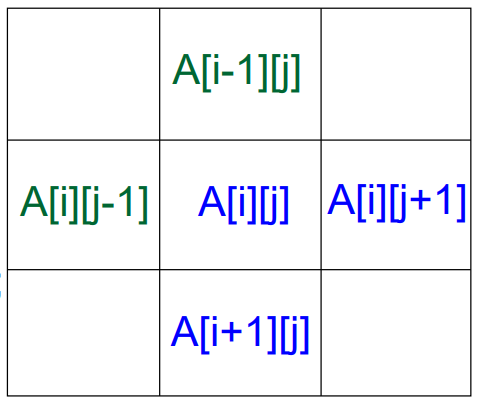
\includegraphics[width=0.6\textwidth]{images/grid.png}
    \caption{Grid points and their neighbours}
    \label{fig:grid}
\end{figure}

In each iteration, we sweep through all grid points, update the value at each point by averaging the values of its four (or more) immediate neighbours, and accumulate the absolute difference in the variable \texttt{diff}. We continue this process until \texttt{diff} falls below a given tolerance.

There are two classical iterative methods for this problem:

\begin{itemize}
    \item \textbf{Jacobi Method:} Uses neighbour values from the previous time step. All grid points are updated simultaneously using an auxiliary array to store the new values.
    
    \item \textbf{Gauss-Seidel Method:} Uses the most recently available values — i.e., when updating a grid point, the already-updated values from the current iteration (lower index values) are used whenever possible. This usually converges faster but is inherently more sequential.
\end{itemize}

To parallelize this computation, we need to decompose the grid into sub-regions that can be processed independently by different threads or processes. Each task will be responsible for a subset of grid points. However, care must be taken to handle boundary conditions and ensure proper synchronization or communication between tasks when accessing neighbouring values.

\begin{enumerate}
    \item One way is to consider each element in parallel. A parallel process or a parallel thread for each of the elements, i.e., a concurrent task for each element update. This would require a maximum concurrency of $n^2$ tasks (for $n \times n$ elements in the grid). Practically, this is not feasible as the number of tasks is very large, and the overhead of creating and managing the tasks is very high. This many parallel threads is not practically possible, as for larger values of $n$, the number of threads required will be $n^2$. Thus, many threads would have to be mapped to the same processors and would require a lot of context switching between threads and processes, which can affect the performance.

    \item Another way is to consider tasks for elements in the anti-diagonal. Note that values in a particular anti-diagonal depend on the values from the previous anti-diagonal but not among the elements within the same anti-diagonal. Now we consider a particular anti-diagonal—for some element in the anti-diagonal, using the Gauss-Seidel method, we require the values of the neighbours from the previous anti-diagonal at the latest time step and the value from the next anti-diagonal at the previous time step. This works out, since we are computing anti-diagonal by anti-diagonal, starting from the top-left corner and moving toward the bottom-right corner. Thus, the values of the neighbours are available from the previous anti-diagonal at the latest time step and the next anti-diagonal at the previous time step. Also, note that the values of the elements in the anti-diagonal are independent of each other and thus can be computed in parallel. This is as shown in the Figure~\ref{fig:anti-diag_examp}.
\begin{figure}[ht]
    \centering
    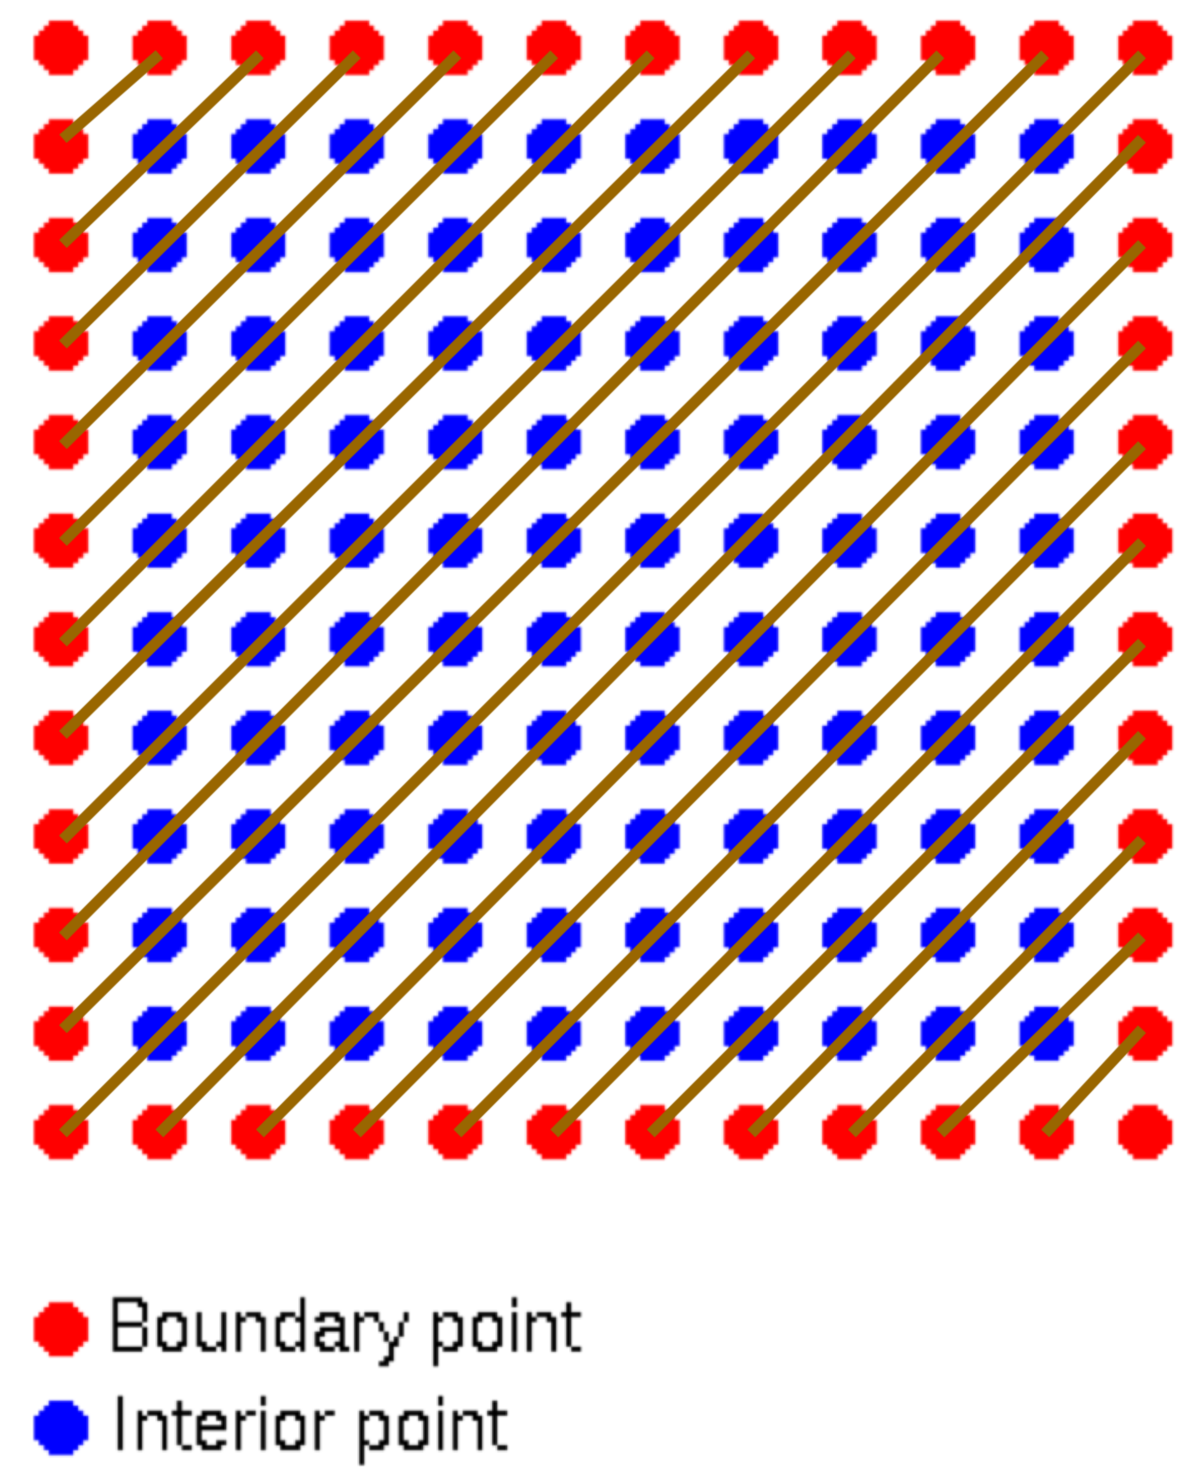
\includegraphics[width=0.5\linewidth]{images/Examp_anti2.png}
    \caption{Anti-diagonals}
    \label{fig:anti-diag_examp}
\end{figure}
    \vspace{5pt}
    Therefore, we can consider the tasks for the elements in the anti-diagonal and compute their values in parallel. This way, we can reduce the number of tasks to $2n - 1$ (for $n \times n$ elements in the grid). This is a better approach than the previous one, as the number of tasks is reduced and the tasks are independent of each other.

    \vspace{5pt}
    Note that for the diagonals at the ends, the number of elements will be smaller, and hence the parallelism will also be limited. This approach also incurs synchronization costs because the processes assigned to a particular diagonal cannot start executing until the earlier diagonals have finished executing. Thus, the parallelism is limited by the number of elements in the diagonal and the synchronization overhead.

    \item What we follow is block distribution of the data. Consider Figure~\ref{fig:block}, which shows the block distribution of the data.
    
    \begin{figure}[H]
        \centering
        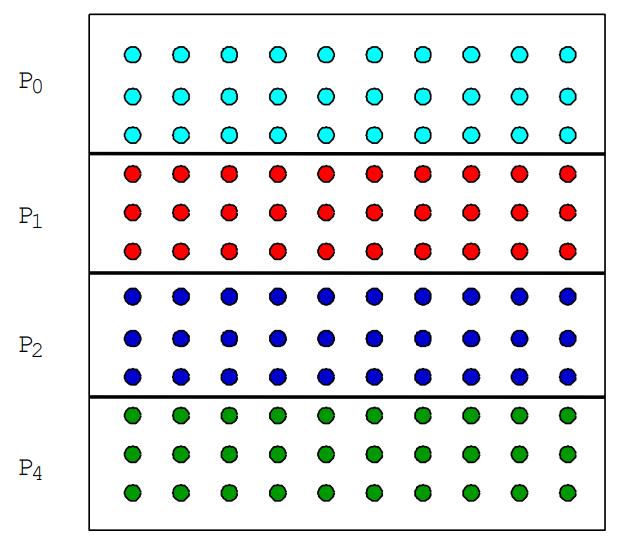
\includegraphics[width=0.6\textwidth]{images/block.png}
        \caption{Block Distribution}
        \label{fig:block}
    \end{figure}
    
    In this approach, we divide the 2D grid across the rows. The first set of rows is assigned to P0, the second set to P1, and so on. Each processor will be responsible for updating the values of the elements in the rows assigned to it.

    \vspace{5pt}
    For the orchestration step, we need to identify the synchronization and communication requirements. The goal is to ensure correctness while minimizing communication and synchronization calls. The implementation details depend on the underlying programming/model architecture—whether it is based on a shared memory model or a message-passing model.
\end{enumerate}


\subsubsection{Shared Address Space / Shared Memory Model}

Now we consider the Shared Address Space (SAS) version of the program, as shown in Listing~\ref{lst:shared}.

\begin{lstlisting}[style=cppstyle, caption={Shared Address Space Version}, captionpos=b, label={lst:shared}]
int n, nprocs; /* Matrix: (n+2) x (n+2) elements */
float **A, diff = 0;
LockDec(lock_diff);
BarrierDec(barrier1);

main()
begin
    read(n);           /* Read input parameter: matrix size */
    read(nprocs);      /* Read number of processors */
    
    A = malloc(a 2-D array of (n+2) x (n+2) floats);
    
    Create(nprocs - 1, Solve, A);  /* Spawn nprocs - 1 processes */
    
    initialize(A);     /* Initialize the matrix A */
    
    Solve(A);          /* Main process also solves */
    
    Wait_for_End(nprocs - 1);  /* Wait for other processes to finish */
end main
\end{lstlisting}

Note that we are using $(n+2)$ grid points to handle boundary conditions, but only \texttt{nprocs} processors. The array \texttt{A} is shared among all processes. The main process creates the other processes and then continues with solving. 

Let us now look at the pseudocode for the \texttt{Solve} function.

\begin{lstlisting}[style=cppstyle, caption={Solve Function}, captionpos=b, label={lst:solve}]
procedure Solve(A)  /* Solve the equation system */
float **A;
begin
    int i, j, pid, done = 0;
    float temp;

    mybegin = 1 + (n / nprocs) * pid;
    myend   = mybegin + (n / nprocs);

    while (!done) do  /* Outer loop over sweeps */
        diff = 0;  /* Initialize difference to 0 */

        Barrier(barrier1, nprocs);  /* Synchronize all processes */

        for (i = mybegin; i < myend; i++) do  /* Sweep over grid */
            for (j = 1; j <= n; j++) do
                temp = A[i][j];  /* Save old value */
                A[i][j] = 0.2 * (A[i][j] + A[i][j-1] + A[i-1][j] + A[i][j+1] + A[i+1][j]);  /* Compute average */
                diff += abs(A[i][j] - temp);
            end for
        end for

        if (diff / (n * n) < TOL) then
            done = 1;
    end while
end procedure
\end{lstlisting}



Now, this particular function is executed by all the processes. But depending on the process ID, different processes will handle different parts of the grid. This approach is called the \textbf{Single Program Multiple Data (SPMD)} model. The same program is executed by all processes, but each works on a different portion of the data.

The expressions 
\[
\texttt{mybegin} = 1 + \left(\frac{n}{\texttt{nprocs}}\right) \cdot \texttt{pid}, \quad \texttt{myend} = \texttt{mybegin} + \left(\frac{n}{\texttt{nprocs}}\right)
\]
determine the starting and ending rows of the grid that each process is responsible for. These are calculated using the process ID.

All the processes now enter the \texttt{while} loop. The matrix \texttt{A} and the variable \texttt{diff} are shared by all processes, making them global. At the beginning of each iteration, all processes synchronize using a \texttt{barrier}, as shown in the code.

Each process then executes the loop that updates a subset of the grid. Although every process runs the same code, they work on different rows depending on their \texttt{pid}. The elements in the grid are updated by computing an average, and the difference between the new and old values is added to \texttt{diff}.

Since \texttt{diff} is a shared variable, it gets updated by all the processes. At the end of the iteration, it is compared with a predefined tolerance to determine whether the loop should terminate.

This was just an overview of the program. To understand the benefits of parallel computing, it's important to appreciate synchronization primitives like the \texttt{barrier}.

A \texttt{barrier} is a synchronization point. When a process reaches a barrier, it waits there until all other processes have reached the same point. Only after that can any of the processes proceed. In the program above, this ensures that all processes finish their computation for one iteration before moving to the next. Without this, some processes might start the next iteration using stale values from neighboring processes that haven’t finished updating their part of the grid.

\begin{note}
    The matrix \texttt{A} is a global variable and is shared among all processes. During execution, each process updates its portion of the matrix. However, issues can arise at the boundaries between two adjacent processors.

    For example, if a process updates a boundary element before its neighboring process has finished updating its own value, inconsistent or stale values might be used. This can lead to incorrect results.

    One way to avoid this problem, especially in the Jacobi method, is to use a temporary array local to each process. This temporary array holds the updated values for the current iteration based on the global matrix values from the previous step. Once all processes have completed their local updates (ensured via a \texttt{barrier} call), the temporary arrays are copied back into the shared matrix \texttt{A}, and the next iteration begins.

    This ensures that all updates, especially at the boundaries, are synchronized. In our current discussion, we are ignoring this issue for simplicity and assuming that such synchronization is handled internally.
\end{note}
After solving the matrix \texttt{A}, the code in Listing~\ref{lst:shared} uses a \texttt{Wait\_for\_End} call. This makes the main process wait until all the other processes have finished. It can be implemented using an \textit{all-to-one} communication pattern, where each worker process sends a message to the main process to signal completion.

Note that the variable \texttt{diff} is a global (shared) variable. Since all processes read and write to it, it can lead to incorrect or garbage values due to race conditions. A race condition happens when multiple processes access and update a shared variable at the same time, leading to unpredictable results. This often arises because of context switching at the assembly level.

To solve this, we use \textbf{locks}. A lock is a mechanism that ensures only one process can access a shared resource at a time. When a process wants to update the shared variable, it first locks it, then accesses and modifies it, and finally unlocks it. This ensures exclusive access.

In computer science, a \textbf{lock} or \textbf{mutex} (short for mutual exclusion) is a synchronization primitive. It ensures that only one thread or process can acquire the lock at any given time. All other threads trying to acquire the lock are blocked until the lock is released. This ensures that shared resources are protected and accessed safely.

This concept is called \textbf{mutual exclusion} — processes exclude each other, allowing only one to enter the critical section (the part of the code accessing the shared variable). In our case, both \texttt{diff} and the matrix \texttt{A} are shared variables. So, care must also be taken when processes update boundary elements of the matrix. Those elements may be read and written by neighboring processes at the same time.

To avoid this, locks can also be used while updating matrix elements at the boundaries. However, another common and more efficient approach is to use a temporary matrix that is local to each process. Each process computes new values into its local matrix, based on the previous values in the global matrix. After all processes finish (synchronized using a \texttt{barrier}), they copy their local results into the global matrix. This approach is called \textbf{double buffering}.

Locks, while helpful, are expensive. If each grid point update needs to acquire a lock (especially for \texttt{diff}), it introduces a lot of waiting. Every process will have to wait for others to release the lock before updating \texttt{diff}. This adds overhead and reduces performance.

But here’s an observation: we only need \texttt{diff} at the end of each iteration — to check convergence. So, instead of updating the global \texttt{diff} every time, each process can maintain a \texttt{mydiff} variable locally. At the end of the iteration, all local \texttt{mydiff} values are added together to get the global \texttt{diff}. This is called a \textbf{reduction operation}. It significantly reduces locking overhead.

Previously, locks were required for each of the $\mathcal{O}(n^2)$ grid updates. Now, with local diffs and a single reduction step, we reduce the locking overhead to $\mathcal{O}(p)$, where $p$ is the number of processes — a huge improvement!

The updated \texttt{Solve} function with this idea is shown in Listing~\ref{lst:solve2}.

\begin{lstlisting}[style=cppstyle, caption={Updated Solve Function}, captionpos=b, label={lst:solve2}]
procedure Solve(A)  /* Solve the equation system */
float **A;
begin
    int i, j, pid, done = 0;
    float mydiff, temp;

    mybegin = 1 + (n / nprocs) * pid;
    myend   = mybegin + (n / nprocs);

    while (!done) do  /* Outer loop over sweeps */
        mydiff = diff = 0;  /* Initialize differences */

        Barrier(barrier1, nprocs);  /* Synchronize before sweep */

        for (i = mybegin; i < myend; i++) do  /* Grid sweep */
            for (j = 1; j <= n; j++) do
                temp = A[i][j];  /* Save old value */
                A[i][j] = 0.2 * (A[i][j] + A[i][j-1] + A[i-1][j] + A[i][j+1] + A[i+1][j]);
                mydiff += abs(A[i][j] - temp);
            end for
        end for

        lock(diff-lock);
            diff += mydiff;  /* Accumulate local diff to global diff */
        unlock(diff-lock);

        Barrier(barrier1, nprocs);  /* Synchronize before checking */

        if (diff / (n * n) < TOL) then
            done = 1;  /* Check convergence */
        
        Barrier(barrier1, nprocs);  /* Final barrier before next sweep */
    end while
end procedure
\end{lstlisting}
Note that in the updated pseudocode, a new local variable \texttt{mydiff} is introduced for each process. This variable is updated independently by each process during the iteration. At the end of the iteration, all local \texttt{mydiff} values are added together to get the global \texttt{diff} value, using the locking mechanism as shown in Listing~\ref{lst:solve2}.

The statements \texttt{lock(diff-lock)} and \texttt{unlock(diff-lock)} are used to acquire and release the lock on the shared \texttt{diff} variable. This reduces the contention for the lock, since it is needed only once per process per iteration, not for every grid point update.

A \texttt{barrier} call is placed after the accumulation step. This ensures that all processes have completed their computations and updated the global \texttt{diff} before any process checks the termination condition. Without this synchronization, some processes might check the condition before \texttt{diff} is fully updated, leading to incorrect results.

Another \texttt{barrier} is placed right after the termination condition check. This is important because if the condition is not met, one process might enter the next iteration and set \texttt{diff = 0} too early. Meanwhile, another process still evaluating the condition might see this incorrect zero value, which would be wrong. The second barrier ensures that all processes finish checking the correct value of \texttt{diff} before any of them proceed to the next iteration.

The assignment \texttt{done = 1} is done redundantly by all processes once convergence is reached. This is acceptable because the statement is identical to what appears in a sequential program.

This brings us to an important point. One of the advantages of shared memory programming is that the code structure remains close to the sequential version. Parallelism is introduced simply by adding constructs like \texttt{locks} and \texttt{barriers}. This makes shared memory programs easier to write and debug compared to message passing programs, where the entire structure is different and processes need to explicitly communicate using send and receive operations.


\subsubsection{Message Passing Version}

In the message passing model, we cannot assume that matrix \texttt{A} is a global shared array accessible to all processes. There is no concept of shared variables here. Each process must maintain its own local part of the matrix.

If a process needs values that were updated by another process, it must explicitly receive them through message passing. So, data has to be sent between processes.

We use \textit{domain decomposition} to divide the 2D domain among different processes. Each process follows the \textit{owner computes} rule, meaning the process responsible for a subdomain also computes values in that region.

Since there is no global data structure, each process maintains local data structures. This increases the need for communication. To handle this, we introduce something called \textbf{ghost rows}.

Ghost rows are explained in Figure~\ref{fig:ghost}.

\begin{figure}[H]
    \centering
    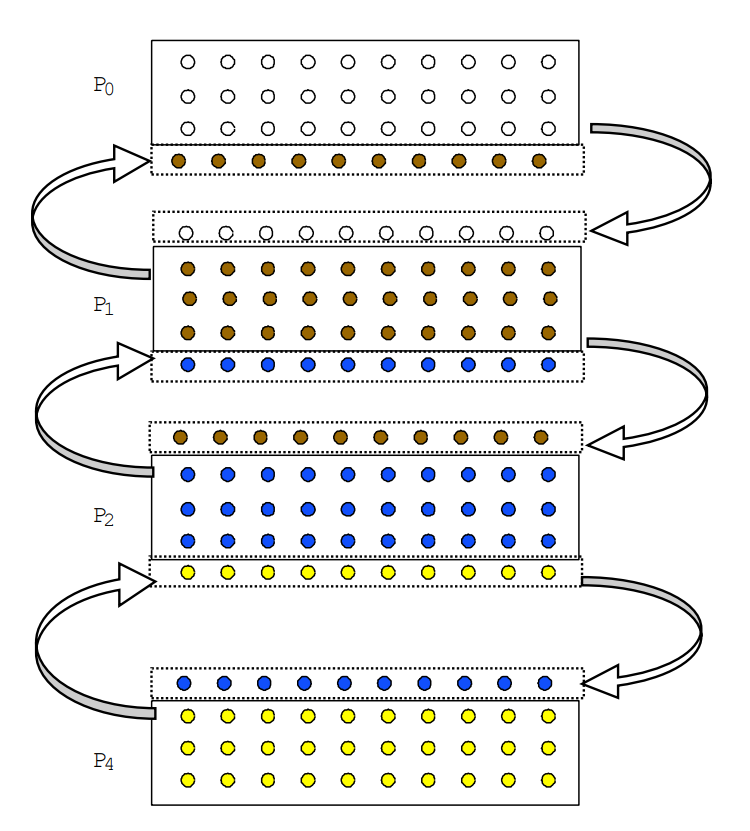
\includegraphics[width=0.6\textwidth]{images/ghost.png}
    \caption{Ghost Rows}
    \label{fig:ghost}
\end{figure}

In this figure~\ref{fig:ghost}, the 2D grid is divided among 4 processes, just like in the shared memory model. Each process is responsible for updating values in its assigned rows.

But unlike the shared memory model, each process now has its own local array to store these rows. In addition to this, each process has extra rows called \textbf{ghost rows}, as shown in the figure.

These ghost rows are used to store boundary values received from neighboring processes. For example:
\begin{itemize}
    \item Process 0 has a ghost row at the bottom to store the top boundary row from Process 1.
    \item Process 1 has a ghost row at the top for Process 0 and at the bottom for Process 2.
    \item And so on for the other processes.
\end{itemize}

Ghost rows are not updated by the process that holds them. Instead, they are updated by the neighboring processes that own the actual data. The purpose of ghost rows is to help compute local values at the boundaries using up-to-date data from neighbors.

Ghost rows are also called \textit{halo rows}, \textit{halo regions}, or \textit{ghost zone regions}.

Once each process receives the required ghost row data from its neighbors, it can simply perform local (sequential) computation using its local array.

Now consider the message passing version of the program shown in Listing~\ref{lst:mpi}.

\begin{lstlisting}[style=cppstyle,caption={Message Passing Version - Main Function},captionpos=b,label={lst:mpi}]
int n, nprocs; /* matrix: (n+2) x (n+2) elements */
float **myA;

main()
begin
    read(n);           /* read input parameter: matrix size */
    read(nprocs);      /* read number of processes */
    A = malloc(a 2-D array of (n+2) x (n+2) doubles);
    Create(nprocs-1, Solve, A);
    initialize(A);     /* initialize the matrix A somehow */
    Solve(A);
    Wait_for_End(nprocs-1);
end main
\end{lstlisting}


Now consider the \texttt{Solve} function for the message passing version, shown in Listing~\ref{lst:solve3}, which includes array allocation and ghost row communication.

\begin{lstlisting}[style=cppstyle,caption={MPI - Solve Function},captionpos=b,label={lst:solve3}]
procedure Solve(A) /* solve the equation system */
    float **A; /* A is a (n+2)-by-(n+2) array
begin
    int i, j, pid, done = 0;
    float mydiff, temp;
    myend = (n / nprocs);
    myA = malloc(array of (n / nprocs) x (n) floats);
    intialize(myA); /* Intialization myA locally*/
    
    while (!done) do /* outermost loop over sweeps */
        mydiff = 0; /* initialize local difference to 0 */

        if (pid != 0) then
            SEND(&myA[1,0], n * sizeof(float), (pid - 1), row);
        if (pid != nprocs - 1) then
            SEND(&myA[myend,0], n * sizeof(float), (pid + 1), row);
        if (pid != 0) then
            RECEIVE(&myA[0,0], n * sizeof(float), (pid - 1), row);
        if (pid != nprocs - 1) then
            RECEIVE(&myA[myend + 1,0], n * sizeof(float), (pid + 1), row);

        for (i = 1 to myend) do
            for (j = 1 to n) do
                temp = A[i,j]; /* save old value */
                A[i,j] = 0.2 * (A[i,j] + A[i,j-1] + A[i-1,j] + A[i,j+1] + A[i+1,j]); /* compute average */
                mydiff += abs(A[i,j] - temp);
            end for
        end for

        if (pid != 0) then
            SEND(mydiff, sizeof(float), 0, DIFF);
            RECEIVE(done, sizeof(int), 0, DONE);
        else
            for k = 1 to nprocs - 1 do
                RECEIVE(tempdiff, sizeof(float), k, DIFF);
                mydiff += tempdiff;
            end for
            if (mydiff / (n * n) < TOL) then done = 1;
            for k = 1 to nprocs - 1 do
                SEND(done, sizeof(int), k, DONE);
            end for
    end while
end procedure
\end{lstlisting}

In Listing~\ref{lst:solve3}, \texttt{myA} is the local array for each process. It stores the values of the grid elements corresponding to the domain allocated to the process—some subset of rows and all columns.

There are multiple ways to initialize these arrays: one option is to have each process read from a file; another is to let one process initialize the entire matrix and then distribute chunks to the others. For simplicity, we assume the processes are somehow able to initialize their local matrices.

Inside the \texttt{while} loop, each process maintains a local \texttt{mydiff} variable (note: no shared memory, so each process computes this separately).

At the start of each iteration, every process exchanges boundary rows with its neighboring processes:
\begin{itemize}
    \item If \texttt{pid} $\neq$ 0, the process sends its top row to \texttt{pid - 1}.
    \item If \texttt{pid} $\neq$ \texttt{nprocs - 1}, it sends its bottom row to \texttt{pid + 1}.
    \item Then, it receives the boundary rows from its neighbors and stores them in its \textbf{ghost rows}.
\end{itemize}

The ghost rows allow a process to compute its inner grid points using up-to-date boundary values received from neighbors. These ghost rows are only used for reading during the computation and are updated only via explicit communication (not by the owning process).

Once the ghost rows are updated, each process updates its portion of the grid just like in the sequential version. It also calculates its local difference \texttt{mydiff} during the update.

After computation:
\begin{itemize}
    \item Non-zero processes send their \texttt{mydiff} to process 0.
    \item Process 0 receives all \texttt{mydiff} values, aggregates them into a global \texttt{diff}, and checks the convergence condition.
    \item If convergence is met, it sends a \texttt{done} signal to all other processes.
    \item All processes exit the loop when \texttt{done = 1}.
\end{itemize}

This is how the message passing version of the program works using MPI-style pseudocode.


\subsection{Notes on Message Passing Version}

\begin{itemize}
    \item In the shared memory model, although there's no explicit communication, when one process writes to a variable and another reads it, this can still be seen as a form of communication. However, it is \textbf{receiver-initiated}, meaning the communication completes when the receiving process accesses the variable.

    \item In contrast, in the message passing model, communication is \textbf{sender-initiated}. A process must explicitly send data to another process using message-passing primitives like \texttt{SEND} and \texttt{RECEIVE}.

    \item Synchronization in the message passing model is \textbf{implicit}. Unlike in the shared memory model where synchronization is often done using explicit barriers, here it happens through communication operations. For instance, a \texttt{SEND} and \texttt{RECEIVE} pair naturally synchronizes two processes.

    \item This brings up a critical question: \textbf{can deadlocks occur in MPI communication?} Yes, they can. A deadlock may happen if all processes are stuck waiting for others to send data while none are sending anything.

    For example:
    \begin{itemize}
        \item All processes issue a \texttt{RECEIVE} before any \texttt{SEND}. Since no data is being sent, all processes block and wait indefinitely.
        \item Alternatively, all processes issue a blocking \texttt{SEND} that only completes when the data is received. But since no process is yet ready to receive, all \texttt{SEND}s block, leading again to a deadlock.
    \end{itemize}

    \item To avoid such situations, we can use \textbf{non-blocking communication} or design the program so that at least one process starts with a \texttt{SEND} and another with a \texttt{RECEIVE}.

    \item Such communication is called \textbf{synchronous communication}, where the \texttt{SEND} completes only after the matching \texttt{RECEIVE} starts. This ensures synchronization between processes.

    \item Communication is performed in entire rows at the beginning of each iteration — not point-by-point. This means an entire row is sent in one go instead of sending one grid point at a time, which is more efficient.

    \item Observe the communication pattern where each process sends its \texttt{mydiff} value to process 0, which aggregates all values to compute the global difference. This is an \textbf{All-to-One communication pattern}, known as a \textbf{reduction}.

    \item Reduction is a common pattern in parallel programming. Many parallel libraries provide built-in support for such operations. In this case, we add the local \texttt{mydiff} values using a reduction operation.

    \item After computing the global difference, the master process (process 0) broadcasts the \texttt{done} signal to all other processes. This is a \textbf{One-to-All communication}, also known as a \textbf{broadcast}.

    \item The original code using \texttt{SEND} and \texttt{RECEIVE} can be simplified using \texttt{REDUCE} and \texttt{BROADCAST} operations, as shown below:

\begin{lstlisting}[style=cppstyle]
/* Communicate local diff values and determine if done,
   using reduction and broadcast */
REDUCE(0, mydiff, sizeof(float), ADD);
if (pid == 0) then
    if (mydiff / (n * n) < TOL) then
        done = 1;
    endif
    BROADCAST(0, done, sizeof(int), DONE);
\end{lstlisting}

    \item The \texttt{REDUCE} operation collects the \texttt{mydiff} values from all processes at process 0 using an \texttt{ADD} operator to compute the global difference. Other operators like \texttt{MAX}, \texttt{MIN}, etc., can also be used depending on the need.

    \item After checking the termination condition, the master process uses \texttt{BROADCAST} to send the \texttt{done} signal to all other processes. This makes the communication more concise and efficient.
\end{itemize}


\subsection{Send and Receive Alternatives}

Recall that in the message-passing version, we used the \texttt{SEND} and \texttt{RECEIVE} operations to communicate data between processes. However, it may happen that the \texttt{SEND} operation causes the sending process to wait until the corresponding receiving process initiates its \texttt{RECEIVE} operation, and vice versa. This mutual waiting results in synchronous communication, where both sender and receiver are blocked until the message transfer is complete.

To avoid this blocking behavior, asynchronous communication can be used. Many MPI libraries support asynchronous \texttt{SEND} and \texttt{RECEIVE} operations, where a process does not need to wait for the corresponding operation on the other process to begin. In an asynchronous \texttt{SEND}, the sender proceeds without waiting for the receiver to initiate the \texttt{RECEIVE}. Similarly, in an asynchronous \texttt{RECEIVE}, the receiver does not block waiting for the sender to begin transmission.

Asynchronous operations can be further categorized into \textbf{blocking asynchronous} and \textbf{non-blocking asynchronous} variants. These will be discussed in detail in the MPI section.

\subsection{Summary}

\begin{itemize}
    \item \textbf{Shared Address Space (SAS)}: Shared and private data are explicitly separated. Communication occurs implicitly through shared memory access patterns. Synchronization is explicit, typically performed via atomic operations such as locks and barriers.
    
    \item \textbf{Message Passing}: There is no concept of shared memory; all data structures reside in local address spaces. Communication is explicit via \texttt{SEND} and \texttt{RECEIVE} operations. In the example discussed, synchronization is implicit—no explicit barrier is used—but explicit synchronization constructs also exist in message-passing models.
    
    \item While decomposition and assignment strategies were similar in both SAS and message-passing models, the key differences lie in orchestration and mapping. Table~\ref{tab:finsummary} summarizes the comparison:
\end{itemize}

\begin{table}[H]
    \centering
    \begin{tabular}{|p{0.5\textwidth}|c|c|}
        \hline
        & \textbf{Shared Address Space} & \textbf{Message Passing} \\
        \hline
        Explicit in global structure? & Yes & No \\
        Communication                 & Implicit & Explicit \\
        Synchronization               & Explicit & Implicit \\
        Explicit replication of border rows? & No & Yes \\
        \hline
    \end{tabular}
    \caption{Comparison between Shared Address Space and Message Passing Models}
    \label{tab:finsummary}
\end{table}
For more details on parallelization principles refer to sections 3.1 and 3.5 in~\cite{kumar1994introduction} and sections 2.2 and 2.3 in~\cite{culler1998parallel} for example.

\chapter{Shared Memory Parallelism - OpenMP}

Recall the term \textbf{processes} used in the context of shared memory address space models. In this setting, the term typically refers to \textbf{threads}. Threads are lightweight processes that share the same address space. Since multiple threads can access shared variables concurrently, synchronization mechanisms like barriers and locks are required to ensure data consistency and avoid race conditions.

The programmer must explicitly specify which variables are shared across threads and which are private to each thread. Because threads operate within the same address space, they can access common data structures and variables directly.

The most widely used programming interface for shared memory parallelism is OpenMP (Open Multi-Processing), a portable and scalable programming model. OpenMP provides a set of compiler directives, library routines, and environment variables to express parallelism at a high level in Fortran, C, and C++ programs.

So, what are compiler directives? These are special annotations or statements within the code that instruct the compiler to perform certain actions. For example, compilers support various optimization levels like \texttt{-O1}, \texttt{-O2}, etc. Through compiler directives, you can direct the compiler to optimize specific parts of the code selectively. In OpenMP, such directives are used to express shared-memory parallelism and are often referred to as \textbf{pragmas}.

One of the key advantages of OpenMP is that it makes parallel programming relatively simple. You can start with a serial program, then gradually insert OpenMP directives to indicate parallel regions, and finally compile and run the program with appropriate OpenMP flags to enable parallel execution.

The first version of OpenMP was released in 1997. As of now, the widely used version is OpenMP 6.0, released in 2024.


\section{Fork-Join Model}

OpenMP follows the \textbf{fork-join} execution model. The program begins with a single thread, known as the \textit{master thread}. When the program encounters a parallel construct, the master thread \textit{forks} a team of worker threads to execute the parallel region. Once the parallel region is completed, the worker threads \textit{join} back into the master thread, and execution resumes sequentially.

This behavior is illustrated in Figure~\ref{fig:forkjoin}.

\begin{figure}[H]
    \centering
    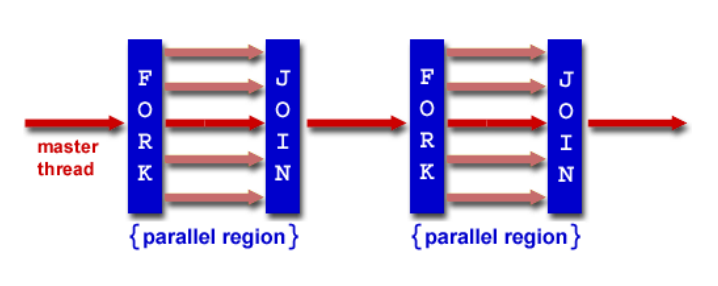
\includegraphics[width=0.6\textwidth]{images/forkjoin.png}
    \caption{Fork-Join Model}
    \label{fig:forkjoin}
\end{figure}

As seen in the figure, a single thread starts executing the program. Upon encountering a parallel region, a team of threads is spawned to execute that block in parallel. After completion, the threads synchronize and terminate, returning control to the master thread.

One of the major advantages of OpenMP is its support for \textbf{selective parallelism}—only specific regions of the code are parallelized based on need. This aligns well with \textbf{Amdahl's Law}, which highlights that only parts of a program are parallelizable while others must remain serial. OpenMP does not attempt to parallelize the entire program but instead allows the programmer to specify which regions benefit most from parallel execution.

OpenMP provides several key constructs to support parallel programming:
\begin{itemize}
    \item \textbf{Work-sharing constructs:} Specify how the work in a parallel region should be divided among the threads.
    \item \textbf{Synchronization constructs:} Ensure proper coordination and data consistency between threads.
    \item \textbf{Data environment constructs:} Define which variables are shared across threads and which are private to each thread.
    \item \textbf{Library routines and environment variables:} Provide utility functions and allow customization of the execution environment (e.g., setting the number of threads using environment variables before program execution).
\end{itemize}

A \textit{construct} in OpenMP refers to a compiler directive paired with the block of code (region) to which it applies.

OpenMP primarily supports \textbf{loop-level parallelism}, especially for \texttt{for}/\texttt{do} loops. If there are no loop-carried dependencies, iterations can be safely divided among threads. Each thread then executes a subset of the loop iterations. This offers \textbf{fine-grained parallelism}, giving the programmer detailed control over which specific regions of code are parallelized.

Additionally, OpenMP allows \textbf{dynamic parallelism}—the number of threads used in a parallel region can be varied based on computational load. Regions that benefit from greater parallelism can use more threads, while lighter regions may use fewer. This flexibility is useful for optimizing performance dynamically at runtime.

Alongside fine-grained parallelism, OpenMP also supports \textbf{coarse-grained parallelism}, where entirely different sections of the program are executed in parallel.

Modern versions of OpenMP include advanced features such as:
\begin{itemize}
    \item \textbf{Offloading to accelerators (e.g., GPUs):} Through target directives, specific regions of code can be executed on devices such as GPUs.
    \item \textbf{SIMD vectorization:} Enables automatic vectorized execution of operations across multiple data elements.
    \item \textbf{Task-core affinity:} Allows tasks to be pinned to specific cores, which can help reduce data movement and improve cache utilization.
\end{itemize}

These features make OpenMP not just a tool for simple parallelism, but a comprehensive framework suitable for modern multicore and heterogeneous architectures.


\section{Parallel Construct}

\texttt{\#pragma omp parallel} is the primary parallel construct in OpenMP.  
It is used to create a \textbf{team of threads}, where each thread executes the specified code block in parallel. The syntax is:

\begin{lstlisting}[style=cppstyle]
#pragma omp parallel
{
    /* parallel region */
}
\end{lstlisting}

This block of code is referred to as the \textbf{parallel region}. When the compiler encounters the \texttt{\#pragma omp parallel} directive, it forks a team of threads. Each thread in the team executes the code inside the braces.  
Before this directive is reached, the program executes sequentially on the \textbf{master thread}.

Thus, a \textbf{parallel construct} consists of the `parallel` directive and the corresponding code block that is executed concurrently by multiple threads.

\vspace{0.5em}
\noindent
\textbf{How many threads are created?}
This depends on how OpenMP is configured. There are several ways to control the number of threads:

\begin{itemize}
    \item Set the environment variable at runtime: \texttt{export OMP\_NUM\_THREADS=number}
    \item Use the function call: \texttt{omp\_set\_num\_threads(n);}
    \item Use the clause \texttt{num\_threads(n)} directly in the pragma directive.
\end{itemize}

\vspace{0.5em}
\noindent
OpenMP also provides various \textbf{clauses} to modify the behavior of the parallel region:

\begin{itemize}
    \item \texttt{if (condition)}: Executes the parallel region in parallel only if the condition evaluates to true; otherwise, it is executed serially by the master thread.
    \item \texttt{num\_threads(n)}: Specifies the exact number of threads to be used in the parallel region.
    \item \texttt{default(shared | none)}: Sets the default data-sharing attributes for variables—either shared or requiring explicit declaration.
    \item \texttt{private(list)}: Declares a list of variables that are private to each thread. Each thread gets its own uninitialized copy.
    \item \texttt{firstprivate(list)}: Like `private', but initializes each thread’s copy with the value of the variable outside the parallel region.
    \item \texttt{shared(list)}: Declares a list of variables to be shared across all threads.
    \item \texttt{copyin(list)}: For variables declared `threadprivate`, initializes the value of each thread’s copy with that of the master thread.
    \item \texttt{reduction(operator: list)}: Each thread gets a private copy of the listed variables, which are combined at the end of the parallel region using the specified operator (like `+', `*', `max', etc.).
    \item \texttt{proc\_bind(master | close | spread)}: Controls thread-to-core binding. `master' binds threads to the same core as the master thread; `close' places them on nearby cores; `spread' distributes them across cores.
\end{itemize}

\vspace{0.5em}
\noindent
Consider the following example, which prints the number of threads created inside a parallel region:

\begin{lstlisting}[style=cppstyle]
#include <omp.h>
#include <stdio.h>

int main()
{
    int nthreads;
    #pragma omp parallel
    {
        nthreads = omp_get_num_threads();
        printf("Number of threads = %d\n", nthreads);
    }
    return 0;
}
\end{lstlisting}

If, say, 4 threads were used, you’ll see the line "Number of threads = 4" printed 4 times—once by each thread.

\vspace{0.5em}
\noindent
Now consider a basic Hello World example in OpenMP:

\begin{lstlisting}[style=cppstyle]
#include <omp.h>
#include <stdio.h>

int main()
{
    int nthreads, tid;
    #pragma omp parallel private(nthreads, tid)
    {
        tid = omp_get_thread_num();
        printf(``Hello World from thread %d\n", tid);
    }
    return 0;
}
\end{lstlisting}

Here, each thread prints its own message. The `private' clause ensures that `tid' and `nthreads' are thread-local, preventing race conditions. Try running this code on your machine to see multiple "Hello World" messages printed in parallel.

\vspace{0.5em}
\noindent
OpenMP makes it straightforward to parallelize sequential programs incrementally. You can write the core logic sequentially and then wrap performance-critical sections with appropriate OpenMP constructs.

\section{Work Sharing Construct}
The work sharing construct in OpenMP is used to distribute work among multiple threads. Once multiple threads have been spawned using the \texttt{parallel} construct, the work sharing construct specifies how the workload should be divided among these threads.

There are three main types of work sharing constructs in OpenMP:
\begin{itemize}
    \item \textbf{loops} – used to distribute iterations of a loop among threads,
    \item \textbf{sections} – used to assign distinct code blocks to different threads,
    \item \textbf{single} – ensures that a particular block of code is executed by only one thread.
\end{itemize}


\subsection{for-loop}

The \texttt{for} construct is used to parallelize \texttt{for}-loops or \texttt{do}-loops in OpenMP using the syntax:
\begin{lstlisting}[style=cppstyle]
#pragma omp for [clause[, clause]...]
\end{lstlisting}

It is typically used inside a \texttt{parallel} region to distribute loop iterations among the threads. The following clauses can be used with the \texttt{for} construct:

\begin{itemize}
    \item \textbf{private(list)}: Specifies variables that are private to each thread.
    \item \textbf{firstprivate(list)}: Like \texttt{private}, but initializes each private copy with the value of the original variable.
    \item \textbf{lastprivate(list)}: The variable is made private, but its value from the last iteration is copied back after the loop.
    \item \textbf{linear(list)}: Specifies linear induction variables with a fixed step size.
    \item \textbf{reduction(operator:list)}: Performs a reduction on the specified variables using the given operator across threads.
    \item \textbf{schedule([modifier:]kind[,chunk])}: Controls how iterations are divided among threads.
    \item \textbf{collapse(n)}: Useful for nested loops—collapses \texttt{n} nested loops into a single loop with a larger iteration space for parallelization.
    \item \textbf{ordered(n)}: Enforces ordered execution for sections of code marked with \texttt{ordered}.
    \item \textbf{nowait}: Prevents implicit barrier synchronization at the end of the loop. Threads need not wait for others.
\end{itemize}

The \texttt{for} construct is one of the most commonly used and important constructs in OpenMP. It assumes that loop iterations are independent of one another, i.e., there are no dependencies between iterations. If such dependencies exist—e.g., an iteration relies on the result of a previous iteration—then the \texttt{for} construct should not be used.

\paragraph{Schedule Clause:}  
The \texttt{schedule} clause determines how loop iterations are assigned to threads. OpenMP supports several scheduling policies:

\begin{enumerate}
    \item \textbf{schedule(static, chunk)}: Divides the iteration space into equal-sized chunks (of size \texttt{chunk}) and assigns them to threads in round-robin fashion.
    
    For example, consider a loop with 20 iterations and a chunk size of 2. Ten chunks are created, and with four threads, chunks are assigned as:
    \[
    \text{Thread 0: } \text{chunk 0, 4, 8}; \quad \text{Thread 1: } \text{chunk 1, 5, 9}; \text{...}
    \]

    \item \textbf{schedule(dynamic, chunk)}: Also splits the loop into chunks, but assigns them to threads dynamically at runtime. Threads that finish early can grab the next available chunk.
    
    \item \textbf{schedule(runtime)}: Defers scheduling strategy selection to runtime based on environment variables or OpenMP runtime configuration.
\end{enumerate}

\paragraph{Example:} Consider the following program that performs element-wise addition of two arrays:

\begin{lstlisting}[style=cppstyle, caption={Addition of Two Arrays Using \texttt{for} Construct}, label={lst:for-example}]
#include <omp.h>
#define CHUNKSIZE 100
#define N 1000

int main(){
    int i, chunk;
    float a[N], b[N], c[N];

    // Initialization
    for (i = 0; i < N; i++)
        a[i] = b[i] = i * 1.0;

    chunk = CHUNKSIZE;

    #pragma omp parallel shared(a, b, c, chunk) private(i)
    {
        #pragma omp for schedule(dynamic, chunk) nowait
        for (i = 0; i < N; i++) {
            c[i] = a[i] + b[i];
        }
    }

    return 0;
}
\end{lstlisting}

In this example, we are adding arrays \texttt{a} and \texttt{b} to produce \texttt{c}. Since each element-wise addition is independent, this is a good candidate for parallelization.

We use \texttt{\#pragma omp parallel} to create threads. The variables \texttt{a}, \texttt{b}, \texttt{c}, and \texttt{chunk} are marked as \texttt{shared} because they need to be accessed by all threads, while \texttt{i} is marked as \texttt{private} since each thread should have its own loop counter to avoid conflicts.

The inner \texttt{for} loop is parallelized using the \texttt{for} construct with \texttt{schedule(dynamic, chunk)} to allow dynamic load balancing. The \texttt{nowait} clause prevents threads from waiting for others once their iterations are complete.

Note that the two pragmas can be combined into a single directive as follows:

\begin{lstlisting}[style=cppstyle]
#pragma omp parallel for shared(a, b, c, chunk) private(i) schedule(dynamic, chunk) nowait
\end{lstlisting}


\subsection{Coarse-Level Parallelism — Sections and Tasks}

In addition to fine-level parallelism (as seen in the \texttt{for} loop example), OpenMP supports \textbf{coarse-level parallelism}. 

While fine-level parallelism typically deals with distributing iterations of a loop among multiple threads, coarse-level parallelism involves executing \textbf{independent blocks of code}—like separate functions or computational phases—in parallel.

\paragraph{Sections Construct:}
If we want to execute two or more independent code blocks (e.g., different functions) concurrently, OpenMP provides the \texttt{sections} construct. This allows different threads to execute different code blocks in parallel, rather than all threads executing the same block of code as in \texttt{for} loops.

Consider the example shown in listing \ref{lst:sections}:

\begin{lstlisting}[style=cppstyle, caption={Sections Construct}, captionpos=b, label={lst:sections}]
#pragma omp parallel sections [clauses]
{
    #pragma omp section
    {
        // structure block i (e.g., function1());
    }

    #pragma omp section
    {
        // structure block j (e.g., function2());
    }
    ...
}
\end{lstlisting}

In this example, each \texttt{\#pragma omp section} defines a code block (or task) that can be executed by a separate thread. The enclosing \texttt{parallel sections} directive spawns a team of threads, and each section is assigned to one thread for execution. This is useful when you have multiple, independent tasks that can be run concurrently.

\paragraph{Tasks Construct:}

OpenMP also supports dynamic task creation using the \texttt{task} construct. This is useful in scenarios such as recursive algorithms, adaptive simulations, or when the number and structure of tasks are not known in advance.

Inside a parallel region, individual threads can create tasks using the \texttt{task} directive. These tasks are then dynamically assigned to available threads by the OpenMP runtime system. This enables load balancing and fine control over task execution.

Here’s a simplified example of the \texttt{task} construct, shown in listing \ref{lst:tasks}:

\begin{lstlisting}[style=cppstyle, caption={Tasks Construct}, captionpos=b, label={lst:tasks}]
#pragma omp parallel
{
    #pragma omp single
    {
        #pragma omp task
        {
            // Task 1 code
        }

        #pragma omp task depend(in: x)
        {
            // Task 2 depends on variable x from Task 1
        }
    }
}
\end{lstlisting}

In the above code:

- \texttt{\#pragma omp single} ensures only one thread in the team creates tasks (preventing all threads from redundantly spawning the same tasks).
- \texttt{\#pragma omp task} defines a task to be executed by any thread.
- The \texttt{depend} clause allows specifying task dependencies.

\paragraph{Task Dependencies and Task Graphs:}

OpenMP's \texttt{depend} clause enables you to define data dependencies between tasks. For instance, if Task 2 depends on a variable modified by Task 1, you can ensure that Task 2 will only execute once Task 1 has completed. This forms a \textbf{task dependency graph}, where:
\begin{itemize}
\item \textbf{Nodes} represent tasks.
\item \textbf{Edges} represent dependencies.
\end{itemize}
The OpenMP runtime builds and schedules this graph automatically, respecting the constraints provided. This powerful feature enables writing highly dynamic and dependency-aware parallel programs.

Thus, tasks enable \textbf{dynamic coarse-level parallelism} where the number and structure of tasks can evolve during runtime, while also maintaining control over execution order through explicit dependencies.


\section{Synchronization Directives}

Once the work is distributed among threads, there is always a possibility that multiple threads may access and update common variables simultaneously. This can lead to race conditions and inconsistent results. Therefore, we need to synchronize threads and protect shared data using appropriate locking or ordering mechanisms.

OpenMP provides several synchronization directives for this purpose. Note that all these constructs must be enclosed within a parallel region (created by a parallel construct):

\begin{itemize}
    \item \texttt{\#pragma omp master}: The block of code following this directive is executed only by the master thread. This is useful, for example, when only one thread (typically the master) should perform tasks like printing to the console to avoid cluttered output.

    \item \texttt{\#pragma omp critical}: Ensures that the enclosed block is executed by only one thread at a time. This is useful for updating shared variables, where concurrent access by multiple threads could lead to inconsistent or garbage values.

    \item \texttt{\#pragma omp barrier}: Forces all threads in the team to wait at this point until every thread has reached it. Useful for synchronization at intermediate stages of the parallel region.

    \item \texttt{\#pragma omp atomic}: Ensures that the specific memory operation (such as a simple update to a variable) following this directive is executed atomically—only one thread performs the update at a time, but with lower overhead than a full critical section.

    \item \texttt{\#pragma omp ordered}: Specifies that the block of code should be executed in the order of thread IDs. This is helpful when we need ordered output—for example, when printing parts of an array sequentially from multiple threads.

    \item \texttt{\#pragma omp flush}: Ensures memory consistency between threads by forcing a thread’s private view of memory to be synchronized with shared memory. This is particularly useful when a thread updates a shared variable, and other threads must see the updated value immediately.

    Consider the following example using the \texttt{flush} directive, shown in listing \ref{lst:flush}.

\begin{lstlisting}[style=cppstyle, caption={Flush Directive}, captionpos=b, label={lst:flush}]
int sync[NUMBER_OF_THREADS];
float work[NUMBER_OF_THREADS];

#pragma omp parallel private(iam, neighbor) shared(work, sync)
{
    iam = omp_get_thread_num();
    sync[iam] = 0;
    #pragma omp barrier

    // Perform computation and write result to shared array
    work[iam] = compute(iam);

    // Announce completion of work
    #pragma omp flush(work)      // Ensure work is visible to other threads
    sync[iam] = 1;
    #pragma omp flush(sync)      // Ensure sync is updated in shared memory

    // Wait for neighbor to complete its work
    neighbor = (iam > 0 ? iam : omp_get_num_threads()) - 1;
    while (sync[neighbor] == 0) {
        #pragma omp flush(sync)
    }

    // Read neighbor's result
    ... = work[neighbor];
}
\end{lstlisting}

In this example, each thread computes its result and writes it to the shared \texttt{work} array. Neighboring threads need access to this data, so we use the \texttt{flush} directive to ensure memory visibility.

- The first \texttt{flush(work)} guarantees that the result written by a thread is visible to other threads before it signals completion.
- The update \texttt{sync[iam] = 1} is used to notify others that the computation is complete.
- The second \texttt{flush(sync)} ensures that this flag is visible to all threads.
- The neighbor thread checks \texttt{sync[neighbor]} in a loop and repeatedly flushes it until the update is visible.
- Once visible, it safely accesses \texttt{work[neighbor]}.

This pattern provides a consistent memory view and safe inter-thread communication. The \texttt{flush} directive is essential when shared variables are updated by one thread and read by others soon after.

\end{itemize}


\section{Data Scope Attribute Clauses}

OpenMP provides several clauses to control the scope and visibility of variables in parallel regions. These are known as \textit{data scope attribute clauses}.

\begin{enumerate}
    \item \textbf{private(list):} Each thread gets its own uninitialized copy of the variable(s) in the list. These variables are not shared and are re-created per thread.

    \item \textbf{firstprivate(list):} Similar to \texttt{private}, but each thread's copy is initialized with the value the variable had in the master thread before entering the parallel region.

    \item \textbf{lastprivate(list):} Like \texttt{private}, but the value from the last iteration (or the last thread to execute the region) is copied back to the original variable after the region ends.

    \item \textbf{shared(list):} All threads share the same memory location for the listed variables. Any update by one thread is visible to all others.

    \item \textbf{default(shared/private/none):} Sets the default sharing behavior for all variables not explicitly listed in other clauses. \texttt{default(none)} forces all variables to be explicitly scoped.

    \item \textbf{reduction(operator:list):} A private copy is created for each thread. After the parallel region, the copies are combined using the specified operator and assigned to the original variable.

    \item \textbf{copyin(list):} Used with \texttt{threadprivate} variables. Copies the master thread's value of the variable(s) to all threads at the beginning of a parallel region.

    \item \textbf{copyprivate(list):} Used in a \texttt{single} construct to copy the value of a private variable from one thread to all others once the construct ends.
\end{enumerate}

\vspace{10pt}

Declaring large multidimensional arrays as \texttt{private} leads to significant overhead because each thread allocates a copy. Using \texttt{firstprivate} adds further overhead due to per-thread initialization.

\subsection{threadprivate}

The \texttt{threadprivate} directive makes a global variable behave like a private variable — each thread has its own copy — but with values preserved across multiple parallel regions.

\begin{lstlisting}[style=cppstyle, caption={threadprivate Directive}, captionpos=b, label={lst:threadprivate}]
#include <omp.h>
int alpha[10], beta[10], i;
#pragma omp threadprivate(alpha)

main() {
    omp_set_dynamic(0); // Disable dynamic threads

    // First parallel region
    #pragma omp parallel private(i, beta)
    for (i = 0; i < 10; i++)
        alpha[i] = beta[i] = i;

    // Second parallel region
    #pragma omp parallel
    printf("alpha[3] = %d and beta[3] = %d\n", alpha[3], beta[3]);
}
\end{lstlisting}

\texttt{alpha} retains its value in the second region due to \texttt{threadprivate}. \texttt{beta}, being merely \texttt{private}, does not preserve its value across regions.

To ensure thread consistency, the number of threads must be the same across regions. Hence, \texttt{omp\_set\_dynamic(0)} is used to disable dynamic thread allocation.

\subsection{default-example}

This example demonstrates the use of \texttt{default(none)}, along with \texttt{private}, \texttt{shared}, and \texttt{threadprivate} clauses.

\begin{lstlisting}[style=cppstyle, caption={default-Example}, captionpos=b, label={lst:default}]
int x, y, z[1000];
#pragma omp threadprivate(x)

void fun(int a) {
    const int c = 1;
    int i = 0;

    #pragma omp parallel default(none) private(a) shared(z)
    {
        int j = omp_get_num_thread(); // Thread-local variable
        a = z[j];     // OK: 'a' is private, 'z' is shared
        x = c;        // OK: 'x' is threadprivate, 'c' is const
        z[i] = y;     // ERROR: 'i' and 'y' not in any clause
    }
}
\end{lstlisting}

\begin{itemize}
    \item \texttt{x} is \texttt{threadprivate}, so assignment \texttt{x = c} is legal.
    \item \texttt{a} is declared \texttt{private}, and \texttt{z} is shared, so \texttt{a = z[j]} is valid.
    \item \texttt{z[i] = y} fails because \texttt{i} and \texttt{y} are not listed in any clause and \texttt{default(none)} prevents implicit sharing.
\end{itemize}


\section{Library Routines (API)}

In addition to compiler directives and data-sharing clauses, OpenMP provides a powerful set of runtime library routines that offer functionality such as:

\begin{itemize}
    \item Querying the OpenMP execution environment (e.g., number of threads, thread IDs).
    \item Managing locks and mutual exclusion.
    \item Configuring execution policies (e.g., dynamic threads, nested parallelism).
\end{itemize}

These functions are defined in the \texttt{omp.h} header file and can be categorized as follows:

\subsection{1. Query Functions}
\begin{itemize}
    \item \texttt{omp\_get\_num\_threads()}: Returns the number of threads in the current team.
    \item \texttt{omp\_get\_max\_threads()}: Returns the maximum number of threads available.
    \item \texttt{omp\_get\_thread\_num()}: Returns the thread ID of the calling thread (from 0 to \texttt{n-1}).
    \item \texttt{omp\_get\_num\_procs()}: Returns the number of processors available.
    \item \texttt{omp\_in\_parallel()}: Returns true (non-zero) if called inside a parallel region.
\end{itemize}

\subsection{2. Execution Environment Control}
\begin{itemize}
    \item \texttt{omp\_set\_num\_threads(int num)}: Requests that \texttt{num} threads be used in subsequent parallel regions.
    \item \texttt{omp\_set\_dynamic(int flag)}: Enables/disables dynamic adjustment of the number of threads.
    \item \texttt{omp\_get\_dynamic()}: Returns whether dynamic threads are enabled.
    \item \texttt{omp\_set\_nested(int flag)}: Enables/disables nested parallel regions.
    \item \texttt{omp\_get\_nested()}: Returns whether nested parallelism is enabled.
\end{itemize}

\subsection{3. Locking Routines}
OpenMP provides two types of locks: regular locks and nested locks. Nested locks allow reentrant locking by the same thread.

\begin{itemize}
    \item \texttt{omp\_lock\_t lock;} \quad \texttt{omp\_nest\_lock\_t nlock;} — Lock types.
    \item \texttt{omp\_init\_lock(\&lock)} / \texttt{omp\_init\_nest\_lock(\&nlock)} — Initialize a lock.
    \item \texttt{omp\_destroy\_lock(\&lock)} / \texttt{omp\_destroy\_nest\_lock(\&nlock)} — Destroy a lock.
    \item \texttt{omp\_set\_lock(\&lock)} / \texttt{omp\_set\_nest\_lock(\&nlock)} — Acquire a lock.
    \item \texttt{omp\_unset\_lock(\&lock)} / \texttt{omp\_unset\_nest\_lock(\&nlock)} — Release a lock.
    \item \texttt{omp\_test\_lock(\&lock)} / \texttt{omp\_test\_nest\_lock(\&nlock)} — Attempt to acquire lock without blocking.
\end{itemize}

\subsection{4. Timing Functions}
Used for profiling and benchmarking.

\begin{itemize}
    \item \texttt{omp\_get\_wtime()}: Returns elapsed wall-clock time (in seconds).
    \item \texttt{omp\_get\_wtick()}: Returns resolution (tick) of the timer used by \texttt{omp\_get\_wtime()}.
\end{itemize}

\vspace{0.5em}
These APIs give fine-grained control over OpenMP's runtime behavior, enabling programmers to build high-performance, scalable, and thread-safe applications.


\section{Locks}

OpenMP supports both \textbf{simple locks} and \textbf{nestable locks}. 

\paragraph{Simple Locks:} A simple lock can only be acquired once by a thread. If a thread that already holds a simple lock attempts to acquire it again (i.e., calls \texttt{omp\_set\_lock} twice in a row), a deadlock will occur. This is because only the thread that currently holds the lock can release it, and if it waits on itself, it will wait forever. Therefore, simple locks must never be nested.

\paragraph{Nestable Locks:} In contrast, \textbf{nestable locks} allow a thread to acquire the same lock multiple times without causing a deadlock. Internally, OpenMP maintains a counter for the number of times the lock has been acquired by the same thread. The lock is only released when the number of \texttt{omp\_unset\_nest\_lock()} calls matches the number of \texttt{omp\_set\_nest\_lock()} calls. 

Nestable locks are especially useful in complex software such as numerical libraries where multiple paths in a program may enter critical functions that need mutual exclusion.

\vspace{1em}
\noindent
The key distinctions between the two types of locks are:
\begin{itemize}
    \item \textbf{Simple lock:} Cannot be acquired recursively. Available only if currently unlocked.
    \item \textbf{Nestable lock:} Can be acquired recursively by the same thread. Considered available if either unlocked or already owned by the calling thread.
\end{itemize}

\subsubsection*{Example: Nested Lock Usage}

Consider the following example illustrating the need for nested locks, shown in Listing~\ref{lst:nested}:

\begin{lstlisting}[style=cppstyle, caption={Nested lock — Function design},captionpos=b,label={lst:nested}]
#include <omp.h>

typedef struct {
    int a, b;
    omp_nest_lock_t lck;
} pair;

void incr_a(pair *p, int a)
{
    // Called only from incr_pair, no need to lock
    p->a += a;
}

void incr_b(pair *p, int b)
{
    // Called both from incr_pair and elsewhere,
    // hence must be protected with a nested lock

    omp_set_nest_lock(&p->lck);
    p->b += b;
    omp_unset_nest_lock(&p->lck);
}
\end{lstlisting}

In this example:
\begin{itemize}
    \item The structure \texttt{pair} holds two integers \texttt{a}, \texttt{b} and a nested lock \texttt{lck}.
    \item \texttt{incr\_a()} is called only from \texttt{incr\_pair()}, hence no locking is required.
    \item \texttt{incr\_b()} is invoked from both \texttt{incr\_pair()} and elsewhere concurrently, so we must protect it with a nested lock.
\end{itemize}

\subsubsection*{Example Continued: Parallel Region with Nested Locks}

Now we illustrate a complete example using OpenMP sections to call both \texttt{incr\_pair()} and \texttt{incr\_b()} in parallel. This is shown in Listing~\ref{lst:nested2}:

\begin{lstlisting}[style=cppstyle, caption={Nested lock — Parallel sections},captionpos=b,label={lst:nested2}]
void incr_pair(pair *p, int a, int b)
{
    omp_set_nest_lock(&p->lck);
    incr_a(p, a);
    incr_b(p, b);
    omp_unset_nest_lock(&p->lck);
}

void f(pair *p)
{
    extern int work1(), work2(), work3();

    #pragma omp parallel sections
    {
        #pragma omp section
        incr_pair(p, work1(), work2());

        #pragma omp section
        incr_b(p, work3());
    }
}
\end{lstlisting}

\noindent
Explanation:
\begin{itemize}
    \item \texttt{f()} defines a parallel region with two sections.
    \item One thread executes \texttt{incr\_pair()} which internally calls both \texttt{incr\_a()} and \texttt{incr\_b()}.
    \item Another thread directly calls \texttt{incr\_b()}.
    \item Since \texttt{incr\_b()} may be accessed concurrently, and can be nested inside \texttt{incr\_pair()}, a \textbf{nested lock} is necessary to avoid race conditions and deadlocks.
\end{itemize}

This example clearly demonstrates how nested locks are essential when a function may be both independently and dependently called, and shared data must be safely modified under concurrent access patterns.



\subsection{Example 1: Jacobi Solver}

This example implements the Jacobi iterative method for solving discretized grid-based problems (such as Laplace's equation), except here we are parallelizing across \emph{iterations} (i.e., grid points) instead of just rows.

Consider the following code, shown in Listing~\ref{lst:jacobi}:

\begin{lstlisting}[style=cppstyle, caption={Jacobi solver using OpenMP}, captionpos=b, label={lst:jacobi}]
#include <omp.h>
#include <stdlib.h>

int main(int argc, char** argv){
    ...
    int rows, cols;
    int* grid;
    int chunk_size, threads = 16;
    int i, j;

    // Allocate and initialize the grid
    grid = malloc(sizeof(int) * rows * cols);
    for (i = 0; i < rows; i++) {
        for (j = 0; j < cols; j++) {
            grid[i * cols + j] = ...; // Some initialization
        }
    }

    chunk_size = rows / threads;

    #pragma omp parallel for num_threads(16) 
        private(i, j) shared(rows, cols, grid) 
        schedule(static, chunk_size) collapse(2)
    for (i = 1; i < rows - 1; i++) {
        for (j = 1; j < cols - 1; j++) {
            grid[i * cols + j] = 0.25 * (
                grid[i * cols + (j - 1)] + grid[i * cols + (j + 1)] +
                grid[(i - 1) * cols + j] + grid[(i + 1) * cols + j]
            );
        }
    }
    ...
    return 0;
}
\end{lstlisting}

As seen in the code, we initialize a 2D grid stored in a flattened 1D array. The Jacobi update computes each internal point as the average of its four neighbors (left, right, top, and bottom).

To parallelize the computation using OpenMP:
\begin{itemize}
    \item We define \texttt{chunk\_size} as \texttt{rows / threads}, which controls the number of iterations (in terms of row blocks) assigned per thread.
    \item The \texttt{\#pragma omp parallel for} directive initiates parallel execution of the nested loops using 16 threads.
    \item Variables \texttt{i} and \texttt{j} are declared as \texttt{private} to ensure each thread gets its own copy.
    \item \texttt{rows}, \texttt{cols}, and the pointer to \texttt{grid} are declared \texttt{shared} since all threads work on the same data array.
    \item \texttt{schedule(static, chunk\_size)} ensures iterations are distributed statically in contiguous blocks to the threads, which is efficient for load-balanced problems.
    \item The \texttt{collapse(2)} clause combines both loops into a single iteration space of size \texttt{(rows - 2) * (cols - 2)}. This allows better load balancing by distributing the total work across threads, rather than just distributing outer loop iterations.
\end{itemize}

Had we not used \texttt{collapse(2)}, only the outer loop (over \texttt{i}) would have been parallelized. In such a case, each thread would be responsible for all iterations of the inner loop (\texttt{j}), potentially causing load imbalance and underutilization of cores, especially for small \texttt{rows}.



\subsection{Breadth First Search (BFS) Algorithm}

The Breadth First Search (BFS) algorithm explores a graph level by level. Starting from a given source vertex at level $0$, BFS first visits all its immediate neighbors (level $1$), then the neighbors of those neighbors (level $2$), and so on, until all reachable vertices are visited. This traversal pattern makes BFS naturally parallelizable at each level of the graph.

We now present two parallel implementations of BFS: one using \textbf{nested parallelism}, and the other using \textbf{task-based parallelism}.

\subsubsection{Version 1: Nested Parallelism}

The following code snippet (Listing~\ref{lst:bfsv1}) illustrates a BFS implementation using nested \texttt{parallel for} constructs.

\begin{lstlisting}[style=cppstyle, caption={Parallel BFS using nested parallelism}, captionpos=b, label={lst:bfsv1}]
...
level[0] = {s};
curLevel = 0;
dist[s] = 0;
for (v != s) dist[v] = -1;

while (level[curLevel] != NULL) {
    #pragma omp parallel for ...
    for (i = 0; i < length(level[curLevel]); i++) {
        v = level[curLevel][i];
        neigh = neighbors(v);

        #pragma omp parallel for ...
        for (j = 0; j < length(neigh); j++) {
            w = neigh[j];
            if (dist[w] == -1) {
                level[curLevel + 1] = union(level[curLevel + 1], w);
                dist[w] = dist[v] + 1;
            }
        }
    }
}
\end{lstlisting}

In this approach:
\begin{itemize}
    \item We initialize the BFS by placing the source vertex $s$ at level $0$ and marking all other vertices as unvisited (distance = $-1$).
    \item For each level, we use the outer \texttt{\#pragma omp parallel for} to parallelize across the current level's vertices.
    \item For each vertex $v$ at this level, we obtain its neighbors and use an inner \texttt{parallel for} to visit all neighbors in parallel.
    \item If a neighbor $w$ has not yet been visited (i.e., \texttt{dist[w] == -1}), we add it to the next level and update its distance.
\end{itemize}

This is an example of \textbf{nested parallelism}: for each thread processing a vertex in the outer loop, additional threads are spawned to process its neighbors.

\subsubsection{Version 2: Task-Based Parallelism}

The next version (Listing~\ref{lst:bfsv2}) uses OpenMP tasks to dynamically create units of work for visiting each neighbor.

\begin{lstlisting}[style=cppstyle, caption={Parallel BFS using OpenMP tasks}, captionpos=b, label={lst:bfsv2}]
...
level[0] = {s};
curLevel = 0;
dist[s] = 0;
for (v != s) dist[v] = -1;

while (level[curLevel] != NULL) {
    #pragma omp parallel
    {
        #pragma omp single
        for (v in level[curLevel]) {
            for (w in neighbors(v)) {
                #pragma omp task
                {
                    if (dist[w] == -1) {
                        level[curLevel + 1] = union(level[curLevel + 1], w);
                        dist[w] = dist[v] + 1;
                    }
                }
            }
        }
    }
}
\end{lstlisting}

In this version:
\begin{itemize}
    \item We begin with a \texttt{parallel} region and enclose the main loop with a \texttt{single} directive to avoid redundant loop execution.
    \item For each neighbor of a vertex, we dynamically spawn an \texttt{omp task} to evaluate whether that neighbor should be added to the next level.
    \item Tasks are scheduled dynamically by OpenMP’s runtime system and assigned to available threads, improving efficiency in irregular graphs.
\end{itemize}

This method is more \textbf{adaptive} and \textbf{scalable}, especially in graphs with high variation in vertex degrees, since tasks can be scheduled independently and load-balanced across cores at runtime.

For further details on OpenMP, I would suggest the reader to refer to~\cite{llnlOpenMP} for tutorials on OpenMP or YouTube Lectures by Intel~\cite{openmpYoutube} and official website of OpenMP~\cite{openmpOfficial} to get a more indepth and broader understanding of OpenMP concepts. The ppt referred in the lectures can be found in the YouTube description and serves as an excellent guide for understanding the lectures as well as OpenMP overall in general.

\chapter{Message Passing Interface (MPI)}

MPI is a standardized and portable message-passing system designed to enable distributed-memory parallelism. Unlike shared memory paradigms such as OpenMP—where parallelism is achieved implicitly through directives—MPI requires explicit communication and synchronization between processes. This results in higher programming complexity, as each process must execute a specific program that communicates with others explicitly. For a gentler introduction refer to the last four YouTube lectures by Prof. Mathew Jacob on High performance Computing (HPC)~\cite{nptel-hpc-intro}.

Despite its complexity, MPI remains the dominant model for large-scale high-performance computing (HPC). This is because, although modern compute nodes may contain many cores and support shared-memory programming within a node, large-scale scientific and engineering problems often exceed the capacity of a single node. In such cases, multiple nodes must collaborate. Since nodes cannot directly access each other’s memory, communication between them must occur via message passing. This is where MPI becomes indispensable.

MPI is especially well-suited for:
\begin{itemize}
    \item Cluster computing, where each node has its own local memory.
    \item Large-scale simulations in scientific computing.
    \item Explicit control over data distribution and parallel execution.
\end{itemize}

In this chapter, we will explore:
\begin{itemize}
    \item The basic execution model of MPI.
    \item Communication primitives such as point-to-point and collective communication.
    \item Process topologies, communicators, and derived data types.
    \item Practical code examples to reinforce concepts.
\end{itemize}


\section{MPI Introduction}

The \textbf{Message Passing Interface (MPI)} is a standardized and portable communication protocol for explicit message passing in \textbf{MIMD} (Multiple Instruction, Multiple Data) architectures. One of the key strengths of MPI is its \textbf{portability}—a correctly written MPI program can run on any hardware that supports an MPI implementation, without requiring modification.

MPI is widely supported by hardware vendors and has become the de facto standard for distributed-memory parallel programming. The latest major version is \textbf{MPI-3}, released in 2012.

The MPI standard covers the following core components:

\begin{itemize}
    \item \textbf{Point-to-Point Communication:} Enables direct communication between pairs of processes using \texttt{send} and \texttt{receive} primitives.

    \item \textbf{Collective Communication:} Provides communication operations involving groups of processes, such as broadcast, scatter, gather, and reduction.

    \item \textbf{Communication Contexts:} Define the scope and isolation of communications. This helps prevent interference between distinct communication domains in large applications.

    \item \textbf{Process Topologies:} MPI allows the specification of logical communication patterns between processes (e.g., Cartesian grids or graphs), analogous to physical network topologies like meshes, buses, or rings. While hardware-level topologies refer to physical connections, process topologies in MPI refer to how processes logically exchange information in a structured manner.

    \item \textbf{Profiling Interface:} MPI provides hooks for performance profiling by allowing users to wrap or intercept MPI function calls. This facilitates custom instrumentation and performance monitoring tools.

    \item \textbf{Parallel I/O (MPI I/O):} Introduced in \textbf{MPI-2}, this supports coordinated reading and writing of files by multiple processes. It helps improve I/O performance and scalability for large data sets.

    \item \textbf{Dynamic Process Management:} Also part of \textbf{MPI-2}, it allows spawning new processes at runtime and managing groups of communicating processes dynamically, a useful feature in adaptive or interactive applications.

    \item \textbf{One-sided Communication (Remote Memory Access - RMA):} Allows a process to access the memory of another process without that process explicitly participating in the communication. It enables operations like \texttt{put}, \texttt{get}, and \texttt{accumulate} to be performed without a matching receive on the target.

    \item \textbf{Extended Collectives:} Introduced in later versions, these provide more optimized and scalable collective communication routines, with additional features such as non-blocking collectives.
\end{itemize}

MPI offers a rich set of functions to build parallel programs over distributed memory architectures. These include initialization routines, communication functions, synchronization primitives, topological mapping utilities, and environment management tools. We will explore each of these components in the subsequent sections through examples and explanations.


\section{Communication Primitives}
\subsection{Point-to-Point Communication}

MPI supports \textbf{point-to-point communication} through the functions \texttt{MPI\_Send} and \texttt{MPI\_Recv}, which allow direct message exchange between pairs of processes.

\begin{lstlisting}[style=cppstyle]
MPI_Send(buf, count, datatype, dest, tag, comm)
MPI_Recv(buf, count, datatype, source, tag, comm, status)
MPI_Get_count(status, datatype, count)
\end{lstlisting}

The communication is initiated by one process using \texttt{MPI\_Send}, and completed when the destination process calls \texttt{MPI\_Recv}. Let's break down the parameters:

\paragraph{MPI\_Send}
\begin{itemize}
    \item \texttt{buf}: Pointer to the data buffer containing the message to be sent.
    \item \texttt{count}: Number of elements in the buffer.
    \item \texttt{datatype}: MPI predefined datatype of the buffer elements (e.g., \texttt{MPI\_INT}, \texttt{MPI\_FLOAT}).
    \item \texttt{dest}: The rank of the receiving process within the given communicator. MPI assigns each process a \textbf{rank} from \texttt{0} to \texttt{p-1}, where \texttt{p} is the number of processes.
    \item \texttt{tag}: An integer label to identify the message. This is useful when multiple messages are exchanged between the same sender and receiver.
    \item \texttt{comm}: The \textbf{communicator}, which defines the communication context or group of processes involved. The default communicator is \texttt{MPI\_COMM\_WORLD}, which includes all spawned processes.
\end{itemize}

\paragraph{MPI\_Recv}
\begin{itemize}
    \item \texttt{buf}: Buffer to store the incoming message.
    \item \texttt{count}: Maximum number of elements that can be received in the buffer.
    \item \texttt{datatype}: Datatype of the expected incoming elements.
    \item \texttt{source}: Rank of the sending process.
    \item \texttt{tag}: Tag used to identify the message. Should match the tag used in \texttt{MPI\_Send}.
    \item \texttt{comm}: Communicator specifying the communication domain.
    \item \texttt{status}: A pointer to an \texttt{MPI\_Status} structure. It contains information about the received message such as the source, tag, and actual number of received elements.
\end{itemize}

To retrieve the actual number of received items, the function \texttt{MPI\_Get\_count} is used:
\begin{lstlisting}[style=cppstyle]
MPI_Get_count(&status, datatype, &recv_count);
\end{lstlisting}

\subsubsection*{Communicator and Rank Context}

When an MPI program is launched, all processes are part of a global communication group referenced by the communicator \texttt{MPI\_COMM\_WORLD}. Each process is assigned a \textbf{unique rank} within this communicator. However, MPI supports creation of subgroups (possibly overlapping), and a process can have different ranks within different subgroups.

For example, a process may have rank 4 in the global communicator but rank 0 within a smaller subgroup. This introduces ambiguity: referring to a rank alone is insufficient unless the associated communicator is also specified. This is why all MPI communication routines require both a rank and a communicator.

Thus, MPI functions identify processes by the \textit{(communicator, rank)} pair. The communicator ensures that message passing occurs in the correct scope and group, avoiding interference between unrelated communication domains.



\subsection{Point-to-Point Communication Example}

Consider the following simple SPMD-style MPI program executed by two processes. It demonstrates basic point-to-point communication using \texttt{MPI\_Send} and \texttt{MPI\_Recv}.

\begin{lstlisting}[style=cppstyle, caption={Simple MPI Point-to-Point Example}, captionpos=b, label={lst:mpi-simple}]
comm = MPI_COMM_WORLD;
MPI_Comm_rank(comm, &rank);

for (i = 0; i < n; i++) a[i] = 0;

if (rank == 0) {
    MPI_Send(a + n / 2, n / 2, MPI_INT, 1, tag, comm);
} else {
    MPI_Recv(b, n / 2, MPI_INT, 0, tag, comm, &status);
}

/* Process local arrays a or b */

/* Perform reverse communication here if needed */
\end{lstlisting}

Assume that there are only two processes in the world communicator \texttt{MPI\_COMM\_WORLD}, with no subgroups.

\paragraph{Explanation:}
\begin{itemize}
    \item \texttt{MPI\_Comm\_rank(comm, \&rank)}: Retrieves the rank (ID) of the calling process within the communicator \texttt{comm}.
    \item \texttt{MPI\_INT}, \texttt{MPI\_DOUBLE}, etc., are MPI datatypes, also referred to as \textbf{type specifiers}.
    \item The array \texttt{a[]} is initialized with zeros. Then, process 0 sends the second half of array \texttt{a} (i.e., from index \texttt{n/2}) to process 1 using \texttt{MPI\_Send}.
    \item Process 1 receives this data into its own array \texttt{b[]} using \texttt{MPI\_Recv}.
    \item Both processes then perform computation on their local data independently.
\end{itemize}

\paragraph{Tags and Communication Scope:}
\begin{itemize}
    \item \texttt{tag} is a user-defined integer used to distinguish between messages (e.g., set to \texttt{5} in this case).
    \item \texttt{comm} refers to the communicator scope (here, \texttt{MPI\_COMM\_WORLD}).
\end{itemize}

\paragraph{Wildcards:}
MPI allows wildcard values in \texttt{MPI\_Recv} for flexible message matching:
\begin{itemize}
    \item \texttt{MPI\_ANY\_SOURCE}: Allows receiving from any source process, regardless of rank.
    \item \texttt{MPI\_ANY\_TAG}: Allows receiving messages of any tag, useful when message ordering is not important.
\end{itemize}

\paragraph{Common MPI Utility Functions:}
\begin{itemize}
    \item \texttt{MPI\_Init}: Initializes the MPI environment. Must be called before any MPI function.
    \item \texttt{MPI\_Finalize}: Cleans up and shuts down the MPI environment. Must be called at the end.
    \item \texttt{MPI\_Comm\_size(comm, \&size)}: Determines the number of processes in the communicator \texttt{comm}.
    \item \texttt{MPI\_Comm\_rank(comm, \&rank)}: Retrieves the rank of the calling process in the communicator.
    \item \texttt{MPI\_Wtime()}: Returns an elapsed wall-clock time in seconds. Useful for performance timing.
\end{itemize}


\subsection{Example 1: Finding Maximum Using Two Processes}

Consider the following C program that finds the maximum element in an array using two MPI processes.

\begin{lstlisting}[style=cppstyle, caption={MPI Maximum Element Using Two Processes}, captionpos=b, label={lst:mpi-max}]
#include "mpi.h"
#include <stdio.h>
#include <stdlib.h>

int main(int argc, char** argv) {
    int N;
    int *A, *local_array;
    int max, local_max, rank1_max, i;
    MPI_Comm comm;
    MPI_Status status;
    int rank, size;
    int LARGE_NEGATIVE_NUMBER = -999999;

    MPI_Init(&argc, &argv);

    comm = MPI_COMM_WORLD;
    MPI_Comm_size(comm, &size);
    MPI_Comm_rank(comm, &rank);

    if (size != 2) {
        printf("This program works with only two processes.\n");
        exit(0);
    }

    if (rank == 0) {
        /* Read N from console */
        scanf("%d", &N);
        MPI_Send(&N, 1, MPI_INT, 1, 5, comm);

        A = (int*)malloc(N * sizeof(int));
        /* Initialize the array A */
        for (i = 0; i < N; i++) A[i] = rand() % 100;

        local_array = (int*)malloc((N / 2) * sizeof(int));
        for (i = 0; i < N / 2; i++) {
            local_array[i] = A[i];
        }

        MPI_Send(A + N / 2, N / 2, MPI_INT, 1, 10, comm);
    } else {
        MPI_Recv(&N, 1, MPI_INT, 0, 5, comm, &status);

        local_array = (int*)malloc((N / 2) * sizeof(int));
        MPI_Recv(local_array, N / 2, MPI_INT, 0, 10, comm, &status);
    }

    local_max = LARGE_NEGATIVE_NUMBER;
    for (i = 0; i < N / 2; i++) {
        if (local_array[i] > local_max) {
            local_max = local_array[i];
        }
    }

    if (rank == 1) {
        MPI_Send(&local_max, 1, MPI_INT, 0, 15, comm);
    } else {
        max = local_max;
        MPI_Recv(&rank1_max, 1, MPI_INT, 1, 15, comm, &status);
        if (rank1_max > max) {
            max = rank1_max;
        }
        printf("Maximum number is %d\n", max);
    }

    MPI_Finalize();
}
\end{lstlisting}

\paragraph{Explanation:}
\begin{itemize}
    \item The program is written in the SPMD style: all processes execute the same code but operate on different data.
    \item \texttt{MPI\_Init} initializes the MPI environment.
    \item \texttt{MPI\_COMM\_WORLD} is the default communicator including all spawned processes.
    \item Each process determines its \textbf{rank} and the \textbf{size} of the communicator using \texttt{MPI\_Comm\_rank} and \texttt{MPI\_Comm\_size}, respectively.
\end{itemize}

\paragraph{Program Flow:}
\begin{itemize}
    \item If the number of processes is not 2, the program terminates.
    \item Rank 0:
        \begin{itemize}
            \item Reads the array size \texttt{N} from the console and sends it to rank 1.
            \item Dynamically allocates and initializes the full array \texttt{A} of size \texttt{N}.
            \item Copies the first half into \texttt{local\_array}, and sends the second half to rank 1.
        \end{itemize}
    \item Rank 1:
        \begin{itemize}
            \item Receives \texttt{N} and then receives the second half of the array into its own \texttt{local\_array}.
        \end{itemize}
    \item Both ranks compute the local maximum of their respective halves.
    \item Rank 1 sends its local maximum to rank 0.
    \item Rank 0 compares both values and prints the final global maximum.
\end{itemize}

\paragraph{MPI Functions Used:}
\begin{itemize}
    \item \texttt{MPI\_Init}, \texttt{MPI\_Finalize}: To initialize and finalize MPI.
    \item \texttt{MPI\_Comm\_rank}, \texttt{MPI\_Comm\_size}: To get the rank and number of processes.
    \item \texttt{MPI\_Send}, \texttt{MPI\_Recv}: For point-to-point communication.
\end{itemize}

\paragraph{Note:} Use of consistent message tags (e.g., 5, 10, 15) helps prevent mismatches in sender–receiver logic. In real-world practice, error handling should also be included.


\section{Buffering and Safety}

\subsection{Blocking Communications}

One of the important aspects of point-to-point communication in MPI is the use of send and receive buffers. To understand this better, consider the following sequence:

Suppose a user program invokes \texttt{MPI\_Send(user\_buf, ...)}. Here, \texttt{user\_buf} refers to the memory buffer from which data is to be sent. This call is internally handled by the MPI library linked to the user program. The MPI library is responsible for managing the hardware-level communication and typically interacts with the underlying system through functions such as \texttt{tcp\_send()} using TCP/IP protocols.

At the receiver’s end, there is a corresponding call to \texttt{MPI\_Recv}, which is also handled internally by the MPI library using a lower-level receive mechanism. MPI libraries maintain internal buffers like \texttt{send\_buf} and \texttt{recv\_buf}. The data in \texttt{user\_buf} is first copied into the MPI library’s \texttt{send\_buf}, and then sent to the destination. At the receiving side, the incoming data is first stored in the \texttt{recv\_buf}, and later copied to the user-defined \texttt{user\_buf}.

The \texttt{MPI\_Send} function spawns internal threads within the MPI library that handle additional responsibilities such as inserting message headers, acknowledgments, and invoking the lower-level network send. These internal threads allow the main thread (that called \texttt{MPI\_Send}) to return immediately after the user buffer is safely copied to the MPI library buffer, thereby allowing the user program to continue its execution.

Similarly, \texttt{MPI\_Recv} is called blocking because it returns only after the data from the internal receive buffer has been safely copied into the user-provided buffer.

\subsubsection*{Case Analysis:}

\paragraph{Case 1: Safe Communication Pattern}

\begin{itemize}
    \item \textbf{Process 0:} \texttt{MPI\_Send} followed by \texttt{MPI\_Recv}
    \item \textbf{Process 1:} \texttt{MPI\_Recv} followed by \texttt{MPI\_Send}
\end{itemize}

This is a well-structured program where each \texttt{MPI\_Send} has a matching \texttt{MPI\_Recv}. This pattern works safely and deterministically, avoiding any deadlocks.

\paragraph{Case 2: Deadlock Situation}

\begin{itemize}
    \item \textbf{Process 0:} \texttt{MPI\_Recv} followed by \texttt{MPI\_Send}
    \item \textbf{Process 1:} \texttt{MPI\_Recv} followed by \texttt{MPI\_Send}
\end{itemize}

Here, both processes start by attempting to receive from the other. Since neither process sends data initially, both are blocked, waiting for data that never arrives. This results in a classic \textbf{deadlock}.

\paragraph{Case 3: Unsafe Pattern (May Work or May Deadlock)}

\begin{itemize}
    \item \textbf{Process 0:} \texttt{MPI\_Send} followed by \texttt{MPI\_Recv}
    \item \textbf{Process 1:} \texttt{MPI\_Send} followed by \texttt{MPI\_Recv}
\end{itemize}

This situation can potentially work. When \texttt{MPI\_Send} is invoked by Process 0, it immediately copies data from the user buffer to the internal \texttt{send\_buf} and returns. While the data is being transmitted in the background, Process 0 continues execution and invokes \texttt{MPI\_Recv}. If Process 1 performs similar steps, the system may make progress.

However, whether this actually works depends on the size of the message and the available space in the MPI library's internal \texttt{send\_buf}. If the internal buffer is large enough to accommodate the entire user message, the function call completes and the program proceeds.

On the other hand, if the message is too large to fit into the internal buffer, then only part of it is copied. To make space, the MPI library needs to first send the copied part, which can only happen if the receiver is ready. But since the receiver itself is trying to send, neither process proceeds—resulting again in a \textbf{deadlock}.

Therefore, this is considered an \textbf{unsafe communication pattern} and should be avoided in practice.

\subsubsection*{Summary:}

\begin{itemize}
    \item \textbf{Blocking Communication} implies that the user buffer must be safely copied to the internal buffer (for \texttt{MPI\_Send}) or vice versa (for \texttt{MPI\_Recv}) before the function returns.
    \item Communication safety depends on the order of send and receive calls and the available space in the MPI internal buffers.
    \item \textbf{Deadlocks} occur when processes are mutually waiting on each other to receive messages, especially when both use blocking receives before sends.
    \item \textbf{Best Practice:} Always write send-receive pairs such that at least one side is guaranteed to post a receive before the corresponding send can block due to buffer capacity limits.
\end{itemize}


\subsection{Non-Blocking Communications}

MPI also supports \textbf{non-blocking communication} primitives. In non-blocking functions, the control returns to the user program \textit{immediately}, without waiting for the communication (send or receive) to complete. Specifically, these functions do not even wait for the data to be copied into the internal send/receive buffers of the MPI library. Instead, MPI spawns background threads that handle the communication, and the program continues executing subsequent instructions.

This implies a key restriction: after issuing a non-blocking communication call, the programmer must not reuse or modify the send or receive buffer until the communication has been explicitly completed. Doing so may result in undefined behavior because the communication may still be in progress.

Recall that in \textbf{blocking} communication:
\begin{itemize}
    \item For \texttt{MPI\_Send}, the function returns only after the user buffer has been safely copied to the internal \texttt{send\_buf}.
    \item For \texttt{MPI\_Recv}, the function returns only after the data has been received from the internal \texttt{recv\_buf} into the user-provided buffer.
\end{itemize}

In contrast, in non-blocking communication:
\begin{itemize}
    \item \texttt{MPI\_Isend} spawns a background thread immediately and returns, even before the user buffer is copied.
    \item \texttt{MPI\_Irecv} returns before any data is received.
\end{itemize}

This early return allows the programmer to perform other computations that do not depend on the communication—thereby overlapping communication with computation and improving performance.

\paragraph{Non-Blocking Functions:}
\begin{itemize}
    \item \texttt{MPI\_Isend(buf, count, datatype, dest, tag, comm, request)}
    \item \texttt{MPI\_Irecv(buf, count, datatype, source, tag, comm, request)}
    \item \texttt{MPI\_Wait(request, status)}
    \item \texttt{MPI\_Test(request, flag, status)}
    \item \texttt{MPI\_Request\_free(request)}
\end{itemize}

When \texttt{MPI\_Isend} or \texttt{MPI\_Irecv} is called, a \textbf{request handle} is returned. This handle must be passed to the \texttt{MPI\_Wait} function to ensure completion of the operation. The user may perform independent computations between the posting (\texttt{MPI\_Isend}/\texttt{MPI\_Irecv}) and the completion (\texttt{MPI\_Wait}) of the communication.

This approach enables \textbf{asynchronous communication}, promoting better resource utilization and concurrency. The combination of \texttt{Isend}/\texttt{Irecv} with \texttt{Wait} is often referred to as \textbf{posting} and \textbf{completion}.

\paragraph{Other Non-Blocking Collective Utilities:}

When a process posts multiple non-blocking operations, the following utility functions can be used to monitor and complete them:

\begin{itemize}
    \item \texttt{MPI\_Waitany(count, array\_of\_requests, index, status)}
    \item \texttt{MPI\_Testany(count, array\_of\_requests, index, flag, status)}
    \item \texttt{MPI\_Waitall(count, array\_of\_requests, array\_of\_statuses)}
    \item \texttt{MPI\_Testall(count, array\_of\_requests, flag, array\_of\_statuses)}
    \item \texttt{MPI\_Waitsome(incount, array\_of\_requests, outcount, array\_of\_indices, array\_of\_statuses)}
    \item \texttt{MPI\_Testsome(incount, array\_of\_requests, outcount, array\_of\_indices, array\_of\_statuses)}
\end{itemize}

These functions allow the programmer to determine the completion status of any, all, or some non-blocking requests. For example:
\begin{itemize}
    \item \texttt{MPI\_Testany} checks if any one of the non-blocking operations is complete.
    \item \texttt{MPI\_Testall} checks if all posted operations are complete.
    \item \texttt{MPI\_Waitsome} waits for at least one of them to complete.
\end{itemize}

This granularity is useful when managing multiple communications simultaneously.

\paragraph{Illustrative Cases:}

\begin{itemize}
    \item \textbf{Case 1:} Consider the scenario where
    \begin{itemize}
        \item Process 0: \texttt{MPI\_Send}(msg1), \texttt{MPI\_Send}(msg2)
        \item Process 1: \texttt{MPI\_Irecv}(msg2), \texttt{MPI\_Irecv}(msg1)
    \end{itemize}
    
    Here, the ordering mismatch is resolved by the use of non-blocking receives. Although Process 0 performs blocking sends, the non-blocking receives allow Process 1 to proceed immediately and post both receives. The messages will eventually match correctly. This program will execute safely regardless of buffer sizes.

    \item \textbf{Case 2:} Now consider:
    \begin{itemize}
        \item Process 0: \texttt{MPI\_Isend}, \texttt{MPI\_Recv}
        \item Process 1: \texttt{MPI\_Isend}, \texttt{MPI\_Recv}
    \end{itemize}
    
    This scenario is safe because both sends are non-blocking. The programs will post their sends and then proceed to blocking receives. Since the sends are non-blocking, no deadlock occurs and the \texttt{Recv} calls will eventually succeed. This shows that many unsafe blocking communication patterns can be converted to safe versions using non-blocking functions.
\end{itemize}

\paragraph{Summary:}
\begin{itemize}
    \item Non-blocking communication enables overlapping communication with computation.
    \item Buffers used in non-blocking operations must not be accessed until completion via \texttt{MPI\_Wait} or \texttt{MPI\_Test}.
    \item It improves performance but requires careful handling to ensure correctness.
    \item Complex communication patterns involving multiple messages can be effectively managed using \texttt{Waitany}, \texttt{Waitall}, and their variants.
\end{itemize}

\subsection{Example: Finding a Particular Element in an Array}

Consider the problem of searching for a particular element in a large array, similar to a database search. Assume that all elements in the array are unique and that only two processes are available. The array is divided equally: the first half remains with process 0, and the second half is sent to process 1. The key element to search for is also sent to process 1. Both processes then search independently in parallel. If any process finds the element, it immediately informs the other and the program terminates.

This is a typical example of an \textbf{SPMD} (Single Program, Multiple Data) program. The communication pattern is inherently non-deterministic because only one of the two processes will find the element, and we cannot predict which one. Therefore, non-blocking communication is ideal in this case.

\begin{lstlisting}[style=cppstyle]
#include "mpi.h"
int main(int argc,char** argv){
    ...
    int other_i, other_rank, flag;
    MPI_Request request;
    ...
    other_rank = (rank == 0) ? 1 : 0;

    // Post non-blocking receive
    MPI_Irecv(&other_i, 1, MPI_INT, other_rank, 10, comm, &request);

    for(i = 0; i < N/2; i++) {
        if(A[i] == elem) {
            // Element found: inform the other process
            MPI_Send(&i, 1, MPI_INT, other_rank, 10, comm);
            if(rank == 0) {
                global_pos = i;
            }
            // Cancel the posted receive
            MPI_Cancel(&request);
            break;
        } else {
            // Check if other process has found it
            MPI_Test(&request, &flag, &status);
            if(flag == 1) {
                MPI_Wait(&request, &status);
                if(rank == 0) {
                    global_pos = other_i + N/2;
                }
                break;
            }
        }
    }

    if(rank == 0) {
        printf("Found the element %d in position %d\n", elem, global_pos);
    }

    MPI_Finalize();
}
\end{lstlisting}

\paragraph{Explanation:}

\begin{itemize}
    \item Each process computes the rank of the other using \texttt{(rank == 0) ? 1 : 0} and stores it in \texttt{other\_rank}.
    
    \item A non-blocking receive (\texttt{MPI\_Irecv}) is posted to receive the index from the other process if it finds the element.

    \item Each process begins searching through its half of the array. If a match is found:
    \begin{itemize}
        \item It sends the index to the other process using a blocking \texttt{MPI\_Send}.
        \item Updates the global position (if it is rank 0).
        \item Cancels the posted non-blocking receive using \texttt{MPI\_Cancel}, since no message will be received.
    \end{itemize}
    
    \item If the current process does not find the element, it periodically tests using \texttt{MPI\_Test} whether a message has been received from the other process. If so:
    \begin{itemize}
        \item The message is awaited with \texttt{MPI\_Wait} to ensure completion.
        \item The global position is updated accordingly.
    \end{itemize}
\end{itemize}

\paragraph{Why Non-Blocking is Better Here:}

Using \texttt{MPI\_Irecv} instead of a blocking \texttt{MPI\_Recv} allows each process to continue searching independently without waiting. If we had used blocking receives:
\begin{itemize}
    \item The process would be forced to wait at the \texttt{Recv} call, even if no message was ever going to be sent.
    \item We would have to move the \texttt{MPI\_Recv} to the end of the loop and communicate at every iteration, even if the element was not found—leading to excessive communication.
\end{itemize}

Thus, \textbf{non-blocking communication is highly useful in non-deterministic scenarios}, where a process may or may not send a message. It enables each process to continue working independently while remaining responsive to updates from others, avoiding deadlock and unnecessary message overhead.

\section{Communication Modes}

MPI supports multiple communication modes, each offering a different trade-off between performance, safety, and synchronization semantics. So far, we have primarily discussed the standard communication mode, where a \texttt{MPI\_Send} may complete either before or after the corresponding \texttt{MPI\_Recv} is executed on the receiving side, depending on buffer availability.

\subsection*{Standard Mode}

In \textbf{standard mode} (\texttt{MPI\_Send}), the send can be initiated before or after the corresponding receive. If the MPI implementation has sufficient internal buffer space, the send may complete even before the receive is posted. However, if the message size exceeds the available buffer, then the send operation blocks until the matching receive is called and starts consuming the data.

\subsection*{Buffered Send}

MPI provides support for \textbf{buffered communication} through the \texttt{MPI\_Bsend} function. Here, the user explicitly allocates a buffer of sufficient size and attaches it to MPI using \texttt{MPI\_Buffer\_attach}. This user-provided buffer is then used by the MPI library for send operations. Because of this, the send operation can always complete immediately after copying data to the attached buffer, regardless of whether the receive has been posted. This ensures communication safety and eliminates dependency on internal MPI buffers.

\subsection*{Synchronous Send}

In \textbf{synchronous mode} (\texttt{MPI\_Ssend}), the send can also be initiated before or after the receive is posted. However, the key difference is that the send completes only when the matching receive has started and has begun consuming the message. This provides a stronger synchronization guarantee. If \texttt{MPI\_Ssend} returns, you can be certain that the corresponding \texttt{MPI\_Recv} has been initiated, making it particularly useful when strict coordination between processes is required.

\subsection*{Ready Send}

The \textbf{ready mode} (\texttt{MPI\_Rsend}) offers a highly efficient communication path but must be used with caution. It assumes that the corresponding receive has already been posted. If this assumption is violated (i.e., the send is executed before the matching receive), the program results in undefined behavior and may even crash. This mode is especially suitable for large messages, where bypassing internal buffering and transferring directly from sender to receiver is more efficient.

\begin{table}[H]
    \centering
    \renewcommand{\arraystretch}{1.3}
    \begin{tabular}{|p{0.32\textwidth}|p{0.25\textwidth}|p{0.35\textwidth}|}
        \hline
        \textbf{Mode} & \textbf{Start Condition} & \textbf{Completion Condition} \\
        \hline
        \texttt{Standard (MPI\_Send)} & Before or after \texttt{Recv} & Completes before \texttt{Recv} (if buffer exists), or after \texttt{Recv} otherwise \\
        \hline
        \texttt{Buffered (MPI\_Bsend)} & Before or after \texttt{Recv} & Always completes before \texttt{Recv} (as buffer is attached by user) \\
        \hline
        \texttt{Synchronous (MPI\_Ssend)} & Before or after \texttt{Recv} & Completes only when \texttt{Recv} starts consuming the message \\
        \hline
        \texttt{Ready (MPI\_Rsend)} & \textbf{Only after} \texttt{Recv} is posted & Completes after \texttt{Recv} has started \\
        \hline
    \end{tabular}
    \caption{Summary of MPI Communication Modes}
    \label{tab:comm_modes}
\end{table}

Table~\ref{tab:comm_modes} summarizes the differences between the four communication modes supported by MPI. The choice of mode can significantly impact program correctness, safety, and performance. Buffered and ready sends are typically used for performance-critical applications with strict control over program flow, while standard and synchronous sends offer safer defaults.

\section{Collective Communications}
Collective communications refer to communication operations that involve a group of processes, rather than just two. These operations are extremely useful because a significant portion of parallel programs written using MPI rely heavily on collective communication for coordination, data distribution, and aggregation.


\subsection{Allgather, Allgatherv}

Let us now look at an example of matrix-vector multiplication. Suppose we wish to multiply an $M \times N$ matrix $A$ with a $N \times 1$ vector $b$, resulting in a $M \times 1$ vector $x$, i.e., $Ab = x$.

Now, using an MPI domain decomposition strategy, suppose we divide the matrix and the vectors \textbf{across the rows}, such that the first set of rows belongs to process $P_0$, the next set belongs to process $P_1$, and so on as shown in figure~\ref{fig:row-wise}.

Let us consider the rows assigned to some process $P_i$. To compute its portion of the result vector $x$, process $P_i$ must multiply its local rows of $A$ with the \textbf{entire} vector $b$. 
\begin{figure}
    \centering
    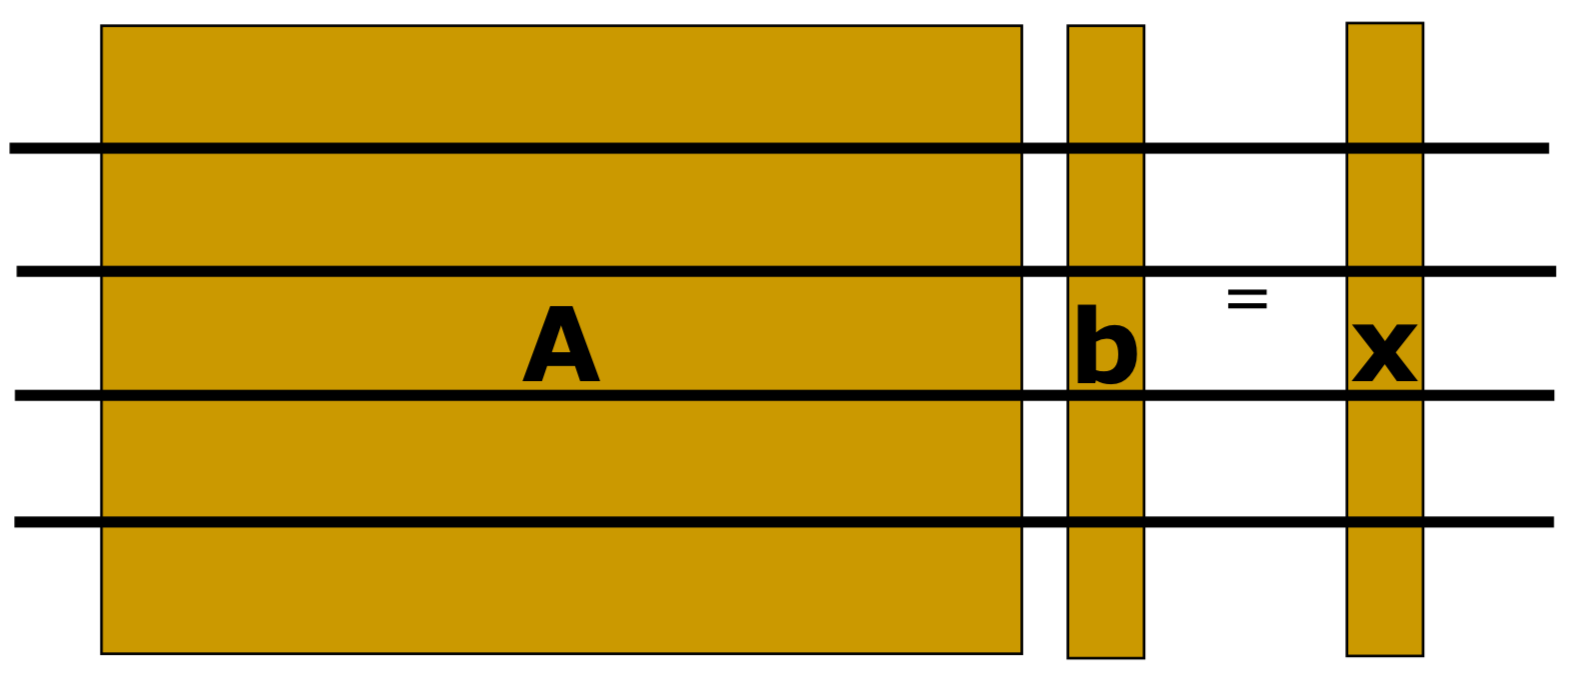
\includegraphics[width=0.5\linewidth]{images/Row-wise.png}
    \caption{Row-wise Matrix-Vector Multiplication}
    \label{fig:row-wise}
\end{figure}
Note the following:

\begin{itemize}
    \item The matrix rows are already local to $P_i$, so no communication is needed for accessing the matrix.
    \item The corresponding output elements of $x$ that result from multiplying the local rows are also stored locally, and thus need not be communicated to other processes.
    \item However, the input vector $b$ is \textbf{distributed across all the processes}, so process $P_i$ only has access to a part of $b$. Therefore, each process must obtain the \textbf{entire} $b$ vector to perform its computation.
\end{itemize}

One solution is to use point-to-point communication primitives such as \texttt{MPI\_Send} and \texttt{MPI\_Recv}. Each process could, in a loop, send its part of the $b$ vector to all the other processes and receive the missing parts from them. While this is logically correct, it results in a verbose and cumbersome implementation.

Instead, observe the communication pattern here: all processes require \textbf{the same global data} — the full $b$ vector — which is initially distributed among them. This is a textbook use case for the \textbf{all-gather} communication pattern.

In \texttt{MPI\_Allgather}, each process contributes its piece of data (in this case, a chunk of the $b$ vector), and all processes collect the entire assembled vector. That is, all processes end up with the full $b$ vector. This makes \texttt{MPI\_Allgather} the ideal communication primitive for this scenario.

Thus, using \texttt{MPI\_Allgather}, the row-wise matrix-vector multiplication can be implemented efficiently and clearly in MPI.
\begin{lstlisting}[style=cppstyle]
MPI_Allgather(sendbuf, sendcount, sendtype, recvbuf, recvcount, recvtype, comm)
\end{lstlisting}

The entire communication pattern involving sending and receiving data between all processes can be captured using a single collective communication call — namely, \texttt{MPI\_Allgather}. Instead of writing a for loop of \texttt{MPI\_Send} and \texttt{MPI\_Recv} calls, each process now simply invokes a one-line function call with its local data. This local data can be a single element, an array, or even a matrix.
\begin{figure}[ht]
    \centering
    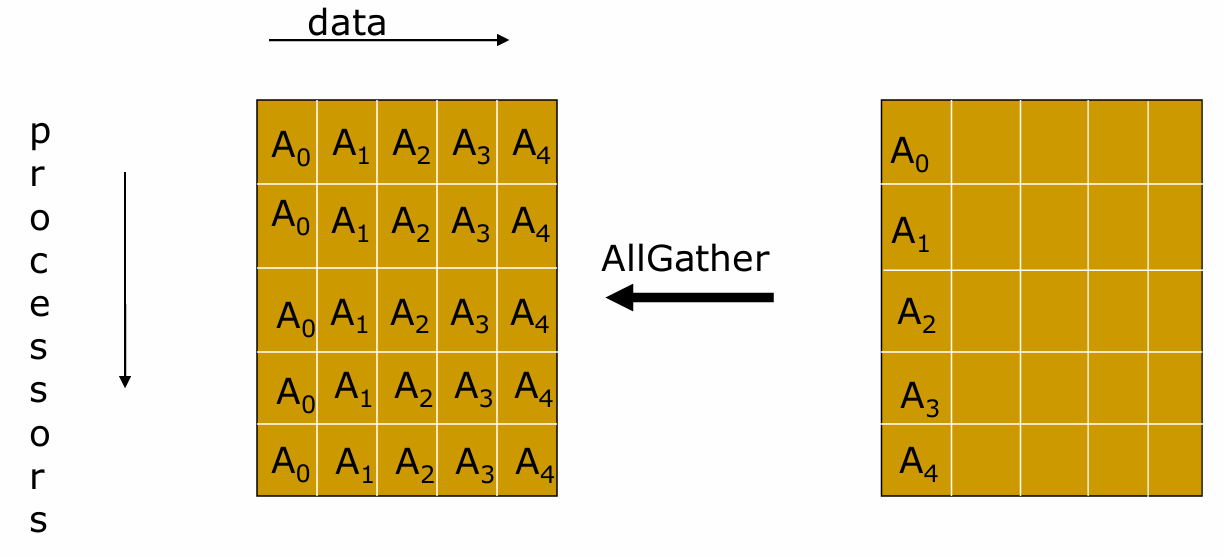
\includegraphics[width=0.75\linewidth]{images/all_gather.png}
    \caption{\texttt{MPI\_Allgather} operation}
    \label{fig:allgather}
\end{figure}
For example, process 0 may send its portion of the data (say, $A_0$) by filling the appropriate \texttt{sendbuf}, \texttt{sendcount}, and \texttt{sendtype}. Simultaneously, all processes will gather the full dataset into their local \texttt{recvbuf}, with corresponding \texttt{recvcount} and \texttt{recvtype}. Thus, all processes allocate a receive buffer, and after the \texttt{MPI\_Allgather} call, this buffer will contain the entire combined dataset from all processes. It is as shown in the figure~\ref{fig:allgather}. This function must be called by all processes that are part of the communicator \texttt{comm}, as it is a collective communication operation.

There is also a vector variant called \texttt{MPI\_Allgatherv}, which allows different processes to contribute different amounts of data:

\begin{lstlisting}[style=cppstyle]
MPI_Allgatherv(sendbuf, sendcount, sendtype, 
               recvbuf, recvcounts, displs, recvtype, comm);
\end{lstlisting}

Here, \texttt{recvcounts} is an array that specifies how much data each process contributes, and \texttt{displs} specifies where in the receive buffer each contribution should be placed.

Let us now consider an example using \texttt{MPI\_Allgather} to perform matrix-vector multiplication:

\begin{lstlisting}[style=cppstyle]
MPI_Comm_size(comm, &size);
MPI_Comm_rank(comm, &rank);
nlocal = n / size;

MPI_Allgather(local_b, nlocal, MPI_DOUBLE, b, nlocal, MPI_DOUBLE, comm);

for (i = 0; i < nlocal; i++) {
    x[i] = 0.0;
    for (j = 0; j < n; j++) {
        x[i] += a[i*n + j] * b[j];
    }
}
\end{lstlisting}

In this code:
\begin{itemize}
    \item Each process first determines the total number of processes (\texttt{size}) and its own rank (\texttt{rank}) in the communicator.
    \item The matrix $A$ is assumed to have $n$ total rows and is divided evenly among the processes, so each process works on $n_\text{local} = n / \texttt{size}$ rows.
    \item Each process possesses a local portion of the input vector $b$ (stored in \texttt{local\_b}) and needs the full vector $b$ to compute its portion of the result vector $x$.
    \item To achieve this, all processes perform a single \texttt{MPI\_Allgather} call to collect the full $b$ vector.
\end{itemize}

The final loop then performs the dot product between each local row of matrix $A$ and the global vector $b$, and stores the result in the local portion of $x$.

Using collective communication like \texttt{MPI\_Allgather} significantly reduces programming complexity. More importantly, it gives the MPI library knowledge of the global communication pattern, allowing it to choose an efficient communication algorithm optimized for the underlying architecture. In contrast, if only point-to-point communication (i.e., \texttt{MPI\_Send} and \texttt{MPI\_Recv}) is used, the MPI library cannot infer any global pattern and thus cannot optimize the communication strategy.

\textbf{Note:} The order in which data is stored in the receive buffer is based on process ranks. That is, data from process 0 appears first, followed by data from process 1, and so on.


\subsection{Reduce, AllReduce}

Suppose we now divide the matrix $A$ column-wise, such that the first set of columns resides in process $0$, the second set in process $1$, and so on. Since $b$ and $x$ are vectors, they are still divided row-wise as shown in figure~\ref{fig:column-wise}.
\begin{figure}[ht]
    \centering
    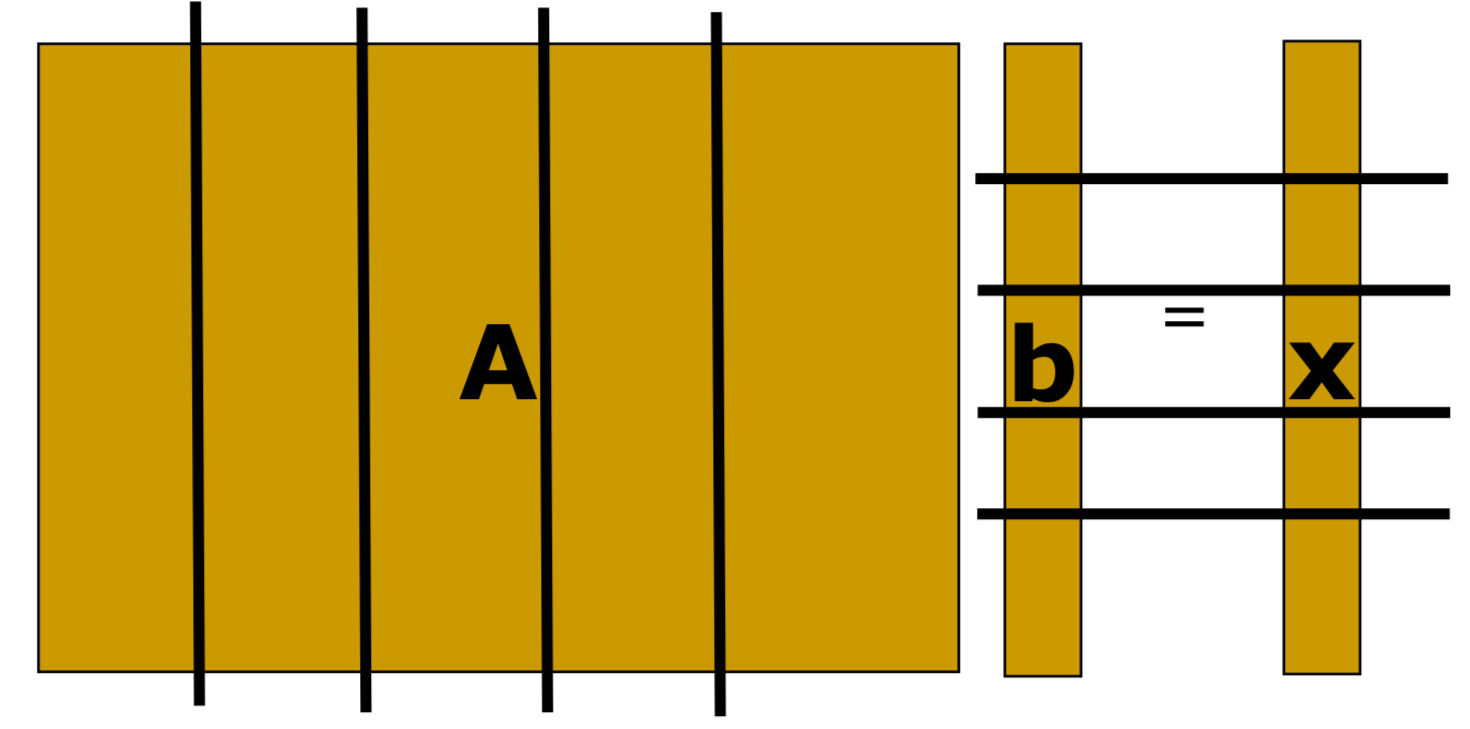
\includegraphics[width=0.5\linewidth]{images/Column-wise.png}
    \caption{Column-wise matrix-Vector Multiplication}
    \label{fig:column-wise}
\end{figure}
In this layout, the communication requirements change. For computing the inner product (i.e., matrix-vector multiplication), each processor already owns the portion of vector $b$ corresponding to the local columns of matrix $A$. Therefore, \textbf{no communication is required beforehand} — each process can compute its local contribution to the final result independently.

However, once local computations are complete, communication is required to \textbf{aggregate} these local results. Each processor computes a partial result (a local vector), and these must be \textbf{summed across all processes} to obtain the final result vector $x$. This is an example of a \textbf{reduction} communication pattern, where all processes contribute values that are combined using some operator (e.g., sum, max, min), and the final result is stored in a particular process.

Here is the MPI-based implementation of this scheme:
\begin{lstlisting}[style=cppstyle]
MPI_Comm_size(comm, &size);
MPI_Comm_rank(comm, &rank);
nlocal = n / size;

/* Compute partial dot-products */
for (i = 0; i < n; i++) {
    px[i] = 0.0;
    for (j = 0; j < nlocal; j++) {
        px[i] += a[i * nlocal + j] * b[j];
    }
}
\end{lstlisting}

As we can see, each process computes its part of the dot product and stores it in the local vector \texttt{px}. No communication is needed in this step.

To aggregate the local vectors into the final result $x$, MPI provides collective reduction operations such as \texttt{MPI\_Reduce}:

\begin{lstlisting}[style=cppstyle]
MPI_Reduce(px, x, n, MPI_DOUBLE, MPI_SUM, 0, comm);
\end{lstlisting}

This function performs the following:
\begin{itemize}
    \item \texttt{px} is the local array being sent (partial result from each process).
    \item \texttt{x} is the receive buffer in the root process (rank 0 in this example), where the final result will be stored.
    \item \texttt{n} is the number of elements in the arrays.
    \item \texttt{MPI\_DOUBLE} specifies the data type.
    \item \texttt{MPI\_SUM} is the operation used to combine data — in this case, addition.
    \item \texttt{0} is the rank of the root process where the result is stored.
    \item \texttt{comm} is the communicator.
\end{itemize}

MPI also provides other predefined operations such as:
\begin{itemize}
    \item \texttt{MPI\_MAX} — for computing the maximum of corresponding elements,
    \item \texttt{MPI\_MIN} — for computing the minimum,
    \item \texttt{MPI\_PROD} — for product,
    \item and many more.
\end{itemize}

In addition, MPI allows users to define \textbf{custom reduction operations} using the \texttt{MPI\_Op\_create} interface. This gives the programmer flexibility to implement and register user-defined functions that operate element-wise on arrays and pass them as operators in collective calls like \texttt{MPI\_Reduce} or \texttt{MPI\_Allreduce}.

Column-wise decomposition simplifies the local computation of matrix-vector multiplication but requires a global reduction to finalize the result. MPI’s reduction operations such as \texttt{MPI\_Reduce} help implement this efficiently and scalably.

In certain situations, it is desirable for the result of a reduction operation to be made available to \textbf{all} participating processes, rather than just a single root process. In such cases, one uses the collective communication:

\begin{lstlisting}[style=cppstyle]
MPI_ALLREDUCE(sendbuf, recvbuf, count, datatype, op, comm)
\end{lstlisting}
Here, there is \textbf{no root process}, and the final reduced result is stored in the \texttt{recvbuf} of every process. This is especially useful in parallel applications where all processes need the final computed result (e.g., for norm calculations, convergence checks, etc.).


\section*{Reduce-Scatter}

Consider that we have $P=8$ processes (ranks $0$ to $7$). Each process initially holds $n$ elements. 
For example, process $0$ has $A_0, A_1, \ldots, A_7$, process $1$ has $B_0, B_1, \ldots, B_7$, and so on.

The goal of a \texttt{Reduce-Scatter} operation is to:
1. Perform a reduction (e.g., addition) across all processes for each element position, and
2. Distribute the final reduced result such that each process holds only its designated portion.

For a reduction using addition:
\[
\text{Final data on process }i = A_i + B_i + C_i + \cdots + H_i, \qquad \text{for } i=0,\ldots,7.
\]

MPI provides a dedicated call \texttt{MPI\_Reduce\_scatter} for this.
A naive approach would use:
- \texttt{MPI\_Reduce} to gather and reduce all data at one root ($O(\log_2 P)$ steps), followed by
- \texttt{MPI\_Scatter} to distribute it back ($O(\log_2 P)$ steps).

This takes in total:
\[
O(\log_2 P) + O(\log_2 P) = O(2 \log_2 P)
\]
steps.

However, with dedicated algorithms such as Rabenseifner's method, the same operation can be completed in
\[
O(\log_2 P)
\]
steps, saving a factor of two in communication rounds.


\subsection*{Recursive Halving Algorithm (for commutative operations)}

This algorithm is the mirror image of recursive doubling. It proceeds as follows:

\begin{enumerate}
  \item At each step, processes are paired at a certain distance. Initially, the distance is $P/2$, then $P/4$, and so on, halving each time.
  \item Each process splits its current data into two halves: one half it needs to keep and one half it sends to the partner.
  \item Both processes exchange the appropriate half, perform the reduction on the received data, and keep only the portion assigned to them.
  \item After $\log_2 P$ steps, each process ends up with its reduced portion.
\end{enumerate}

\paragraph{Example: $P=8$ processes}
Each process starts with $[x_0, x_1, x_2, x_3, x_4, x_5, x_6, x_7]$.
Let the reduction be element-wise addition.

\begin{enumerate}
  \item \textbf{Step 1 (distance = $P/2 = 4$):}
  \begin{itemize}
    \item Pair $(0,4), (1,5), (2,6), (3,7)$.
    \item Each process sends its upper half ($x_4..x_7$) or lower half depending on convention and receives the complementary half from its partner.
    \item Reduce the received data with the local half to keep only the half that belongs to this side.
  \end{itemize}

  \item \textbf{Step 2 (distance = $P/4 = 2$):}
  \begin{itemize}
    \item Pair $(0,2), (1,3), (4,6), (5,7)$.
    \item Each process splits its remaining half into quarters and exchanges the corresponding quarter.
    \item Reduce and keep the assigned quarter.
  \end{itemize}

  \item \textbf{Step 3 (distance = $P/8 = 1$):}
  \begin{itemize}
    \item Pair $(0,1), (2,3), (4,5), (6,7)$.
    \item Exchange the final eighth and reduce.
    \item Now, each process holds exactly one element: the globally reduced value for its index.
  \end{itemize}
\end{enumerate}

This process completes in $\log_2 8 = 3$ steps.


\subsection*{Recursive Doubling Algorithm (for non-commutative operations)}

For non-commutative operations (e.g., matrix multiplication where order matters), the above algorithm does not guarantee correct ordering. Instead, we use recursive doubling.

The idea:
\begin{enumerate}
  \item Each process initially holds its entire data.
  \item At step 1, it exchanges \emph{all data except what it needs for its final result} with the partner at distance 1 and performs the operation in the correct order.
  \item At step 2, it exchanges the remaining data (all except the part it keeps and the part already exchanged) with a partner at distance 2.
  \item At step 3, it exchanges the remaining data with a partner at distance 4, and so on.
  \item After $\log_2 P$ steps, each process retains only its correct reduced data.
\end{enumerate}

\paragraph{Example: $P=8$ processes}
Suppose the operation is non-commutative. In the first step:
\begin{itemize}
  \item Pair $(0,1), (2,3), (4,5), (6,7)$.
  \item Each process sends all data except its local portion to the partner.
  \item Combine in the correct order.
\end{itemize}

Next steps:
\begin{itemize}
  \item Step 2: Pair $(0,2), (1,3), (4,6), (5,7)$ and repeat with the remaining data.
  \item Step 3: Pair $(0,4), (1,5), (2,6), (3,7)$.
\end{itemize}

After $\log_2 8=3$ steps, each process holds its reduced segment with the correct order preserved.

\paragraph{Key Observation:}
For commutative operations, recursive halving is optimal and most efficient.
For non-commutative operations, recursive doubling ensures the order of operations is preserved.
Both achieve $O(\log_2 P)$ steps, but recursive halving requires less data transfer at each step for commutative cases.

\section*{ReduceScatter using Recursive Doubling and Recursive Halving}

Consider $P=8$ processes, numbered from $0$ to $7$. Each process initially holds $8$ data elements. For example:
\[
\text{Process } 0: (A_0,A_1,\ldots,A_7),\quad
\text{Process } 1: (B_0,B_1,\ldots,B_7),\quad \ldots,\quad
\text{Process } 7: (H_0,H_1,\ldots,H_7).
\]
The goal of \texttt{MPI\_Reduce\_scatter} is to both reduce the data across all processes and scatter the reduced segments so that:
\[
\text{Process } i:\; A_i + B_i + C_i + \cdots + H_i,\quad i=0,\ldots,7
\]
(for a reduction operation, here shown as addition).

\subsection*{Recursive Doubling (for Non-Commutative Operations)}
In non-commutative operations, the order of operands matters. Therefore, we must ensure that the reduction preserves the left-to-right order of processes. Recursive doubling works as follows:

\begin{enumerate}
    \item \textbf{Step 1: Neighbor Pairing.} All even-numbered processes $i$ communicate with $i+1$. Each even process sends its upper half (indices $4$--$7$) and receives the lower half ($0$--$3$) of its neighbor, while each odd process does the opposite. For example:
    \begin{itemize}
        \item Process $0$ receives $(B_0,B_1,B_2,B_3)$ from Process $1$, reduces them with its first half, and keeps $(A_0+B_0,\ldots,A_3+B_3,A_4,A_5,A_6,A_7)$.
        \item Process $1$ receives $(A_4,A_5,A_6,A_7)$ from Process $0$, reduces them with its second half, and keeps $(B_0,B_1,B_2,B_3,A_4+B_4,\ldots,A_7+B_7)$.
        \item Similarly, $(2,3)$, $(4,5)$, and $(6,7)$ pairs perform the same operation.
    \end{itemize}

    \item \textbf{Step 2: Doubling Distance.} Now each process communicates with a partner at distance $2$. Thus, $(0,2)$, $(1,3)$, $(4,6)$, and $(5,7)$ exchange data. Each process sends the half it does not need and receives the complementary half. After reduction, Process $0$ would have:
    \[
    (A_0+B_0+C_0+D_0,\;A_1+B_1+C_1+D_1,\ldots, A_3+B_3+C_3+D_3, A_4+B_4,\ldots,A_7+B_7).
    \]

    \item \textbf{Step 3: Continue Doubling.} Repeat this with partners at distance $4$ until only one segment remains per process. After $\log_2 P=3$ steps, each process holds its final reduced segment.
\end{enumerate}

Recursive doubling ensures correct operand ordering because each process progressively exchanges only the necessary segments, respecting the left-to-right reduction sequence.

\subsection*{Recursive Halving (for Commutative Operations)}
For commutative operations (e.g., addition, multiplication), the order of operands does not matter. We can use a more efficient variant, \textbf{recursive halving}, which avoids forming full intermediate results at each process.

\begin{enumerate}
    \item Initially, each process divides its data into two halves. Each process $i$ exchanges one half with the process $i+\frac{P}{2}$.
    \item Both processes perform the reduction on the received half.
    \item The distance is halved at each step: $\frac{P}{2},\frac{P}{4},\frac{P}{8},\ldots,1$.
    \item After $\log_2 P$ steps, each process holds its final segment.
\end{enumerate}

\subsection*{Comparison of Recursive Doubling and Halving}
\begin{itemize}
    \item \textbf{Operation Type:} Recursive doubling preserves strict operand order and is necessary for non-commutative reductions. Recursive halving is valid only for commutative reductions.
    \item \textbf{Intermediate Storage:} Recursive doubling temporarily forms partial results for each process at each step, whereas recursive halving only forms the necessary partial segments.
    \item \textbf{Complexity:} Both methods achieve $O(\log_2 P)$ communication steps, which is twice as fast as a naive \texttt{Reduce} followed by \texttt{Scatter} ($O(2\log_2 P)$).
\end{itemize}



\subsection{\texttt{Scatter}, \texttt{Scatterv}, \texttt{Gather}, \texttt{Gatherv}}
Another essential collective communication is the \texttt{MPI\_SCATTER} operation. In this pattern, a single process (typically rank 0) possesses a large buffer of data and wants to distribute \textbf{equal-sized chunks} of it to all processes in the communicator group.

\begin{lstlisting}[style=cppstyle]
MPI_SCATTER(sendbuf, sendcount, sendtype, recvbuf, recvcount, recvtype, root, comm)
\end{lstlisting}


All processes must call this function collectively. The root process provides the data to distribute in \texttt{sendbuf}, and each process receives its chunk in \texttt{recvbuf}. This operation is widely used during the initialization phase of parallel programs when data is to be distributed from a central source.

When the data to be distributed to each process is of \textbf{different sizes}, we use the more general variant:

\begin{lstlisting}[style=cppstyle]
MPI_SCATTERV(sendbuf, sendcounts, displs, sendtype, recvbuf, recvcount, recvtype, root, comm)
\end{lstlisting}

Here, \texttt{sendcounts} is an array indicating how many elements each process should receive, and \texttt{displs} gives the starting offset for each process in the \texttt{sendbuf}.

The \texttt{MPI\_GATHER} collective communication operation is similar to \texttt{MPI\_SCATTER}, but in the reverse direction. In this pattern, we want to gather data from all processes in the communication group into a single root process.

\begin{lstlisting}[style=cppstyle]
MPI_Gather(sendbuf, sendcount, sendtype, recvbuf, recvcount, recvtype, root, comm);
\end{lstlisting}

Here,
\begin{itemize}
    \item Each process sends \texttt{sendcount} elements from its \texttt{sendbuf} of type \texttt{sendtype}.
    \item The root process receives all the data in its \texttt{recvbuf}, expecting \texttt{recvcount} elements from each process, all of type \texttt{recvtype}.
    \item \texttt{root} is the rank of the process that gathers the data.
    \item All processes must call this function, but only the root process needs to provide valid \texttt{recvbuf}.
\end{itemize}

\vspace{1em}
The \texttt{MPI\_GATHERV} operation is a more flexible variant of \texttt{MPI\_GATHER}, where each process can send a different number of elements. This is particularly useful when the data sizes to be gathered from different processors are not uniform.

\begin{lstlisting}[style=cppstyle]
MPI_Gatherv(sendbuf, sendcount, sendtype, recvbuf, recvcounts, displs, recvtype, root, comm);
\end{lstlisting}

Here,
\begin{itemize}
    \item \texttt{recvcounts} is an array of integers specifying the number of elements expected from each process.
    \item \texttt{displs} is an array of displacements (i.e., starting indices in \texttt{recvbuf}) where data from each process should be placed.
    \item This allows variable-length contributions from each process to be gathered efficiently into the root's receive buffer.
\end{itemize}
\begin{figure}[ht]
    \centering
    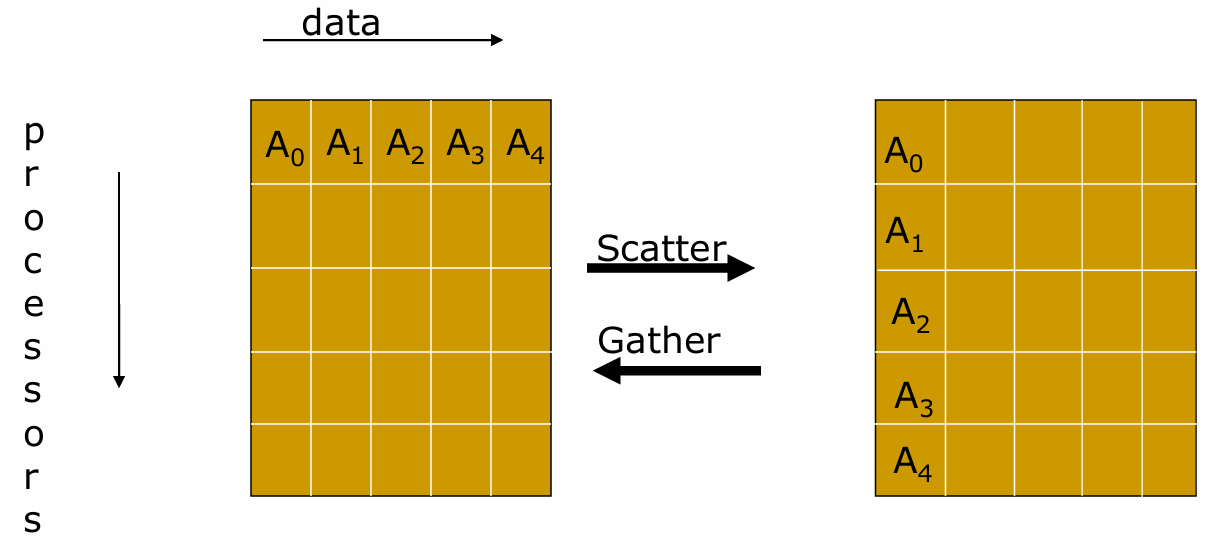
\includegraphics[width=0.75\linewidth]{images/scatter_gather.png}
    \caption{\texttt{Scatter} and \texttt{Gather} collective communication operations}
    \label{fig:scattergather}
\end{figure}

\vspace{1em}
Let us return to our example of column-wise matrix-vector multiplication. After all processes compute their local partial dot products and store them in \texttt{px}, we need to reduce them and distribute the final result. This can be achieved as follows:

\begin{lstlisting}[style=cppstyle]
/* Summing the dot-products */
MPI_Reduce(px, fx, n, MPI_DOUBLE, MPI_SUM, 0, comm);

/* Now all values of x are stored in process 0. 
   Need to scatter them to all processes */
MPI_Scatter(fx, nlocal, MPI_DOUBLE, x, nlocal, MPI_DOUBLE, 0, comm);
\end{lstlisting}

Here, we first use \texttt{MPI\_Reduce} to gather and sum all partial dot products into the buffer \texttt{fx} in process 0. Since we want the final vector $x$ to be distributed across all processes, we follow it up with a \texttt{MPI\_Scatter} to send $n_\text{local}$ values of $x$ to each process.

Alternatively, instead of gathering all values in process 0 and then redistributing them, we can use a clever method where each segment of the partial result \texttt{px} is reduced directly into the corresponding process:

\begin{lstlisting}[style=cppstyle]
for (i = 0; i < size; i++) {
    MPI_Reduce(px + i * nlocal, x, nlocal, MPI_DOUBLE, MPI_SUM, i, comm);
}
\end{lstlisting}

This results in each process directly receiving its portion of the reduced vector $x$, eliminating the need for an explicit scatter operation afterward.

\vspace{1em}
Collective communications offer two major advantages:
\begin{enumerate}
    \item \textbf{Reduced Programming Complexity:} Using one-line collective calls like \texttt{MPI\_Allreduce}, \texttt{MPI\_Scatter}, etc., avoids complex loops involving point-to-point communication.
    \item \textbf{Performance Optimization:} When using collective calls, the MPI library can detect communication patterns and apply optimized algorithms (such as tree-based or ring-based communication) for better efficiency. In contrast, such optimization is not possible with arbitrary combinations of \texttt{MPI\_Send} and \texttt{MPI\_Recv}.
\end{enumerate}

Up until \textbf{MPI-2}, only \textbf{blocking collective communication} routines were available. Starting from \textbf{MPI-3}, MPI introduced \textbf{non-blocking collective communication} routines. These behave similarly to their point-to-point counterparts like \texttt{MPI\_Isend} and \texttt{MPI\_Irecv}, allowing the program to initiate a communication and proceed with computation before explicitly waiting for its completion.

Just as \texttt{MPI\_Reduce} is used for a blocking reduction, we can now use:
\begin{center}
    \texttt{MPI\_Ireduce(..., \&request)}
\end{center}
to perform a non-blocking reduction, where \texttt{request} is an \texttt{MPI\_Request} object that can later be passed to \texttt{MPI\_Wait} or \texttt{MPI\_Test} to complete the communication.

Note the following important characteristics:
\begin{itemize}
    \item Non-blocking collectives in MPI-3 support only the \textbf{standard mode} of communication. Unlike point-to-point routines, \textbf{buffered}, \textbf{synchronous}, or \textbf{ready} modes are \textit{not supported} for collective routines.
    \item There is \textbf{no need for message tags} in collective communication. In point-to-point communication, message tags are used to provide scope or context to distinguish between multiple messages. However, collective operations are inherently well-scoped and synchronized across the communicator group. Therefore, the scope is implicit and tags are unnecessary.
\end{itemize}

\vspace{1em}

We also observed that many collective communication routines have both a \textbf{simple variant} (where equal-sized data is involved for all processes) and a \textbf{vector variant} (where data sizes may differ across processes). For example:
\begin{itemize}
    \item \texttt{MPI\_Allgather} and \texttt{MPI\_Allgatherv}
    \item \texttt{MPI\_Scatter} and \texttt{MPI\_Scatterv}
    \item \texttt{MPI\_Gatherv}, \texttt{MPI\_Reduce\_scatter}, etc.
\end{itemize}

Further, it is important to distinguish between routines that require a \textbf{root process} and those that do not:
\begin{itemize}
    \item Collectives like \texttt{MPI\_Scatter}, \texttt{MPI\_Gather}, and \texttt{MPI\_Reduce} require a \texttt{root} process argument, which acts as the sender or receiver of data.
    \item On the other hand, collectives like \texttt{MPI\_Allgather}, \texttt{MPI\_Allreduce}, and \texttt{MPI\_Bcast} do \textbf{not require} a root argument—they involve all processes equally.
\end{itemize}

\vspace{1em}

\textbf{Communication Pattern Classification:}
\begin{itemize}
    \item \textbf{One-to-all:} A single process sends data to all others. \\
        \textit{Example:} \texttt{MPI\_Bcast}, \texttt{MPI\_Scatter}
    \item \textbf{All-to-one:} All processes send data to one process. \\
        \textit{Example:} \texttt{MPI\_Reduce}, \texttt{MPI\_Gather}
    \item \textbf{All-to-all:} Every process sends and receives data from every other process. \\
        \textit{Example:} \texttt{MPI\_Allgather}, \texttt{MPI\_Allreduce}, \texttt{MPI\_Alltoall}
\end{itemize}

This classification helps in identifying the nature of communication and optimizing the parallel program based on the data flow requirement.

\subsection{Barrier}

We have already encountered the utility of barriers in earlier examples, particularly in the context of the grid solver, where synchronization between iterations was crucial. The \texttt{MPI\_Barrier} function provides a mechanism to ensure that all processes in a communicator reach a common synchronization point before any of them can proceed further. This is especially useful in iterative algorithms where the correctness of the next iteration depends on the completion of the previous one.
 
When a process calls \texttt{MPI\_Barrier}, it will be blocked until all other processes in the communicator have also called \texttt{MPI\_Barrier}. Once all processes have reached this point, they are released simultaneously. This ensures coordinated progress across all processes.

\paragraph{Implementing a Barrier using Point-to-Point Communication}  
Even though MPI provides \texttt{MPI\_Barrier} as a collective operation, it's important to note that any collective communication can, in principle, be implemented using point-to-point primitives like \texttt{MPI\_Send} and \texttt{MPI\_Recv}.

One naïve way to implement a barrier might be as follows:
\begin{itemize}
    \item Process $P_0$ sends a "finished" message to $P_1$.
    \item $P_1$ receives this message, performs its barrier work, then sends a message to $P_2$, and so on.
    \item Eventually, $P_{n-1}$ receives from $P_{n-2}$, completes its work, and then sends an acknowledgment message back to all the previous processes.
\end{itemize}
This approach involves $n - 1$ forward messages and $n - 1$ backward acknowledgments, resulting in $2(n - 1)$ sequential point-to-point communications.

\paragraph{Time Complexity:}  
The time complexity of this naïve linear chain barrier is $\mathcal{O}(n)$, where $n$ is the number of processes. This becomes a performance bottleneck for large-scale parallel programs.

\paragraph{Can We Do Better? Butterfly Barrier (Eugene Brooks)}  
Yes—we can reduce the time complexity from $\mathcal{O}(n)$ to $\mathcal{O}(\log_2 n)$ using a communication pattern called the \textbf{Butterfly Barrier}, proposed by Eugene Brooks.

This algorithm leverages the fact that $\log_2 n$ rounds of pairwise exchanges are sufficient for all processes to share synchronization status. In each round $r$, every process communicates with a partner process determined by flipping the $r$-th least significant bit of its rank. After $\log_2 n$ such rounds, all processes are guaranteed to have participated in a global barrier.

We will describe and illustrate this butterfly pattern in detail in the next subsection.
\subsubsection*{Butterfly Barrier Implementation}\label{subsec:butterfly}

The butterfly barrier algorithm was proposed by Eugene Brooks II and is a classic example of an efficient synchronization method. For $n$ processes, it requires at most $\mathcal{O}(2\log_2 n)$ pairwise synchronizations in the worst case. This approach was originally designed for shared-memory multiprocessors but is widely applicable due to its scalability and simplicity.

\paragraph{Algorithm Idea:}  
The core idea is that in each round $k$, process $i$ synchronizes with process $i \oplus 2^k$, where $\oplus$ denotes the bitwise XOR operation. The algorithm proceeds in $\log_2 n$ rounds, with each round doubling the number of processes each participant is aware of having synchronized.

Let us consider an example with $n = 8$ processes (numbered $0$ through $7$). The synchronization proceeds as follows:

\begin{itemize}
    \item \textbf{Stage 0:} Each process $i$ synchronizes with $i \oplus 1$. This forms the pairs (0,1), (2,3), (4,5), and (6,7).
    \item \textbf{Stage 1:} Each process $i$ synchronizes with $i \oplus 2$. Now, we get (0,2), (1,3), (4,6), and (5,7).
    \item \textbf{Stage 2:} Each process $i$ synchronizes with $i \oplus 4$. This leads to (0,4), (1,5), (2,6), and (3,7).
\end{itemize}

At the end of each round, the synchronization knowledge propagates exponentially. For example, by the end of Stage 1, process 5 has directly synchronized with 4 and 7 and indirectly with 6 (via 7). By the end of Stage 2, every process has synchronized—directly or transitively—with all others. Therefore, for $n=8$ processes, the barrier completes in $\log_2 8 = 3$ stages.

\begin{figure}[ht]
    \centering
    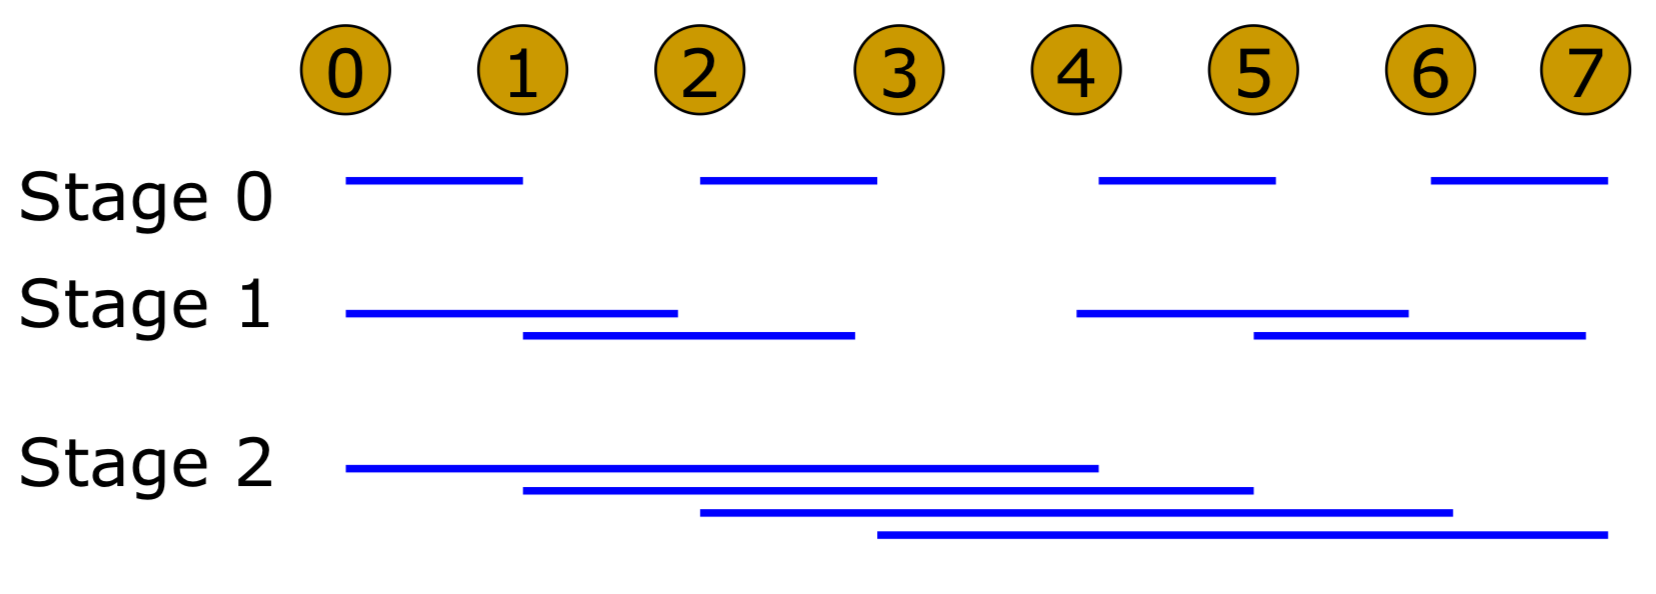
\includegraphics[width=0.6\linewidth]{images/Butterfly_barrier.png}
    \caption{Butterfly barrier implementation for 8 processes}
    \label{fig:butterfuly_barrier}
\end{figure}

\paragraph{Shared Memory Implementation:}  
In the original shared-memory setting, explicit communication was replaced by shared flags. For instance, process 0 sets a flag to indicate it has reached the barrier. Process 1, upon reading this flag, knows process 0 is ready, and vice versa. This read/write pattern continues in the butterfly shape across rounds, hence the name.

\paragraph{Non-Power-of-Two Case:}  
The algorithm works optimally when $n$ is a power of two. However, if $n$ is not a power of two, we can emulate a power-of-two barrier by using the next higher power of two and assigning some processes to play the role of ``dummy" partners. This leads to redundant communications and, in the worst case, increases the number of pairwise synchronizations to $\mathcal{O}(2\log_2 n)$. In case the number of processes is a non power of $2$, make virtual processes out of the existing processes to make up for the next power of $2$. So suppose we have 12 processes among which we were required to have a barrier implementation. The first step is to use processes $0,1,2,3$ as virtual processes to make up for the next power of $2$ i.e. $16$. So the communications occur in the same way where the communications between the virtual processes are mimicked by the processes that take its place. This results in repeated redundant communications to keep the algorithm logic simple. This leads to increase in the number of communications and in the worst case requires $2\log_2 P$ pairwise synchronizations by a processor.

The butterfly barrier is efficient, scalable, and well-suited to high-performance parallel computing systems. Compared to the naïve linear chain barrier (which takes $\mathcal{O}(n)$ time), the butterfly barrier reduces synchronization complexity to $\mathcal{O}(\log_2 n)$—a significant improvement for large-scale systems. 





\subsection{Broadcast}

Another important collective communication operation in MPI is \textbf{broadcast}. In a broadcast operation, a single process (called the \textbf{root}) sends the same piece of data to all other processes within the communicator. This is often used in parallel programs when one process has input data that needs to be shared with all other processes before computation begins.

MPI provides a standard interface for broadcast:

\begin{lstlisting}
MPI_BCAST(buffer, count, datatype, root, comm)    
\end{lstlisting}

\begin{itemize}
    \item \texttt{buffer}: The starting address of the data to be broadcast.
    \item \texttt{count}: Number of elements to broadcast.
    \item \texttt{datatype}: MPI datatype of the data.
    \item \texttt{root}: Rank of the process broadcasting the data.
    \item \texttt{comm}: Communicator involving all participating processes.
\end{itemize}

All processes in the communicator must call \texttt{MPI\_BCAST}, regardless of whether they are the root or a receiver.

\vspace{1em}
Although a naïve implementation would simply have the root process send the data individually to each of the $P - 1$ processes (which takes $\mathcal{O}(P)$ time), this is inefficient for large $P$. Instead, optimized implementations use a tree-based approach where communication happens in a hierarchical, staged fashion.

For example, using a binary tree scheme:
\begin{itemize}
    \item In the first step, the root sends data to two processes.
    \item In the second step, those two send to two more, and so on.
\end{itemize}
This results in a time complexity of $\mathcal{O}(\log_2 P)$ and significantly improves scalability.

MPI implementations typically use variations of binomial or pipeline trees for high efficiency, especially on large systems.

\vspace{1em}
\textbf{Important Notes:}
\begin{itemize}
    \item All processes must participate in the broadcast for it to succeed.
    \item The function is \emph{synchronous}, in the sense that all processes wait for the operation to complete before proceeding.
    \item Unlike point-to-point communication, there is no need for tags in collective communications. The scope and context are implied by the collective function itself.
\end{itemize}

\subsection{All-to-All}
\subsubsection*{\texttt{Allgather}}
This operation is somewhat similar to \texttt{MPI\_Allgather}, but with a key difference. In \texttt{MPI\_Allgather}, each process sends data that is broadcast to all other processes, and all processes receive the same global result. However, in \texttt{MPI\_Alltoall}, each process sends distinct data to every other process, and similarly receives distinct data from every other process. Thus, each process ends up with a unique collection of data from all other processes.

This pattern is particularly useful in scenarios where a distributed matrix needs to be transposed across processes, or when each process has some unique data for every other process. The result of this operation is conceptually equivalent to a transpose of a communication matrix. This is shown in figure~\ref{fig:alltoall}, where each process has multiple data items, each destined for a different target.

\begin{lstlisting}[style=cppstyle]
MPI_Alltoall(sendbuf, sendcount, sendtype,
             recvbuf, recvcount, recvtype, comm)
\end{lstlisting}

The vector variant of this communication, where different amounts of data are sent to different processes, is:

\begin{lstlisting}[style=cppstyle]
MPI_Alltoallv(sendbuf, array_of_sendcounts, array_of_displs, sendtype,
              recvbuf, array_of_recvcounts, array_of_displs, recvtype, comm)
\end{lstlisting}

Note that unlike collectives such as \texttt{MPI\_Bcast} or \texttt{MPI\_Reduce}, it is not possible to implement \texttt{MPI\_Alltoall} with $\mathcal{O}(\log_2 P)$ complexity. This is because each process must send a distinct message to every other process, which fundamentally requires $\mathcal{O}(P)$ communications.

\vspace{1em}
\begin{figure}[H]
    \centering
    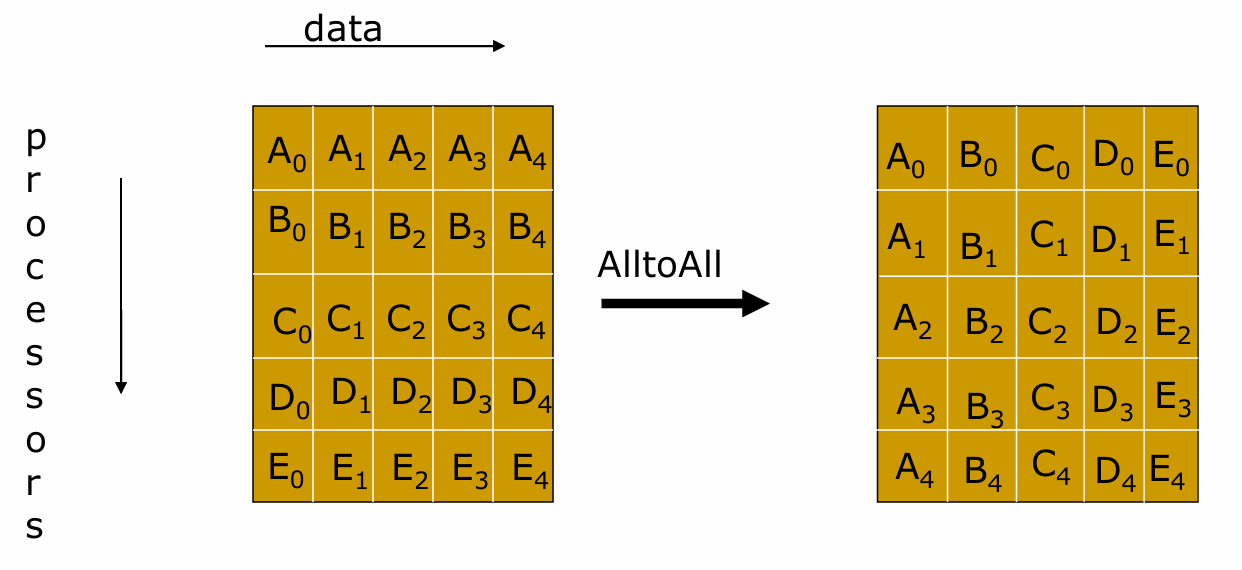
\includegraphics[width=0.65\linewidth]{images/alltoall.png}
    \caption{Schematic representation of All-to-All communication pattern}
    \label{fig:alltoall}
\end{figure}
\subsubsection{Example of Ring-based \texttt{Allgather} Strategy:}\label{subsubsec:allgatherring}
In general, the efficiency of collective operations like \texttt{Allgather}, \texttt{Alltoall}, and \texttt{Scan} heavily depends on the hardware topology, communication latency, and network contention.

As an example, suppose we implement a ring-based \texttt{Allgather} operation. The idea is that in each stage, every process sends data to its right neighbor and receives data from its left neighbor. This process continues for $p - 1$ steps if there are $p$ processes, resulting in an $\mathcal{O}(p)$ time complexity.
At stage 0:
\begin{itemize}
    \item Process 0 sends its data $A_0$ to Process 1.
    \item Process 1 sends its data $A_1$ to Process 2, and so on.
\end{itemize}

At the end of stage 0:
\begin{itemize}
    \item Each process $P_i$ now holds $A_i$ and $A_{i-1}$ (modulo $p$).
\end{itemize}

At stage 1:
\begin{itemize}
    \item Each process sends what it received in the previous stage to its right neighbor.
\end{itemize}

This continues until all $n$ pieces of data are circulated around the ring. Hence, it takes $O(p)$ stages. This is as shown in figure~\ref{fig:allgather_examp}.
\begin{figure}[ht]
    \centering
    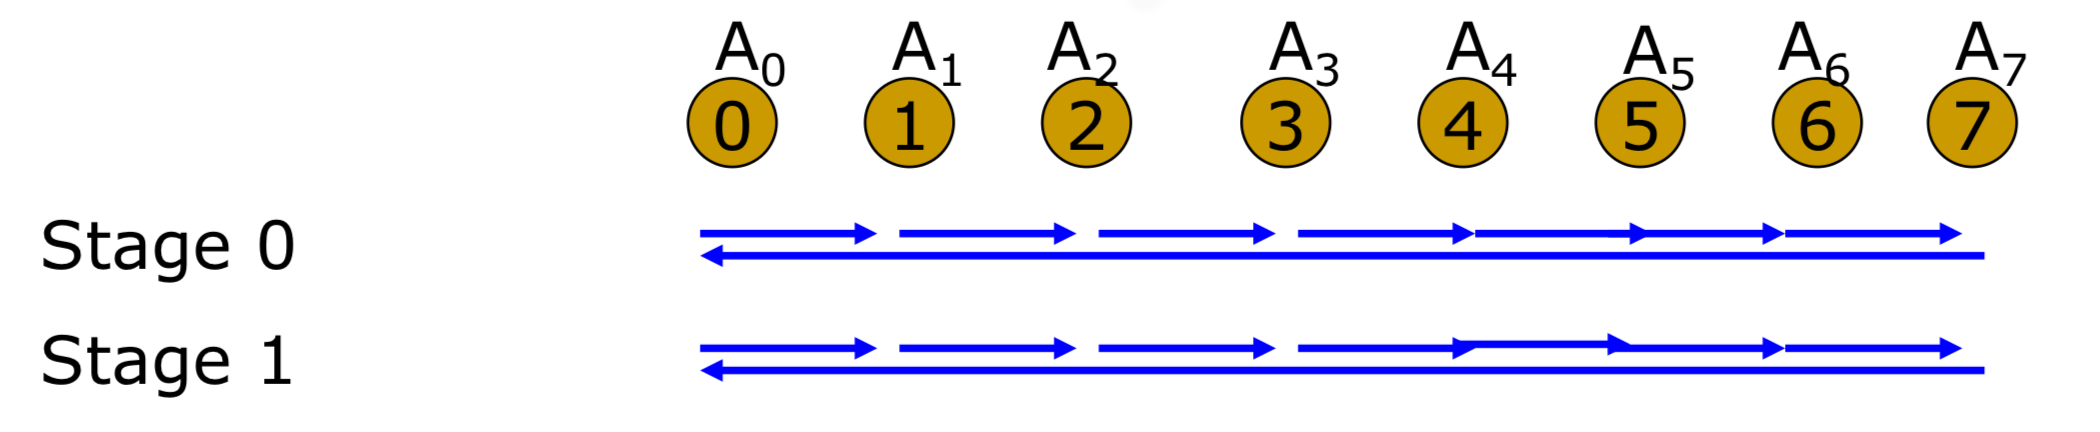
\includegraphics[width=0.75\linewidth]{images/allgather_examp.png}
    \caption{All gather operation for a ring-based topology}
    \label{fig:allgather_examp}
\end{figure} 

\subsection{\texttt{ReduceScatter}, \texttt{Scan}}

The idea behind \texttt{MPI\_Reduce\_scatter} is to first perform a reduction across all processes and then scatter the results among the processes, as illustrated in Figure~\ref{fig:reducescatter}. This collective operation combines the functionalities of both \texttt{MPI\_Reduce} and \texttt{MPI\_Scatter}.

\begin{lstlisting}[style=cppstyle]
MPI_Reduce_scatter(sendbuf, recvbuf,
                   array_of_recvcounts, datatype, op, comm);
\end{lstlisting}

The \texttt{MPI\_Scan} operation is known as a prefix sum or partial reduction operation. Unlike \texttt{MPI\_Reduce}, where the final result is available at a single process, in \texttt{MPI\_Scan}, each process receives the result of combining its data with the data from all lower-ranked processes. This is also called an \textbf{inclusive scan} or \textbf{inclusive prefix sum}. The behavior is illustrated in Figure~\ref{fig:scan}.

\begin{lstlisting}[style=cppstyle]
MPI_Scan(sendbuf, recvbuf, count,
         datatype, op, comm);
\end{lstlisting}

For example:
\begin{itemize}
    \item Process 0 has no prior process, so its result remains unchanged.
    \item Process 1 receives the combination (according to the given operator) of process 0 and process 1's data.
    \item Process 2 receives the combined result of processes 0, 1, and 2, and so on.
\end{itemize}

These kinds of operations are useful in many distributed algorithms, particularly in numerical computations, parallel prefix algorithms, and histogram computations.

\begin{figure}[H]
    \centering
    \includegraphics[width=0.75\linewidth]{images/reducescatter.png}
    \caption{Conceptual diagram of \texttt{MPI\_Reduce\_scatter}}
    \label{fig:reducescatter}
\end{figure}

\begin{figure}[H]
    \centering
    \includegraphics[width=0.75\linewidth]{images/scan.png}
    \caption{Inclusive prefix sum using \texttt{MPI\_Scan}}
    \label{fig:scan}
\end{figure}

\section{Collective Communication Implementations}
In this section, we explore generic algorithms whose primary purpose is to optimize the number of communication steps in collective communication. Later, we will also discuss the metrics to consider based on the underlying network topology used to implement the communication.

We begin by understanding how collective calls such as \texttt{MPI\_Bcast}, \texttt{MPI\_Scatter}, etc., work behind the scenes in the MPI library. The simplest, naive way to implement collective communication is through a \textit{flat tree}. In this approach, the root processor sends data to all other processors using point-to-point communication (\texttt{MPI\_Send}) within a loop. This approach results in a total of $O(p)$ communication steps, where each step involves sending data to one processor $P_i$.

However, this is not efficient, and we aim to reduce the number of communication steps to $O(\log p)$. The idea is to use a \textit{binary tree}. For example, consider $p=8$ processors, labeled from $P_0$ to $P_7$. The communication proceeds as follows:
\begin{itemize}
    \item Step 1: $P_0$ sends data to $P_1$.
    \item Step 2: $P_0$ sends data to $P_2$, and $P_1$ sends data to $P_3$.
    \item Step 3: $P_0$ sends data to $P_4$, $P_1$ sends data to $P_5$, and $P_2$ sends data to $P_6$.
    \item Step 4: $P_3$ sends data to $P_7$.
\end{itemize}
Thus, the total number of communication steps is proportional to $O(\log_2 p)$. 

While this binary tree method significantly improves over the flat tree, many MPI libraries use \textit{binomial trees} to further optimize the process. Binomial trees not only ensure a communication depth of exactly $\log_2 p$ when the number of processors is a power of two, but they also allow for better balancing of communication across processors.

\subsection*{Binomial Trees}
\textbf{Definition:} The binomial tree of order $k \geq 0$ with root $R$ is denoted as $B_k$ and is defined as follows:
\begin{enumerate}
    \item If $k=0$, then $B_k = \{R\}$; i.e., the binomial tree of order zero consists of a single node $R$.
    \item If $k>0$, then 
    \[
    B_k = \{R, B_0, B_1, \ldots, B_{k-1}\},
    \]
    i.e., the binomial tree of order $k>0$ comprises the root $R$, and $k$ binomial subtrees: $B_0, B_1, \ldots, B_{k-1}$.
\end{enumerate}

Each $B_k$ contains $2^k$ nodes, and the height of $B_k$ is $k$. The number of nodes at level $l$ in $B_k$, where $0 \leq l \leq k$, is given by the binomial coefficient:
\[
\binom{k}{l}.
\]

\begin{figure}
    \centering
    \includegraphics[width=0.75\linewidth]{images/binomial_trees.png}
    \caption{Binomial Trees}
    \label{fig:binom_trees}
\end{figure}
This structure is illustrated in Figure~\ref{fig:binom_trees}. Using binomial trees ensures that the communication depth is exactly $\log_2 p$ when the number of processors is a power of two, and it typically provides better load balancing than a simple binary tree.

% Example figure placeholder
\begin{figure}[H]
    \centering
    \includegraphics[width=0.75\textwidth]{images/binomial_tree_example.png}
    \caption{An example of a binomial tree $B_k$ for $k=4$.}
    \label{fig:binomial_tree}
\end{figure}

Broadcast, Scatter and Gather collective communications are usually implemented by binomial trees. using it takes exactly $\log_2 P$ communication steps instead of $2(\log_2 P -1)$ in binary trees. The communications works as follows. refer figure~\ref{fig:binomial_tree} for understanding communication in a binomial tree of $B_4$. At time step $0$ Process $0$ communicates with the rightmost child i.e. Process $8$. At the next time step Process $0$ will communicate with its next right most child i.e. Process $4$ and Process $8$ will also communicate with its right most child process $12$ and so on this continues in this pattern till all the processes have been communicated. Observe that in each step we are doubling the number of communications and this takes exactly $\log_2 P$ communications instead of $2(\log_2 P -1)$ communications.


\subsection{Barrier Algorithms}
\subsubsection{Dissemination Barrier}
Recall the Butterfly barrier implementation in subsection~\ref{subsec:butterfly}. Another efficient barrier implementation called Dissemination Barrier was proposed by Hensgen, Finkel, and Manser. The key idea is that in round $k$, process $i$ signals process 
\[
(i + 2^k) \bmod p.
\]
Unlike pairwise synchronization, this method does not require explicit pairwise coordination between specific processes in each round. The critical path length is at most 
\[
\log_2\bigl(\text{next power of } 2 > p\bigr),
\]
irrespective of the number of processes $p$.

The procedure operates as follows: at stage $k$, each process $i$ communicates with process $(i+2^k) \bmod p$. Processes for which $(i+2^k) \geq p$ simply wrap around due to the modulo operation, ensuring that every process always has a valid partner to communicate with. One of the problems with dissemination barrier is that it has a lot of traffic and it works the best in case where we have a ring like structure with periodicity.
\begin{figure}[ht]
    \centering
    \includegraphics[width=0.75\linewidth]{images/dissemination.png}
    \caption{Dissemination Barrier Example for $p=12$ processes}
    \label{fig:dissemination}
\end{figure}
This is illustrated in Figure~\ref{fig:dissemination}, where the dissemination pattern ensures logarithmic communication complexity.

\subsubsection{MPICH Barrier}
This barrier implementation is used in the open-source MPI library, MPICH. It employs a pairwise exchange algorithm with recursive doubling, similar to the butterfly barrier.

If the number of nodes is not a power of two, the algorithm first determines the nearest lower power of two:
\[
m = 2^{\lfloor \log_2(\text{size}) \rfloor}.
\]
The remaining nodes are called \emph{surfeit nodes}, with the count given by
\[
\text{surfeit} = \text{size} - m.
\]

The procedure is as follows:
\begin{enumerate}
    \item Each surfeit node initially sends its barrier message to a corresponding node among the first $m$ nodes.
    \item The first $m$ nodes then perform the recursive doubling (butterfly) barrier.
    \item Finally, the first $m$ nodes send completion messages back to their corresponding surfeit nodes.
\end{enumerate}

This approach allows MPICH to handle arbitrary numbers of processes efficiently, while ensuring that the core barrier is performed using a logarithmic number of communication steps for the largest power-of-two subset of processes. This takes $\lfloor \log_2 size\rfloor +2$ communication steps. For example, for a $12$ processes it is as demonstrated in the following figure~\ref{fig:MPICHbarrier}.
\begin{figure}
    \centering
    \includegraphics[width=0.75\linewidth]{images/MPICH.png}
    \caption{MPICH Barrier Implementation for $p=12$ processes}
    \label{fig:MPICHbarrier}
\end{figure}
Compared to the butterfly implementation, the MPICH barrier requires only 
\[
\lfloor \log_2 p \rfloor + 2
\]
communication steps, as opposed to $2\log_2 p$ steps in the butterfly barrier. 

When compared to the dissemination barrier, MPICH has slightly more communication steps but results in lower traffic per communication step. As one can observe, the communication pattern in the dissemination barrier resembles a ring network topology; hence, the dissemination barrier performs best on ring networks.

In general, the optimal barrier implementation depends on the underlying network topology. In the absence of such knowledge, one typically relies on comparing the number of communication steps to select the most efficient barrier.

\subsubsection{Tournament Barrier}

The \textit{tournament barrier}, proposed by Hensgen, Finkel, and Manseer, organizes synchronization among processors in a tournament-style fashion.  

\textbf{Idea:}  
\begin{itemize}
    \item In the first round, each pair of processors (players) synchronize with each other (play a ``match'').
    \item In each match, one processor is designated as the \textit{receiver}, and this processor is considered the winner of the round.
    \item In the second round, the winners from the first round synchronize with each other, with the receivers advancing to the next round.
    \item This process continues until only one winner remains at the top of the tournament.
    \item The single winner then broadcasts a release message to all other processors, allowing them to continue.
\end{itemize}

At each round $k$, processor $j$ receives a message from processor
\[
i = j - 2^k,
\]
as shown in Figure~\ref{fig:tourbar}. This ensures a logarithmic number of rounds for synchronization.

\begin{figure}[ht]
    \centering
    \includegraphics[width=0.5\linewidth]{images/tournamentselc.png}
    \caption{Tournament barrier: processors synchronize in rounds until a single winner remains, who then broadcasts a release signal.}
    \label{fig:tourbar}
\end{figure}


For further details refer sections 5.1 from~\cite{quinn1994parallel}.
\subsection{Allgather Implementations}
\subsubsection{Bruck's Allgather}

Recall ring-based all gather implementation~\ref{subsubsec:allgatherring}. This algorithm follows a communication pattern similar to the dissemination barrier. At each communication step, each processor shares all the information it has with another processor following the same pattern as in the dissemination barrier. 
Hence, the algorithm requires 
\[
O(\log_2 p)
\]
communication steps, in contrast to the 
\[
O(p)
\]
steps required in a naive ring-based allgather.

However, it is important to note that for a ring network topology, the traditional ring-based allgather can work very efficiently because it fully utilizes the direct connections of the ring, even though it involves more communication steps 
than Bruck's algorithm. Here, we are required to have higher communication hops leading to more traffic as opposed to only near neighbor communication in the ring-based allgather and hence the underlying topology plays very important role.

\subsection{AlltoAll Implementations}
\textbf{Naïve vs Optimized Communication Pattern:}

A naïve implementation might look like the following:

\begin{lstlisting}[style=cppstyle]
// Naive All-to-All (sequential and bottlenecked)
for all processes i in order {
    if (i != my_proc) {
        send to process i;
        receive from process i;
    }
}
\end{lstlisting}

This approach introduces serialization and communication hotspots due to synchronization around a fixed global order. A better strategy is to ``break symmetry" and have each process follow its own order in a round-robin fashion (MPICH Implementation). This avoids bottlenecks and maximizes parallelism:

\begin{lstlisting}[style=cppstyle]
// Optimized All-to-All using ring pattern
for (i = 0; i < P; i++) {
    dest = (my_proc + i) % P;
    src  = (my_proc - i + P) % P;
    send to dest;
    receive from src;
}
\end{lstlisting}

This circular scheduling pattern ensures full utilization of communication links and avoids contention, making the operation significantly faster on large systems.

\subsubsection{Circular AlltoAll}
For steps $k$ i ${1,\ldots,P}$ processor $i$ sends to $(i+k) \mod P$ and receives from $(i-k+P)\mod P$ as shown in figure~\ref{fig:circalltoall}.
\begin{figure}
    \centering
    \includegraphics[width=0.5\linewidth]{images/circalltoall.png}
    \caption{Circular All to All Implementation}
    \label{fig:circalltoall}
\end{figure}
\subsection{Reduce, AllReduce}

\subsubsection{Rabenseifner Algorithm}
We have previously seen binary tree (and even binomial tree) implementations for \texttt{reduce} 
and \texttt{gather}. Although these implementations perform well for \texttt{gather}, 
they are not as efficient for \texttt{reduce}. 

The reason is that \texttt{reduce} and \texttt{allreduce} operations involve both 
\emph{communication and computation}, whereas \texttt{gather} involves only communication. 
These operations can also include user-defined functions, which may involve performing 
computations on large arrays. 

In tree-based approaches, as we move higher up the tree, fewer processors remain 
active in performing these operations, while most of the processors stay idle. 
This results in poor load balancing, as only a small number of processors at the 
higher levels of the tree handle the computational burden.

To overcome this limitation, Rolf Rabenseifner of Stuttgart proposed an algorithm 
that ensures all processes are equally involved in both communication and computation 
for \texttt{reduce} and \texttt{allreduce}.

The algorithm is illustrated with an example using 13 nodes. 
The nodes are numbered from $0$ to $12$, and the send buffer contents 
are labeled as $a,b,c,\ldots,m$. Each buffer is conceptually divided 
into equal-sized segments. For example, if a buffer is denoted as 
``ABCDEFGH'', then ``C'' refers to the third $1/8$ of the buffer.

Let the variable \texttt{size} denote the number of nodes in the communicator, 
and let $2^n$ be the largest power of $2$ less than or equal to \texttt{size}. 
Define 
\[
r = \texttt{size} - 2^n.
\]
For instance, if $\texttt{size} = 13$, then $n=3$ and $r=5$. The algorithm proceeds as follows:
\begin{algorithm}[H]
\caption{Rabenseifner's Algorithm}
\label{alg:rabenseifner}
\begin{algorithmic}[1]
\State Compute $n$ and $r$, where $2^n$ is the largest power of two such that $2^n \leq \texttt{size}$, and set $r = \texttt{size} - 2^n$.
\If{\texttt{myrank} $< 2^n$}
    \State Split the buffer into two halves: \texttt{ABCD} (lower half) and \texttt{EFGH} (upper half).
    \If{\texttt{myrank} is even}
        \State Send buffer \texttt{EFGH} to $\texttt{myrank}+1$.
        \State Receive buffer \texttt{ABCD} from $\texttt{myrank}+1$.
        \State Perform reduction on \texttt{ABCD}.
        \State Receive reduced buffer \texttt{EFGH}.
    \Else \Comment{myrank is odd}
        \State Send buffer \texttt{ABCD} to $\texttt{myrank}-1$.
        \State Receive buffer \texttt{EFGH} from $\texttt{myrank}-1$.
        \State Perform reduction on \texttt{EFGH}.
        \State Send reduced buffer \texttt{EFGH} to $\texttt{myrank}-1$.
    \EndIf
\EndIf

\State Define new ranks:
\[
\text{NEWRANK}(\text{old}) =
\begin{cases}
\frac{\text{old}}{2}, & \text{if } \text{old}<2^n,\\
\text{old}-r, & \text{otherwise},
\end{cases}
\qquad
\text{OLDRANK}(\text{new}) =
\begin{cases}
2\times \text{new}, & \text{if } \text{new}<r,\\
\text{new}+r, & \text{otherwise}.
\end{cases}
\]

\State Perform recursive halving: at each step, split the remaining buffer and exchange data with a partner at distance $2^k$, for $k=0,1,\ldots,\log_2 P -1$.
\State The final step is a gather phase:
\begin{itemize}
    \item Gathering proceeds using a tournament-style algorithm.
    \item In each round, one process gathers data from another.
    \item The number of active processes starts at $P/2$ and is halved at each step until only one process remains.
\end{itemize}
\end{algorithmic}
\end{algorithm}

\paragraph{For $P=13$ ranks.}
Let \(\texttt{size}=13\). Let \(2^n\) be the largest power of two \(\le 13\), so \(2^n=8\) and \(r=\texttt{size}-2^n=5\).
Rabenseifner's method first \emph{folds} the extra \(r\) ranks into the first \(2^n\) ranks, then performs a power-of-two
\emph{reduce-scatter using recursive halving}, and finally, if an \texttt{Allreduce} is required, applies an \emph{allgather using recursive doubling}.
Below, we explain the initial folding and the first three stages of reduce-scatter.

\medskip
Assume each rank holds the same input buffer, conceptually divided into eight equal contiguous chunks:
\(\texttt{A B C D | E F G H}\).
We use addition \((+)\) as the reduction operator (any associative and commutative operator \(\oplus\) works the same).
For intuition, consider a single scalar from that buffer, with ranks \(0,1,\ldots,12\) contributing values \(a,b,\ldots,m\).

\begin{enumerate}
  \item \textbf{Folding to a power-of-two group.}
  The \(r=5\) surplus ranks \(8,9,10,11,12\) send their full buffers to ranks \(0,1,2,3,4\), respectively.
  These receivers immediately reduce (add) the received data into their local buffers.
  After this folding step, only ranks \(0\)–\(7\) remain active, each now representing the sum of two original ranks when applicable
  (e.g., rank \(0\) holds \(a+m\), rank \(1\) holds \(b+l\), etc.).
  No data is lost; the system is effectively reduced to a power-of-two size.

  \item \textbf{Recursive halving, stage \(k=0\) (partner distance \(2^0=1\); halves).}
  Pair ranks as \((0,1), (2,3), (4,5), (6,7)\).
  Each rank splits its buffer into a lower half (\(\texttt{ABCD}\)) and an upper half (\(\texttt{EFGH}\)).
  \begin{itemize}
    \item Even ranks send their upper half and receive the lower half, reducing it in place.
    \item Odd ranks send their lower half and receive the upper half, reducing it in place.
  \end{itemize}
  The explicit first exchange is:
  \[
    \texttt{ABCD: }\{1\!\to\!0,\;3\!\to\!2,\;5\!\to\!4,\;7\!\to\!6\}, \qquad
    \texttt{EFGH: }\{0\!\to\!1,\;2\!\to\!3,\;4\!\to\!5,\;6\!\to\!7\}.
  \]
  After this step, even ranks hold reduced \(\texttt{ABCD}\) and odd ranks hold reduced \(\texttt{EFGH}\).
  For illustration:
  \[
  \begin{aligned}
  \text{Node 0: } & (a+b)+(c+d), \quad
  \text{Node 1: } (a+b)+(c+d), \\
  \text{Node 2: } & (e+f)+(g+h), \quad
  \text{Node 3: } (e+f)+(g+h), \\
  \text{Node 4: } & (i+j)+k, \quad
  \text{Node 5: } (i+j)+k, \\
  \text{Node 6: } & l+m, \quad
  \text{Node 7: } l+m.
  \end{aligned}
  \]

  \item \textbf{Recursive halving, stage \(k=1\) (partner distance \(2^1=2\); quarters).}
  Each rank splits its retained half into two quarters:
  even ranks: \(\texttt{ABCD} \to \texttt{AB}|\texttt{CD}\),
  odd ranks: \(\texttt{EFGH} \to \texttt{EF}|\texttt{GH}\).
  Pairs: \((0,2),(1,3),(4,6),(5,7)\).
  Within each pair, the appropriate quarter is exchanged and reduced.
  For example, rank \(0\) keeps reduced \(\texttt{AB}\), rank \(2\) keeps reduced \(\texttt{CD}\); similarly for the others.

  \item \textbf{Recursive halving, stage \(k=2\) (partner distance \(2^2=4\); eighths).}
  Each remaining quarter is split into two eighths.
  Pairs: \((0,4),(1,5),(2,6),(3,7)\).
  Exchange and reduce the required eighth.
  After this step, each active rank holds exactly one distinct eighth of the fully reduced buffer
  (e.g., rank \(0\) holds reduced \(\texttt{A}\), rank \(1\) holds reduced \(\texttt{E}\), etc.,
  depending on the keep/send convention).
\end{enumerate}

\noindent
\textbf{What happens next?}
\begin{itemize}
  \item If the goal is a \emph{Reduce} to a root within the power-of-two group, the root gathers the eight reduced eighths
        (often by recursive doubling), and the folded-out ranks \(8\)–\(12\) are handled at the beginning/end as needed.
  \item If the goal is an \emph{Allreduce}, the standard continuation is an \emph{allgather by recursive doubling} over the same \(8\) ranks,
        which distributes all eight reduced eighths to every rank in \(\{0,\ldots,7\}\) in \(\log_2 8=3\) steps.
        Finally, results are sent back to the folded ranks \(8\)–\(12\) to complete the communicator.
\end{itemize}

\noindent
\textbf{Why the pattern repeats with \(2^k\)?}
At stage \(k\), partners are at distance \(2^k\), and the owned segment size halves each time.
After \(n=\log_2 8=3\) halving stages, ownership is \(1/8\) of the buffer, fully reduced.
This yields \(O(\log_2 P)\) communication steps on the critical path for the power-of-two core,
with balanced computation at each stage (each rank reduces the portion it keeps).

\subsection{Reduce-Scatter}

\subsubsection{Commutative Operations: Recursive Halving Algorithm}
The recursive halving algorithm can be seen as the reverse of recursive doubling.  
In the first step, each process communicates with another process at distance $P/2$.  
It sends the portion of data needed by the other half and receives the portion needed for its own half. After the exchange, each process performs the reduction operation on the received data.  

In the next step, the communication distance is halved to $P/4$, and the same process is repeated.  
This continues for $\log P$ steps until all processes hold the reduced result corresponding to their assigned portion.  

Because the operation is commutative, the order of application does not affect the correctness of the result.

\subsubsection{Non-Commutative Operations: Recursive Doubling Algorithm}
When the reduction operation is non-commutative, the recursive doubling algorithm is used to preserve the correct order.  

In the first step, each process exchanges its data (all except the portion it requires for its result) with its immediate neighbor.  
In the second step, each process exchanges the appropriate subset of data with a process at distance $2$.  
In the third step, the distance doubles again to $4$, and so on.  

At each step, the subset of data to be communicated decreases:  
\begin{itemize}
    \item Step 1: $(n - n/p)$ elements exchanged with neighbor at distance $1$.
    \item Step 2: $(n - 2n/p)$ elements exchanged with process at distance $2$.
    \item Step 3: $(n - 4n/p)$ elements exchanged with process at distance $4$.
    \item \dots
\end{itemize}

This continues for $\log P$ steps, after which each process has exactly the portion of the reduced data it is responsible for.  


For further details refer~\cite{thakur2005optimization}.

\subsection{Optimizing Collectives}
Collective communication performance is generally characterized by two main components: \textbf{latency} and \textbf{bandwidth}.
\begin{itemize}
    \item \textbf{Latency} ($\alpha$): The time required to initiate the communication and deliver the first byte. It is often expressed in terms of the number of time steps or the fixed overhead incurred regardless of the message size.
    \item \textbf{Bandwidth} ($\beta$): The rate at which data is transferred after the first byte has been sent. It determines the time taken for the remaining data to be communicated.
\end{itemize}

The total communication cost can be modeled as:
\[
T_\text{comm} = \alpha + n\beta,
\]
where $n$ is the number of bytes (or words) transmitted.

Latency dominates for small message sizes, where the startup overhead is significant, while bandwidth dominates for large message sizes, where the data transfer time becomes the limiting factor. Efficient collective algorithms aim to minimize both components depending on the communication pattern and data size.

\subsubsection*{Example: Broadcast Optimization}
Consider the broadcast operation where a root process sends a message of size $n$ to $p$ processes. There are two commonly used strategies:

\begin{itemize}
    \item \textbf{Binomial Broadcast:}  
    This method uses a binomial tree structure and takes $\log_2 p$ communication steps.  
    At each step, the full message of size $n$ is sent to the corresponding partner process in the tree.  
    Thus, the total communication cost is:
    \[
    T_\text{binomial} = \log_2 p \, (\alpha + n\beta),
    \]
    where $\alpha$ is the latency per message and $\beta$ is the cost per byte (or word) transferred.

    \item \textbf{Scatter + Allgather:}  
    In this approach, the message is first divided into $p$ segments of size $n/p$ each.  
    These segments are scattered to $p$ processes using a binomial scatter, costing:
    \[
    T_\text{scatter} = \log_2 p \, \alpha + \frac{n}{p}(p-1)\beta.
    \]
    Compared to previous approach where the entire data was sent to each of the processes. Irrespective of whether one uses binomial tree or flat tree to scatter the data. Here, after scattering, the segments are collected at all processes using a ring allgather, with a cost of:
    \[
    T_\text{allgather} = (p-1)\alpha + \frac{n}{p}(p-1)\beta.
    \]
    Therefore, the total cost of this strategy is:
    \[
    T_\text{scatter+allgather} = (\log_2 p + p - 1)\alpha + 2\frac{n}{p}(p-1)\beta.
    \]

\end{itemize}

For small messages, the binomial broadcast is generally more efficient due to its lower latency overhead.  
For large messages, the scatter + allgather approach performs better because the message is divided, reducing the per-step bandwidth cost.

\subsection{MPICH Algorithms}
Open-source MPI implementations such as MPICH do not rely on a single algorithm for a given collective operation. Instead, they select among multiple algorithms depending on the message size, the number of processes, and whether the operation is commutative or user-defined. Some examples are:

\begin{itemize}
    \item \textbf{Allgather:} 
    \begin{itemize}
        \item Bruck's algorithm (a variation of dissemination) for small messages ($<80$ KB) and non-power-of-two process counts.
        \item Recursive doubling for power-of-two process counts with message size $<512$ KB.
        \item Ring algorithm for large messages ($>512$ KB) and also for intermediate message sizes (80--512 KB) with any process count.
    \end{itemize}

    \item \textbf{Broadcast:} 
    \begin{itemize}
        \item Binomial tree algorithm for small messages ($<12$ KB).
        \item Binomial scatter combined with ring allgather for large messages ($>512$ KB).
    \end{itemize}

    \item \textbf{AlltoAll:} 
    \begin{itemize}
        \item Bruck's algorithm for very small messages ($<256$ bytes).
        \item Post all \texttt{Irecv}s and \texttt{Isend}s for medium-sized messages (256 bytes--32 KB).
        \item Pairwise exchange for long messages and power-of-two process counts. This takes $p-1$ steps, where in step $k$, process $i$ exchanges data with process $i \oplus k$ (bitwise XOR).
        \item For non-power-of-two process counts, in each step $k$, process $i$ sends data to $(i+k)$ and receives from $(i-k)$ (mod $p$).
    \end{itemize}

    \item \textbf{Reduce-Scatter:} 
    \begin{itemize}
        \item For commutative operations: Recursive halving for small messages ($<512$ KB), pairwise exchange for large messages ($>512$ KB; $p-1$ steps; process $(\text{rank}+i)$ at step $i$).
        \item For non-commutative operations: Recursive doubling for short messages ($<512$ bytes), pairwise exchange for larger ones ($>512$ bytes).
    \end{itemize}

    \item \textbf{Reduce:}
    \begin{itemize}
        \item For predefined operations: Binomial algorithm for short messages ($<2$ KB), Rabenseifner’s algorithm for longer ones ($>2$ KB).
        \item For user-defined operations: Binomial algorithm.
    \end{itemize}

    \item \textbf{AllReduce:}
    \begin{itemize}
        \item For predefined operations: Recursive doubling for short messages, Rabenseifner’s algorithm for long messages.
        \item For user-defined operations: Recursive doubling.
    \end{itemize}
\end{itemize}


\subsection{On Real Network Topologies}
In practice, collective communication performance depends not only on the algorithm itself but also on how processes are mapped onto the underlying network topology. Two communicating processes may be mapped onto processors that are more than one hop away, or multiple communication edges in the algorithm’s graph may map onto the same physical link, leading to contention.

For example, in Allgather we compared two algorithms: the ring-based algorithm (which takes $p$ steps) and Bruck's algorithm (which takes only $\log p$ steps). At first glance, Bruck’s algorithm seems superior due to fewer steps. However, if the underlying network is a ring topology, the ring-based algorithm matches the topology very well: all communication happens only between neighboring processors. In contrast, Bruck’s algorithm requires multi-hop communication between processors, which often leads to worse performance on a ring network despite fewer algorithmic steps.

This raises the broader question: \textit{how should one best map the communication patterns of algorithms to the underlying network topology}? This is often studied through the concept of graph embeddings.

\textbf{Dilation:}  
Let $\phi$ be a function that embeds a graph $G=(V,E)$ into another graph $G'=(V',E')$. The \textit{dilation} of the embedding is defined as:
\[
\text{dil}(\phi) = \max \{ \, \text{dist}(\phi(u), \phi(v)) \;|\; (u,v) \in E \,\},
\]
where $\text{dist}(x,y)$ denotes the shortest-path distance between nodes $x$ and $y$ in $G'$.

\medskip
\textbf{Example 1: Ring onto 2D Mesh.}  
A dilation-1 embedding of a ring into a 2D mesh is possible if the mesh has an even number of rows and/or columns. Figure~\ref{fig:2dmeshring} shows an example for a $4 \times 5$ mesh.

\begin{figure}[ht]
    \centering
    \includegraphics[width=0.5\linewidth]{images/2dmeshproj.png}
    \caption{Dilation-1 embedding of ring onto 2D mesh}
    \label{fig:2dmeshring}
\end{figure}

\medskip
\textbf{Example 2: Trees onto 2D Mesh.}  
A dilation-1 embedding exists for trees of height $\leq 3$ (Figure~\ref{fig:2dmeshtree}). However, for binary trees of height $>4$, such an embedding is impossible. This can be shown by comparing growth rates:  
\begin{itemize}
    \item In a 2D mesh, the total number of nodes reachable within $k$ hops of a given node is $2k^2 + k + 1$.
    \item In a binary tree of height $k$, the total number of nodes is $2^{k+1}-1$.
\end{itemize}
Clearly,
\[
2k^2 + k + 1 < 2^{k+1} - 1 \quad \text{for } k > 4,
\]
so dilation-1 embedding is not possible.

\begin{figure}[ht]
    \centering
    \includegraphics[width=0.5\linewidth]{images/2dmeshtree.png}
    \caption{Dilation-1 embedding of a height-3 tree onto 2D mesh}
    \label{fig:2dmeshtree}
\end{figure}

The standard practice for embedding a binary tree onto a 2D mesh is to use an \textit{H-tree embedding}. Figure~\ref{fig:treemesh} illustrates the embedding of a binary tree of height 4 onto a mesh.

\begin{figure}[ht]
    \centering
    \includegraphics[width=0.5\linewidth]{images/btreemesh.png}
    \caption{Binary tree of height 4 embedded onto a 2D mesh using H-tree mapping}
    \label{fig:treemesh}
\end{figure}

In general, following this recursive H-tree mapping, a binary tree of height $n$ has a $(n/2)$-dilation embedding into a 2D mesh.

\medskip
\textbf{Example 3: Binomial Trees onto 2D Mesh.}  
A binomial tree of height $>4$ also cannot be embedded with dilation 1. The reason is that a binomial tree has $n$ children at the lowest level, whereas in a 2D mesh, a node has at most 4 neighbors. Therefore, some children must be mapped more than 1 hop away. Similar to binary trees, recursive mappings are used, and the binomial tree of height $n$ has a dilation of approximately $n/2$ when embedded in a 2D mesh.


For further details refer~\cite{thakur2005optimization, thakur2003improving} and section 5.1 from the book~\cite{quinn1994parallel}.


\section{Communicator Groups}

We have already seen that a communicator in MPI is essentially a handle (or pointer) to a group of processes. For example, the predefined communicator \texttt{MPI\_COMM\_WORLD} represents all processes that are part of the MPI program. In this section, we will explore how to form subgroups of processes and create communicators corresponding to these subgroups.

In many large-scale scientific applications, computations are naturally divided into modules that can proceed in parallel. Typically, there is a high degree of interaction \emph{within} each module, and only sparse interactions \emph{across} modules.  
For example, consider a climate modeling application where separate modules simulate land, water, and atmosphere. We may begin with $P$ processes, and then divide them into groups such that each group works on a specific module (land, ocean, atmosphere, etc.).  

Since processes working within the same module need frequent communication, it is efficient to group them together. However, there must still be some communication across modules (e.g., ocean dynamics influencing the atmosphere). This motivates the use of communicators and groups in MPI.

\subsection{Communicators}
A communicator defines a communication domain in MPI. It specifies the scope of processes that participate in communication operations, ensuring that messages sent within one communicator do not conflict with messages sent within another.  

Communicators can be of two types:
\begin{itemize}
    \item \textbf{Intra-communicator:} Used for communication within a single group of processes.
    \item \textbf{Inter-communicator:} Used for communication between two disjoint groups of processes.
\end{itemize}

MPI provides several predefined communicators:
\begin{itemize}
    \item \texttt{MPI\_COMM\_WORLD}: Contains all processes in the MPI program.
    \item \texttt{MPI\_COMM\_SELF}: Contains only the calling process itself. Useful for operations local to a single process.
\end{itemize}

\subsection{Groups}
A \textbf{group} in MPI is simply an ordered set of processes. Groups can be created by applying set operations on existing groups. The group associated with \texttt{MPI\_COMM\_WORLD} is the base group from which other groups are typically derived.  

New groups can be formed using operations such as:
\begin{itemize}
    \item \textbf{Union:} Combine processes from two groups.
    \item \textbf{Intersection:} Keep only the common processes between two groups.
    \item \textbf{Difference:} Remove processes of one group from another.
\end{itemize}

Each group is associated with at least one communicator. MPI provides functions to query group size, process ranks within a group, and to manipulate groups.

\subsubsection{Communicator and Group Functions}
Some important MPI functions related to communicators and groups are:
\begin{itemize}
    \item \texttt{MPI\_COMM\_DUP(comm, newcomm)}  
    Duplicates an existing communicator \texttt{comm}, returning a new communicator \texttt{newcomm}.
    
    \item \texttt{MPI\_COMM\_CREATE(comm, group, newcomm)}  
    Creates a new communicator \texttt{newcomm} consisting of the processes in \texttt{group}, using \texttt{comm} as the base communicator.
    
    \item \texttt{MPI\_GROUP\_INCL(group, n, ranks, newgroup)}  
    Creates a new group \texttt{newgroup} by including $n$ specific processes (identified by their ranks) from the existing \texttt{group}.
    
    \item \texttt{MPI\_COMM\_GROUP(comm, group)}  
    Extracts the group associated with communicator \texttt{comm}.
\end{itemize}

\paragraph{Example Workflow:}  
Suppose we want to create a new communicator from a subset of processes:
\begin{enumerate}
    \item Extract the base group using \texttt{MPI\_COMM\_GROUP(MPI\_COMM\_WORLD, group)}.
    \item Use \texttt{MPI\_GROUP\_INCL} to select specific processes (by rank) into a new group.
    \item Call \texttt{MPI\_COMM\_CREATE} with the base communicator and the new group to form a new communicator.
\end{enumerate}

This new communicator can now be used in point-to-point or collective communication routines, ensuring isolation and avoiding message conflicts.

\paragraph{Example: Relative Ranks in New Communicators}  
One important point to note is that ranks are \textbf{relative to the communicator}.  
For example, suppose we extract the processes with ranks $\{0,3,5,7\}$ from the original communicator \texttt{MPI\_COMM\_WORLD}, and form a new communicator called \texttt{newcomm}.  

In this new communicator \texttt{newcomm}, the ranks are renumbered consecutively as:
\[
\text{Rank in \texttt{newcomm}} \quad \longrightarrow \quad \text{Rank in \texttt{MPI\_COMM\_WORLD}}
\]
\[
0 \mapsto 0, \quad 1 \mapsto 3, \quad 2 \mapsto 5, \quad 3 \mapsto 7
\]

Now, if we call a send operation inside the new communicator:
\begin{lstlisting}[style=cppstyle, caption={Send operation in new communicator}]
MPI_Send(..., 1, newcomm);
\end{lstlisting}

this means:  
\begin{itemize}
    \item The process with rank $0$ in \texttt{newcomm} (which corresponds to rank $0$ in \texttt{MPI\_COMM\_WORLD})  
    \item will send a message to rank $1$ in \texttt{newcomm}, i.e., the process that corresponds to rank $3$ in \texttt{MPI\_COMM\_WORLD}.  
\end{itemize}

Thus, communicator ranks always refer to the local numbering inside that communicator, not the global numbering in \texttt{MPI\_COMM\_WORLD}.

\subsection{Forming Groups Using \texttt{MPI\_COMM\_SPLIT}}
The previous approach of forming new groups involved using multiple functions such as \texttt{MPI\_COMM\_GROUP}, \texttt{MPI\_GROUP\_INCL}, and \texttt{MPI\_COMM\_CREATE}.  
While powerful, this bottom-up method can be cumbersome since it requires explicitly building groups and then creating communicators from them.

A more convenient approach is to use the collective function:
\begin{lstlisting}[style=cppstyle, caption={MPI communicator split function}]
MPI_COMM_SPLIT(comm, color, key, newcomm)
\end{lstlisting}

This function is called by all processes that are members of the base communicator \texttt{comm}.  
It returns new communicators corresponding to subgroups of processes. The formation of these new groups is determined by two integer arguments passed by each process: \texttt{color} and \texttt{key}.  

\begin{itemize}
    \item \textbf{Color:} Determines group membership. All processes that call \texttt{MPI\_COMM\_SPLIT} with the same color value will belong to the same new group (and hence the same new communicator).
    \item \textbf{Key:} Determines the rank ordering of processes within each new communicator. Processes are ranked in ascending order of their key values.
\end{itemize}

\begin{example}
Consider the following setup of $10$ processes, each associated with a rank, a label, a color, and a key:
\begin{table}[H]
    \centering
    \begin{tabular}{|c|c|c|c|c|c|c|c|c|c|c|}
    \hline
    Rank    & 0 & 1 & 2 & 3 & 4 & 5 & 6 & 7 & 8 & 9 \\
    \hline
    Process & A & B & C & D & E & F & G & H & I & J \\
    \hline
    Color   & 0 & N & 3 & 0 & 3 & 0 & 0 & 5 & 3 & N \\
    \hline
    Key     & 3 & 1 & 2 & 5 & 1 & 1 & 1 & 2 & 1 & 0 \\
    \hline
    \end{tabular}
    \caption{Example assignment of colors and keys for \texttt{MPI\_COMM\_SPLIT}}
    \label{tab:comm_split}
\end{table}

From Table~\ref{tab:comm_split}, we observe the following:
\begin{itemize}
    \item Processes $\{A, D, F, G\}$ have color $0$ and thus form one group.  
    Within this group, their ranks are ordered by the ascending values of their keys:  
    $\{F, G, A, D\}$.
    \item Processes $\{C, E, I\}$ have color $3$ and thus form another group.  
    Within this group, the rank order is: $\{E, I, C\}$.
    \item Process $\{H\}$ has color $5$, so it forms a singleton group by itself.
    \item Processes with color $N$ (such as $B$ and $J$) are excluded from all new groups.
\end{itemize}
\begin{note}
It is important to emphasize that the ranks of processes are \textbf{local to the communicator}.  
That is, the rank of a process in the new communicator is generally different from its rank in the original communicator.

For instance, in the example of Table~\ref{tab:comm_split}, process $F$ is assigned to the group with color $0$, and in that new communicator it receives rank $0$.  
Suppose process $F$ issues a command such as:
\begin{lstlisting}[style=cppstyle]
MPI_Send(..., 2, ..., oldcomm);
\end{lstlisting}
Here, the message will be sent to process with \textbf{rank $2$ in the old communicator}, i.e., process $C$.

On the other hand, if the same call is made with the new communicator:
\begin{lstlisting}[style=cppstyle]
MPI_Send(..., 2, ..., newcomm);
\end{lstlisting}
then the message will be sent to process with \textbf{rank $2$ in the new communicator}.  
In this case, for the group $\{F, G, A, D\}$, process $A$ holds rank $2$, so the message is delivered to process $A$.
\end{note}

\end{example}

Thus, \texttt{MPI\_COMM\_SPLIT} provides a concise and flexible way to partition the processes of an existing communicator into multiple subcommunicators, each with its own rank ordering.

\subsection{Inter-Communicators}
When you want to communicate between two groups of processes, \textit{inter-communicators} provide the right abstraction.  
Of course, one could always fall back on the base communicator, \texttt{MPI\_COMM\_WORLD}, which allows communication with any process. However, forming precise group-to-group communicators has several advantages:

\begin{itemize}
    \item \textbf{Improved readability:} The communication intent becomes explicit in the code. Instead of using \texttt{MPI\_COMM\_WORLD}, where it may not be obvious which groups are meant to communicate, the inter-communicator directly expresses the communication semantics.
    \item \textbf{Modularity:} By clearly separating group-to-group communications, the program becomes more structured and modular.
    \item \textbf{Semantic clarity:} If only Group~1 and Group~2 are supposed to exchange messages, then defining an inter-communicator ensures that \texttt{MPI\_SEND} and \texttt{MPI\_RECV} operations explicitly reflect this restriction. This makes the code less error-prone. It can be used for point-to-point communication (send and recv) between processes of disjoint groups.
    \item \textbf{Application suitability:} This approach is particularly useful in multidisciplinary or pipeline-style applications, where different modules (e.g., physics, chemistry, visualization) correspond to different groups. Confining communication to inter-communicators makes the design easier to reason about and maintain.
\end{itemize}

As of MPI version 1.1, inter-communicators do not support collective operations. They are created using functions such as:

\begin{lstlisting}[style=cppstyle]
MPI_INTERCOMM_CREATE(local_comm, local_leader, bridge_comm, 
                     remote_leader, tag, comm)
\end{lstlisting}

Suppose you have formed two groups and you want to build an inter-communicator that facilitates communication between these groups. In this case, all processes belonging to both groups must call the above collective function. Each process specifies its local intracommunicator through the \texttt{local\_comm} argument.  

For example, assume process~0 belongs to a group called \texttt{comm1}, and process~1 belongs to another group called \texttt{comm2}. Then, for creating the inter-communicator:
- Process~0 specifies \texttt{comm1} as its \texttt{local\_comm}.
- Process~1 specifies \texttt{comm2} as its \texttt{local\_comm}.

Each group also has a \textit{leader process}. These leaders must be able to communicate via a \texttt{bridge\_comm} communicator, which is common to both leaders. The leader concept is important because in cluster-based systems, only the master processor typically has a publicly visible IP, while other processors (slaves) are assigned local IPs. This implies that only the leader can be accessed externally, making it natural for leaders to establish the bridge connection.

A key advantage is that only the leaders need to be part of the bridge communicator, rather than all processes. In practice, this reduces complexity and is widely used in MPI implementations. In the worst case, \texttt{MPI\_COMM\_WORLD} can serve as the bridge communicator, since all processes belong to it by default. However, bridge communicators are especially useful when forming subgroups within a group, where one subgroup can serve as a bridge.

- \texttt{local\_leader}: the rank of the leader process with respect to the local intracommunicator.  
- \texttt{remote\_leader}: the rank of the other group’s leader with respect to the bridge communicator.  
- \texttt{tag}: used to differentiate between multiple inter-communicator creations.  
- \texttt{comm}: the name of the resulting inter-communicator, which can then be used for \texttt{MPI\_SEND} and \texttt{MPI\_RECV} between the groups.  

Once created, inter-communicators can also be merged back into standard intra-communicators using:

\begin{lstlisting}[style=cppstyle]
MPI_INTERCOMM_MERGE(intercomm, high, newintracomm)
\end{lstlisting}

This function merges an existing inter-communicator into a new intra-communicator. The \texttt{high} parameter helps break symmetry: one group specifies \texttt{high=0} and the other specifies \texttt{high=1}. The resulting communicator contains all processes from both groups, ranked consistently across the two sets.

\begin{example}
Example: Creating Intra- and Inter-Communicators

Consider the following partition of processes from the base communicator \texttt{MPI\_COMM\_WORLD}.  
We divide them into three groups:

\begin{itemize}
    \item Group 0: \{0(0), 1(3), 2(6), 3(9)\}
    \item Group 1: \{0(1), 1(4), 2(7), 3(10)\}
    \item Group 2: \{0(2), 1(5), 2(8), 3(11)\}
\end{itemize}

Here, the value outside the parentheses denotes the \textbf{local rank} with respect to the group, while the value inside the parentheses denotes the \textbf{global rank} with respect to \texttt{MPI\_COMM\_WORLD}.

\subsubsection{Step 1: Forming Intra-Communicators}
We first form intra-communicators for each group. This is done using \texttt{MPI\_COMM\_SPLIT}, where the ``color'' determines group membership and the ``key'' determines ordering within the new group.

\begin{lstlisting}[style=cppstyle]
main(){
    membership = rank % 3;  // color = group membershi
    MPI_Comm_split(MPI_COMM_WORLD, membership, rank, &mycomm);
}
\end{lstlisting}

- All processes with the same \texttt{membership} value belong to the same group.  
- The \texttt{rank} is passed as the key, which ensures that local ranks within a group are ordered consistently with the global ranks.  
- Now, processes can use \texttt{mycomm} for communication within their group.


\subsubsection{Step 2: Creating Inter-Communicators}
Next, we establish communication between groups using \texttt{MPI\_Intercomm\_Create}.  

\begin{lstlisting}[style=cppstyle]
MPI_Comm my1stcomm, my2ndcomm;

if (membership == 0) {
    // Group 0 connects with Group 1
    MPI_Intercomm_create(mycomm, 0, MPI_COMM_WORLD, 1, 01, my1stcomm);
}
else if (membership == 1) {
    // Group 1 connects with both Group 0 and Group 2
    MPI_Intercomm_create(mycomm, 0, MPI_COMM_WORLD, 0, 01, my1stcomm);
    MPI_Intercomm_create(mycomm, 0, MPI_COMM_WORLD, 2, 12, my2ndcomm);
}
else {
    // Group 2 connects with Group 1
    MPI_Intercomm_create(mycomm, 0, MPI_COMM_WORLD, 1, 12, my2ndcomm);
}
\end{lstlisting}

Here:
\begin{itemize}
    \item Each group specifies its local communicator (\texttt{mycomm}) and identifies its local leader (rank~0 within the group).
    \item The \texttt{bridge communicator} is \texttt{MPI\_COMM\_WORLD}, since all processes belong to it.
    \item The \texttt{remote leader} specifies which leader to connect to.
    \item The \texttt{tag} differentiates inter-communicator creations (e.g., 01 for Group 0–1, and 12 for Group 1–2).
\end{itemize}  
For example, note that for membership ($=0$) it specifies rank 0 as the local leader of the mycomm local communicator and rank 1 as the rank of the remote leader with respect to the bridge communicator (which is in this case \texttt{MPI\_COMM\_WORLD}).

Thus, the final connections are:
Group 0 $\leftrightarrow$ Group 1, Group 1 $\leftrightarrow$ Group 0 and Group 2, Group 2 $\leftrightarrow$ Group 1.

This setup demonstrates how intra-communicators can be formed for local communication, while inter-communicators can be created for structured communication across groups.
\end{example}

\section{Process Topologies}

Previously, we discussed \textbf{network topologies}, which describe the physical interconnection pattern of processors at the hardware level (e.g., mesh, ring, linear array, bus, torus, hypercube, etc.).  
Here, we focus on a higher-level abstraction called \textbf{process topologies}, which describe the logical communication pattern among processes in an MPI program.

\subsection{Motivation}
Suppose we have a set of processes and analyze the communication structure of the application. We can represent this as a graph where:
\begin{itemize}
    \item Nodes represent processes.
    \item Edges represent communication between processes, weighted by frequency or volume.
\end{itemize}

This graph captures the application's communication pattern. If such a pattern exists (as is often the case in structured scientific applications), it is beneficial for the programmer to express this explicitly to the MPI library.

Why? Because the MPI library is implemented on top of the hardware and is aware of the underlying physical network topology. If we provide MPI with the logical communication pattern of the application, it can intelligently map the processes to physical processors in such a way that:
\begin{itemize}
    \item Processes that communicate frequently are mapped to physically nearby processors.
    \item Communication cost (latency and bandwidth usage) is minimized.
    \item Overall application performance improves by aligning logical communication with the hardware interconnect.
\end{itemize}

Recall that the overall communicator \texttt{MPI\_COMM\_WORLD} represents the global group of all processes. By default, it also implicitly defines an \emph{all-to-all communication pattern} between all processes (i.e., any process with rank $i$ can directly communicate with any process with rank $j$, where $0 \leq i,j \leq n-1$).

While this is general and powerful, it does not always match the communication requirements of real-world applications.  

In many scientific applications, such as solving partial differential equations (e.g., the Poisson equation), the computational domain is discretized into a grid and distributed across processes.  

In such cases, the communication pattern is typically \emph{structured}:
\begin{itemize}
    \item Each process holds a subdomain of the grid.
    \item Communication is required only between neighboring processes (e.g., to exchange boundary values or ghost cells).
\end{itemize}

If we use \texttt{MPI\_COMM\_WORLD} directly, there is nothing preventing a process from mistakenly sending or receiving data from a non-neighboring process. Since \texttt{MPI\_COMM\_WORLD} represents all-to-all communication, such erroneous communication is syntactically valid but logically incorrect for the application.  

To address this, MPI allows us to create \textbf{new communicators that embed the process topology and communication pattern}.  

This approach improves:
\begin{enumerate}
    \item \textbf{Correctness:} Prevents unintended communication with non-neighbor processes.
    \item \textbf{Readability:} The communicator explicitly reflects the application's communication semantics.
    \item \textbf{Performance:} The MPI library can optimize the mapping of logical neighbors to physical processors, reducing communication overhead.
\end{enumerate}

Thus, while \texttt{MPI\_COMM\_WORLD} represents an all-to-all communication topology, process topologies allow us to define specialized communicators that better capture the actual structure of our application. The topology is encoded directly into the communicator, providing both safety and efficiency.

\subsection{Introduction}

Any process topology can be represented using graphs, since graphs provide the most general way to capture arbitrary communication patterns.  
However, in practice, many parallel applications exhibit highly structured and regular communication patterns. This is especially true in scientific computing, where processes often need to communicate in fixed patterns such as:
\begin{itemize}
    \item Linear arrays,
    \item Rings,
    \item Meshes,
    \item Tori, and other multidimensional grids.
\end{itemize}

MPI provides convenient abstractions for expressing such common structures through \textbf{Cartesian topologies}.  
A Cartesian topology allows us to define a multi-dimensional process grid of arbitrary dimensions. The user specifies:
\begin{itemize}
    \item The number of dimensions,
    \item The extent (size) of each dimension, and
    \item Whether the topology is \emph{periodic} along each dimension.
\end{itemize}

Periodicity determines whether the processes at the boundaries of a dimension are connected. For example:
\begin{itemize}
    \item Without periodicity, a 1D array of processes forms a \emph{linear array}.
    \item With periodicity enabled, the same 1D array forms a \emph{ring}.
\end{itemize}

By adjusting dimensionality and periodicity, Cartesian topologies can represent many well-known structures, including:
\begin{itemize}
    \item Linear arrays,
    \item Rings,
    \item Rectangular meshes,
    \item Cylinders,
    \item Tori, and even
    \item Hypercubes.
\end{itemize}

\subsection{Cartesian Topology - constructors}
Thus, Cartesian topologies provide a flexible way to express structured communication patterns directly in MPI, improving both clarity and performance.

\begin{lstlisting}[style=cppstyle]
MPI_Cart_create(comm_old, ndims, dims, periods, reorder, comm_cart)
\end{lstlisting}

This function is used to create a Cartesian communicator. The arguments are as follows:
\begin{itemize}
    \item \texttt{comm\_old}: The base communicator. In the worst case, this can always be \texttt{MPI\_COMM\_WORLD}.
    \item \texttt{ndims}: An integer specifying the number of dimensions in which the processes are to be arranged.
    \item \texttt{dims}: An array of integers of size \texttt{ndims}, where each entry specifies the number of processes in that dimension.
    \item \texttt{periods}: An array of boolean values (0 or 1) of size \texttt{ndims}. A value of 1 indicates that the dimension is periodic (end processes in that dimension can communicate with each other), while 0 indicates non-periodic boundaries.
    \item \texttt{reorder}: A boolean flag. If set to 1, MPI is allowed to reorder the ranks of the processes in the new communicator for efficiency. If 0, ranks are preserved from the original communicator.
    \item \texttt{comm\_cart}: The new Cartesian communicator representing the Cartesian topology.
\end{itemize}

\noindent
This is a \textbf{collective call}, meaning that all processes belonging to the base communicator \texttt{comm\_old} must call \texttt{MPI\_Cart\_create}. Once created, \texttt{comm\_cart} represents the Cartesian topology and can be used to perform topology-aware communications.

Consider the following situation: in some cases, the programmer might not be in a position to directly specify the array \texttt{dims}. In such cases, the programmer can query the underlying MPI library for help, since the library is aware of the network topology and can advise on a good way to arrange processes across dimensions. For that, we use the following function:

\begin{lstlisting}[style=cppstyle]
MPI_DIMS_CREATE(nnodes, ndims, dims)
\end{lstlisting}

The arguments are as follows:
\begin{itemize}
    \item \texttt{nnodes} (in): The total number of nodes (or processes) in the grid.
    \item \texttt{ndims} (in): The number of dimensions.
    \item \texttt{dims} (inout): An integer array specifying the number of processes along each dimension.
\end{itemize}

\noindent
The output is the updated \texttt{dims} array, which can then be passed to \texttt{MPI\_Cart\_create}.  
In practice, the programmer may specify some constraints by assigning positive integers in certain entries of \texttt{dims}, while leaving others as zero. Entries marked as zero are automatically filled in by MPI. This ensures that the dimension sizes are as close to each other as possible.

\begin{table}[H]
    \centering
    \begin{tabular}{ccc}
        \hline
        dims before call & (nnodes, ndims) & dims after call \\
        \hline
        (0, 0) & (6, 2) & (3, 2) \\
        (0, 3, 0) & (6, 3) & (2, 3, 1) \\
        (0, 3, 0) & (7, 3) & error \\
        \hline
    \end{tabular}
    \caption{Examples of \texttt{MPI\_Dims\_create} behavior.}
    \label{tab:example_cart}
\end{table}

\noindent
In Table~\ref{tab:example_cart}, the first case shows the input \texttt{dims} as (0,0) with $(nnodes, ndims) = (6,2)$. The output is (3,2), meaning MPI chose a balanced partition.  
In the second case, the programmer specifies \texttt{dims} as (0,3,0) with $(nnodes, ndims) = (6,3)$. The output is (2,3,1), which satisfies the constraint of having 3 processes in the second dimension while still using all 6 processes.  
In the third case, with \texttt{dims} = (0,3,0) and $(nnodes, ndims) = (7,3)$, there is no possible factorization into three dimensions with one of them equal to 3, so the call results in an error.

\subsubsection{Inquiry and Translators}
MPI provides several querying functions that allow us to extract information about communicators and the associated Cartesian topology. These functions are often referred to as \emph{inquiry and translator functions}, since they either inquire about existing topology information or translate between coordinates and ranks.

\begin{itemize}
    \item \texttt{MPI\_Cartdim\_get(comm, ndims)}  
    This function returns the number of dimensions, \texttt{ndims}, of the Cartesian topology associated with the communicator \texttt{comm}.

    \item \texttt{MPI\_Cart\_get(comm, maxdims, dims, periods, coords)}  
    This function returns detailed information about the Cartesian topology associated with \texttt{comm}:  
    \begin{itemize}
        \item \texttt{dims}: number of processes in each dimension,  
        \item \texttt{periods}: periodicity along each dimension,  
        \item \texttt{coords}: the coordinates of the calling process in the Cartesian grid.  
    \end{itemize}
    For example, in a mesh topology, this function can be used to obtain the process coordinates.

    \item \texttt{MPI\_Cart\_rank(comm, coords, rank)}  
    This function translates Cartesian coordinates into the corresponding rank of a process in the communicator.  
    Recall that when creating a Cartesian communicator, the ranks of processes may be reordered. In such cases, this function is particularly useful for determining the new rank of a process based on its coordinates. For example, if the processes are arranged in a mesh structure, one can first obtain the coordinates using \texttt{MPI\_Cart\_get} and then call \texttt{MPI\_Cart\_rank} to get the rank. Alternatively, one can use \texttt{MPI\_Comm\_rank} directly on the communicator.  

    These coordinates are often manipulated to identify neighbors (e.g., left, right, up, down) for communication in stencil or mesh-based computations.

    \item \texttt{MPI\_Cart\_coords(comm, rank, maxdims, coords)}  
    This is the reverse of \texttt{MPI\_Cart\_rank}. It returns the coordinates \texttt{coords} corresponding to a given process \texttt{rank} in the cartesian communicator.
\end{itemize}

MPI provides another utility function that allows one to bypass the longer process of querying ranks of neighbors. This function is:

\begin{lstlisting}[style=cppstyle]
MPI_Cart_shift(comm, direction, displacement, source, dest)
\end{lstlisting}

It allows us to directly find the ranks of neighbors --- either immediate (one-hop) or multi-hop neighbors --- along any dimension. It can also specify the direction of communication, e.g., left-to-right, right-to-left, top-to-bottom, or bottom-to-top.

The function arguments are as follows:
\begin{itemize}
    \item \texttt{comm} --- the Cartesian communicator created using \texttt{MPI\_Cart\_create}.
    \item \texttt{direction} --- which dimension to use (e.g., \texttt{0} for $y$-direction, \texttt{1} for $x$-direction).
    \item \texttt{displacement} --- the distance to the neighbor (e.g., $1$ for immediate neighbor, $2$ for two-hop neighbor).
    \item \texttt{source} --- output parameter returning the rank of the source process (the one from which the calling process will receive).
    \item \texttt{dest} --- output parameter returning the rank of the destination process (the one to which the calling process will send).
\end{itemize}

Consider the following Cartesian process layout in Table~\ref{tab:mpicartshift}:

\begin{table}[H]
    \centering
    \begin{tabular}{|c|c|c|c|}
    \hline
        0(0,0) & 1(0,1) & 2(0,2) & 3(0,3) \\
    \hline
        4(1,0) & 5(1,1) & 6(1,2) & 7(1,3) \\
    \hline
        8(2,0) & 9(2,1) & 10(2,2) & 11(2,3) \\
    \hline
    \end{tabular}
    \caption{Example of a $3 \times 4$ Cartesian topology (row, column) mapping of ranks.}
    \label{tab:mpicartshift}
\end{table}

For example, consider process $6$. If it calls:
\begin{lstlisting}[style=cppstyle]
MPI_Cart_shift(comm, 1, 1, &source, &dest);
\end{lstlisting}
Here, the communicator is the Cartesian communicator \texttt{comm}, the dimension \texttt{1} indicates the $x$-direction (row), and the displacement is $1$ (one-hop neighbor). This call tells process $6$:
\begin{itemize}
    \item The \texttt{source} rank is $5$ (left neighbor).
    \item The \texttt{dest} rank is $7$ (right neighbor).
\end{itemize}

If instead process $4$ makes the same call, it will return:
\begin{itemize}
    \item \texttt{source} = \texttt{MPI\_PROC\_NULL} (no left neighbor exists),
    \item \texttt{dest} = $5$ (right neighbor).
\end{itemize}

This utility is very useful in subsequent \texttt{MPI\_Sendrecv} operations, e.g.,
\begin{lstlisting}[style=cppstyle]
MPI_Sendrecv(..., dest, ..., source, ...);
\end{lstlisting}

\subsection{General Graph Topology}
While Cartesian topologies are extremely powerful (capturing common patterns such as $2D$ meshes, linear arrays, rings, multi-dimensional meshes, torus, and even hypercubes), certain applications may follow irregular or unstructured communication patterns that do not fit neatly into a Cartesian model.

For such cases, MPI allows us to explicitly define a graph topology using:
\begin{lstlisting}[style=cppstyle]
MPI_Graph_create(comm_old, nnodes, index, edges, reorder, comm_graph)
\end{lstlisting}

The arguments are:
\begin{itemize}
    \item \texttt{comm\_old}: The base communicator.
    \item \texttt{nnodes}: The total number of nodes in the graph.
    \item \texttt{index}: Array of length \texttt{nnodes}, storing the adjacency structure in Compressed Sparse Row (CSR) format. Each entry indicates the cumulative number of edges up to that node.
    \item \texttt{edges}: List of neighbors for each node, stored sequentially (CSR adjacency list).
    \item \texttt{reorder}: Logical flag specifying whether MPI is allowed to reorder the process ranks.
    \item \texttt{comm\_graph}: Output communicator representing the new graph topology.
\end{itemize}

This flexibility allows us to capture arbitrary communication graphs, including sparse and irregular topologies, making it particularly useful in scientific simulations where communication patterns may not follow a strict grid structure.

\subsubsection*{Example: Graph Topology in CSR Format}

Consider the case where we have \texttt{nnodes = 8} and we want to define a graph topology. The connectivity is represented in Compressed Sparse Row (CSR) format, using the following arrays:

\begin{lstlisting}[style=cppstyle]
nnodes = 8
index  = {3, 4, 5, 7, 10, 11, 13, 14}
edges  = {1, 2, 4, 0, 0, 3, 2, 0, 5, 6, 4, 4, 7, 6}
\end{lstlisting}

The interpretation is as follows.  
The number of outgoing edges from process $i$ can be computed as:
\[
\text{outdegree}(i) = 
\begin{cases}
\texttt{index}[0], & i = 0, \\
\texttt{index}[i] - \texttt{index}[i-1], & i > 0.
\end{cases}
\]

\paragraph{Example calculations:}
\begin{itemize}
    \item For process $0$, since there is no previous index, the outdegree is
    \[
    \text{outdegree}(0) = \texttt{index}[0] = 3.
    \]
    Thus, process $0$ has three outgoing edges.
    
    \item For process $1$, we compute
    \[
    \text{outdegree}(1) = \texttt{index}[1] - \texttt{index}[0] = 4 - 3 = 1.
    \]
    Hence, process $1$ has one outgoing edge.

    \item For process $4$, we have
    \[
    \text{outdegree}(4) = \texttt{index}[4] - \texttt{index}[3] = 10 - 7 = 3.
    \]
    Thus, process $4$ has three outgoing edges.
\end{itemize}

\paragraph{Determining edge destinations:}
To find the destinations of edges from process $i$, we look up the corresponding range in the \texttt{edges} array. Specifically, the neighbors of process $i$ are given by:
\[
\texttt{edges}[\,\texttt{index}[i-1]\,] \;\; \ldots \;\; \texttt{edges}[\,\texttt{index}[i]-1\,].
\]

For example, for process $4$:
\[
\texttt{index}[3] = 7, \quad \texttt{index}[4] = 10,
\]
so we examine \texttt{edges[7]}, \texttt{edges[8]}, and \texttt{edges[9]}, which are $\{0,5,6\}$.  
Thus, process $4$ has outgoing edges to processes $0,5,6$.

\paragraph{Summary:}
By iterating over all processes, the CSR format allows us to reconstruct the entire communication graph. This compact representation is particularly well-suited for sparse graphs and is used internally by MPI when creating graph topologies with \texttt{MPI\_Graph\_create}.

\subsubsection{Inquiry and Translators}

Similar to the inquiry functions in the Cartesian topology, MPI also provides querying functions for the graph topology:

\begin{itemize}
    \item \texttt{MPI\_Graphdims\_get(MPI\_Comm comm, int* nnodes, int* nedges)} \\
    Retrieves the number of nodes and edges in the graph topology associated with the communicator \texttt{comm}.

    \item \texttt{MPI\_Graph\_get(MPI\_Comm comm, int maxindex, int maxedges, int *index, int *edges)} \\
    Returns the adjacency structure of the graph in the same CSR (Compressed Sparse Row) format used at creation time. This allows one to reconstruct the complete graph connectivity.

    \item \texttt{MPI\_Graph\_neighbors\_count(MPI\_Comm comm, int rank, int* nneighbors)} \\
    Returns the number of neighbors of a process with the given \texttt{rank} in the communicator.

    \item \texttt{MPI\_Graph\_neighbors(MPI\_Comm comm, int rank, int maxneighbors, int *neighbors)} \\
    Retrieves the actual list of neighbor processes of the process with rank \texttt{rank}.

    \item \texttt{MPI\_Topo\_test(MPI\_Comm comm, int* status)} \\
    Tests whether a given communicator has an associated topology. The \texttt{status} can be \texttt{MPI\_GRAPH}, \texttt{MPI\_CART}, or \texttt{MPI\_UNDEFINED}.
\end{itemize}


\subsection{Example: Cannon's Matrix-Matrix Multiplication}

We now illustrate the use of Cartesian topology through a classical parallel matrix-matrix multiplication algorithm known as \emph{Cannon's Algorithm}. This algorithm is designed for cases where the total number of processes $p$ is a perfect square, i.e.,
\[
p = q^2 \quad \text{for some integer } q,
\]
so that the processes can be arranged in a $q \times q$ grid.  

\paragraph{Algorithm Setup.}  
The matrices $A$ and $B$ are both partitioned into $q \times q$ blocks, with each process owning one block of $A$ and one block of $B$. The goal is to compute
\[
C = A \times B
\]
in parallel, where each process computes one block of $C$.

A Cartesian communicator with two dimensions and periodicity enabled along both dimensions (i.e., a 2D torus topology) is particularly suitable here. This is because communication happens strictly along rows (for $A$) and columns (for $B$), without any need for global all-to-all communication.

\paragraph{Initial Alignment.}  
Before starting the multiplication, the blocks of $A$ and $B$ need to be aligned properly as shown in figure~\ref{fig:init_align}:
\begin{itemize}
    \item Each block $A_{i,j}$ is shifted left by $i$ positions (within its row).
    \item Each block $B_{i,j}$ is shifted up by $j$ positions (within its column).
\end{itemize}

\begin{figure}[htbp]
    \centering
    \begin{subfigure}[b]{0.45\textwidth}
        \centering
        \includegraphics[width=\textwidth]{images/A_cannon_init.png}
        \caption{Initial Alignment of $A$}
        \label{fig:subfig1}
    \end{subfigure}
    \hfill
    \begin{subfigure}[b]{0.45\textwidth}
        \centering
        \includegraphics[width=\textwidth]{images/B_cannon_init.png}
        \caption{Initial Alignment of $B$}
        \label{fig:subfig2}
    \end{subfigure}
    \caption{The required alignments of the blocks of $A$ and $B$ before starting the multiplication}
    \label{fig:init_align}
\end{figure}
Thus, after the initial realignment each of the processors will have the blocks as shown in figure~\ref{fig:init_realign}
\begin{figure}[htbp]
    \centering
    \includegraphics[width=0.5\linewidth]{images/init_realign.png}
    \caption{Processors with the corresponding blocks after the realignment}
    \label{fig:init_realign}
\end{figure}
This ensures that, at the start, each process holds the correct pair of $A$ and $B$ blocks for the first multiplication.

\paragraph{Computation and Shifting.}  
At each step:
\begin{enumerate}
    \item Each process multiplies its local blocks of $A$ and $B$, accumulating the result into its local $C$ block.
    \item The block of $A$ is shifted left by one position within the row (with wraparound).
    \item The block of $B$ is shifted up by one position within the column (with wraparound).
\end{enumerate}
This process is as shown in figure~\ref{fig:shift_cannon}.
\begin{figure}
    \centering
    \includegraphics[width=\linewidth]{images/cannon_shift.png}
    \caption{Processors holding the blocks after each shifts}
    \label{fig:shift_cannon}
\end{figure}
\paragraph{Number of Phases.}  
\begin{itemize}
    \item The initial realignment phase: 1 step.
    \item The shifting and multiplication phases: $(q-1)$ steps.
\end{itemize}
Thus, the total number of phases required is $q$, where $q = \sqrt{p}$. We will now look at the use of cartesian communicators to realize this matrix matrix multiplication.
Following is the code for Cannon's Algorithm with MPI topologies.

\subsubsection{Cannon's Algorithm}
\begin{lstlisting}[style=cppstyle]
dims[0] = dims[1] = sqrt(P);
periods[0] = periods[1] = 1;

MPI_Cart_create(comm, 2, dims, periods, 1, &comm_2d);
MPI_Comm_rank(comm_2d, &my2drank);
MPI_Cart_coords(comm_2d, my2drank, mycoords);

MPI_Cart_shift(comm_2d, 0, -1, &rightrank, &leftrank);
MPI_Cart_shift(comm_2d, 1, -1, &downrank, &uprank);

nlocal = n/dims[0]

/*Initial Matrix Alignment*/
MPI_Cart_Shift(comm_2d, 0, mycoords[0], &shiftsource, &shiftdest);
MPI_Sendrecv_replace(a, nlocal*nlocal, MPI_DOUBLE, shiftdest, 1, shiftsource, 1, comm_2d, &status);

MPI_Cart_shift(comm_2d, 1, -mycoords[1], &shiftsource, &shiftdest);
MPI_Sendrecv_replace(b, nlocal*nlocal, MPI_DOUBLE, shiftdest, 1, shiftsource, 1, comm_2d, &status);

/*Main Computation Loop*/
for(i=0;i<dims[0];i++){
    MatrixMultiply(nlocal, a, b, c); /*c=c+a*b*/

    /*Shift matrix a left by one*/
    MPI_sendrecv_replace(a, nlocal*nlocal, MPI_DOUBLE, leftrank, 1, rightrank, 1, comm_2d, &status);

    /*Shift matrix b up by one*/
    MPI_Sendrecv_replace(b, nlocal*nlocal, MPI_DOUBLE, uprank, 1, downrank, 1, comm_2d, &status);
}

/*Restore original distribution of a and b*/
MPI_Cart_shift(comm_2d, 0, +mycoords[0], &shiftsource, &shiftdest);
MPI_Sendrecv_replace(a, nlocal*nloca, MPI_DOUBLE, shiftdest, 1, shiftsource, 1, comm_2d, &status);

MPI_Cart_shift(comm_2d, 1, +mycoords[1], &shiftsource, &shiftdest);
MPI_Sendrecv_replace(b, nlocal*nlocal, MPI_DOUBLE, shiftdest, 1, shiftsource, 1, comm_2d, &status);
\end{lstlisting}
\paragraph{Advantages.}  
This algorithm:
\begin{itemize}
    \item Ensures balanced load across processes.
    \item Limits communication to nearest neighbors in the 2D torus.
    \item Makes efficient use of the Cartesian topology by restricting communication to rows and columns only.
\end{itemize}

\paragraph{Summary.}  
Cannon's algorithm is an elegant example where the use of a Cartesian communicator (\texttt{MPI\_Cart\_create}) is natural and highly beneficial, as it captures the 2D communication pattern and prevents accidental erroneous communication that could arise with the default \texttt{MPI\_COMM\_WORLD}.

For a complete reference guide on MPI refer~\cite{snir1998mpi}.




\chapter{MPI-2}

Most of the functions we have explored so far---starting from point-to-point communications, collective operations, inter-communicators, process topologies, etc.---are part of the MPI-1 standard, proposed in 1993. As parallel computing evolved and new requirements emerged, MPI-2 was introduced in 1997, followed later by MPI-3. One of the key advancements in MPI-3 is the introduction of non-blocking collective communication operations, as well as several other enhancements.

This chapter focuses on the features introduced in the MPI-2 standard. The major additions are as follows:

\begin{itemize}
    \item \textbf{Dynamic Process Creation and Management:} \\
    In many real-world parallel applications, the computational workload is not static throughout the program's execution. Certain regions of the code may exhibit higher computational demand, while others may require fewer resources. MPI-2 supports the ability to dynamically create and manage processes at runtime, allowing applications to spawn additional processes when required or release them when they are no longer needed. This dynamic approach enables more efficient utilization of computational resources.

    \item \textbf{One-Sided Communication (Remote Memory Access):} \\
    In MPI-1, communication is fundamentally two-sided: one process initiates a \texttt{send}, and another initiates a matching \texttt{receive}. MPI-2 introduces \emph{one-sided communication}, also known as \emph{Remote Memory Access (RMA)}, where a process can directly read from or write to the memory of another process without the explicit involvement of the remote process in that operation. This is achieved using windows of memory that are exposed for remote access. Examples include \texttt{MPI\_Put}, \texttt{MPI\_Get}, and \texttt{MPI\_Accumulate}. One-sided communication is particularly useful in irregular communication patterns, where synchronization between sender and receiver can be minimized.

    \item \textbf{Extended Collective Operations:} \\
    MPI-1 supports only intra-communicator collective operations (i.e., collectives within a single communicator) and restricts inter-communicator communication to point-to-point operations. MPI-2 extends this by introducing \emph{inter-communicator collective operations}, allowing collective operations (e.g., \texttt{MPI\_Scatter}, \texttt{MPI\_Gather}, \texttt{MPI\_Bcast}) to be performed across groups of processes connected via inter-communicators. For example, a scatter operation can be initiated in one group but target processes in another group, enabling modular and hierarchical parallel designs.

    \item \textbf{Parallel I/O:} \\
    One of the most significant and practical additions in MPI-2 is the support for parallel input/output (I/O). In large-scale scientific computations, data is often distributed across multiple processes, and efficient reading/writing of such data is crucial. For instance, consider Cannon's matrix multiplication algorithm, where matrices $A$ and $B$ are distributed among processes. Suppose matrix $A$ is stored in a file in row-major order. Reading this file into the distributed memory layout requires gathering disjoint pieces of data for each process, which can be complex to implement manually. MPI-2 provides a set of parallel I/O functions that enable processes to read and write data collectively and efficiently, mapping contiguous data in files to non-contiguous regions in process memory (and vice versa). This simplifies both input and output operations in parallel programs.

    \item \textbf{User-Defined and Miscellaneous Enhancements:} \\
    MPI-2 includes extensions for user-defined datatypes and operations (building upon MPI-1 capabilities), improved error handling, and additional utilities to enhance usability. These allow for more flexible communication patterns and better integration with user applications.
\end{itemize}

\paragraph{Subsequent Developments:}  
After MPI-2, the MPI-3 standard was released, which introduced several additional features, most notably:
\begin{itemize}
    \item Non-blocking collective communications (e.g., \texttt{MPI\_Iscatter}, \texttt{MPI\_Ireduce}, etc.), enabling overlap of computation and communication in collective operations.
    \item Improved Remote Memory Access (RMA) model with unified semantics.
    \item Enhanced tools interface and support for hybrid programming models.
\end{itemize}

Overall, MPI-2 represented a significant evolution over MPI-1 by enabling dynamic, asynchronous, and scalable communication paradigms, paving the way for modern high-performance computing applications. For further details on this topic refer~\cite{thakur1998case}.


\section{Parallel I/O}
\subsection{Motivation}
Parallel I/O in MPI-2 provides a high-level interface for reading and writing files in a parallel computing environment, eliminating the need for messy manual file pointer manipulations. Instead of having each process handle its own file operations individually (which can lead to inefficiencies and race conditions), MPI-2 enables processes to coordinate their file operations efficiently.

Key motivations for MPI-2 Parallel I/O include:
\begin{itemize}
    \item \textbf{File partitioning among processes:} Data stored contiguously in a global file can be logically partitioned across processes, allowing each process to access only the relevant portions.
    \item \textbf{Mapping between memory and file:} MPI-2 allows mapping between how data is laid out in process memory and how it is stored in the file, even when these layouts differ.
    \item \textbf{Asynchronous/non-blocking I/O:} MPI-2 supports non-blocking file operations, enabling overlap between computation and I/O. For example, while data is being read/written, processes can proceed with computations that do not depend on the I/O operation.
    \item \textbf{Strided/non-contiguous access:} Processes can efficiently read or write non-contiguous regions of a file into contiguous memory, or vice versa.
    \item \textbf{Collective I/O:} MPI-2 provides collective file operations, where multiple processes make a single collective call. Collective I/O typically results in better performance compared to multiple independent calls by individual processes.
\end{itemize}

This functionality is particularly valuable in large-scale scientific applications, where datasets can be extremely large and distributed, and efficient parallel I/O can significantly reduce data movement overhead.

To use MPI-2 I/O effectively, it is important to understand several key concepts:

\begin{itemize}
    \item \textbf{Displacement:} The byte offset in the file from its beginning, indicating where a process's view of the file starts.
    \item \textbf{etype (elementary data type):} The fundamental unit of data access. It can be a basic MPI datatype (e.g., \texttt{MPI\_INT}, \texttt{MPI\_DOUBLE}) or a derived type (e.g., an array of integers or doubles). The etype defines the unit of reading or writing.
    \item \textbf{filetype:} A template that defines which regions of the file are relevant for a process and which are not. The uninterested regions are known as \emph{holes}. The filetype can represent both contiguous and non-contiguous access patterns.
    \item \textbf{view:} A repeated pattern of the filetype throughout the file. The view defines the full layout of the file as seen by a process, including both the regions of interest and the holes.
    \item \textbf{offset:} The position within the view (measured in etypes) from which a process starts its read or write operation.
\end{itemize}

Example: Process-Specific Views
Consider the following illustrative example. A process defines its fundamental data type (etype)---which could be a single integer, a double, or an array---and uses this to construct a filetype template. As shown in Figure~\ref{fig:parallel_io_view}, the shaded regions represent the portions of the file that the process is interested in (to read or write), while the unshaded regions correspond to holes (ignored data).

Once defined, this template (filetype) can be repeated throughout the file to form a view. The displacement specifies the starting position in the file for this view, and the offset specifies the current position within the view (in units of etype).

\begin{figure}[h]
    \centering
    \includegraphics[width=0.5\linewidth]{images/parallel_io.png}
    \caption{Illustration of a filetype template and view. Shaded regions represent data of interest to the process.}
    \label{fig:parallel_io_view}
\end{figure}


By defining views for each process, MPI-2 allows each process to perform a single I/O operation (e.g., \texttt{MPI\_File\_read\_all}) to read its non-contiguous data from the file into contiguous memory. Similarly, during writing, each process can store its local contiguous data into the appropriate non-contiguous locations in the file.

This abstraction greatly simplifies the management of complex data layouts in large-scale parallel applications.

\subsection{File Operations in MPI-2 Parallel I/O}

Just like the standard \texttt{open()} function call in sequential programming, MPI provides functions to open and close files in a parallel environment. These functions operate on a communicator level, allowing multiple processes to coordinate access to the same file.

\begin{itemize}
    \item \texttt{MPI\_File\_open(comm, filename, amode, info, fh)}: Opens a file for parallel access.
    \begin{itemize}
        \item \texttt{comm}: The communicator that defines the group of processes accessing the file.
        \item \texttt{filename}: The name of the file to open.
        \item \texttt{amode}: The access mode (e.g., read-only, write-only, read/write, create, append).
        \item \texttt{info}: Provides optimization hints, e.g., whether the file system is homogeneous or heterogeneous. This is important when reading across multiple architectures where file representations may differ.
        \item \texttt{fh}: The file handle returned by the function.
    \end{itemize}
    \item \texttt{MPI\_File\_close(fh)}: Closes a previously opened file using its file handle.
\end{itemize}

MPI-2 allows defining a process-specific \emph{view} of the file, determining which parts of the file a process will access.

\begin{itemize}
    \item \texttt{MPI\_File\_set\_view(fh, disp, etype, filetype, datarep, info)}: Sets the view for the file.
    \begin{itemize}
        \item \texttt{fh}: File handle.
        \item \texttt{disp}: Displacement (starting byte offset from the beginning of the file).
        \item \texttt{etype}: Fundamental unit of data access (e.g., \texttt{MPI\_DOUBLE}, \texttt{MPI\_INT}).
        \item \texttt{filetype}: Defines the pattern of data (including holes) that the process will access.
        \item \texttt{datarep}: Data representation (e.g., \texttt{native}, \texttt{external32}).
        \item \texttt{info}: Optimization hints for file system access.
    \end{itemize}

    \item \texttt{MPI\_File\_get\_view(fh, disp, etype, filetype, datarep)}: Retrieves the current view of a file.
\end{itemize}

For example, if a file consists of double-precision elements and we set \texttt{etype = filetype = MPI\_REAL}, then each process would access all elements of the file sequentially.

\subsubsection{Read/Write Operations: Key Aspects}
Unlike sequential read/write operations, MPI-2 parallel I/O provides greater flexibility through three important aspects: \emph{positioning}, \emph{synchronism}, and \emph{coordination}.

\begin{itemize}
    \item \textbf{Positioning:} In sequential I/O, there is typically a single file pointer that moves as the file is read or written. MPI allows:
    \begin{itemize}
        \item \textit{Explicit file offsets}: The process specifies the exact offset for each read/write operation.
        \item \textit{Individual file pointers}: Each process maintains its own file pointer.
        \item \textit{Shared file pointers}: A common pointer is shared among processes; each operation advances it for the next process.
    \end{itemize}

    \item \textbf{Synchronism:} Determines whether I/O calls are:
    \begin{itemize}
        \item \textit{Blocking:} The operation completes before returning control to the process.
        \item \textit{Non-blocking (split collective):} Allows computation to overlap with I/O, improving efficiency for large datasets.
    \end{itemize}

    \item \textbf{Coordination:} Specifies whether I/O calls are:
    \begin{itemize}
        \item \textit{Collective:} All processes in the communicator participate in a single coordinated operation.
        \item \textit{Independent:} Each process performs its own I/O operations separately.
    \end{itemize}
\end{itemize}
Refer to table~\ref{tab:mpi_io_read} for details.

\begin{sidewaystable}[ht]
    \centering
    \renewcommand{\arraystretch}{2.0}
    \begin{tabularx}{\textwidth}{|c|c|X|X|}
        \hline
        \textbf{Positioning} & \textbf{Synchronism} & \textbf{Coordination Non-Collective} & \textbf{Coordination Collective} \\
        \hline
        \multirow{2}{*}{Explicit offsets} 
            & Blocking 
            & \texttt{MPI\_File\_read\_at} 
            & \texttt{MPI\_File\_read\_at\_all} \\
        \cline{2-4}
            & Non-blocking 
            & \texttt{MPI\_File\_iread\_at} 
            & \texttt{MPI\_File\_read\_at\_all\_begin}, \texttt{MPI\_File\_read\_at\_all\_end} \\
        \hline
        \multirow{2}{*}{Individual file pointers} 
            & Blocking 
            & \texttt{MPI\_File\_read} 
            & \texttt{MPI\_File\_read\_all} \\
        \cline{2-4}
            & Non-blocking 
            & \texttt{MPI\_File\_iread} 
            & \texttt{MPI\_File\_read\_all\_begin}, \texttt{MPI\_File\_read\_all\_end} \\
        \hline
        \multirow{2}{*}{Shared file pointers} 
            & Blocking 
            & \texttt{MPI\_File\_read\_shared} 
            & \texttt{MPI\_File\_read\_ordered} \\
        \cline{2-4}
            & Non-blocking 
            & \texttt{MPI\_File\_iread\_shared} 
            & \texttt{MPI\_File\_read\_ordered\_begin}, \texttt{MPI\_File\_read\_ordered\_end} \\
        \hline
    \end{tabularx}
    \caption{Classification of MPI parallel I/O read functions based on positioning, synchronism, and coordination.}
    \label{tab:mpi_io_read}
\end{sidewaystable}

\subsection{Individual vs Shared File Pointers}
In MPI-2 Parallel I/O, processes can access files using either \emph{individual file pointers} or a \emph{shared file pointer}.

\subsubsection*{Individual File Pointers}
Each process maintains its own independent file pointer. When a process performs a read or write operation, only its own pointer is advanced. This mode is flexible and is commonly used when:
\begin{itemize}
    \item Each process has a different file view.
    \item Processes need independent control over where they read or write data.
    \item Access patterns are irregular or asynchronous.
\end{itemize}

\subsubsection*{Shared File Pointer}
In contrast, a shared file pointer is a single pointer that is visible to all processes in a communicator. All processes access the same pointer when performing I/O. After each read or write operation by any process, this shared pointer advances to the next position in the file. 

Key points:
\begin{itemize}
    \item Shared file pointers are useful when \textbf{all processes have the same file view}.
    \item When one process performs a read/write operation, the shared pointer moves to the next region of interest for \emph{all} processes.
    \item Shared pointers are often used in sequentially coordinated I/O operations where processes take turns reading or writing portions of a file.
\end{itemize}

\subsubsection*{Limitations of Shared File Pointers}
If processes have \emph{different} file views, shared file pointers can lead to incorrect behavior. For example:
\begin{itemize}
    \item Suppose a process issues a read call using the shared file pointer, but the pointer happens to point to a region that is not part of its file view.
    \item The process would either read irrelevant data or trigger an error.
\end{itemize}

In such cases, \textbf{individual file pointers must be used}, as they allow each process to read/write from its own relevant region of the file independently.

\subsubsection*{Ordering in Shared File Pointer Operations}

When using a shared file pointer in MPI-2 Parallel I/O, the ordering of data assignment to processes depends on whether the operations are \emph{collective} or \emph{individual}:

\begin{itemize}
    \item \textbf{Collective Calls:}  
    If all processes make a collective I/O call using the shared file pointer, the ordering is \textbf{deterministic}.  
    The data is distributed to processes based on their \emph{rank ordering} within the communicator. Thus, the file regions are accessed in a serialized manner according to the process ranks.

    \item \textbf{Individual Calls:}  
    If each process makes its own non-collective I/O call using the shared file pointer, the ordering is \textbf{non-deterministic}.  
    In this case, the order in which data is assigned depends on the timing of access: whichever process accesses the shared pointer first gets the next available portion. This may lead to unpredictable ordering when multiple processes try to read or write concurrently.
\end{itemize}

\subsection{File Consistency and Atomicity}

When multiple processes simultaneously access a common file in parallel I/O, it is essential to ensure consistency. Without proper synchronization, simultaneous read/write operations may lead to \emph{race conditions}, resulting in corrupted or garbage data. MPI-2 provides mechanisms to control such situations via \textbf{atomic operations} and \textbf{file synchronization}.

The key functions are:
\begin{itemize}
    \item \texttt{MPI\_File\_set\_atomicity(fh, flag)}:  
    Enables or disables atomic mode for a given file handle (\texttt{fh}).  
    A non-zero \texttt{flag} enables atomic mode, ensuring that conflicting accesses are serialized.

    \item \texttt{MPI\_File\_get\_atomicity(fh, flag)}:  
    Queries the current atomic mode status of the file.

    \item \texttt{MPI\_File\_sync(fh)}:  
    Performs a \emph{flush} operation, synchronizing data between the file and memory to ensure that the most recent data is visible to all processes.
\end{itemize}

Atomic mode ensures \textbf{mutual exclusion}, i.e., only one process can perform a read or write at a time for the protected file region. However, it does \emph{not guarantee ordering} between processes—it only prevents overlapping access.

\subsubsection*{Example: Atomic Read/Write with Explicit Offsets}

\begin{lstlisting}[style=cppstyle]
/* Process 0 */
int i, a[10];
for (i = 0; i < 10; i++) a[i] = 5;
MPI_File_open(MPI_COMM_WORLD, "workfile",
              MPI_MODE_RDWR | MPI_MODE_CREATE,
              MPI_INFO_NULL, &fh0);
MPI_File_set_view(fh0, 0, MPI_INT, MPI_INT, "native", MPI_INFO_NULL);
MPI_File_set_atomicity(fh0, 1); // Enable atomic mode
MPI_File_write_at(fh0, 0, a, 10, MPI_INT, &status);

/* Process 1 */
int b[10];
MPI_File_open(MPI_COMM_WORLD, "workfile",
              MPI_MODE_RDWR | MPI_MODE_CREATE,
              MPI_INFO_NULL, &fh1);
MPI_File_set_view(fh1, 0, MPI_INT, MPI_INT, "native", MPI_INFO_NULL);
MPI_File_set_atomicity(fh1, 1); // Enable atomic mode
MPI_File_read_at(fh1, 0, b, 10, MPI_INT, &status);
\end{lstlisting}

In this example:
\begin{itemize}
    \item Process 0 writes an array of ten integers (all set to 5) using a blocking, non-collective call with explicit offset (\texttt{MPI\_File\_write\_at}).
    \item Process 1 reads from the same file using \texttt{MPI\_File\_read\_at}.
    \item Both processes set \texttt{etype = filetype = MPI\_INT}, meaning they are interested in the entire file region.
    \item Atomicity ensures mutual exclusion: only one operation (read or write) can occur at a time for the specified region.
\end{itemize}

\textbf{Key observation:} Atomic mode guarantees that Process 1 will either read the file entirely before Process 0 writes (all zeros) or after Process 0 writes (all fives).  
However, it does \emph{not enforce a specific ordering of operations}—it only prevents simultaneous access that could lead to inconsistent or partially updated data.

\subsubsection{Ensuring Ordered Access with Barrier and File Synchronization}

Atomicity prevents simultaneous read/write access but does not enforce ordering between processes.  
If we want \textbf{Process 1 to read only after Process 0 has finished writing}, we must explicitly enforce ordering using:
\begin{itemize}
    \item \texttt{MPI\_Barrier}: to synchronize all processes at a known point.
    \item \texttt{MPI\_File\_sync}: to flush file buffers, ensuring the data is actually written to disk before other processes read it.
\end{itemize}

\begin{lstlisting}[style=cppstyle]
/* Process 0 */
int i, a[10];
for (i = 0; i < 10; i++) a[i] = 5;
MPI_File_open(MPI_COMM_WORLD, "workfile",
              MPI_MODE_RDWR | MPI_MODE_CREATE,
              MPI_INFO_NULL, &fh0);
MPI_File_set_view(fh0, 0, MPI_INT, MPI_INT, "native", MPI_INFO_NULL);

// Write the data
MPI_File_write_at(fh0, 0, a, 10, MPI_INT, &status);

// Flush buffers so the data is visible to other processes
MPI_File_sync(fh0);

// Synchronize all processes
MPI_Barrier(MPI_COMM_WORLD);

// Optional second sync to ensure barrier completion is also flushed
MPI_File_sync(fh0);

/* Process 1 */
int b[10];
MPI_File_open(MPI_COMM_WORLD, "workfile",
              MPI_MODE_RDWR | MPI_MODE_CREATE,
              MPI_INFO_NULL, &fh1);
MPI_File_set_view(fh1, 0, MPI_INT, MPI_INT, "native", MPI_INFO_NULL);

// Ensure this process sees the latest state of the file
MPI_File_sync(fh1);
MPI_Barrier(MPI_COMM_WORLD);
MPI_File_sync(fh1);

// Now read after write is guaranteed
MPI_File_read_at(fh1, 0, b, 10, MPI_INT, &status);
\end{lstlisting}

Note that the \texttt{MPI\_File\_sync} is a collective call. Here is the rationale behind this sequence:
\begin{itemize}
    \item \textbf{First \texttt{MPI\_File\_sync} in Process 0}: ensures that any buffered writes are flushed from the local process memory to the file system.
    \item \textbf{\texttt{MPI\_Barrier}}: all processes wait until the write has been completed before proceeding.
    \item \textbf{Second \texttt{MPI\_File\_sync} (optional but recommended)}: ensures no residual buffering after the barrier.
    \item \textbf{\texttt{MPI\_File\_sync} in Process 1}: ensures that the file system state seen by Process 1 reflects the latest committed data and not from the OS buffers.
\end{itemize}

Without the explicit barrier and synchronization, Process~1 might:
\begin{itemize}
    \item Read \textbf{stale data} if it accesses before the write is fully flushed.
    \item Observe a partially written buffer due to OS-level caching.
\end{itemize}

\subsubsection{Split Collective I/O and Double Buffering}

Split collective (non-blocking collective calls) I/O operations in MPI are non-blocking collective operations with explicit \textbf{begin} and \textbf{end} calls.  
This allows overlapping of computation and I/O, where the computation phase can proceed while data is being transferred in the background.

\begin{itemize}
    \item \textbf{Split collectives}: have explicit pairs, e.g., \texttt{MPI\_File\_write\_all\_begin} and \texttt{MPI\_File\_write\_all\_end}.
    \item \textbf{Non-blocking non-collective I/O}: use a single post operation (e.g., \texttt{MPI\_File\_iwrite}) followed by \texttt{MPI\_Wait}, but they are not considered split collectives.
\end{itemize}

Consider the following example, which demonstrates \textbf{double buffering} to overlap computation and file I/O:

\begin{lstlisting}[style=cppstyle]
/* Macro to toggle between two buffers */
#define TOGGLE_PTR(x) (((x) == buffer1) ? (x = buffer2) : (x = buffer1))

void double_buffer(MPI_File fh, MPI_Datatype buftype, int bufcount) {
    MPI_Status status;
    float *buffer1, *buffer2;
    float *compute_buf_ptr;
    float *write_buf_ptr;
    int done = 0;

    compute_buf_ptr = buffer1;
    write_buf_ptr = buffer1;

    /* Perform first computation and initiate write */
    compute_buffer(compute_buf_ptr, bufcount, &done);
    MPI_File_write_all_begin(fh, write_buf_ptr, bufcount, buftype);

    while (!done) {
        /* Switch to the other buffer for computation */
        TOGGLE_PTR(compute_buf_ptr);
        compute_buffer(compute_buf_ptr, bufcount, &done);

        /* Finish previous write */
        MPI_File_write_all_end(fh, write_buf_ptr, &status);

        /* Switch to the other buffer for writing */
        TOGGLE_PTR(write_buf_ptr);
        MPI_File_write_all_begin(fh, write_buf_ptr, bufcount, buftype);
    }

    /* Finalize the last write operation */
    MPI_File_write_all_end(fh, write_buf_ptr, &status);
}
\end{lstlisting}

\textbf{Explanation}
This pattern is useful in applications where data is generated iteratively and must be written out in chunks, such as:
\begin{itemize}
    \item iterative solvers storing checkpoints,
    \item streaming sensor data,
    \item or simulation outputs at regular intervals.
\end{itemize}

The logic is as follows:
\begin{enumerate}
    \item Initially, both the computation pointer (\texttt{compute\_buf\_ptr}) and write pointer (\texttt{write\_buf\_ptr}) point to the same buffer (\texttt{buffer1}).
    \item Data is computed and placed into this buffer, and a non-blocking collective write is started using
    \texttt{MPI\_File\_write\_all\_begin}.
    \item While the I/O operation is in progress, computation switches to the second buffer using \texttt{TOGGLE\_PTR}.
    \item Once the computation for the next chunk is done, the write from the first buffer is finalized using
    \texttt{MPI\_File\_write\_all\_end}.
    \item The write pointer is toggled, and the next write is initiated.
    \item This process continues, alternating between the two buffers (double buffering), ensuring that I/O and computation overlap.
    \item Finally, a closing \texttt{MPI\_File\_write\_all\_end} ensures the last write is completed.
\end{enumerate}

This mechanism prevents overwriting a buffer that is still being written to disk and allows continuous computation without waiting for I/O operations to complete.

\subsection{Vector type}

MPI supports \textbf{user-defined data types} to help programmers define \textit{views} for parallel I/O.  
A view specifies which parts of a file are \textit{of interest} (to be read/written) and which are considered \textit{holes} (to be skipped).

One of the key functions to create such a template is:

\begin{lstlisting}[style=cppstyle]
int MPI_Type_vector(int count, int blocklength, int stride,
                    MPI_Datatype oldtype, MPI_Datatype *newtype)
\end{lstlisting}
Parameters:
\begin{itemize}
    \item \texttt{count}: Number of blocks (non-negative integer).
    \item \texttt{blocklength}: Number of elements in each block (non-negative integer).
    \item \texttt{stride}: Number of elements between the start of each block (integer).
    \item \texttt{oldtype}: Existing MPI datatype (e.g., \texttt{MPI\_INT}, \texttt{MPI\_DOUBLE}).
    \item \texttt{newtype}: Handle for the newly created datatype (used as the template).
\end{itemize}

This creates a \textbf{vector datatype} that describes non-contiguous regions of memory or file data.

\subsubsection*{Example: Block-Cyclic File Reading}
The following example demonstrates reading a file in a block-cyclic distribution among multiple processes:

\begin{lstlisting}[style=cppstyle]
int main(int argc, char** argv) {
    int *buf, rank, nprocs, nints, bufsize;
    MPI_File fh;
    MPI_Datatype filetype;

    MPI_Init(&argc, &argv);
    MPI_Comm_rank(MPI_COMM_WORLD, &rank);
    MPI_Comm_size(MPI_COMM_WORLD, &nprocs);

    bufsize = FILESIZE / nprocs;             // size per process
    buf = (int*) malloc(bufsize);
    nints = bufsize / sizeof(int);

    /* Open the file in read-only mode */
    MPI_File_open(MPI_COMM_WORLD, "pfs/datafile",
                  MPI_MODE_RDONLY, MPI_INFO_NULL, &fh);

    /* Create a vector type for block-cyclic distribution */
    MPI_Type_vector(nints / INTS_PER_BLK,          // number of blocks
                    INTS_PER_BLK,                  // block size
                    INTS_PER_BLK * nprocs,         // stride
                    MPI_INT, &filetype);
    MPI_Type_commit(&filetype);

    /* Set the view for each process */
    MPI_File_set_view(fh,
                      INTS_PER_BLK * sizeof(int) * rank, // displacement
                      MPI_INT,                          // etype
                      filetype,                         // filetype
                      "native", MPI_INFO_NULL);

    /* Collective read */
    MPI_File_read_all(fh, buf, nints, MPI_INT, MPI_STATUS_IGNORE);

    MPI_File_close(&fh);
    free(buf);
    MPI_Finalize();
}
\end{lstlisting}

\begin{itemize}
    \item Each process calculates its portion of the file using \texttt{bufsize = FILESIZE / nprocs}.
    \item A vector datatype is created using \texttt{MPI\_Type\_vector}, where:
    \begin{itemize}
        \item \texttt{INTS\_PER\_BLK} defines the size of each block.
        \item The stride is \texttt{INTS\_PER\_BLK * nprocs}, meaning each process skips over the blocks owned by others.
    \end{itemize}
    \item After creating the datatype, it must be \textbf{committed} using \texttt{MPI\_Type\_commit}.
    \item The view is set with:
    \begin{itemize}
        \item \texttt{displacement} indicating the starting offset for each process,
        \item \texttt{etype = MPI\_INT} (the basic unit),
        \item and the newly defined \texttt{filetype}.
    \end{itemize}
    \item Finally, all processes collectively read their respective parts using
    \texttt{MPI\_File\_read\_all}.
\end{itemize}

This approach efficiently supports \textbf{block-cyclic distribution}, allowing non-contiguous regions in the file to be mapped to contiguous memory within each process.

\subsection{Subarray Type}
\label{subsec:subarray_type}

We now look at another user-defined datatype.

\begin{lstlisting}[style=cppstyle]
int MPI_Type_create_subarray(int ndims, int *array_of_sizes,
    int *array_of_subsizes, int *array_of_starts, int order,
    MPI_Datatype oldtype, MPI_Datatype *newtype)
\end{lstlisting}

Unlike the vector datatype, which allows creating only a one-dimensional datatype, the subarray datatype allows creating multi-dimensional datatypes.

The input parameters are:
\begin{itemize}
    \item \texttt{ndims}: number of array dimensions (positive integer)
    \item \texttt{array\_of\_sizes}: number of elements of type \texttt{oldtype} in each dimension of the full array (array of positive integers)
    \item \texttt{array\_of\_subsizes}: number of elements in each dimension of the subarray (array of positive integers)
    \item \texttt{array\_of\_starts}: starting coordinates of the subarray in each dimension (array of non-negative integers)
    \item \texttt{order}: array storage order flag (row-major or column-major)
    \item \texttt{oldtype}: old datatype (handle)
\end{itemize}

The output parameter is:
\begin{itemize}
    \item \texttt{newtype}: new datatype (handle)
\end{itemize}

Given a multidimensional array, this datatype lets you define a subregion of interest for a process. The remaining regions will be marked as holes. The \texttt{order} parameter refers to the data traversal order, i.e., row-major order or column-major order.
\begin{figure}[H]
    \centering
    \begin{subfigure}[b]{0.3\linewidth}
        \centering
        \includegraphics[width=\linewidth]{images/subarray_example.png}
        \caption{Subarray Example}
        \label{fig:subarray_example}
    \end{subfigure}
    \hfill
    \begin{subfigure}[b]{0.4\linewidth}
        \centering
        \includegraphics[width=\linewidth]{images/sub_examp.png}
        \caption{Process 1's view}
        \label{fig:process1view}
    \end{subfigure}
    \caption{Illustration of subarray and process view.}
    \label{fig:combined_subarray}
\end{figure}

To understand this, consider the following figure~\ref{fig:subarray_example}. Suppose we have a two-dimensional array (in this example) that needs to be distributed among four processes using a one-dimensional block distribution across the columns. The first block is assigned to the first process, the second to the second process, and so on. From the perspective of process 1, its region of interest is shown shaded in figure~\ref{fig:subarray_example}, while the rest are holes. 
Let the array be of size $100 \times 100$. We pass the global size array as shown in figure~\ref{fig:process1view} to \texttt{array\_of\_sizes}. The \texttt{array\_of\_subsizes} array refers to the size of the subarray in each dimension, corresponding to the region of interest for the process. Here, \texttt{subsizes[0] = 100;} and \texttt{subsizes[1] = 25;}. The \texttt{array\_of\_starts} refers to the starting element, i.e., element 0 in the 0th dimension and element 25 in the 1st dimension. The \texttt{MPI\_ORDER\_C} corresponds to row-major order. The datatype used is \texttt{MPI\_DOUBLE}, and the new datatype is stored in \texttt{\&filetype}. The call is:
\begin{lstlisting}[style=cppstyle]
MPI_Type_create_subarray(2, sizes, subsizes, starts,
    MPI_ORDER_C, MPI_DOUBLE, &filetype);
\end{lstlisting}

An example usage is shown below:
\begin{lstlisting}[style=cppstyle]
/* Example for a 2 x 3 process grid */
row_procs = 2;
col_procs = 3;

gsizes[0] = m; gsizes[1] = n;
psizes[0] = row_procs; psizes[1] = col_procs;
lsizes[0] = m / psizes[0]; lsizes[1] = n / psizes[1];

dims[0] = 2; dims[1] = 3;
periods[0] = periods[1] = 1;

MPI_Cart_create(MPI_COMM_WORLD, 2, dims, periods, 0, &comm);
MPI_Comm_rank(comm, &rank);
MPI_Cart_coords(comm, rank, 2, coords);

/* Global indices of the first element of the local array */
start_indices[0] = coords[0] * lsizes[0];
start_indices[1] = coords[1] * lsizes[1];

MPI_Type_create_subarray(2, gsizes, lsizes, start_indices,
    MPI_ORDER_C, MPI_FLOAT, &filetype);
MPI_Type_commit(&filetype);

MPI_File_open(MPI_COMM_WORLD, "pfs/datafile",
    MPI_MODE_CREATE | MPI_MODE_WRONLY, MPI_INFO_NULL, &fh);

MPI_File_set_view(fh, 0, MPI_FLOAT, filetype, "native",
    MPI_INFO_NULL);

local_array_size = lsizes[0] * lsizes[1];
MPI_File_write_all(fh, local_array, local_array_size,
    MPI_FLOAT, &status);
\end{lstlisting}

Here, $m$ and $n$ are the global sizes. Thus, $m / \text{psizes}[0]$ gives the number of elements per process in the first dimension, and $n / \text{psizes}[1]$ gives the number of elements per process in the second dimension. The \texttt{dims} array specifies the number of processes in each dimension, and \texttt{periods} sets the periodicity for the Cartesian topology.

The equations for start indices are justified as they are the product of the process coordinates and the number of elements per process. We then create a subarray template using these values, commit it as \texttt{filetype}, open the file, set the view, and perform a collective write using \texttt{MPI\_File\_write\_all}.

A key point to note is that, unlike the vector type which supports block-cyclic distribution, the subarray type supports only block distribution. For multi-dimensional block-cyclic distributions, MPI provides the darray type.


\subsection{darray Type}
\label{subsec:darray_type}

The \texttt{darray} datatype supports \textbf{multi-dimensional block and block-cyclic distributions} of data. It is especially useful for parallel I/O where a process grid is used.

\begin{lstlisting}[style=cppstyle]
int MPI_Type_create_darray(int size,
    int rank,
    int ndims,
    int *array_of_gsizes,
    int *array_of_distribs,
    int *array_of_dargs,
    int *array_of_psizes,
    int order,
    MPI_Datatype oldtype,
    MPI_Datatype *newtype);
\end{lstlisting}

Input Parameters:
\begin{itemize}
    \item \texttt{size}: Total number of processes in the group (positive integer).
    \item \texttt{rank}: Rank of the calling process (non-negative integer). Used to determine its portion of the data.
    \item \texttt{ndims}: Number of array dimensions (also the number of dimensions in the process grid).
    \item \texttt{array\_of\_gsizes}: Global size of the array in each dimension (array of positive integers).
    \item \texttt{array\_of\_distribs}: Distribution type for each dimension (e.g., \texttt{MPI\_DISTRIBUTE\_BLOCK}, \texttt{MPI\_DISTRIBUTE\_CYCLIC}, or \texttt{MPI\_DISTRIBUTE\_NONE}).
    \item \texttt{array\_of\_dargs}: Distribution arguments for each dimension (e.g., block size for block-cyclic distributions). Use \texttt{MPI\_DISTRIBUTE\_DFLT\_DARG} for default.
    \item \texttt{array\_of\_psizes}: Number of processes in each dimension of the process grid.
    \item \texttt{order}: Memory storage order (\texttt{MPI\_ORDER\_C} for row-major or \texttt{MPI\_ORDER\_FORTRAN} for column-major).
    \item \texttt{oldtype}: Base datatype (handle).
\end{itemize}
Output Parameters:
\begin{itemize}
    \item \texttt{newtype}: The new datatype handle that describes the distributed array.
\end{itemize}

Unlike the subarray type, where you manually specify start indices and local sizes, the darray type lets you describe the data layout using \textbf{predefined distribution patterns}. MPI handles the offsets and local block mapping internally.

Common distribution types include:
\begin{itemize}
    \item \texttt{MPI\_DISTRIBUTE\_BLOCK}: Block distribution.
    \item \texttt{MPI\_DISTRIBUTE\_CYCLIC}: Block-cyclic distribution (block size specified in \texttt{array\_of\_dargs}).
    \item \texttt{MPI\_DISTRIBUTE\_NONE}: No distribution along that dimension.
\end{itemize}
Example Usage\\
Below is an example for a $2 \times 3$ process grid using block distribution:

\begin{lstlisting}[style=cppstyle]
int main(int argc, char *argv[])
{
    int gsizes[2], distribs[2], dargs[2], psizes[2];
    int rank, m, n;
    float *local_array;

    /* This code uses a 2 x 3 process grid */
    row_procs = 2;
    col_procs = 3;
    num_local_rows = ...;
    num_local_cols = ...;
    local_array = (float *)malloc(...);

    /* Global sizes */
    gsizes[0] = m;
    gsizes[1] = n;

    /* Distribution: block in both dimensions */
    distribs[0] = MPI_DISTRIBUTE_BLOCK;
    distribs[1] = MPI_DISTRIBUTE_BLOCK;

    /* Default distribution arguments (no extra block size needed for block) */
    dargs[0] = MPI_DISTRIBUTE_DFLT_DARG;
    dargs[1] = MPI_DISTRIBUTE_DFLT_DARG;

    /* Process grid sizes */
    psizes[0] = row_procs;
    psizes[1] = col_procs;

    /* Create darray datatype */
    MPI_Type_create_darray(6, rank, 2, gsizes,
        distribs, dargs, psizes,
        MPI_ORDER_C, MPI_FLOAT, &filetype);
    MPI_Type_commit(&filetype);

    MPI_File_open(MPI_COMM_WORLD, "/pfs/datafile",
        MPI_MODE_CREATE | MPI_MODE_WRONLY, MPI_INFO_NULL, &fh);

    MPI_File_set_view(fh, 0, MPI_FLOAT, filetype, "native",
        MPI_INFO_NULL);

    local_array_size = num_local_rows * num_local_cols;
    MPI_File_write_all(fh, local_array, local_array_size,
        MPI_FLOAT, &status);

    return 0;
}
\end{lstlisting}
Notes
\begin{itemize}
    \item Unlike the subarray type, \textbf{you do not need to create a Cartesian communicator or compute coordinates} manually. MPI automatically computes the local offsets based on rank.
    \item The \texttt{array\_of\_distribs} parameter defines how each dimension is distributed.
    \item If block-cyclic distribution is used, you must specify the block size via \texttt{array\_of\_dargs}.
    \item Darray types simplify parallel I/O by hiding the complexity of data mapping, but internally MPI still performs all necessary calculations.
\end{itemize}

Being aware of these internal mechanisms helps you decide when to use darray-based I/O for better performance.


\section{MPI Optimization}
\label{sec:mpi_optimization}

MPI provides \textbf{user-defined derived datatypes} to create templates for efficient parallel I/O operations. However, the potential of parallel file systems is often not fully utilized due to the \textbf{I/O access patterns} of user applications.

\begin{itemize}
    \item \textbf{Parallel file systems:} Optimized for accessing large, contiguous blocks of data.
    \item \textbf{User applications:} Often perform many small, non-contiguous read/write requests.
\end{itemize}

This mismatch arises because most parallel file systems are designed for contiguous disk access, while in-memory data is frequently non-contiguous and must be distributed accordingly. This can lead to inefficient I/O.

A major improvement can be achieved using \textbf{derived datatypes}, which allow a single I/O call to describe complex, non-contiguous memory layouts. By using these datatypes as templates (even with holes), MPI can perform more efficient bulk transfers.

Some common derived datatype constructors in MPI are:
\begin{enumerate}
    \item \textbf{Contiguous}
    \item \textbf{Vector / Hvector}
    \item \textbf{Indexed / Hindexed / Indexed Block:} Allows varying block sizes based on index.
    \item \textbf{Struct:} Allows different datatypes within each block.
    \item \textbf{Subarray}
    \item \textbf{Darray}
\end{enumerate}

\subsection*{Understanding File Access Patterns}

Consider a large 2-D array distributed across a $4 \times 4$ process grid, with ranks from $P_0$ to $P_{15}$. Each square in the grid represents a subarray held by one process. The access pattern in the file may look like:
\[
P_0, P_1, P_2, P_3, P_0, P_1, P_2, P_3, \ldots,\;
P_4, P_5, P_6, P_7, P_4, \ldots,\;
P_{12}, P_{13}, P_{14}, P_{15}, P_{12}, \ldots
\]

This pattern repeats for both reading and writing operations. MPI provides several levels of I/O access to handle such patterns.

\subsection*{Levels of MPI I/O Access}

\begin{itemize}
    \item \textbf{Level 0: Many independent, contiguous requests} \\
    Each process uses its own file pointer and performs independent read operations. For example:
    \begin{lstlisting}[style=cppstyle]
MPI_File_open(..., "filename", ..., &fh);
for (i = 0; i < n_local_rows; i++) {
    MPI_File_seek(fh, ...);
    MPI_File_read(fh, row[i], ...);
}
MPI_File_close(&fh);
    \end{lstlisting}
    Here, each process repeatedly moves its file pointer and reads data row by row. This results in many small, independent contiguous requests.

    \item \textbf{Level 1: Many collective, contiguous requests} \\
    Similar to Level 0, but uses a \texttt{collective} read:
    \begin{lstlisting}[style=cppstyle]
MPI_File_open(..., "filename", ..., &fh);
for (i = 0; i < n_local_rows; i++) {
    MPI_File_seek(fh, ...);
    MPI_File_read_all(fh, row[i], ...);
}
MPI_File_close(&fh);
    \end{lstlisting}

    \item \textbf{Level 2: Single independent, non-contiguous request} \\
    Only one I/O call is issued per process, and the read request describes non-contiguous memory regions using a derived datatype:
    \begin{lstlisting}[style=cppstyle]
MPI_Type_create_subarray(..., &subarray, ...);
MPI_Type_commit(&subarray);

MPI_File_open(..., "filename", ..., &fh);
MPI_File_set_view(fh, ..., subarray, ...);

MPI_File_read(fh, local_array, ...);
MPI_File_close(&fh);
    \end{lstlisting}

    \item \textbf{Level 3: Single collective, non-contiguous request} \\
    Similar to Level 2, but uses a collective read call:
    \begin{lstlisting}[style=cppstyle]
MPI_Type_create_subarray(..., &subarray, ...);
MPI_Type_commit(&subarray);

MPI_File_open(..., "filename", ..., &fh);
MPI_File_set_view(fh, ..., subarray, ...);

MPI_File_read_all(fh, local_array, ...);
MPI_File_close(&fh);
    \end{lstlisting}
\end{itemize}
\begin{figure}[ht]
    \centering
    \includegraphics[width=0.75\linewidth]{images/io_levels.png}
    \caption{MPI I/O Levels}
    \label{fig:mpi_io_levels}
\end{figure}
These levels are often visualized as shown in Figure~\ref{fig:mpi_io_levels}, where the \textbf{y-axis represents the file space} and the \textbf{x-axis represents the process ranks}.

The choice of \textbf{I/O level} directly impacts performance. Two important optimizations used in MPI to reduce disk access latency are \textbf{Data Sieving} and \textbf{Collective I/O}. Disk access costs generally dominate over the actual data transfer volume, making these optimizations crucial.

\subsection{Data sieving}
In a naive approach, each file portion is read or written separately by repeatedly shifting the file pointer, leading to high disk access overhead. Data sieving aims to minimize this by:
\begin{itemize}
    \item Making a few large contiguous requests to the file system, even if the user's request consists of many small, non-contiguous segments.
    \item Extracting only the required data from the retrieved chunk in memory.
    \item Using an \textbf{implementation buffer} at the MPI library level to temporarily store the retrieved data, from which the necessary portions are picked.
\end{itemize}

For \textbf{reads}, this approach works directly: a large chunk is read once, and only the required data is extracted.  
For \textbf{writes}, the process is more involved:
\begin{itemize}
    \item Data from the user buffer is first copied into the implementation buffer.
    \item The buffer is written to the disk in bulk, minimizing disk accesses.
    \item Holes in the buffer may initially contain garbage values, which could overwrite valid data. To avoid this, the process first reads the corresponding data from the disk, modifies only the required regions, and then writes it back.
    \item This requires \textbf{locking} to prevent other processes from reading or writing simultaneously, leading to a \textbf{lock-read-modify-write-unlock} cycle.
\end{itemize}

Locking is expensive as it delays other processes, and hence, write implementation buffers are typically smaller than read buffers to minimize lock duration. Data sieving is performed behind the scenes by the MPI library, particularly when using derived datatypes.  
\textbf{Levels 2 and 3 I/O (single non-contiguous requests)} enable data sieving effectively, while Levels 0 and 1 (many independent or collective contiguous requests) result in higher latency.

\subsection{Collective I/O}
When processes collectively issue I/O calls, each process reads a portion of the file (disjoint regions) into its MPI implementation buffer. This buffer may also contain data required by other processes. The process then:
\begin{itemize}
    \item Sends the relevant data to other processes.
    \item Receives its required data from other processes.
\end{itemize}

This works only for \textbf{collective calls} as they enable coordination and data exchange. The optimization reduces disk access latency by sharing data between processes rather than each process independently reading all its non-contiguous regions.

Although there is some \textbf{communication overhead}, it is usually much smaller than the disk access latency. During collective I/O, the MPI implementation:
\begin{itemize}
    \item Analyzes and merges the requests of all processes.
    \item Issues a single large (and often contiguous) disk access.
    \item Redistributes the data among processes.
\end{itemize}

This process has two phases:
\begin{enumerate}
    \item \textbf{I/O Phase:} Processes perform the merged I/O operation. If the merged request is still non-contiguous, data sieving is applied.
    \item \textbf{Communication Phase:} Processes exchange data to obtain the desired final distribution.
\end{enumerate}

The additional communication cost is typically offset by the performance gain from reduced disk latency. Furthermore, both \textbf{data sieving and collective I/O} improve caching and prefetching in the underlying file system.  
Even if some parts of the data are unused by any process, data sieving may still yield performance benefits by minimizing disk operations.

\section{One-sided Communications}
One-sided communication was introduced in MPI-2 (released in 1997). 

The main motivation behind this feature was to overcome the limitations of MPI-1, where communication always required two sides to be involved. In MPI-1, one process had to use \texttt{MPI\_Send} and another had to use \texttt{MPI\_Recv}. This was called \emph{two-sided communication}. 

Many shared-memory programmers wanted something similar to how shared memory works in multithreaded programming: one thread writes to a shared memory region, and another thread can later fetch that data when needed. In this model, the thread writing the data does not need to know exactly when the other thread will read it.

Two-sided communication assumes both processes actively participate at the same time. However, this is not always convenient. In many dynamic applications, such as those with \emph{adaptive mesh refinement}, the neighborhood of each process can change at runtime. The processes a given process must communicate with can change dynamically. This makes it hard to coordinate explicit \texttt{send} and \texttt{receive} calls.

One-sided communication solves this by allowing:
\begin{itemize}
    \item A process to write data directly into another process's memory window.
    \item A process to read (get) data from another process's window without that process actively sending it.
    \item The ability to update remote memory without requiring the other process to explicitly participate at that moment.
\end{itemize}

In summary:
\begin{itemize}
    \item It provides \textbf{Remote Memory Access (RMA)}.
    \item All communication parameters are handled by one side (either the sender or receiver).
    \item It is useful for applications with dynamic data access patterns.
    \item It can take advantage of hardware features that support direct memory access.
    \item It includes communication functions (\texttt{put}, \texttt{get}, \texttt{update}) and synchronization functions.
\end{itemize}

\subsection*{One-sided Communication in Asynchronous Computing}
In recent times, asynchronous computing has become very popular, especially for large-scale (exascale) computations. 

The main idea is to avoid frequent global synchronization between all processes. Synchronizing all processes at every step can create a significant communication overhead, because the entire computation has to wait for the slowest process (also called the ``straggler''). 

Instead, asynchronous computing allows processes to:
\begin{itemize}
    \item Continue their local computations without waiting for others to finish.
    \item Exchange data only when necessary, often using one-sided communication.
    \item Occasionally synchronize after a few iterations to ensure consistency.
\end{itemize}

This approach reduces idle time and improves scalability for very large systems. One-sided communication fits well with this model because it allows a process to:
\begin{itemize}
    \item Push (put) its results into another process's window when ready.
    \item Pull (get) updated values when needed.
\end{itemize}

By avoiding the strict pairwise synchronization of two-sided communication, asynchronous computing combined with one-sided RMA leads to better overlap of computation and communication.


In one-sided communication, there are primarily three functions: \texttt{MPI\_PUT}, \texttt{MPI\_GET}, and \texttt{MPI\_ACCUMULATE}, along with synchronization mechanisms that define when such communication can occur during program execution. 

One-sided communication allows a process to expose a specific portion of its memory (called a \emph{window}) to other processes. Other processes can then directly read from, write to, or update this memory without the active participation of the target process. Synchronization here does not mean the processes synchronize their execution; rather, it defines when the memory can be accessed remotely.

MPI provides mechanisms to:
\begin{enumerate}
    \item Define which parts of memory are accessible for remote memory access (RMA),
    \item Specify when this access is allowed.
\end{enumerate}

This is achieved by creating a memory window using the following collective function:
\begin{lstlisting}[style=cppstyle]
MPI_WIN_CREATE(base, size, disp_unit, info, comm, win)
\end{lstlisting}

Here:
\begin{itemize}
    \item \texttt{base}: Starting address of the memory region.
    \item \texttt{size}: Size of the memory to expose.
    \item \texttt{disp\_unit}: Displacement unit for addressing.
    \item \texttt{info}: Additional information (hints).
    \item \texttt{comm}: Communicator over which the window is created.
    \item \texttt{win}: Returned window object.
\end{itemize}

The memory region exposed does not need to be continuous; it may contain strides to selectively open specific parts of memory.

Once the window is created, a process can perform the following non-blocking one-sided operations:

\begin{itemize}
    \item \texttt{MPI\_PUT}: Writes data from the origin process to a target process's window.
    \begin{lstlisting}[style=cppstyle]
MPI_PUT(origin_addr, origin_count, origin_datatype,
        target_rank, target_disp, target_count,
        target_datatype, win)
    \end{lstlisting}
    Here, the origin process provides the source address, count, and datatype, specifies the target rank, displacement, and datatype, and passes the window object.

    \item \texttt{MPI\_GET}: Reads data from a target process's window.
    \begin{lstlisting}[style=cppstyle]
MPI_GET(origin_addr, origin_count, origin_datatype,
        target_rank, target_disp, target_count,
        target_datatype, win)
    \end{lstlisting}

    \item \texttt{MPI\_ACCUMULATE}: Similar to \texttt{MPI\_PUT}, but allows the specification of an operation (e.g., sum, max) to be applied while updating the target window.
    \begin{lstlisting}[style=cppstyle]
MPI_ACCUMULATE(origin_addr, origin_count, origin_datatype,
               target_rank, target_disp, target_count,
               target_datatype, op, win)
    \end{lstlisting}
\end{itemize}

\subsection{\texttt{MPI\_GET}}
 Consider the following example illustrating the use of the \texttt{MPI\_GET} operation:
\begin{lstlisting}[style=cppstyle]
SUBROUTINE MAPVAL(A, B, map, m, comm, p)
USE MPI
INTEGER m, map(m), comm, p
REAL A(m), B(m)
INTEGER sizeofreal, win, ierr

CALL MPI_TYPE_EXTENT(MPI_REAL, sizeofreal, ierr)
CALL MPI_WIN_CREATE(B, m*sizeofreal, sizeofreal, MPI_INFO_NULL, &
                    comm, win, ierr)

CALL MPI_WIN_FENCE(0, win, ierr)
DO i=1,m
    j = map(i)/p
    k = MOD(map(i),p)
    CALL MPI_GET(A(i), 1, MPI_REAL, j, k, 1, MPI_REAL, win, ierr)
END DO
CALL MPI_WIN_FENCE(0, win, ierr)
CALL MPI_WIN_FREE(win, ierr)
RETURN
END
\end{lstlisting}

In this example:
\begin{itemize}
    \item The array \texttt{B} is distributed across all processes, and each process exposes its local portion of \texttt{B} as a memory window.
    \item The array \texttt{A} is a local array that each process wants to fill by retrieving data from the distributed \texttt{B}.
    \item The array \texttt{map} contains global indices into the distributed \texttt{B} array. This \texttt{map} array is generated dynamically during computation and specifies, for each local index, the location in the global \texttt{B} array from which data should be fetched.
\end{itemize}

Since the \texttt{map} array is generated dynamically, the communication pattern is not known a priori. Each entry in \texttt{map} may refer to any process, or possibly a subset of processes. This makes implementing the data transfer using point-to-point communication (\texttt{MPI\_SEND} and \texttt{MPI\_RECV}) inefficient and complex, as the sender and receiver are not predetermined.

The one-sided communication model is particularly useful in such cases:
\begin{itemize}
    \item \texttt{MPI\_TYPE\_EXTENT} retrieves the size of the data type (\texttt{MPI\_REAL}) in bytes.
    \item \texttt{MPI\_WIN\_CREATE} creates a window for remote memory access to each process's local \texttt{B} array. It requires the local base address (\texttt{B}), the size in bytes, the unit size (\texttt{sizeofreal}), and the communicator.
    \item \texttt{MPI\_WIN\_FENCE} defines a synchronization region for remote memory access (RMA) operations. All \texttt{MPI\_GET} calls must be issued within such a region.
    \item For each index \texttt{i}, \texttt{map(i)} specifies the global index in \texttt{B}. The target process is computed as \texttt{j = map(i)/p}, and the local index within that process is \texttt{k = MOD(map(i), p)}.
\end{itemize}

Thus, this approach allows each process to populate its local \texttt{A} array by dynamically retrieving data from the distributed \texttt{B} array using one-sided communication, without requiring explicit coordination between sender and receiver processes.

The following example demonstrates the use of the \texttt{MPI\_GET} operation for one-sided communication in MPI. This approach allows a process to directly access memory from another process without requiring the target process to participate explicitly in the communication.

\paragraph{Context.}
In this example, we assume that an array \texttt{B} is distributed across multiple processes. Each process owns a local portion of the global array \texttt{B} and creates a window exposing its local segment for remote memory access. Another array, \texttt{A}, is used by each process to store the data it retrieves from the global array \texttt{B}. The mapping between global indices and the data to be fetched is provided by the array \texttt{map}, which is generated dynamically during computation.

\paragraph{Step-by-step Explanation.}

\begin{enumerate}
    \item \textbf{Variable Declarations.}
    \begin{itemize}
        \item \texttt{m}: The number of elements handled by each process.
        \item \texttt{map(m)}: An integer array that stores the global indices of the elements each process needs to fetch from the distributed array \texttt{B}.
        \item \texttt{A(m)}: A real array that will hold the retrieved data.
        \item \texttt{B(m)}: A real array representing the local portion of the global array.
        \item \texttt{sizeofreal}: Stores the size of a real number in bytes.
        \item \texttt{win}: The MPI window object used for one-sided communication.
    \end{itemize}

    \item \textbf{Determining Data Size.}
    The function \texttt{MPI\_TYPE\_EXTENT} is used to determine the extent (in bytes) of the MPI data type \texttt{MPI\_REAL}, storing the result in \texttt{sizeofreal}. This is essential for creating the window.

    \item \textbf{Creating the Window.}
    Each process calls
    \[
    \texttt{MPI\_WIN\_CREATE(B, m * sizeofreal, sizeofreal, MPI\_INFO\_NULL, comm, win, ierr)}
    \]
    to expose its local array \texttt{B} for remote memory access. The arguments specify:
    \begin{itemize}
        \item The local buffer \texttt{B}.
        \item The size of the local buffer in bytes.
        \item The displacement unit, here equal to the size of a real number.
        \item The communicator \texttt{comm}.
        \item The window object \texttt{win}.
    \end{itemize}

    \item \textbf{Establishing Synchronization.}
    \texttt{MPI\_WIN\_FENCE(0, win, ierr)} is used to synchronize all processes before starting the remote memory access operations. This marks the start of an access epoch.

    \item \textbf{Performing Remote Memory Access.}
    Each process iterates over its \texttt{map} array using a loop:
    \[
    \texttt{DO i = 1, m}
    \]
    For each global index \texttt{map(i)}, the following are computed:
    \begin{itemize}
        \item \texttt{j = map(i) / p}: Determines the rank of the target process (integer division).
        \item \texttt{k = MOD(map(i), p)}: Determines the local index within the target process.
    \end{itemize}
    The \texttt{MPI\_GET} call then retrieves the data:
    \[
    \texttt{MPI\_GET(A(i), 1, MPI\_REAL, j, k, 1, MPI\_REAL, win, ierr)}
    \]
    This fetches one element of type \texttt{MPI\_REAL} from process \texttt{j}, at offset \texttt{k}, and stores it into \texttt{A(i)}.

    \item \textbf{Closing the Epoch.}
    After completing the remote accesses, another fence call
    \[
    \texttt{MPI\_WIN\_FENCE(0, win, ierr)}
    \]
    is issued to ensure all data transfers are complete.

    \item \textbf{Freeing Resources.}
    Finally, the window is freed using:
    \[
    \texttt{MPI\_WIN\_FREE(win, ierr)}
    \]
\end{enumerate}

\paragraph{Key Points.}
\begin{itemize}
    \item The \texttt{map} array provides the global indices dynamically, meaning the communication pattern is not known a priori.
    \item This dynamic pattern makes one-sided communication more suitable compared to traditional point-to-point communications, where both sender and receiver must coordinate explicitly.
    \item The use of fences ensures proper synchronization between processes during the data transfer phase.
\end{itemize}

\subsection{\texttt{MPI\_ACCUMULATE}}
Now, let us consider another example demonstrating the use of \texttt{MPI\_Accumulate}. 
In this example, we perform \textbf{remote memory updates} using a mapping array. 
Instead of retrieving values (as in the previous example), we now perform \textbf{addition operations on the target memory}.

This method is particularly useful when multiple elements of the mapping array refer to the 
\textbf{same memory location in the target process}. In such cases, all the corresponding 
contributions from the source array are \textbf{summed up at the target location}.

The overall structure of this example remains similar to the previous one; we again open a 
window to allow writing into array \texttt{B}. However, the key difference is that here we 
use \texttt{MPI\_Accumulate} with the reduction operation \texttt{MPI\_SUM} instead of 
using \texttt{MPI\_Get}.

\begin{lstlisting}[style=cppstyle]
SUBROUTINE SUM(A, B, map, m, comm, p)
    MPI_TYPE_EXTENT(MPI_REAL, sizeofreal, ierr)
    MPI_WIN_CREATE(B, m*sizeofreal, sizeofreal, MPI_INFO_NULL, &comm, win, ierr)

    MPI_WIN_FENCE(0, win, ierr)
    DO i=1,m
        j = map(i)/p
        k = MOD(map(i),p)
        CALL MPI_ACCUMULATE(A(i), 1, MPI_REAL, j, k, 1, MPI_REAL, &MPI_SUM, win, ierr)
    END DO
    MPI_WIN_FENCE(0, win, ierr)
    MPI_WIN_FREE(win, ierr)
RETURN
END
\end{lstlisting}


The following routine uses \textbf{one-sided communication} to \emph{add} local values from \texttt{A} into a \textbf{distributed} array \texttt{B} that is exposed as an RMA window. The indices of where to add are given by the \texttt{map} array (global indices into the global \texttt{B}).

\paragraph{What the code does (high level).}
Each process:
\begin{enumerate}
    \item Exposes its local \texttt{B} as an RMA window.
    \item Enters an \textbf{active target epoch} (\texttt{MPI\_WIN\_FENCE}).
    \item For each local entry \texttt{i}, computes the target process \texttt{j} and the local offset \texttt{k} in that process from the global index \texttt{map(i)}.
    \item Issues \texttt{MPI\_ACCUMULATE} with operation \texttt{MPI\_SUM} to \textbf{add} \texttt{A(i)} into the remote window location \texttt{B(j)[k]}.
    \item Closes the epoch with another \texttt{MPI\_WIN\_FENCE}, ensuring all updates are complete and visible.
    \item Frees the window.
\end{enumerate}

\paragraph{Key lines explained.}

\begin{itemize}
    \item \textbf{Datatype extent for addressing.}
\begin{lstlisting}[style=cppstyle]
MPI_TYPE_EXTENT(MPI_REAL, sizeofreal, ierr)
\end{lstlisting}
Obtains the \emph{extent} (in bytes) of \texttt{MPI\_REAL}. This is used as the displacement unit in the window so that remote displacements can be expressed in \emph{elements} (not raw bytes).

    \item \textbf{Create the window over local \texttt{B}.}
\begin{lstlisting}[style=cppstyle]
MPI_WIN_CREATE(B, m*sizeofreal, sizeofreal, MPI_INFO_NULL, comm, win, ierr)
\end{lstlisting}
Each process exposes its local buffer \texttt{B}:
\begin{itemize}
    \item \texttt{base = B}
    \item \texttt{size = m * sizeofreal} (bytes exposed)
    \item \texttt{disp\_unit = sizeofreal} (so displacements are in units of one \texttt{REAL})
    \item \texttt{comm} is the communicator across all participants
    \item On return, \texttt{win} is the window handle
\end{itemize}

    \item \textbf{Start and end of the access epoch.}
\begin{lstlisting}[style=cppstyle]
MPI_WIN_FENCE(0, win, ierr)
...
MPI_WIN_FENCE(0, win, ierr)
\end{lstlisting}
The two fences delimit an \textbf{RMA access epoch}. All \texttt{MPI\_ACCUMULATE} calls must occur between these fences. The trailing fence ensures completion and visibility of all remote updates.

    \item \textbf{Mapping global index to (target rank, target offset).}
\begin{lstlisting}[style=cppstyle]
j = map(i)/p
k = MOD(map(i), p)
\end{lstlisting}
Given a global index \texttt{map(i)}, this code computes the target process \texttt{j} and its local index \texttt{k}. 
\textbf{Important:} the correct formula depends on how the global array \texttt{B} is distributed:
\begin{itemize}
    \item \textbf{Block distribution} with \textbf{m elements per process}:
    \[
    j = \lfloor \text{map(i)} / m \rfloor,\quad k = \text{map(i)} \bmod m.
    \]
    \item \textbf{Cyclic (block size 1)} over \textbf{p processes}:
    \[
    j = \text{map(i)} \bmod p,\quad k = \lfloor \text{map(i)} / p \rfloor.
    \]
\end{itemize}
Adjust the formula to match your actual layout. The code snippet as written uses \texttt{/p} and \texttt{MOD(...,p)}, which corresponds to a cyclic-style mapping; if you instead expose \texttt{m} elements per process in the window (as this routine does), a \textbf{block} mapping with \texttt{/m} and \texttt{MOD(...,m)} is typically intended.

    \item \textbf{Accumulate (sum) into the remote window.}
\begin{lstlisting}[style=cppstyle]
CALL MPI_ACCUMULATE(A(i), 1, MPI_REAL, j, k, 1, MPI_REAL, MPI_SUM, win, ierr)
\end{lstlisting}
Semantics (element-wise):
\[
\text{target}[k] \leftarrow \text{target}[k]\ \mathbf{op}\ \text{origin},
\quad \text{with}\ \mathbf{op} = \texttt{MPI\_SUM}.
\]
So \texttt{A(i)} is \textbf{added} into the element \texttt{B(j)[k]} on the target process. If multiple \texttt{map} entries refer to the same \texttt{(j,k)}, their contributions are \textbf{summed} at the target during the epoch.

    \item \textbf{Free the window.}
\begin{lstlisting}[style=cppstyle]
MPI_WIN_FREE(win, ierr)
\end{lstlisting}
Releases the window object and its resources.
\end{itemize}

\paragraph{Why \texttt{MPI\_ACCUMULATE} here?}
\begin{itemize}
    \item It naturally expresses a \textbf{many-to-one} reduction pattern where several origins add into the same target location(s).
    \item You avoid explicit point-to-point matching and manual reduction logic at the target.
    \item With fences (or other RMA synchronization), the implementation can \textbf{coalesce} and \textbf{optimize} network and memory updates.
\end{itemize}

\paragraph{Correctness and synchronization.}
\begin{itemize}
    \item The two fences guarantee that by the time the second fence returns, all additions into the target windows are complete and visible.
    \item The operation is applied \textbf{element-wise} using the predefined reduction \texttt{MPI\_SUM} on \texttt{MPI\_REAL}.
    \item Because \texttt{disp\_unit = sizeofreal}, the displacement \texttt{k} is in \textbf{elements}, not bytes.
\end{itemize}

\paragraph{Practical notes.}
\begin{itemize}
    \item If many \texttt{map(i)} entries target the same \texttt{(j,k)} from the \emph{same} origin, you can optionally combine them locally first and issue fewer \texttt{MPI\_ACCUMULATE} calls (performance tuning).
    \item Ensure your \textbf{indexing scheme} (\texttt{j}, \texttt{k}) matches the actual distribution of the global array \texttt{B}; for block distributions with \texttt{m} local entries per process, use \texttt{/m} and \texttt{MOD(...,m)}.
\end{itemize}

\section{Synchronization}

Although Remote Memory Access (RMA) operations allow direct memory access between processes, there is a need for \emph{synchronization} to ensure data consistency and avoid race conditions. Synchronization calls do not necessarily involve data transfer; rather, they define the periods during which a process allows or restricts remote access to its memory window. This mechanism enables a process to control \emph{when} and \emph{how} other processes can access its window.

To understand this better, we need to clarify the following key terms:
\begin{itemize}
    \item \textbf{Active target communication:} Both the origin process (initiating RMA) and the target process (whose memory is accessed) explicitly participate in the synchronization.
    \item \textbf{Passive target communication:} Only the origin process initiates synchronization; the target process does not explicitly participate.
    \item \textbf{Access epoch:} A time interval on the \emph{origin} process during which it can issue RMA calls to a target window. It begins and ends with synchronization calls on the origin process.
    \item \textbf{Exposure epoch:} A time interval on the \emph{target} process during which its window is exposed for remote access. It begins and ends with synchronization calls on the target process.
\end{itemize}

Synchronization ensures that a process can define safe periods for remote memory access. For instance, a target process may want to prevent access while it is updating its local data, and only allow access afterward. Similarly, an origin process must know when it is permitted to initiate RMA calls.

MPI provides three primary synchronization mechanisms:

\begin{itemize}
    \item \texttt{MPI\_WIN\_FENCE}:  
    A collective synchronization call used by both the origin and target processes. It is typically employed for \emph{active target communication}. This mechanism is simpler but does not provide fine-grained control over which specific processes can access a window—every process in the communicator participates.
    
    \item \texttt{MPI\_WIN\_START} / \texttt{MPI\_WIN\_COMPLETE} (origin) and \texttt{MPI\_WIN\_POST} / \texttt{MPI\_WIN\_WAIT} (target):  
    These pairs of calls are used for more fine-grained \emph{active target communication}. The origin process defines the access epoch with \texttt{MPI\_WIN\_START} and closes it with \texttt{MPI\_WIN\_COMPLETE}. Meanwhile, the target process defines its exposure epoch with \texttt{MPI\_WIN\_POST} and ends it with \texttt{MPI\_WIN\_WAIT}. This method allows selective synchronization among specific processes rather than the entire communicator.
    
    \item \texttt{MPI\_WIN\_LOCK} / \texttt{MPI\_WIN\_UNLOCK}:  
    Used for \emph{passive target communication}. Only the origin process calls these routines to start and end an access epoch. The target process does not need to explicitly participate, as its exposure epoch is implicitly defined by the lock and unlock calls.
\end{itemize}

\begin{figure}[h!]
    \centering
    \begin{subfigure}[b]{0.3\linewidth}
        \centering
        \includegraphics[width=\linewidth]{images/sync_examp1.png}
        \caption{Active Synchronization}
        \label{fig:sync_examp1}
    \end{subfigure}
    \hfill
    \begin{subfigure}[b]{0.3\linewidth}
        \centering
        \includegraphics[width=\linewidth]{images/sync_examp2.png}
        \caption{Passive Synchronization}
        \label{fig:sync_examp2}
    \end{subfigure}
    \hfill
    \begin{subfigure}[b]{0.3\linewidth}
        \centering
        \includegraphics[width=\linewidth]{images/sync_examp3.png}
        \caption{Illustration - start, complete, post, wait}
        \label{fig:sync_examp3}
    \end{subfigure}
    \caption{Examples of memory coalescing and alignment cases for half-warp memory access.}
    \label{fig:sync_examples}
\end{figure}

These mechanisms help establish well-defined regions within the program where remote memory operations are valid and prevent unintended concurrent access to critical memory regions. An illustration of these is as shown in the figure~\ref{fig:sync_examples}.

\section{Extended Collectives}
Extended collective operations are collective communication routines that operate over \textbf{intercommunicators}, which connect two disjoint groups of processes. 

\subsubsection{Intercommunicator Collectives}
In intercommunicator collectives, the communication occurs \emph{between} the two groups rather than within each group. Depending on the operation, one group may act as the sender (or root) while the other acts as the receiver, or the operation may involve mutual exchange of data.

These intercommunicator collectives include:
\begin{itemize}
    \item \texttt{MPI\_BCAST}
    \item \texttt{MPI\_GATHER}, \texttt{MPI\_GATHERV}
    \item \texttt{MPI\_SCATTER}, \texttt{MPI\_SCATTERV}
    \item \texttt{MPI\_ALLGATHER}, \texttt{MPI\_ALLGATHERV}
    \item \texttt{MPI\_ALLTOALL}, \texttt{MPI\_ALLTOALLV}, \texttt{MPI\_ALLTOALLW}
    \item \texttt{MPI\_REDUCE}, \texttt{MPI\_ALLREDUCE}
    \item \texttt{MPI\_REDUCE\_SCATTER}
    \item \texttt{MPI\_BARRIER}
\end{itemize}

For example, in the case of \texttt{MPI\_ALLGATHER}, data from each process in one group is gathered and made available to all processes in the other group. This allows the two groups to share their distributed data collectively.

An illustration is as shown in the figure~\ref{fig:allgatherinter}:
\begin{figure}
    \centering
    \includegraphics[width=0.5\linewidth]{images/extend_collect.png}
    \caption{Intercommunicator - \texttt{ALL\_GATHER}}
    \label{fig:allgatherinter}
\end{figure}

For further details refer~\cite{MPI2Standard1997,snir1998mpi}.



















\chapter{Graphical Processing Units}

A CPU typically has up to 32 cores, with each core supporting multiple threads—usually up to 8. It is well-suited for serial processing and is referred to as a multi-core architecture.

However, for highly parallel computations, we need architectures with significantly more cores. This is where Graphical Processing Units (GPUs) come into play. GPUs can have thousands of lightweight cores and are optimized for parallel processing. Consequently, they are often termed many-core architectures.

GPU cores are not as powerful as CPU cores individually, but they are designed to execute a vast number of simple operations simultaneously. In the early days, before 2014, NVIDIA GPUs were primarily used for gaming and video-related applications. These tasks involved multiple stages, such as pixel reading, shading, and rendering—each of which can be executed independently. For instance, the reading of one pixel does not depend on the reading of another, making it ideal for parallel execution. The high core count in GPUs allows such operations to be performed in real-time.

Because each GPU core is relatively lightweight and suited for simple computations rather than complex tasks, GPUs are used to accelerate operations that exhibit high degrees of parallelism. Typically, CPUs and GPUs coexist in a heterogeneous computing environment. GPUs are not used in a standalone manner. A program is usually executed on the CPU, which handles control and coordination, while delegating specific light-weight, data-parallel tasks to the GPU.

NVIDIA's GPU architecture supports CUDA (Compute Unified Device Architecture), a parallel computing platform and API developed by NVIDIA. CUDA enables developers to write programs in C/C++ that can offload computations to the GPU. It allows for efficient expression of data-parallelism and is widely used in domains requiring high-performance parallel computing.

Although GPUs were initially designed for graphical workloads, they have also proven to be highly efficient for numerical computations—particularly matrix operations. This makes them essential not only in gaming and graphics, but also in scientific computing, machine learning, and deep learning applications.


\section{GPU Architecture}

\begin{figure}[H]
    \centering
    \includegraphics[width=0.9\textwidth]{images/gpu.png}
    \caption{GPU Architecture}
    \label{fig:gpu}
\end{figure}

A schematic of the GPU architecture is shown in Figure~\ref{fig:gpu}. The architecture consists of the following major components:
\begin{itemize}
    \item \textbf{TPC} – Texture Processing Clusters
    \item \textbf{SMX} – Streaming Multiprocessors
    \item \textbf{SP} – Single Precision Cores (GPU cores)
    \item \textbf{DRAM} – Device RAM (GPU memory)
    \item \textbf{ROP} – Render Output Units
\end{itemize}

GPU cores are referred to as \textbf{Streaming Multiprocessors} (SMX), while individual scalar cores inside an SMX are called \textbf{Single Precision} (SP) cores. Coarse-level parallel tasks are handled by the SMX units, which further distribute fine-grained parallel tasks to the SP cores. This structure supports both coarse-grain and fine-grain parallelism.

For instance, NVIDIA's Kepler architecture consists of 15 SMX units, each containing 192 SP cores, resulting in a total of $15 \times 192 = 2880$ SP cores. Although the clock speed of each core (approximately 745 MHz) is lower than that of a typical CPU core, the massively parallel structure of GPUs allows them to deliver high throughput for data-parallel tasks.

GPUs operate using the \textbf{SIMT} (Single Instruction Multiple Threads) model. Each SMX is equipped with its own 32-bit registers used to store the execution context of GPU threads. NVIDIA GPUs also feature a memory hierarchy including L2 cache, common memory, and local caches per SMX.

\begin{figure}[H]
    \centering
    \includegraphics[width=0.9\textwidth]{images/smx.png}
    \caption{Architecture of a single SMX unit}
    \label{fig:smx}
\end{figure}

Figure~\ref{fig:smx} illustrates the internal architecture of an SMX. It typically includes:
\begin{itemize}
    \item 65536 registers
    \item 192 SP cores for single-precision computations
    \item 64 DP (Double Precision) cores
    \item 32 Special Function Units (SFUs) for evaluating transcendental functions
    \item 32 Load/Store units for data movement between global and shared memory
    \item 16 Texture Filtering Units
    \item Shared memory of size 64 KB (often configurable as 48 KB shared memory and 16 KB L1 cache, or vice versa)
\end{itemize}

The CUDA programming model provides explicit control over shared memory allocation. The programmer can allocate a portion of this 64 KB memory as shared memory (manually managed) and the rest as L1 cache (automatically managed by the hardware).

Computations are organised as blocks. Blocks are given to SMX. A block consists of many threads and threads are given to SP cores.

\section{CUDA Memory Spaces}
Consider the figure \ref{fig:cuda_memory} of CUDA Memory Spaces. CPU pushes the relevant data to Global memory to be executed on GPU.
It spawns GPU kernels/functions which are executed on SMX. Each thread in SMX loads data from global memory/device memory to shared memory.
\begin{figure}[H]
    \centering
    \includegraphics[width=0.9\textwidth]{images/cuda_memory.png}
    \caption{CUDA Memory Spaces}
    \label{fig:cuda_memory}
\end{figure}
The memory spaces in CUDA are:
\begin{itemize}
    \item \textbf{Global Memory} — It is the main memory of the GPU. It is accessible for read/write by all the threads in all the SMXs. 
    It can also be accessed by host (CPU). For Kepler K40 it is around 12 GB. It has a latency of around 200–400 clock cycles (300 ns).
    
    \item \textbf{Constant Memory} — It is read-only memory. It is used to store constants that are used by all the threads in all the blocks.
    
    \item \textbf{Texture Memory} — It can be accessed by all threads. It is used to store textures, used for texture mapping. It is used to improve performance of reads that exhibit spatial locality among the threads.
    
    \item \textbf{Shared Memory} — Each SMX has its own individual memory. It is the memory shared by all the threads in a block executing in an SMX. It is faster than global memory. Shared memory has a latency of 20–30 clock cycles (5 ns). The threads can read/write to this memory.
    
    \item \textbf{Local Memory} — It is the memory local to each thread, used to store temporary variables. Each thread has read/write access to this memory.
    
    \item \textbf{Registers} — They are present in each SMX. It is the memory local to each thread. It is used to store the context of the thread. Kepler K40 has 64K registers in each SMX.
\end{itemize}
The host can read/write global, constant, and texture memory. GPUs prefer to access data from shared memory rather than device memory because of latency.

\textbf{Difference between CPU and GPU Threads:} There are a few differences between CPU and GPU threads regarding context switching. Context switching is much faster in GPUs because the state of a thread (or thread block) is stored in shared memory, and threads remain active until execution is complete. 

Unlike in CPUs, where in the case of a context switch, memory related to that thread gets dumped to main memory or disk, in GPUs, this overhead is avoided. In CPUs, loading the data for the next thread requires retrieving it from main memory or disk, which is slow. Thus, context switching is faster in GPUs as there is no need to bring in any data—it is already loaded in shared memory.

Also, in the case of GPUs, the cache is explicitly managed by the programmer. The programmer has to explicitly bring frequently accessed data from device memory to shared memory. This differs from CPUs, where cache management is handled automatically by the hardware. For further details refer~\cite{nvidia2020a100}.

\section{CUDA}
A common way to program GPU architectures is by using the CUDA programming model. CUDA supports a hierarchical parallelism model, where computations in your program are structured as \textbf{grids}, which can be thought of as different phases of your program. These grids (or phases) execute one after another. Each grid consists of a number of \textbf{blocks}. This organization is specified by the programmer. That is, the programmer expresses computations in terms of grids and blocks.

The programmer launches a GPU \textbf{kernel} with a given number of blocks. A kernel corresponds to a grid. The blocks within a grid can be arranged in one, two, or three dimensions. At runtime, the GPU scheduler assigns these blocks to \textbf{Streaming Multiprocessors (SMs)}. A block can be assigned to only one SM, but an SM can execute multiple blocks concurrently. For example, in many NVIDIA GPU architectures, a maximum of 16 thread blocks can be executed concurrently per SM.

Each block consists of \textbf{elements}, and each element is computed by a \textbf{thread}. In many architectures, the maximum number of threads per thread block is 1024. It is this thread — the \textbf{GPU thread} — that gets executed on a GPU core (also called an SP core). Similar to blocks, the elements within a block can be arranged in one-, two-, or three-dimensional layouts. This is illustrated in Figure~\ref{fig:cuda_layout}.
\begin{figure}[ht]
    \centering
    \includegraphics[width=0.5\linewidth]{images/Cuda_layout.png}
    \caption{Decomposing result data into a grid of blocks partitioned into elements to be computed in parallel}
    \label{fig:cuda_layout}
\end{figure}

In Figure~\ref{fig:cuda_layout}, we see that the grids are two-dimensional and will execute sequentially. Inside a single grid, we see two-dimensional blocks, and each block, in turn, consists of multiple threads organized in two-dimensions.

\subsection{Thread Blocks}
A \textbf{thread block} is an array of concurrent threads that execute the same program (kernel) and cooperate to compute the result. Thread blocks can be arranged in one-, two-, or three-dimensional layouts (i.e., they have shape and dimensions).

Each thread within a thread block is uniquely identified by a \texttt{threadIdx} value, which may be one-, two-, or three-dimensional (e.g., \texttt{threadIdx.x}, \texttt{threadIdx.y}, \texttt{threadIdx.z}) depending on how the block is organized. These indices are essential for identifying and managing the work done by each thread within a block.

Importantly, all threads within a thread block execute on the same \textbf{Streaming Multiprocessor (SM)}, and therefore they can share fast, low-latency \textbf{shared memory}. This shared memory allows threads in the same block to cooperate and synchronize their execution efficiently.

\subsection{Kernels}
A \textbf{kernel} is a GPU function that is executed by a grid of thread blocks. In the CUDA programming model, a grid corresponds to a single invocation of a kernel. Just like the terms ``element" and ``thread" can often be used interchangeably in context, the terms ``grid" and ``thread blocks" are sometimes loosely interchanged when discussing GPU execution.

To compute a grid, we launch (or ``call") the corresponding GPU kernel function. While launching, we specify various execution parameters: the number of blocks in the grid, how these blocks are arranged (in 1D, 2D, or 3D), and how each block itself is arranged in terms of threads or elements (also in 1D, 2D, or 3D). Once the kernel is launched with these parameters, the GPU scheduler handles the parallel execution of threads across the available SMs (Streaming Multiprocessors).

Each kernel call thus represents one phase of computation on the GPU, and multiple kernel calls can be used to structure a larger GPU program.

A \textbf{thread block} is a batch of threads that can cooperate with each other by:

\begin{itemize}
    \item \textbf{Sharing data through shared memory.} Since each block is assigned to a single Streaming Multiprocessor (SM), all threads in a block reside within the same SM. SMs provide a shared memory space accessible to all threads of the block, which allows efficient data sharing and coordination.
    
    \item \textbf{Synchronizing their execution.} Threads in a block can use built-in synchronization mechanisms (such as \texttt{\_\_syncthreads()}) to coordinate their execution, ensuring consistent results.
\end{itemize}

However, an important limitation is that threads from \emph{different blocks} \textbf{cannot directly cooperate}. This is because thread blocks may be assigned to different SMs, and SMs do not share memory. As a result, there's no shared memory space available for inter-block communication.

\begin{note}
With advancements in GPU architecture, it is now possible for multiple kernels to be executed \textbf{simultaneously} on the GPU. By default, kernel launches are serialized, but modern GPUs support concurrent kernel execution if certain conditions are met and if the programmer uses the appropriate API (such as CUDA streams).
\end{note}

Execution of a CUDA program always begins on the CPU (host). From the host, we invoke GPU execution using specific CUDA kernel launch syntax. Before launching a kernel, we typically allocate and transfer data to the GPU’s global (device) memory. Once the kernel completes its execution, data can be copied back from the device memory to the host.

While it is technically possible for threads from different blocks to communicate via \textbf{global memory} using locks or atomic operations, such communication is expensive and error-prone. Hence, it is best to design GPU programs so that \textbf{only threads within the same block} need to cooperate. This allows full use of the fast shared memory and efficient synchronization within an SM.


For an overview of CUDA memory spaces, refer to Figure~\ref{fig:cuda_memory}. Each thread in CUDA has access to various memory spaces, with different scopes and performance characteristics:

\begin{itemize}
    \item Read/write access to its own \textbf{per-thread registers}
    \item Read/write access to its own \textbf{per-thread local memory}
    \item Read/write access to \textbf{per-block shared memory}
    \item Read/write access to \textbf{per-grid global memory}
    \item \textbf{Read-only} access to \textbf{per-grid constant memory}
    \item \textbf{Read-only} access to \textbf{per-grid texture memory}
\end{itemize}

The host (CPU) can access the global, constant, and texture memories, all of which reside in device DRAM.

\vspace{0.5em}
\noindent
Given the high access latency of global memory (typically hundreds of cycles), it is crucial to minimize global memory accesses in performance-critical code. Instead, threads should make efficient use of \textbf{shared memory}—which resides within the SM and has significantly lower latency (around 10--20 cycles).

\textbf{Global and shared memory} are the most commonly used memory types in GPU computations. Other memory types—\textbf{local, constant, and texture memory}—are specialized for convenience or performance optimizations:

\begin{itemize}
    \item \textbf{Local memory} is used by the compiler to store automatic array variables that cannot be held in registers.
    \item \textbf{Constant memory} is suitable for read-only data that is accessed uniformly by all threads. It is cached for fast access. See the CUDA Programming Guide~\cite{nvidia2011nvidia} for more details.
    \item \textbf{Texture memory} is optimized for spatially coherent, read-only data with random access patterns. It is also cached and supports features like address clamping and wrapping.
\end{itemize}

The characteristics of these memory types are summarized in Table~\ref{tab:cuda_memoryspaces}.


\begin{table}[ht]
    \centering
    \begin{tabular}{|c|c|c|c|c|}
    \hline
        \textbf{Memory} & \textbf{Location} & \textbf{Cached} & \textbf{Access} & \textbf{Scope (``Who?")} \\
        \hline
        Local & Off-chip & No & Read/Write & One thread \\
        \hline 
        Shared & On-chip & N/A & Read/Write & All threads in a block \\
        \hline
        Global & Off-chip & No & Read/Write & All threads + host \\
        \hline 
        Constant & Off-chip & Yes & Read & All threads + host \\
        \hline
        Texture & Off-chip & Yes & Read & All threads + host \\
        \hline
    \end{tabular}
    \caption{CUDA Memory Spaces}
    \label{tab:cuda_memoryspaces}
\end{table}

\vspace{1em}

CUDA is a programming language designed for expressing threaded parallelism on GPUs. It is a minimal extension of the C programming language, meaning most CUDA programs consist of standard C code augmented with GPU-specific constructs—similar to what we saw with OpenMP and MPI.

A CUDA program typically begins execution on the CPU (host). At appropriate points, it launches GPU kernels—parallel functions that execute on the GPU (device). The main application runs on the CPU, while the compute-intensive kernels run across many parallel threads on the GPU. The programmer organizes these threads into a hierarchy of \textbf{thread blocks} and \textbf{grids}.

The parallel portions of the application are executed on the device as \textbf{kernels}. One or more kernels can be executed at a time, with many threads executing each kernel.

One of the key differences between CUDA threads and CPU threads is their lightweight nature. CUDA threads incur very little overhead for creation and context switching because register and shared memory data are persistent across switches. They do not get swapped out in the conventional sense, which makes switching between threads nearly instantaneous.

CUDA achieves efficiency by launching thousands of lightweight threads, whereas even multicore CPUs typically manage only a few heavyweight threads.

\textbf{Note:} From this point onward, we will refer to the GPU as the \emph{device} and the CPU as the \emph{host}. Kernels are special functions written to execute on the device.

\subsection{Warps}

In NVIDIA GPUs, the execution model follows a \textit{Single Instruction, Multiple Threads} (SIMT) paradigm. This paradigm allows the GPU to issue a single instruction that is executed concurrently by multiple lightweight threads, enabling massive parallelism.

\subsubsection*{What is a Warp?}
A \textbf{warp} is the fundamental execution unit in the SIMT architecture. Each warp consists of 32 threads that are executed in parallel. These threads start with the same program counter (PC), meaning they begin execution from the same instruction. However, each thread maintains its own instruction counter and register state, which allows them to branch and follow different execution paths if necessary.

\subsubsection*{Warp Scheduling and Execution}
When a \textit{streaming multiprocessor} (SM) receives one or more thread blocks, it divides them into warps (sets of 32 threads). These warps are then managed by the \textbf{warp scheduler}. The scheduler dynamically selects active warps for execution based on the availability of computational resources.

A key advantage of this model is its ability to \textit{hide latency}. For example, if a warp is waiting for data to be fetched from global memory (device memory), it becomes inactive temporarily. During this period, the scheduler quickly switches to another ready warp that already has the required data in shared memory or registers. Once the data arrives, the inactive warp is placed back into the pool of active warps. This context switching is fast and lightweight, ensuring that the GPU cores remain busy rather than idle.

It is important to note that when the instruction dispatcher issues an instruction, it does not mean that all threads of the warp must execute it simultaneously. Instead, the scheduler looks for a warp where at least one thread is ready to execute that instruction. This mechanism ensures that the cores are not idle while waiting for all threads to synchronize, thus improving overall utilization.

\subsubsection*{Warp Divergence}
Although all threads in a warp execute the same instruction, they can diverge when encountering conditional branches (e.g., \texttt{if-else} statements). This is called \textit{warp divergence}. When divergence occurs, the warp must execute each branch path serially, disabling threads that do not follow the current path. This can reduce parallel efficiency, so minimizing branch divergence is a key optimization strategy in GPU programming.

\subsubsection*{Key Characteristics of Warps}
\begin{itemize}
    \item Each warp consists of exactly 32 threads.
    \item All threads in a warp start from the same program counter, but each has its own execution state.
    \item Warp scheduling maximizes hardware utilization and hides memory/instruction latency.
    \item Multiple warps can be resident on an SM simultaneously, limited by available registers, shared memory, and other hardware constraints.
    \item Warp divergence negatively affects performance by serializing execution paths.
\end{itemize}

\subsubsection*{Warp Execution and Branch Divergence}

A warp executes a single common instruction at a time across its 32 threads. Maximum efficiency is achieved when all threads in a warp follow the same execution path, as this allows all threads to remain active during each instruction cycle.

However, when threads within a warp encounter a data-dependent conditional branch (e.g., an \texttt{if-else} statement) and take different execution paths, a phenomenon known as \textbf{branch divergence} occurs. In this case, the warp cannot execute both paths simultaneously. Instead, the warp serially executes each branch path taken by any thread. During the execution of one path, threads that do not belong to that path are temporarily disabled (masked out). After completing one path, the warp proceeds to execute the other path(s) until all branches are resolved, and finally, the threads reconverge to continue executing in lockstep.

This serial execution caused by branch divergence reduces the effective parallelism of the warp, as only a subset of threads is active at a given time. Hence, minimizing branch divergence is crucial for achieving high performance on GPU architectures.

Key implications:
\begin{itemize}
    \item Warps achieve maximum throughput when all threads follow a uniform control flow.
    \item Divergence occurs only within a warp, not across different warps.
    \item After diverging branches complete, threads reconverge automatically at the immediate post-dominator of the branch.
\end{itemize}

\subsection*{Implicit Synchronization within a Warp}

When there is no branch divergence, all threads in a warp follow the same execution path. At the architectural level, the warp scheduler issues one instruction at a time, and all threads in the warp execute this same instruction before moving on to the next. 

This behavior creates a form of \textbf{implicit synchronization} at the warp level. Specifically:
\begin{itemize}
    \item The warp scheduler dispatches an instruction.
    \item Each thread in the warp executes this instruction.
    \item Only after all threads in the warp have completed this instruction does the warp scheduler issue the next instruction.
\end{itemize}

Thus, even without the programmer adding any explicit synchronization mechanism (e.g., \texttt{\_\_syncthreads()}), the hardware ensures a lockstep execution model for successive instructions in a warp. It is as if there is a natural barrier between each instruction at the architecture level: a thread cannot proceed to the next instruction until all threads in its warp have completed the current one.

This implicit synchronization is \textbf{limited to threads within a warp}. It does not apply across different warps in the same thread block or across multiple thread blocks. For inter-warp or block-wide synchronization, explicit mechanisms must still be used.


\section{CUDA C}
We will now explore the fundamental CUDA C constructs and built-in variables that are essential for writing GPU kernels.

\begin{itemize}
    \item \texttt{threadIdx.\{x, y, z\}} — Threads are arranged in one-, two-, or three-dimensional configurations within a block. To uniquely identify a thread within a block, we use the built-in variable \texttt{threadIdx} along with the appropriate dimension index.
    
    \item \texttt{blockIdx.\{x, y, z\}} — Similarly, to identify a thread block within a grid, we use \texttt{blockIdx} along with its dimensional coordinate(s). Each block in the grid has a unique ID.

    \item \texttt{blockDim.\{x, y, z\}} — This gives the dimension layout of the threads within a block. For example, if each block has $16 \times 16$ threads, then \texttt{blockDim.x = 16} and \texttt{blockDim.y = 16}.
    
    \item \texttt{gridDim.\{x, y, z\}} — This specifies how blocks are arranged within a grid. For example, if the grid has $8 \times 8$ blocks, then \texttt{gridDim.x = 8} and \texttt{gridDim.y = 8}.
    
    \item \texttt{kernel<<<nBlocks, nThreads>>>(args)} — This is the syntax to invoke a GPU kernel function. Unlike calling a CPU function, where one simply passes arguments to a function name, invoking a kernel requires special triple angle-bracket syntax \texttt{<<<...>>>} to indicate the number of thread blocks and number of threads per block. This lets the compiler know that a GPU kernel is being launched.
\end{itemize}

\subsection{Example: Summing Up}
Suppose we want to add the elements of two matrices $A$ and $B$ and store the result in matrix $C$. Assume that the matrices are of size $N \times N$ and stored as single-dimensional arrays in row-major order. The CPU version of the code looks like:

\begin{lstlisting}[style=cppstyle]
void addMatrix(float *a, float *b, float *c, int N)
{
    int i, j, idx;
    for (i = 0; i < N; i++) {
        for (j = 0; j < N; j++) {
            idx = j + i * N;
            c[idx] = a[idx] + b[idx];
        }
    }
}

void main()
{
    ...
    addMatrix(a, b, c, N);
}
\end{lstlisting}

The corresponding GPU implementation using CUDA would look like:

\begin{lstlisting}[style=cppstyle]
__global__ void addMatrixG(float *a, float *b, float *c, int N)
{
    int i = blockIdx.x * blockDim.x + threadIdx.x;
    int j = blockIdx.y * blockDim.y + threadIdx.y;
    int idx = i + j * N;

    if (i < N && j < N)
        c[idx] = a[idx] + b[idx];
}

void main()
{
    ...
    dim3 dimBlock(blocksize, blocksize);
    dim3 dimGrid(N / dimBlock.x, N / dimBlock.y);

    addMatrixG<<<dimGrid, dimBlock>>>(a, b, c, N);
    ...
}
\end{lstlisting}

In the \texttt{main} program, we define a \texttt{blocksize}, which specifies the number of threads per dimension in each thread block. Using this, we determine the number of blocks per grid dimension and define the \texttt{dimGrid} and \texttt{dimBlock} variables accordingly.

The kernel function \texttt{addMatrixG} is then launched using the special CUDA syntax \texttt{<<<dimGrid, dimBlock>>>}. Each thread computes a unique global index $(i, j)$ using its \texttt{blockIdx}, \texttt{blockDim}, and \texttt{threadIdx} values. It then computes its corresponding linear index \texttt{idx} and performs the addition operation on that single element.

This is a form of SIMD (Single Instruction, Multiple Data) parallelism. In the GPU context, we often refer to this model as SIMT (Single Instruction, Multiple Threads) parallelism, where each thread executes the same instruction sequence but operates on different data elements.

\subsection{Variable Qualifiers (GPU code)}
The CUDA programming model provides several qualifiers to specify where variables reside in GPU memory. These qualifiers help in controlling data access scope, lifetime, and performance:

\begin{itemize}
    \item \texttt{\_\_device\_\_} – Declares a variable stored in global (device) memory. This memory is large but has high latency and no cache. Such variables are typically allocated using \texttt{cudaMalloc()} (the \texttt{\_\_device\_\_} qualifier is implied). These variables are accessible by all threads across all blocks. Their lifetime is the duration of the application.
    
    \item \texttt{\_\_constant\_\_} – Declares a variable in constant memory. It behaves like \texttt{\_\_device\_\_} memory but is cached and read-only for GPU threads. It must be initialized from the host using \texttt{cudaMemcpyToSymbol(...)}. The lifetime is also the duration of the application.
    
    \item \texttt{\_\_shared\_\_} – Declares a variable stored in shared memory, which resides on-chip and has very low latency. It is accessible by all threads in the same thread block. The lifetime is the duration of a kernel launch.
\end{itemize}

Variables that are scalars or built-in vector types without any qualifier are typically stored in registers. Arrays of more than 4 elements that are not explicitly shared or constant are stored in global device memory.

\subsubsection*{Typical CUDA Execution Steps}
A standard CUDA program follows these steps:

\begin{enumerate}
    \item Allocate memory on the device using \texttt{cudaMalloc()}.
    \item Copy input data from the host (CPU) to the device (GPU) using \texttt{cudaMemcpy()}.
    \item Launch the kernel on the GPU.
    \item Optionally, perform additional computation on the host while the GPU kernel runs (asynchronous execution).
    \item Copy the result back from the device to the host using \texttt{cudaMemcpy()}.
    \item Free the device memory using \texttt{cudaFree()}.
\end{enumerate}

By default, the CPU does not wait for the GPU kernel to finish execution. This allows for hybrid CPU–GPU computing, where while the GPU is executing, the CPU can simultaneously perform communication or computation.

\subsubsection*{Best Practices}
To make effective use of CUDA:

\begin{itemize}
    \item \textbf{Minimize} data transfer between CPU and GPU, as these transfers are expensive.
    \item \textbf{Maximize} parallelism by launching a large number of threads on the GPU.
\end{itemize}

\subsubsection*{Important CUDA Constructs}
\begin{itemize}
    \item \texttt{cudaMalloc(void **devPtr, size\_t size)} – Allocates memory on the device.
    \item \texttt{cudaMemcpy(void *dst, const void *src, size\_t count, cudaMemcpyKind kind)} – Copies memory between host and device.
    \item \texttt{cudaFree(void *devPtr)} – Frees the allocated memory on the device.
    \item \texttt{\_\_syncthreads()} – Synchronizes all threads within a block (acts like a barrier).
\end{itemize}

\section{Example: Matrix-Vector Multiplication}

Consider the following CUDA code for computing the matrix-vector multiplication $Ax = y$:

\begin{lstlisting}[style=cppstyle]
__global__ void matvec_mul(int m, int n, double *A, double *x, double *y)
{
    int row = blockIdx.x * blockDim.x + threadIdx.x;
    double sum = 0;

    if (row < m) {
        for (int col = 0; col < n; col++) {
            sum += A[row * n + col] * x[col];
        }
        y[row] = sum;
    }
}
\end{lstlisting}

Here, each entry of the output vector $y$ can be computed independently. So, each thread is assigned a unique row of the matrix $A$ using its global thread ID (computed from \texttt{blockIdx}, \texttt{blockDim}, and \texttt{threadIdx}). It performs a dot product of that row with the input vector $x$ and stores the result in $y$.

The corresponding host code is as follows:

\begin{lstlisting}[style=cppstyle]
int main(int argc, char* argv[]) {
    int m = ...; // number of rows
    int n = ...; // number of columns

    size_t size_A = sizeof(double) * m * n;
    size_t size_x = sizeof(double) * n;
    size_t size_y = sizeof(double) * m;

    double *A = (double*) malloc(size_A);
    double *x = (double*) malloc(size_x);
    double *y = (double*) malloc(size_y);

    double *dA, *dx, *dy;

    // Allocate memory on the device
    cudaMalloc((void**) &dA, size_A);
    cudaMalloc((void**) &dx, size_x);
    cudaMalloc((void**) &dy, size_y);

    // Initialize A and x
    // ...

    // Initialize y to 0
    for (int i = 0; i < m; i++) y[i] = 0;

    // Copy data to the device
    cudaMemcpy(dA, A, size_A, cudaMemcpyHostToDevice);
    cudaMemcpy(dx, x, size_x, cudaMemcpyHostToDevice);

    // Launch the kernel
    int numThreadsPerBlock = 1024;
    int numBlocks = (m + numThreadsPerBlock - 1) / numThreadsPerBlock;

    dim3 dimGrid(numBlocks);
    dim3 dimBlock(numThreadsPerBlock);

    matvec_mul<<<dimGrid, dimBlock>>>(m, n, dA, dx, dy);

    // Copy the result back to host
    cudaMemcpy(y, dy, size_y, cudaMemcpyDeviceToHost);

    // Free device memory
    cudaFree(dA);
    cudaFree(dx);
    cudaFree(dy);

    // Free host memory
    free(A);
    free(x);
    free(y);

    return 0;
}
\end{lstlisting}

\noindent
\textbf{Note:} In CUDA, you can only pass and manipulate one-dimensional arrays in device memory. Multidimensional arrays must be flattened manually. This is why in the kernel we access elements of $A$ using \texttt{A[row * n + col]}.

Recall that after calling a GPU kernel, control immediately returns to the host CPU, and the subsequent lines of code execute without waiting for the GPU kernel to finish. However, if a \texttt{cudaMemcpy} function or another kernel that depends on the results of the previous kernel is called, then the GPU ensures that the earlier kernel completes before proceeding.

Thus, a dependency is implicitly created between the kernel call and \texttt{cudaMemcpy}, since we are copying the result vector $y$ from device memory (which was computed by the kernel) back to the host memory. The \texttt{cudaMemcpy} call will block the CPU until the GPU kernel finishes execution and the data is available for transfer. Note that each thread in the kernel operates on a particular element of the output vector $y$.

\subsection{Example 1, Version 2: Access from Shared Memory}

Here, we present a modified version of the matrix-vector multiplication example that uses shared memory to improve cooperation among threads and reduce global memory access latency. Consider the following code:

\begin{lstlisting}[style=cppstyle]
__global__ void matvec_mul(int m, int n, double *A, double *x, double *y)
{
    int row = blockIdx.x * blockDim.x + threadIdx.x;
    double sum = 0;

    // Declare shared memory for x
    __shared__ double sx[BLOCK_SIZE];

    // Each thread loads one element of x into shared memory
    if (threadIdx.x < n)
        sx[threadIdx.x] = x[threadIdx.x];

    __syncthreads(); // Ensure all threads have loaded their x values

    if (row < m) {
        for (int col = 0; col < n; col++) {
            sum += A[row * n + col] * sx[col];
        }
        y[row] = sum;
    }
}
\end{lstlisting}

\noindent
This version assumes that the number of columns $n$ is less than or equal to the block size (typically $\leq 1024$ for many NVIDIA architectures). This is because each thread in the block is responsible for loading one element of $x$ into shared memory.

This optimization improves performance because all threads now access the vector $x$ from shared memory (\texttt{sx}) instead of repeatedly accessing the global memory. Shared memory resides on-chip and has much lower latency compared to global memory.

Note that in this version, the host (CPU) code remains the same as in the previous example.

\section{Example 2: Matrix-Matrix Multiplication}

Suppose we want to compute the product $C = A \cdot B$, where:
\begin{itemize}
    \item $A$ is of size $(h_A, w_A)$
    \item $B$ is of size $(w_A, w_B)$
    \item Hence, $C$ is of size $(h_A, w_B)$
\end{itemize}

The idea is to decompose matrix $C$ into blocks, and assign each block to a thread block in two dimensions. Each thread block will:
\begin{enumerate}
    \item Load a sub-matrix of $A$ and a sub-matrix of $B$ into shared memory.
    \item Compute a partial result for the corresponding block of $C$.
    \item Iterate this process across the width of $A$ (or height of $B$), updating its partial result.
\end{enumerate}

Each thread in a thread block computes one element of a sub-matrix of $C$. The element is computed as a dot product between a row of $A$ and a column of $B$. This is as shown in figure~\ref{fig:matmul_cuda}.
\begin{figure}[ht]
    \centering
    \includegraphics[width=0.5\linewidth]{images/matmul_cuda.png}
    \caption{Matrix multiplication}
    \label{fig:matmul_cuda}
\end{figure}
\subsection*{Host Code}
\begin{lstlisting}[style=cppstyle]
void Mul(const float *A, const float *B, int hA, int wA, int wB, float *C)
{
    float *Ad, *Bd, *Cd;
    size_t size;

    // Allocate and copy A
    size = hA * wA * sizeof(float);
    cudaMalloc((void**) &Ad, size);
    cudaMemcpy(Ad, A, size, cudaMemcpyHostToDevice);

    // Allocate and copy B
    size = wA * wB * sizeof(float);
    cudaMalloc((void**) &Bd, size);
    cudaMemcpy(Bd, B, size, cudaMemcpyHostToDevice);

    // Allocate C
    size = hA * wB * sizeof(float);
    cudaMalloc((void**) &Cd, size);

    // Set up execution configuration
    dim3 dimBlock(BLOCK_SIZE, BLOCK_SIZE);
    dim3 dimGrid(wB / dimBlock.x, hA / dimBlock.y);

    // Launch kernel
    Muld<<<dimGrid, dimBlock>>>(Ad, Bd, wA, wB, Cd);

    // Copy result back to host
    cudaMemcpy(C, Cd, size, cudaMemcpyDeviceToHost);

    // Free device memory
    cudaFree(Ad); cudaFree(Bd); cudaFree(Cd);
}
\end{lstlisting}

\subsection*{Kernel Code}
\begin{lstlisting}[style=cppstyle]
__global__ void Muld(float *A, float *B, int wA, int wB, float *C)
{
    //Setup aBegin, aend, aStep, bBegin, bStep based on Block index and Block size
    
    // The element of the block sub-matrix that is computed by the thread
    float Csub = 0;
    // Loop over all the sub-matrices of A and B required to compute the block sub-matrix
    for(int a = aBegin, b = bBegin; a <= aEnd; a += aStep, b += bStep){
    
        // Shared memory for the sub-matrices of A and B
        __shared__ float As[BLOCK_SIZE][BLOCK_SIZE];
        __shared__ float Bs[BLOCK_SZIE][BLCOK_SIZE];
        
        // Load the matrices form gloabl memory to shared memory; each thread loads on element of each matrix
        As[ty][tx] = A[a+wA *ty +tx];
        Bs[ty][tx] = B[b+wB*ty+tx];
    
        // Synchronize to make sure the matrices are loaded
        __syncthreads();

        // Multiply the two sub-matrices
        for (int k = 0; k < BLOCK_SIZE; ++k)
            Csub += As[ty][k] * Bs[k][tx];

        __syncthreads();
    }

    //Write the block sub-matrix to global memory; each thread writes own element
    int c = wB * BLOCK_SIZE *by+BLCOK_SIZE *bx;
    C[c+wB *ty+tx] = Csub;
}
\end{lstlisting}

\noindent
Note:
\begin{itemize}
    \item We assume that matrix dimensions are divisible by \texttt{BLOCK\_SIZE}.
    \item Each thread computes one element of the output matrix $C$.
    \item Shared memory is used to load tiles (blocks) of $A$ and $B$, reducing global memory traffic.
\end{itemize}

\section{Example 3: Reduction}

We now study a binary tree-based reduction algorithm. Given an array, we wish to compute a scalar value — such as the sum, minimum, or maximum of all its elements.

\subsection*{Basic Idea}

The reduction process involves iteratively combining pairs of values in the array using a binary tree pattern. At each level:
\begin{itemize}
    \item $\frac{N}{2}$ threads add adjacent pairs of values.
    \item In the next pass, $\frac{N}{4}$ threads operate on results from the previous pass.
    \item This continues until a single thread computes the final result.
\end{itemize}

At each level, threads must synchronize to ensure all intermediate computations are complete before the next level begins. This requires explicit synchronization using \texttt{\_\_syncthreads()}.

\subsection*{Case 1: Fits in One Block}

If the number of elements $N$ is less than or equal to the number of threads allowed in a single block (typically 1024), then the entire reduction can be carried out within a single thread block. In this case:
\begin{itemize}
    \item Synchronization across threads can be done using \texttt{\_\_syncthreads()}.
    \item Shared memory can be used for fast communication among threads.
    \item This is an efficient and straightforward implementation.
\end{itemize}

\subsection*{Case 2: Too Large for One Block}

If $N$ is larger than the number of threads per block, multiple thread blocks are launched. Each block performs a partial reduction and writes its result to global memory. However, the final result is not yet available — further reduction on these partial results is needed.

\subsection*{Challenge: Synchronizing Across Blocks}

CUDA does not allow synchronization across thread blocks within a single kernel launch, since blocks are scheduled independently and may run concurrently on different SMs. Thus, \texttt{\_\_syncthreads()} only synchronizes threads within a block.

To solve this:
\begin{itemize}
    \item One option is to use \textbf{atomic operations} and global flags to track completion. However, this is expensive and error-prone.
    \item A better solution is to use \textbf{multiple kernel launches}. Since CUDA guarantees that kernels are executed sequentially by default, each kernel launch acts as a global synchronization point.
\end{itemize}

\subsection*{Multiple Kernel Strategy}

\begin{enumerate}
    \item Launch a kernel where each thread block reduces a portion of the array and stores one partial result in global memory.
    \item Launch a second kernel to reduce these partial results.
    \item Repeat until the number of results is small enough to be reduced in a single thread block.
\end{enumerate}

\begin{note}
In this multi-kernel strategy, all data remains on the GPU. There is no need to copy data back and forth between the host and device across kernel calls. The kernels read/write from the global memory allocated on the device, improving performance.
\end{note}

\subsection*{Global Synchronization via Kernels}

This approach works because:
\begin{itemize}
    \item CUDA guarantees that kernel calls are \textbf{blocking} on the host — the second kernel starts only after the first completes.
    \item This provides a convenient global synchronization mechanism between thread blocks.
\end{itemize}

Hence, the reduction is carried out level by level (as in a binary tree), with each level corresponding to a separate kernel invocation. This process continues until a final result is computed by a single block using intra-block reduction and synchronization.

\begin{figure}[ht]
    \centering
    \includegraphics[width=0.7\textwidth]{images/reduction.png}
    \caption{Reduction using multiple kernel launches for global synchronization}
    \label{fig:reduction}
\end{figure}

Let us now look at the host code for performing the reduction using multiple kernel calls:

\begin{lstlisting}[style=cppstyle]
int* h_idata, h_odata; /* host data*/
int* d_data, d_odata; /* device data*/

/* copying inputs to device memeory*/
cudaMemcpy(d_idata, h_idata, bytes, cudaMemcpyHostToDevice);
cudaMemcpy(d_odata, h_idata, numBlocks*sizeof(int), cudaMemcpyHostToDevice);

int numThreadsperBlock = (n,maxthreadsperBlock) ? n:maxthreadsperBlock;
int numBlocks = n/numThreadsperBlock;
dim 3 dimBlock(numThreads, 1, 1); dim3 dimGrid(numBlocks, 1, 1);
reduce<<<dimGrid, dimBlock>>>(_data, d_odata);
int s=numBlocks;
while(s>1){
    numThreadsperBlock = (s<maxThreadsperBlock)?s:maxThreadsperBlock;
    numBlocks = s/numThreadsperBlock;
    dimBlock(numThreads, 1, 1); dimgrid(numBlocks, 1, 1);
    educe<<<dimGrid, dimBlock, smemSize>>>(d_idata, d_odata);
    s =s/numthreadsperBlock;
}
\end{lstlisting}
We will now look at the GPU kernel code used for binary tree-based reduction:
\begin{lstlisting}[style=cppstyle]
__gloabl__ void reduce(int*g_idata, int*g_odata)
{
    extern __shared__ int sdata[];
    //load shared mem
    unsigned int tid = threadidx.x;
    unsigned int i = blockIdx.x * blockDimx.x + threadiIdx.x;
    sdata[tid]=g_idata[i];
    __synchthreads();

    // do reduction in shared mem
    for (unsigned int s = 1; s < blockDimx.x; s *= 2){
    if (tid%(2*s)==0)
        sdata[tid]+=sdata[tid+s];
        __synchthreads();
    }
    // write result for this block to global mem
    if (tid==0) g_odata[blockIdx.x]=sdata[0];
}
\end{lstlisting}
Note that in the device code, we have utilized shared memory to perform the intermediate computations during the reduction process. We do not copy data back to global memory until we are certain that the reduction is complete. This strategy avoids frequent transfers between device and host memory, which are typically time-consuming and should be minimized for efficiency. 

At each step of the reduction, data is copied from global memory into shared memory. Shared memory offers much lower latency compared to global memory and allows for significantly faster computation due to its on-chip nature. After computing the partial results, the outcome from shared memory is written back to global memory.

Furthermore, after each kernel invocation, the output array is copied into the input array to serve as the input for the next reduction iteration. This process continues until a single value remains, representing the final reduction result.

\subsection{Example 4: Prefix Sum (Scan)}
We now present a parallel algorithm for prefix sum (also called \textit{scan}) computations on arrays using a divide-and-conquer strategy.

Given an input array $X$ of size $n$, the goal is to compute the prefix sum array $S$ such that:
\[
S[i] = \sum_{j=0}^{i} X[j], \quad \text{for } 0 \leq i < n.
\]

\paragraph{Step 1: Partitioning}
The array $X$ is partitioned into $P$ subarrays, one for each processor (assuming $n$ is divisible by $P$ for simplicity). Each processor $P_i$ is assigned a subarray $X_i$ of size $n/P$.

\paragraph{Step 2: Local Prefix Computation}
Each processor computes the prefix sum of its local subarray $X_i$ independently and in parallel. This produces local prefix sum arrays:
\[
S_i[j] = \sum_{k=0}^{j} X_i[k], \quad \text{for } 0 \leq j < n/P.
\]

\paragraph{Step 3: Compute Block Sums}
Each processor writes the final value of its local prefix array (i.e., the sum of its block) to a separate auxiliary array $Y$ of size $P$, where:
\[
Y[i] = \sum_{j=0}^{n/P - 1} X_i[j].
\]

\paragraph{Step 4: Global Prefix of Block Sums}
Using a sequential or parallel prefix sum algorithm (e.g., binary tree), the prefix sum of the array $Y$ is computed to get array $Z$, where:
\[
Z[i] = \sum_{k=0}^{i-1} Y[k], \quad \text{with } Z[0] = 0.
\]

This array $Z$ stores the cumulative sum of all blocks that precede block $i$.

\paragraph{Step 5: Final Adjustment}
Each processor $P_i$ adds $Z[i]$ to every element of its local prefix array $S_i$:
\[
S_i[j] \gets S_i[j] + Z[i], \quad \text{for all } j.
\]

\paragraph{Result}
After this step, the local arrays $S_i$ together represent the final global prefix sum array $S$.

\paragraph{Time Complexity}
\begin{itemize}
    \item Local prefix sums: $O(n/P)$ time (done in parallel).
    \item Global prefix sum of $Y$: $O(\log P)$ time using a binary tree algorithm.
    \item Adjustment step: $O(n/P)$ time.
\end{itemize}

Hence, the total parallel time is:
\[
T(n, P) = O\left(\frac{n}{P} + \log P\right).
\]

This is efficient and scalable for large $n$ and moderate $P$.

\section{Prefix Sum (Scan) using CUDA}

We now present an efficient algorithm for computing the \textbf{prefix sum (scan)} in parallel (in-place) using CUDA. This is a fundamental building block for many parallel algorithms such as stream compaction, sorting, histogram generation, etc.

\paragraph{Definition:}
The all-prefix-sums operation takes a binary associative operator $\oplus$ and an input array of $n$ elements:
\[
[a_0, a_1, a_2, \ldots, a_{n-1}]
\]
and returns the array:
\[
[a_0, (a_0 \oplus a_1), (a_0 \oplus a_1 \oplus a_2), \ldots, (a_0 \oplus a_1 \oplus \cdots \oplus a_{n-1})]
\]

We assume $\oplus$ to be an associative binary operation such as addition, multiplication, or bitwise OR, AND, etc.

\paragraph{Approach:} 
We solve this using a binary tree method with two main phases:
\begin{enumerate}
    \item \textbf{Up-Sweep (Reduce) Phase:} A bottom-up traversal of the binary tree structure that computes partial sums at internal nodes.
    \item \textbf{Down-Sweep Phase:} A top-down traversal that uses the partial results to compute the final prefix sums.
\end{enumerate}

This algorithm has a parallel time complexity of $O(\log_2 n)$ using $O(n)$ work, assuming $n$ is a power of two.

\subsubsection{Up-Sweep Phase (Reduce)}
In the up-sweep phase, we perform pairwise addition of elements with increasing stride. Each level in the tree reduces the number of active threads by half, while the distance between elements being combined doubles.

Initially, each thread performs:
\[
X[i] = X[i] + X[i - d], \quad \text{where } d = 2^k \text{ in the $k$-th iteration}
\]

The process continues until the final element contains the sum of the entire array. This phase stores partial results needed for the down-sweep.

\begin{figure}[H]
    \centering
    \includegraphics[width=0.6\linewidth]{images/upsweep.png}
    \caption{Up-Sweep Phase of Prefix Sum}
    \label{fig:upsweep}
\end{figure}

\subsubsection{Down-Sweep Phase}
In the down-sweep phase, we traverse the binary tree from root to leaves. The idea is to propagate prefix values down the tree and replace each node with its prefix value, using the intermediate values from the up-sweep phase.

We begin by setting the last element to zero (first copying it to a temporary variable), as the identity element for addition:
\[
X[n - 1] \gets 0
\]

At each level, we swap the partial sum and update:
\[
\text{temp} \gets X[i - d]; \quad X[i - d] \gets X[i]; \quad X[i] \gets \text{temp} + X[i]
\]

This step guarantees the prefix property across the array.

\begin{figure}[H]
    \centering
    \includegraphics[width=0.6\linewidth]{images/downsweep.png}
    \caption{Down-Sweep Phase of Prefix Sum}
    \label{fig:downsweep}
\end{figure}
This is similar to EREW PRAM model since we see that we only have exclusive read and exclusive writes as there is no need for concurrent reads nor concurrent writes to the same memory location.

\paragraph{CUDA Implementation Notes:}
\begin{itemize}
    \item The input array is typically stored in \texttt{shared memory} for fast access.
    \item \texttt{\_\_syncthreads()} is used to synchronize threads at each level of both up-sweep and down-sweep phases.
    \item This algorithm performs an \textit{exclusive scan} by default. For an inclusive scan, minor post-processing adjustments are made.
    \item Works best when the number of elements is a power of two. For non-power-of-two sizes, zero-padding is used.
\end{itemize}

\paragraph{Time Complexity:} $O(\log_2 n)$ using $n$ threads.

\paragraph{Work Complexity:} $O(n)$, matching the sequential version, hence this method is cost-optimal.

This EREW PRAM model for prefix sum is used in CUDA library fore implementing prefix sum on the GPUs (each process is just a GPU thread).

\subsubsection*{Host Code}
\begin{lstlisting}[style=cppstyle]
int main(){
    const unsigned int num_threads = num_elements/2;
    /* cudaMalloca d_idata and d_odata */
    cudaMemcpy( d_idata, h_data, mem_size, cudaMemcpyHostToDevice);

    dim3 grid(256, 1, 1); dim3 threads(num_threads, 1, 1);
    scan<<<grid, threads>>>(d_odata, d_idata);
    cudaMemcpy( h_data, d_odata[i], sizeof(float)*num_elements, cudaMemcpyDeviceToHost)
    /* cudaFree d_idata and d_odata */
}
\end{lstlisting}
\subsubsection*{Device Code}
\begin{lstlisting}[style=cppstyle]
__global__ void scan_workefficient(float* g_odata, float* g_idata, int n)
{
    //Dynamically allocated shared memory for scan kernels
    extern __shared__ float temp[];
    int thid = threadIdx.x; int offset = 1;

    //Cache the computational window in shared memroy
    temp[2*thid] = g_idata[*thid];
    temp[2*thid +1] = g_idata[2*thid +1];
    // build the sum in place up the tree
    for (int d=n>>1; d>0; d>>=1)
    {
        __syncthreads();
    
        if(thid <d)
        {
            int ai = offset * (2*thid +1) - 1;
            int bi = offset * (2 * thid + 2) - 1;

            temp[bi] += temp[ai];
        }
        offset *= 2;
    }
    // scan back down the tree
    // clear the last element
    if (thid == 0) temp[n-1] = 0;
    // traverse down the tree building the scan in place
    for (int d = 1; d < n; d *= 2)
    {
        offset >>= 1;
        __syncthreads();
        if (thid < d)
        {
            int ai = offset*(2*thid + 1) - 1;
            int bi = offset*(2*thid + 2) - 1;
            float t = temp[ai];
            temp[ai] = temp[bi];
            temp[bi] += t;
        }
    }

    __syncthreads();

    //write results to global memory
    g_odata[2*thid] = temp[2*thid];
    g_odata[2*thid +1] = temp[2*thid +1]
}
\end{lstlisting}

For implementation details and optimization strategies, refer to~\cite{nvidia2011nvidia}.

\section{Performance Optimization Strategies}

We will now explore the performance optimization strategies for CUDA-based programming. In general, these can be broadly categorized into three main approaches:

\subsection{Maximize parallel execution} 
     To achieve maximum utilization and to fully exploit the GPU's parallel architecture, the kernel should be launched with at least as many thread blocks as there are Streaming Multiprocessors (SMs) on the device. Furthermore, the number of threads per block should be chosen as a multiple of the warp size (typically 32) to avoid wasting computational resources with under-populated warps. 
    
    This strategy also increases the likelihood that the warp scheduler will find an active warp ready for execution whenever another warp becomes inactive, for example due to memory access latency. 
    
    At points where parallel execution must pause to synchronize threads, explicit synchronization mechanisms should be employed:
    \begin{itemize}
        \item Use \texttt{\_\_syncthreads()} if all threads belong to the same block.
        \item Use separate kernel invocations and global memory synchronization when threads belong to different blocks.
    \end{itemize}

    \subsection{Optimize memory usage} 
    To achieve maximum memory throughput, data movement between the host (CPU) and the device (GPU) is typically a bottleneck. To minimize this overhead:
    \begin{itemize}
        \item Reduce host-device data transfers as much as possible.
        \item Move more data to the device and produce intermediate data directly on the GPU.
        \item Retain data on the GPU across multiple kernel calls to avoid redundant transfers.
        \item Combine multiple small transfers into a single larger transfer whenever feasible.
    \end{itemize}

    Furthermore, data movement within the GPU hierarchy must also be optimized. Transfers between global (device) memory and shared memory should be minimized by maximizing the use of shared memory for frequently accessed data.

    \subsubsection{Memory alignment and coalescing} 
One key concept in achieving high memory throughput on GPUs is \textit{memory coalescing}. When threads within a half-warp (16 threads) access contiguous memory addresses, the GPU can fetch the required data as a single, coalesced memory transaction instead of performing 16 individual transactions.

\begin{itemize}
    \item \texttt{int}, \texttt{float}: 64 bytes (fastest)
    \item \texttt{int2}, \texttt{float2}: 128 bytes
    \item \texttt{int4}, \texttt{float4}: 256 bytes (requires 2 transactions)
\end{itemize}

Memory regions should be aligned to multiples of the data type size. If the access pattern is not coalesced, the GPU issues multiple sequential loads, increasing latency.

\begin{itemize}
    \item Arrange memory so that access patterns by a half-warp are aligned and contiguous.
    \item Avoid irregular access patterns (e.g., strided or scattered memory accesses), as they result in multiple transactions and degraded performance.
\end{itemize}

Proper memory alignment and coalescing significantly reduce global memory access latency and improve effective bandwidth.

\medskip
\textbf{Example: Coalesced memory access with three cases}

The following illustrates three cases showing the importance of memory alignment and coalescing. Note that the thread scheduler does not require consecutive threads to access consecutive elements; rather, it focuses on whether the total accessed region forms a contiguous memory segment.

For the following illustration refer figure~\ref{fig:mem_algn}.
\begin{figure}
    \centering
    \includegraphics[width=0.75\linewidth]{images/cuda_optiz.png}
    \caption{Memory Alignment and coalescing}
    \label{fig:mem_algn}
\end{figure}
\begin{enumerate}
    \item \textbf{Coalesced and memory-aligned:}  
    Consider a half-warp accessing addresses from 128 to 188. The total accessed region is 64 bytes and is properly aligned because 128 is divisible by 64. The GPU can thus fetch the data in a single transaction with no wasted bandwidth.

    \item \textbf{Coalesced but not memory-aligned:}  
    Suppose the first accessed address is 140 and the last is 204 (64 bytes apart). Although the region size is 64 bytes, 140 is not divisible by 64. The GPU aligns to the nearest aligned address, which is 128 in this case. As a result, it fetches the range 128–204, slightly exceeding the required 64 bytes. This is still efficient, though it fetches some unnecessary data.

    \item \textbf{Poorly aligned and partially coalesced:}  
    Consider a half-warp where thread 0 accesses address 116 and thread 15 accesses address 176. The total accessed size is 64 bytes, but 116 is not properly aligned. For integers, alignment is typically at 4-byte boundaries, and the nearest aligned base is 96 (divisible by 32).  
    The GPU cannot fetch the region as a single 64-byte block because it spans a misaligned boundary. Instead, it splits the access: one 32-byte transaction and one 64-byte transaction, leading to two memory transactions.
\end{enumerate}

This example highlights why aligning data to proper boundaries and ensuring contiguous memory access is crucial for optimal memory performance on GPUs.

\subsection*{Example: Molecular Dynamics and Memory Coalescing}

Let us now consider an example from molecular dynamics (MD). In MD simulations, the interaction of molecules in a domain is governed by physical laws (such as Newton's equations of motion), which are solved at every time step to update the positions and velocities of the molecules.

\subsection*{Initial Data Structure: Array of Structures (AoS)}

A common way to store the state of each molecule is by using a structure that contains its position, velocity, and force vectors:

\begin{lstlisting}[style=cppstyle]
struct particleStruct {
    float3 pos;    // Position vector (x, y, z)
    float3 vel;    // Velocity vector (x, y, z)
    float3 force;  // Force vector (x, y, z)
};
\end{lstlisting}

Consider a 3D simulation where each molecule has these parameters as shown. Suppose we declare an \textbf{Array of Structures (AoS)} where each element corresponds to a molecule:

\[
\texttt{particleStruct particles[nParticles];}
\]

Each GPU thread will typically be assigned one molecule to process. During the simulation, the threads will often access the same property across all molecules---for example, first all $x$-positions, then $y$-positions, and so on.

\subsubsection*{Problem with Coalesced Memory Access}

Coalesced memory access is crucial for high performance on GPUs. Ideally, threads within a warp (or half-warp) should access memory addresses that are close to each other, allowing the GPU to fetch them in a single transaction (typically 128 or 256 bytes).

However, in the AoS layout, the data for each molecule is stored contiguously as:
\[
[\texttt{pos(x,y,z)},\, \texttt{vel(x,y,z)},\, \texttt{force(x,y,z)}]
\]

This means that the $x$-positions of consecutive molecules are separated by the size of the entire structure:
\[
9 \times 4\,\text{bytes} = 36\,\text{bytes}.
\]

For a half-warp of 16 threads, the access pattern for $x$-position will be:
\[
\text{Thread } 0: 0,\quad
\text{Thread } 1: 36,\quad
\text{Thread } 2: 72,\quad
\dots,\quad
\text{Thread } 15: 540.
\]

This spans much more than the typical 128-byte (or even 256-byte) coalesced access region. Thus, although the total amount of useful data is only:
\[
16 \times 4\,\text{bytes} = 64\,\text{bytes},
\]
the memory is not contiguous for efficient fetching, resulting in \textbf{uncoalesced access} and poor performance.

\subsection*{Improved Layout: Structure of Arrays (SoA)}

A better approach is to use a \textbf{Structure of Arrays (SoA)}, where each property (position, velocity, force) is stored separately:

\begin{lstlisting}[style=cppstyle]
float3 pos[nParticles];
float3 vel[nParticles];
float3 force[nParticles];
\end{lstlisting}

This improves locality, as all positions are grouped together, all velocities together, and all forces together. Now, the access pattern for $x$-position becomes:
\[
\text{Thread } 0: 0,\quad
\text{Thread } 1: 12,\quad
\dots,\quad
\text{Thread } 15: 180,
\]
where each \texttt{float3} occupies $3 \times 4 = 12$ bytes. This allows partial coalescing, and the data can often be fetched in two transactions instead of many. However, only one-third of the bandwidth is effectively used, since each transaction still fetches unused $y$ and $z$ components.

\subsection*{Optimal Layout: Separate Arrays per Component}

The most efficient layout for coalesced memory access is to store each component separately, i.e., all $x$-positions together, all $y$-positions together, and so on:

\begin{lstlisting}[style=cppstyle]
float posx[nParticles];
float posy[nParticles];
float posz[nParticles];

float velx[nParticles];
float vely[nParticles];
float velz[nParticles];

float forcex[nParticles];
float forcey[nParticles];
float forcez[nParticles];
\end{lstlisting}

With this layout, each warp of 32 threads can fetch all $x$-positions in a single transaction (typically 128 bytes), maximizing memory bandwidth usage and ensuring fully coalesced access.

In GPU programming, data layout plays a critical role in achieving high performance. The Array of Structures layout, while intuitive, leads to severe uncoalesced memory access in molecular dynamics simulations. Transitioning to a Structure of Arrays layout improves performance, and the optimal approach---storing each component in a separate array---maximizes coalescing and minimizes wasted bandwidth.

\subsection*{Shared Memory and Memory Banks}
Shared memory in a GPU is divided into \emph{memory banks} to allow multiple threads to access memory simultaneously with high bandwidth. Each bank can service only one address per cycle. Hence, the total number of simultaneous accesses that can be served equals the number of banks. When multiple threads attempt to access the same bank simultaneously, a \emph{bank conflict} occurs, and such conflicting accesses are serialized, leading to performance degradation.

Refer to Figures~\ref{fig:nobankconf} and~\ref{fig:bankconf} for a better understanding of bank conflicts.
\begin{figure}[ht]
    \centering
    \includegraphics[width=0.75\linewidth]{images/NoBankConflicts.png}
    \caption{No Bank Conflicts}
    \label{fig:nobankconf}
\end{figure}
In shared memory, when there are no bank conflicts, access speed is comparable to register access. Use a visual profiler to check for conflicts; the signal \texttt{warp\_serialize} can usually indicate such conflicts.
\begin{figure}[ht]
    \centering
    \includegraphics[width=0.75\linewidth]{images/BankConflicts.png}
    \caption{Bank Conflicts}
    \label{fig:bankconf}
\end{figure}
\begin{itemize}
    \item \textbf{Best Case:} If all the threads of a half-warp access different banks, there are no bank conflicts.
    \item \textbf{Broadcast Case:} If all threads of a half-warp read the identical address, no bank conflict occurs (broadcast mechanism).
    \item \textbf{Worst Case:} Bank conflicts occur if multiple threads in the same half-warp access the same bank. These accesses must be serialized, and the cost is proportional to the maximum number of simultaneous accesses to a single bank.
\end{itemize}

\subsection{Optimize Instruction Usage}
To achieve maximum instruction throughput, it is important to minimize the use of instructions with low throughput. For example, fused multiply-add (FMA) operations are specialized instructions supported by most modern GPU architectures. By enabling compiler optimizations and restructuring code to utilize FMAs, one can reduce the number of cycles required and thus achieve higher throughput.

\textbf{Mixed Precision:}\\
Another key optimization strategy is to trade precision for speed, known as \emph{mixed precision arithmetic}. For instance, use single-precision instead of double-precision whenever the loss in accuracy does not significantly affect the result. This is beneficial because double-precision operations typically take about twice as many cycles as single-precision operations.

\textbf{Minimizing warp divergence} is also crucial. Divergent warps occur when threads in the same warp follow different execution paths due to conditional statements. Avoid conditions that directly check \texttt{threadID}. For example, instead of:
\begin{verbatim}
if (threadID > 2)
\end{verbatim}
use:
\begin{verbatim}
if (threadID / warpSize > 2)
\end{verbatim}
This ensures better grouping of threads and reduces divergence, improving overall performance.

\subsection*{Reducing Synchronization}
It is often beneficial to confine synchronization within a thread block. The use of \texttt{\_\_syncthreads()} can significantly impact performance. Since a warp executes one common instruction at a time, threads within a warp are implicitly synchronized. This property can be exploited to omit \texttt{\_\_syncthreads()} where possible, improving performance.

Consider the following example using \texttt{\_\_syncthreads()}:
\begin{lstlisting}[style=cppstyle]
// myArray is an array of integers located in global or shared memory
__global__ void MyKernel(int* result) {   
    int tid = threadIdx.x;
    ...
    int ref1 = myArray[tid];
    __syncthreads();
    myArray[tid + 1] = 2;
    __syncthreads();
    int ref2 = myArray[tid];
    result[tid] = ref1 + ref2;
}
\end{lstlisting}

In this kernel, each thread accesses its corresponding element from the array into the variable \texttt{ref1}. We then update the neighboring element of each thread. Synchronization is required to ensure all threads have completed reading before any updates occur. After the update, when each thread reads the value again into \texttt{ref2}, another synchronization ensures that all updates are visible to all threads.

However, if we can restructure the kernel such that all operations occur within a single warp, explicit synchronization may no longer be necessary:

\begin{lstlisting}[style=cppstyle]
// myArray is an array of integers located in global or shared memory
__global__ void MyKernel(int* result) {
    int tid = threadIdx.x;
    ...
    if (tid < warpSize) {
        int ref1 = myArray[tid];
        myArray[tid + 1] = 2;
        int ref2 = myArray[tid];
        result[tid] = ref1 + ref2;
    }
    ...
}
\end{lstlisting}

Here, all threads involved belong to the same warp. Since threads within a warp are implicitly synchronized, there is no need to use \texttt{\_\_syncthreads()} explicitly, resulting in improved performance.

\section{Occupancy}

After performing kernel optimizations, a natural question arises: \emph{How effective is the optimization in utilizing the GPU?} One of the key metrics to evaluate this is called \textbf{GPU Occupancy}. 

Occupancy provides a measure of the fraction of active warps relative to the maximum number of warps supported per Streaming Multiprocessor (SM). It is primarily determined by resource usage, such as the number of registers and the amount of shared memory utilized per thread or thread block.

\subsection*{Factors Affecting Occupancy}
The occupancy is influenced by the following factors:
\begin{itemize}
    \item \textbf{Register Usage:} Excessive registers per thread reduce the number of active threads. If
    \[
    (\text{registers per thread}) \times (\text{thread block size}) > N_{\text{max registers}},
    \]
    the kernel launch will fail.
    
    \item \textbf{Shared Memory Usage:} Higher shared memory per block reduces the number of thread blocks that can be scheduled simultaneously.
    
    \item \textbf{Thread Block Size:} Larger thread blocks may consume more resources, limiting the number of concurrently active blocks.
\end{itemize}

\subsection*{Trade-offs}
\begin{itemize}
    \item Excessive resource allocation reduces parallelism, lowering occupancy.
    \item Very low resource usage increases the cost of global memory access, as fewer registers or shared memory are available to buffer data efficiently.
    \item \textbf{Maximizing occupancy} helps hide global memory latency by allowing more warps to be active while others are waiting for memory transactions.
\end{itemize}

\subsection*{Occupancy Calculations}
Let:
\begin{align*}
    \text{Active Threads per SM} &= (\text{Active Thread Blocks per SM}) \times (\text{Threads per Block}), \\
    \text{Active Warps per SM} &= (\text{Active Thread Blocks per SM}) \times (\text{Warps per Block}),
\end{align*}
where each warp consists of $32$ threads.

The number of \textbf{Active Thread Blocks per SM} is determined by:
\[
\min\bigl(\text{warp-based limit},\, \text{register-based limit},\, \text{shared-memory-based limit}\bigr).
\]

Finally, the occupancy is expressed as:
\[
\text{Occupancy} = \frac{\text{Active Warps per SM}}{\text{Maximum Warps per SM}}.
\]

An occupancy close to $100\%$ does not always imply the highest performance, but low occupancy often leads to underutilization of GPU resources.

A program illustrating coalesced memory access with warp-based synchronization is shown below:

\begin{lstlisting}[style=cppstyle]
int row, col;
double sum;
__shared__ double sum_array[BLOCK_SIZE];

warps_per_block = BlockDim.x / WARP_SIZE;
rows_per_block = warps_per_block;
team_id = threadIdx.x / WARP_SIZE;
row = rows_per_block * blockIdx.x + team_id;
start_index = threadIdx.x % WARP_SIZE;

sum = 0;
if (row < m) {
    for (col = start_index; col < n; col += WARP_SIZE) {
        sum += A[row * n + col] * x[col];
    }
}
sum_array[threadIdx.x] = sum;

/* Binary tree reduction to compute the sums computed in a warp */
for (int s = 1; s < WARP_SIZE; s *= 2) {
    if ((threadIdx.x % (2 * s)) == 0)
        sum_array[threadIdx.x] += sum_array[threadIdx.x + s];
}

if (threadIdx.x % WARP_SIZE == 0)
    y[row] = sum_array[threadIdx.x];
\end{lstlisting}

Earlier, the matrix-vector multiplication example assigned \emph{one thread per row}. Each thread computed the dot product for its assigned row. However, this resulted in \textbf{uncoalesced memory access}, as consecutive threads accessed elements separated by the row length.

To improve performance, we now assign \textbf{one warp per row} (i.e., 32 threads). Each thread in the warp accesses consecutive elements of the row, enabling \textbf{coalesced memory access}. The computation proceeds as follows:

\begin{enumerate}
    \item Each thread in the warp loads consecutive elements of a row and computes a partial dot product.
    \item The warp advances across the row, accumulating partial sums for each segment of 32 elements.
    \item A \textbf{binary tree reduction} combines the partial results within the warp.
\end{enumerate}

This approach provides two main advantages:
\begin{itemize}
    \item \textbf{Coalesced memory access:} Consecutive threads in the warp access consecutive memory locations, maximizing bandwidth utilization.
    \item \textbf{Implicit synchronization:} Since all threads in a warp execute in lockstep, explicit synchronization (\texttt{\_\_syncthreads()}) is not required during the reduction step.
\end{itemize}

For further details Chapter 5 of refer~\cite{nvidia2011nvidia} and slides 30-34 from ~\cite{oster2008advanced}. Refer \href{https://view.officeapps.live.com/op/view.aspx?src=https%3A%2F%2Fcds.iisc.ac.in%2Ffaculty%2Fvss%2Fcourses%2FPPP%2FCUDA_Occupancy_calculator.xls&wdOrigin=BROWSELINK}{CUDA Occupancy Calculator (Excel)}.


























\chapter{PRAM Model}
\section{Introduction}
PRAM stands for \textbf{Parallel Random Access Machine}. It is an abstract computational model designed to help researchers and developers formulate parallel algorithms without being constrained by the underlying hardware limitations. The model assumes an idealized parallel computer in which:

\begin{itemize}
    \item There are an arbitrary number of processors.
    \item All processors operate synchronously in lockstep, i.e., they follow a global clock.
    \item All processors have uniform access to a shared memory in constant time.
\end{itemize}

This abstraction allows algorithm designers to focus purely on the parallelism inherent to the algorithm, avoiding details like message passing, memory latency, synchronization overhead, or communication costs. Thus, PRAM enables the study of algorithmic efficiency in an idealized setting, decoupled from real-world hardware complexity.

\section{Benefits of PRAM}
There are several significant benefits of using the PRAM model for designing and analyzing parallel algorithms:

\begin{enumerate}
    \item \textbf{Architectural Independence:} PRAM ignores machine-specific characteristics such as network topology or memory hierarchies. This allows for the creation of portable high-level parallel algorithms that can later be adapted to a wide variety of parallel architectures.
    
    \item \textbf{Upper and Lower Bounds:} The model provides a clean theoretical framework to establish asymptotic upper and lower bounds on time and work (i.e., total number of operations across all processors), which helps in understanding the inherent difficulty of problems and guides optimal parallelization strategies.
    
    \item \textbf{Simplified Design Space:} By abstracting away low-level concerns, PRAM simplifies the process of algorithm design and analysis. Once a theoretically efficient PRAM algorithm is developed, it can be transformed (possibly with some compromises) into a practical algorithm suited for real hardware.
    
    \item \textbf{Basis for Real Machines:} Many ideas from PRAM algorithms inspire actual parallel programming techniques. The PRAM model can serve as a high-level blueprint for designing efficient parallel programs on real systems, such as multi-core CPUs, shared memory systems, or GPUs.
    
    \item \textbf{Inspiration for Architecture Design:} PRAM algorithms often reveal the theoretical maximum parallelism possible for a given problem. This can drive hardware designers to develop architectures (e.g., SIMD processors, GPU thread hierarchies) that attempt to approximate such ideal parallelism.
    
    \item \textbf{Applicability to Modern Architectures:} Although no machine can truly realize the PRAM model due to communication and synchronization limitations, many modern architectures like GPUs can emulate aspects of PRAM using shared memory and thousands of lightweight threads. Hence, PRAM remains relevant and influential in the design of efficient GPU-based algorithms.
\end{enumerate}
In a nutshell, it allows parallel-algorithm designers to treat processing power as unlimited and ignore the complexity of inter-process communication thus helping to write precursor parallel algorithm without any architecture constraints.

\section{PRAM Architecture Model}

The PRAM architecture consists of the following core components:

\begin{itemize}
    \item \textbf{Control Unit:} Coordinates and synchronizes the actions of all processors. All processors follow the same instruction in lockstep, adhering to the SIMD (Single Instruction, Multiple Data) paradigm.
    
    \item \textbf{Global Shared Memory:} A single memory space accessible by all processors. Each memory cell can be accessed in constant time, and all processors share this memory space.
    
    \item \textbf{Unbounded Set of Processors:} The PRAM model assumes an unlimited number of processors, each having a small amount of private memory for intermediate computations.
\end{itemize}

The processors execute in a SIMD model. Each active processor operates in the following cycle:
\begin{enumerate}
    \item \textbf{Read} a value from global memory.
    \item \textbf{Perform} a local computation using its private memory.
    \item \textbf{Write} the result back to global memory.
\end{enumerate}

\subsection{Memory Access Models}
The main distinction between different types of PRAM models lies in how they handle memory access conflicts, especially when multiple processors try to read from or write to the same memory location simultaneously.

\begin{itemize}
    \item \textbf{EREW (Exclusive Read Exclusive Write):} No two processors can access the same memory cell for reading or writing in the same time step. This is the most restrictive model.
    
    \item \textbf{CREW (Concurrent Read Exclusive Write):} Multiple processors are allowed to read from the same memory location simultaneously, but only one processor can write to a memory location at any given time.
    
    \item \textbf{CRCW (Concurrent Read Concurrent Write):} Multiple processors can read from and write to the same memory location in the same time step. The model defines additional rules to resolve write conflicts:
    \begin{itemize}
        \item \textbf{COMMON:} All processors attempting to write to a memory cell must write the same value.
        \item \textbf{ARBITRARY:} An arbitrary processor among the contenders is chosen to perform the write.
        \item \textbf{PRIORITY:} The processor with the lowest index (or priority) among those attempting the write wins and its value is written.
    \end{itemize}
\end{itemize}

\subsection{Model Equivalence}
Although these models differ in power and ease of programming, they are computationally equivalent in the theoretical sense. That is, an algorithm designed for one PRAM model can be simulated on another model with at most a logarithmic time overhead.

For instance, a CRCW-PRIORITY algorithm can be simulated on an EREW-PRAM with an overhead of at most $O(\log P)$ time, where $P$ is the number of processors. This allows algorithm designers to choose a simpler model for the design phase (e.g., CRCW) and later convert or adapt it for implementation in a more restrictive model (e.g., EREW or CREW).

\section{Steps in PRAM Algorithm}

PRAM algorithms typically follow two broad phases:

\begin{itemize}
    \item \textbf{Phase 1: Processor Activation.} A sufficient number of processors are activated based on the size of the input and the nature of the task.
    \item \textbf{Phase 2: Parallel Computation.} The activated processors execute computations in parallel, according to the model's access rules (e.g., EREW, CREW, or CRCW).
\end{itemize}

\subsection{Example: Binary Tree Reduction}

Binary tree-based reduction is a classic example of a PRAM algorithm. The goal is to reduce an array of $n$ elements using an associative operation (e.g., sum, min, max) into a single value.

In this algorithm, the input array is treated as the leaves of a binary tree. In each step, $n/2$ processors are used to pair and combine adjacent elements. The result is stored in a smaller array of size $n/2$, and the process repeats on this reduced array. After $\log_2 n$ steps, the final result is obtained at the root.

This reduction can be efficiently implemented using the EREW PRAM model, as each processor reads from and writes to distinct memory locations in every step.

\subsection{Example: Prefix Sum Calculation}

Another important operation in parallel computing is the prefix sum (also called the scan operation). Given an array $A$ of $n$ elements, the prefix sum array $B$ is defined as:
\[
B[i] = \sum_{j=0}^{i} A[j], \quad \text{for } 0 \leq i < n.
\]

Prefix sum is a building block for several applications including:
\begin{itemize}
    \item Array partitioning based on conditions (e.g., separating odd/even numbers).
    \item Memory allocation.
    \item Lock-free synchronization in shared-memory parallel architectures (e.g. refer to parallel quick sort - parallel prefix).
\end{itemize}
\subsubsection{Example: Separating Uppercase and Lowercase Letters Using Prefix Sum}
Prefix sum operations can be used for efficient partitioning of arrays based on a condition.  
Consider an array of characters containing both uppercase and lowercase letters. The goal is to rearrange the array so that all uppercase letters appear first, followed by all lowercase letters, while preserving the relative order within each group.

\paragraph{Idea:}
We can assign:
\[
flag[i] =
\begin{cases}
1, & \text{if element at position $i$ is uppercase}\\
0, & \text{if element at position $i$ is lowercase}
\end{cases}
\]
Next, we compute the \textbf{prefix sum} of the $flag$ array. This gives us, for each position $i$, the number of uppercase letters encountered up to index $i$.

\paragraph{Procedure:}
\begin{enumerate}
    \item Initialize the $flag$ array by scanning the original array and assigning $1$ for uppercase, $0$ for lowercase.
    \item Compute the prefix sum array $P$ of $flag$ in parallel.
    \item For each position $i$:
        \begin{itemize}
            \item If $P[i]-P[i-1] = 1$ (uppercase), place the element in the \textit{uppercase} output buffer.
            \item If $P[i]-P[i-1] = 0$ (lowercase), place the element in the \textit{lowercase} output buffer.
        \end{itemize}
    \item Concatenate the uppercase buffer and lowercase buffer to obtain the final partitioned array.
\end{enumerate}

We present a CREW PRAM algorithm for computing prefix sums in $O(\log_2 n)$ time using $n$ processors.

\subsubsection{CREW PRAM Algorithm}
We assume an input array $A$ of size $n$. The figure~\ref{fig:CREW_prefix} illustrates the algorithm where, in each step, processors concurrently read two elements from the array (concurrent read) and write the sum to the corresponding location (exclusive write). This satisfies the CREW PRAM access constraints.

\begin{figure}[H]
    \centering
    \includegraphics[width=0.6\linewidth]{images/CREW_prefix.png}
    \caption{CREW PRAM-based Prefix Sum Computation}
    \label{fig:CREW_prefix}
\end{figure}

The key idea is a bottom-up approach such that at each level of the computation tree, the distance between the elements being added doubles, and the same number of processors ($O(n)$) are used to compute. The total number of parallel steps required is $O(\log_2 n)$.

\subsection{Example: Merging Sorted Lists}

Most PRAM algorithms achieve reduced time complexity by leveraging parallelism at the cost of performing more total operations than an optimal RAM (sequential) algorithm. This trade-off is a common theme in the design of parallel algorithms.

\paragraph{Sequential Case (RAM Model).}  
Consider merging two sorted lists $A$ and $B$, each containing $n/2$ elements. A standard merge operation proceeds in linear time by maintaining two pointers, one for each list, and repeatedly selecting the smaller of the two current elements. This requires at most $n - 1$ comparisons, yielding a time complexity of $O(n)$, and is work-optimal in the RAM model.

\paragraph{Parallel Case (CREW PRAM Model).}  
In contrast, we now describe a parallel merging algorithm under the CREW PRAM model using $n$ processors — one assigned to each element of the two lists. The basic idea is as follows:

\begin{itemize}
    \item Each processor $P_i$ is assigned to element $x_i$ from either list $A$ or $B$ (assume a merged virtual list of size $n$).
    \item The processor knows the index of $x_i$ in its own list.
    \item To determine the final position of $x_i$ in the merged output, the processor performs a binary search in the \emph{other} list to find how many elements in that list are smaller than $x_i$.
    \item The sum of the two ranks (local index and the binary search result) gives the final position of $x_i$ in the merged list.
\end{itemize}

Each binary search operation takes $O(\log_2 n)$ time, and since there are $n$ processors performing independent binary searches, the total number of operations is $O(n \log_2 n)$.

\paragraph{Time Complexity.}
\[
T(n) = O(\log_2 n) \quad \text{(parallel time per processor)}
\]

\paragraph{Work Complexity.}
\[
W(n) = O(n \log_2 n)
\]

\paragraph{Cost Optimality.}  
A parallel algorithm is said to be \textit{cost-optimal} if the total work done by all processors matches the best known sequential time complexity. Here, the best sequential algorithm for merging takes $O(n)$ time, but our PRAM algorithm performs $O(n \log_2 n)$ work. Therefore, this algorithm is \textbf{not cost-optimal}.

\paragraph{Remarks.}  
While the algorithm achieves polylogarithmic time performance, it does so by increasing the total computational work. This is a characteristic trade-off in many PRAM algorithms — achieving low parallel time at the cost of higher overall computation.

More advanced parallel merging algorithms exist that reduce the total work, for example, by using sampling and divide-and-conquer strategies. However, they typically involve more complex coordination among processors.

\subsection{Example: Enumeration Sort}

Enumeration Sort is a comparison-based sorting algorithm that determines the final position of each element in the sorted array by counting the number of elements that are smaller than it.

\paragraph{Sequential Version.}  
In a traditional sequential implementation, for each element $a_i$, we count the number of elements $a_j$ such that $a_j < a_i$. The count gives the rank or final position of $a_i$ in the sorted array. This requires $O(n^2)$ comparisons in total, and thus the sequential complexity is $O(n^2)$.

\paragraph{Parallel Version: Special CRCW PRAM Model.}  
We now consider a parallel implementation using a special CRCW (Concurrent Read, Concurrent Write) PRAM model. This version can compute the sorted order in constant time $O(1)$ using $n^2$ processors.

\begin{itemize}
    \item Each processor $P_{i,j}$ is assigned to compare elements $a[i]$ and $a[j]$ for $i, j \in \{0, 1, \dots, n-1\}$.
    \item If $a[i] > a[j]$, the processor writes a $1$ to a shared memory location representing $position[i]$, otherwise it writes $0$.
    \item We assume a special CRCW variant in which if multiple processors write to the same memory location simultaneously, the \textbf{sum} of all written values is stored (i.e., a summation write conflict resolution).
    \item Thus, $position[i]$ will store the number of elements less than $a[i]$, which corresponds to its rank in the sorted array.
\end{itemize}

This means that all $n^2$ comparisons can happen in parallel in one step, and all writes to the $position$ array are resolved via concurrent summation, yielding the correct sorted positions in constant time.

\paragraph{Time Complexity.}  
\[
T(n) = O(1)
\]

\paragraph{Work Complexity.}  
\[
W(n) = O(n^2)
\]

\paragraph{Cost Optimality.}  
This algorithm is \textbf{not cost-optimal} because it performs $O(n^2)$ total operations, whereas the best-known comparison-based sequential sorting algorithms such as Merge Sort or Quick Sort perform $O(n \log_2 n)$ comparisons.

\paragraph{Summary.}  
Enumeration Sort demonstrates the power of PRAM models in reducing parallel time complexity through massive processor usage. However, such algorithms may be impractical for real-world machines due to their unrealistic assumptions and high processor demands, and they are not cost-efficient compared to optimal sequential or practical parallel algorithms.

\section{Summary}

In summary, PRAM algorithms serve primarily as theoretical constructs that abstract away architectural constraints such as memory latency, bandwidth limitations, and synchronization overhead. Despite being idealized, they are immensely valuable for the following reasons:

\begin{itemize}
    \item They provide a simple and clean model for designing and analyzing parallel algorithms.
    \item They allow us to establish upper and lower bounds on the parallel time complexity of problems.
    \item They guide the design of efficient parallel algorithms that can later be adapted for practical systems such as multicore CPUs or GPUs.
    \item They help in identifying parallelism in a problem, which is crucial in the early design phase.
    \item They can even inspire the architecture of specialized parallel machines or hardware accelerators.
\end{itemize}

While PRAM algorithms may not be directly implementable on real-world systems due to their ideal assumptions (e.g., unlimited processors and zero-cost synchronization), they remain a foundational tool for both education and research in parallel computing. For further details refer~\cite{quinn1994parallel} pages 25-32, 40-42, 256, ~\cite{pacheco2011introduction}.


\chapter{Parallel Algorithms}
\section{Parallel Sorting}
Let us first consider the problem of sorting in parallel.

\subsubsection*{Problem Definition}

The input is a sequence of size $N$ that is initially distributed across $P$ processors. Each processor holds a local subset of the global sequence.

The objective is to sort the global sequence such that:
\begin{itemize}
    \item The elements in each processor $P_i$ are sorted locally.
    \item All elements in processor $P_i$ are greater than all elements in processor $P_{i-1}$ and less than all elements in processor $P_{i+1}$, for all valid $i$.
\end{itemize}

\subsection{Parallel Quick Sort}

One naive approach to parallel sorting is a parallel variant of the quicksort algorithm.

\subsubsection*{Algorithm Overview}

\begin{enumerate}
    \item Initially, a single processor holds the entire dataset. It chooses a pivot element and partitions the array into two sub-arrays:
    \begin{itemize}
        \item Elements less than the pivot.
        \item Elements greater than the pivot.
    \end{itemize}
    
    \item These two sub-arrays are then passed to two processors (including the original one), and each processor recursively performs local quicksort on its assigned sub-array.

    \item This process continues, doubling the number of sub-arrays (and processors involved) at each level, until we reach $P$ sub-arrays—one per processor.
\end{enumerate}

\subsubsection*{Disadvantages}

\begin{enumerate}
    \item \textbf{Inefficient Utilization of Processors:} 
    \begin{itemize}
        \item In the early stages—where the most computation is performed—only a few processors are active. For example, only one processor is used for the full array in the first step, two in the second, and so on. Along with this, the division of elements because of choosing a random pivot may lead to load imbalance on the processors with some processors receiving significantly lesser elements than the other processor.
        \item Consequently, most processors remain idle during the compute-heavy phases, resulting in poor load balancing and underutilization of parallel hardware.
    \end{itemize}

    \item \textbf{Single Processor Memory Bottleneck:}
    \begin{itemize}
        \item The algorithm requires one processor to initially hold the entire dataset, which may not be feasible for large problem sizes.
        \item This violates the definition of a distributed input, and limits the scalability of the algorithm on distributed-memory systems.
    \end{itemize}
\end{enumerate}

\subsubsection*{Parallel Quicksort with Full Processor Utilization}

This algorithm improves over the naive parallel quicksort by involving \textbf{all processors at every iteration}. It avoids the underutilization of processors seen earlier.

We assume the input array is \textbf{evenly divided} across all $P$ processors, each holding $N/P$ elements.

\subsubsection*{Overview of the Algorithm}

\begin{enumerate}
    \item Processor $P_0$ selects a pivot element and \textbf{broadcasts} it to all other processors.
    
    \item Each processor $P_i$ partitions its local array into:
    \begin{itemize}
        \item $L_i$: Elements \textbf{less than} the pivot.
        \item $G_i$: Elements \textbf{greater than or equal to} the pivot.
    \end{itemize}
    
    \item Let $L = \sum_i |L_i|$ and $G = \sum_i |G_i|$. The processors are now \textbf{split into two subgroups}:
    \begin{itemize}
        \item The first $\frac{P \cdot L}{N}$ processors handle all $L_i$.
        \item The remaining $\frac{P \cdot G}{N}$ processors handle all $G_i$.
    \end{itemize}
    
    \item The computation continues recursively within each subgroup. Each subgroup selects a new pivot, partitions its elements again into $L_i$ and $G_i$, and the processors are recursively split again.

    \item This process continues until there are exactly $P$ subgroups, each of size 1. At that point, each processor performs a \textbf{local quicksort} on its portion of the array.
\end{enumerate}

\subsubsection{Shared Memory Implementation}

In a shared memory system:

\begin{itemize}
    \item The $L_i$ subarrays are placed in the \textbf{beginning portion} of a shared memory array, and the $G_i$ subarrays are placed in the \textbf{remaining portion}.
    \item Each processor must know where to write its $L_i$ and $G_i$ elements in the shared memory.
\end{itemize}

To compute the starting write positions efficiently, we use the \textbf{prefix sum} operation on the sizes of the $L_i$ and $G_i$ subarrays. The prefix sum provides:
\begin{itemize}
    \item The total number of $L$ elements before processor $P_i$, giving it an exact memory offset.
    \item A similar offset for $G_i$ within the second half of the shared memory.
\end{itemize}

This avoids the need for locks or atomics, and allows processors to write concurrently without conflict. Prefix sums can be computed in $O(\log P)$ time and are highly efficient on parallel systems.

\textbf{Recursive Step:}  
In the next step, each subgroup (those handling $L_i$ and $G_i$ respectively) selects a new pivot, repeats the partitioning, and continues recursively as described above. When the number of subgroups reaches $P$, each processor holds its final partition and performs a local sort.

\textbf{Final Output:}  
This approach guarantees that each processor $P_i$ contains a sorted subarray, and:
\[
\text{All elements in } P_{i-1} <\text{All elements in } P_i < \text{All elements in } P_{i+1}
\]
achieving the final goal of global sorting in a distributed manner.

\subsubsection{Message Passing Implementation}

In a distributed memory setting (e.g., using MPI):

\begin{itemize}
    \item Each processor must know \textbf{where to send} its $L_i$ and $G_i$ elements.
    \item This requires a \textbf{distributed prefix sum} to determine:
    \begin{itemize}
        \item Global indices in the $L$ or $G$ partition.
        \item The destination processor based on cumulative counts and group sizes.
    \end{itemize}
    
    \item For instance, the destination processor for a chunk of $L_i$ is determined by:
    \[
    \text{Processor index} = \left\lfloor \frac{\text{prefix sum of $L_i$ elements}}{\text{number of $L$ elements per processor}} \right\rfloor
    \]
    
    \item The same applies for $G_i$.
\end{itemize}

This communication step can involve \textbf{all-to-all communication}, and in the worst case takes $O(N/P)$ time. The process is then repeated recursively on subgroups as before.

\subsubsection*{Final Local Sort}

Once each processor is assigned its final portion of the array, it performs a local sort. The complexity is:
\[
O\left(\frac{N}{P} \log_2 \frac{N}{P} \right)
\]

This variant of quicksort—called \textbf{Parallel Quicksort}—uses all processors efficiently and achieves good load balancing throughout the sorting process.

\subsubsection{Complexity Analysis}

The total time complexity of the parallel quicksort algorithm can be broken down into several components:

\begin{itemize}
    \item The number of partitioning steps (recursive levels) is $O(\log_2 P)$, since at each step, the processor groups are divided roughly in half until we reach $P$ groups.
    
    \item At each step, the following operations are performed:
    \begin{itemize}
        \item \textbf{Broadcast of pivot:} Can be implemented using a binary tree in $O(\log_2 P)$ time.
        \item \textbf{Allreduce (to count $L$ and $G$ elements):} Also costs $O(\log_2 P)$ time.
        \item \textbf{Prefix sum:} Needed to compute offsets for data redistribution. Costs $O(\log_2 P)$.
        \item \textbf{All-to-all communication:} Used to redistribute $L_i$ and $G_i$ values among processors. This requires $O(N/P)$ time in the worst case.
    \end{itemize}
    
    Therefore, the cost per partitioning step is:
    \[
    O(\log_2 P + N/P)
    \]
    And across $O(\log_2 P)$ levels, the total cost becomes:
    \[
    O(\log_2^2 P + \frac{N}{P} \log_2 P)
    \]
    
    \item Once the partitioning completes, each processor performs a local sort on its portion. In the best case, each processor has roughly $N/P$ elements, giving:
    \[
    O\left(\frac{N}{P} \log_2 \frac{N}{P}\right)
    \]
\end{itemize}

\textbf{Total Complexity:}
\[
O\left(\frac{N}{P} \log_2 \frac{N}{P}\right) + O\left(\log_2^2 P + \frac{N}{P} \log_2 P\right)
\]

\subsubsection*{Drawbacks}

The major drawback of parallel quicksort lies in the potential for \textbf{load imbalance} and \textbf{underutilization of processors}. Unlike merge sort or radix sort, quicksort depends heavily on the choice of pivot.

In the worst case, the pivot may divide the array very unevenly, leading to:
\begin{itemize}
    \item Some processors receiving significantly more data than others.
    \item Unequal distribution of work during the final local sorting stage.
\end{itemize}

Thus, even though the algorithm scales well theoretically, its practical performance can suffer due to this inherent imbalance. There is no guaranteed strategy for choosing a pivot that results in equal-sized partitions every time. Therefore, quicksort, although fast sequentially, is often considered \textbf{not ideal for parallel sorting} due to its unpredictable behavior with respect to load balancing.

For more details on parallel quicksort refer~\cite{kumar1994introduction}.

Keeping all this in mind specialize algorithms were developed from the scratch for parallel computing.


\subsection{Bitonic Sort}

\subsubsection{Bitonic Sequence}
A sequence of length $n$ is called a \emph{bitonic sequence} if it satisfies the following conditions:
\begin{itemize}
    \item There exists an index $i$ such that
    \[
    a_1 \leq a_2 \leq \ldots \leq a_i \quad \text{and} \quad a_i \geq a_{i+1} \geq \ldots \geq a_n.
    \]
    \item Any cyclic rotation of such a sequence is also a bitonic sequence.
\end{itemize}

We will now develop a method to sort a bitonic sequence. First, an unsorted sequence is transformed into a bitonic sequence, and then this bitonic sequence is converted into a sorted sequence. This approach avoids the pitfalls of parallel quicksort and leverages improved parallelization for sorting.

For example, the sequence
\[
190,\;240,\;270,\;295,\;342,\;450,\;300,\;280\;150,\;170
\]
is a bitonic sequence with the peak element $a_i = 450$. Any cyclic rotation of this sequence is also a bitonic sequence. Thus, say the cyclic rotation of the sequence
\[
300,\;280,\;150,\;170,\;190,\;240,\;270,\;295,\;342,\;450
\]
is also a bitonic sequence.

\subsubsection{Bitonic Property}
Given a bitonic sequence $A$, we can form another sequence $B$ such that:
\begin{align*}
    B[i] &= \min\big(A[i],\, A[i+N/2]\big), \\
    B[i+N/2] &= \max\big(A[i],\, A[i+N/2]\big),
\end{align*}
where $N$ is the length of the sequence.

It can be shown that:
\begin{itemize}
    \item The lower half satisfies
    \[
    B[0], B[1], \ldots, B[N/2 - 1] \;\leq\; B[N/2], B[N/2+1], \ldots, B[N-1],
    \]
    meaning every element in the first half is less than or equal to every element in the second half.
    \item Both halves themselves form bitonic sequences of length $N/2$.
\end{itemize}
In the given example, the $B$ array would be:
\[
240,\;270,\;150,\;170,\;190,\;300,\;280,\;295,\;342,\;450
\]
Note that the first half is less than or equal to every element in the second half, and both halves themselves form bitonic sequences of length $N/2$. This gives an idea of divide and conquer: we divide the elements of the bitonic sequence into two halves using the bitonic property and continue this process until we reach the base case of just two elements, for which sorting is trivial. Thus, we obtain a completely sorted sequence where the elements in the lower half are always smaller than or equal to the elements in the upper half. Thus, we have sorted the elements in ascending order.

Note that we can also use the same method for sorting the elements in descending order where the elements in the upper half are always smaller than or equal then the elements in the lower half. This can be done by slightly changin the bitonic property to form the sequnece B as follows:
\begin{align*}
    B[i] &= \max (a[i],A[i+N/2])\\
    B[i+N/2] &= \min(A[i],A[i+N/2])
\end{align*}

\subsubsection{Converting a Bitonic Sequence into a Sorted Sequence}

To convert a bitonic sequence of length $N$ into a sorted sequence, we repeat the process described above recursively. 

\begin{itemize}
    \item In the first stage, the sequence is divided into two bitonic sequences of length $N/2$ each.
    \item In the second stage, each of these is further divided into four bitonic sub-sequences of length $N/4$ each.
    \item This process continues for $\log N$ stages.
\end{itemize}

After $\log N$ stages, a completely sorted sequence is obtained. This entire process is known as \textbf{bitonic merge}. Refer to the following example as shown in the figure~\ref{fig:bitonicmerge}.
\begin{figure}[ht]
    \centering
    \includegraphics[width=\linewidth]{images/BitonicMerge.png}
    \caption{Bitonic Merge}
    \label{fig:bitonicmerge}
\end{figure}
\subsubsection{Converting an Unsorted Sequence into a Bitonic Sequence}

Note that we are not done yet, as we have only shown how to convert a bitonic sequence into a sorted sequence. We now need to explain how to transform an \emph{unsorted} sequence into a bitonic sequence.

In a bitonic sort, the original unsorted sequence of length $N$ is first converted into a bitonic sequence of length $N$, and then the bitonic merge procedure described earlier is applied to obtain a fully sorted sequence.

\medskip
\noindent
\textbf{Key observation:} Any sequence of length $2$ is trivially a bitonic sequence. Larger bitonic sequences are constructed iteratively, starting from sequences of length $2$. Refer the example as shown in figure~\ref{fig:bitonicsort} for converting an unsorted sequence to a bitonic sequence.
\begin{figure}[ht]
    \centering
    \includegraphics[width=\linewidth]{images/BitonicSort.png}
    \caption{Bitonic Sort Illustration}
    \label{fig:bitonicsort}
\end{figure}
\medskip
\noindent
\textbf{Procedure:}
\begin{enumerate}
    \item \textbf{First phase:} Partition the sequence into consecutive sub-sequences of length $2$. Sort each pair such that the first subsequence is in \emph{ascending order}, and the next subsequence is in \emph{descending order}. After this step, each pair of two elements is a bitonic sequence of length $2$.
    \item Merge each pair of these sorted sub-sequences to form bitonic sequences of length $4$.
    \item \textbf{Second phase:} Consider consecutive sub-sequences of length $4$. Sort them into ascending and descending order alternately, and merge them to form bitonic sequences of length $8$.
    \item Continue this process until a single bitonic sequence of length $N$ is obtained.
\end{enumerate}

At the end of $\log_2 N$ phases, a bitonic sequence of length $N$ is formed, which is then converted into a sorted sequence using the bitonic merge procedure.


Note that the bitonic sorting algorithm is not restricted to cases where $N$ is a power of two. 
It can also be extended to sequences where $N$ is not a power of two by decomposing the sequence 
into parts whose sizes are powers of two and then applying the bitonic sort on each part individually. 
Finally, the sorted parts can be merged using an appropriate merging strategy to obtain the 
completely sorted sequence.

\subsubsection{Time Complexity}

\medskip
\noindent
\textbf{Parallel Time complexity analysis:}
\begin{itemize}
    \item The algorithm consists of $\log_2 N$ phases.
    \item Each phase $i$ contains $i$ stages, where the comparisons and exchanges are performed.
\end{itemize}

Thus, the total number of stages across all phases is:
\[
\sum_{i=1}^{\log_2 N} i = \frac{\log_2 N \, (\log_2 N + 1)}{2} = O(\log_2^2 N).
\]
Hence, the overall parallel time complexity of the bitonic sorting network is:
\[
T(N) = O(\log_2^2 N).
\]

The overall sequential complexity will be $O(N\log^2N)$ because in each of the phases it performs $i$ compare-exchange operations.

\subsubsection{Parallelization Hypercube and Mesh Networks}
Assume that the number of processors equals the number of elements $N$.
One of the key advantages of the bitonic sorting network is that it maps efficiently onto 
hypercube interconnection networks. In a hypercube of dimension \( d = \log_2 N \), 
each processor corresponds to a vertex (node) of the hypercube, and each edge represents a 
direct communication link between two processors whose binary addresses differ in exactly one bit.

For a bitonic sorting network of size \( N \), we require a \( d = \log_2 N \)-dimensional hypercube. Each processor is assigned a unique d-bit binary address ranging from \( 000\ldots 0 \) to \( 111\ldots 1 \). Two processors are directly connected if their addresses differ by exactly one bit.

During each compare-exchange operation in the bitonic sorting phases, the algorithm only needs to 
exchange data between pairs of processors whose addresses differ in one bit. This naturally fits the hypercube connectivity, as each stage of the bitonic merge corresponds to communication along a specific dimension of the hypercube.

\paragraph{Example for \( N=8 \):}

Consider the initial phase of bitonic sorting with 8 elements distributed across processors 
with addresses \( 000, 001, 010, 011, 100, 101, 110, 111 \).
Suppose the first compare-exchange pairs processors differing in the most significant bit (MSB).
Thus, the pairs are:
\[
(000,100), \ (001,101), \ (010,110), \ (011,111).
\]
Each pair exchanges data if needed, and this corresponds to communication along the MSB dimension of the hypercube.

In the next stage, communication occurs along the middle bit (second bit), 
pairing processors like:
\[
(000,010), \ (001,011), \ (100,110), \ (101,111).
\]
Finally, in the last stage, communication happens along the least significant bit (LSB):
\[
(000,001), \ (010,011), \ (100,101), \ (110,111).
\]

This process repeats across all phases of the bitonic sort.

\textbf{Mapping to a Mesh Network}
When mapping bitonic sort to a mesh network (2D grid of processors), a direct hypercube mapping is not possible due to limited connectivity. To address this, a \emph{shuffle-row mapping} is used, which permutes processor indices in a way that emulates hypercube communication 
on a mesh by reshaping the communication pattern.

The shuffle-row mapping ensures that the pairs of processors that need to perform compare-exchange operations in each phase are placed as close as possible in the mesh topology, minimizing the communication overhead. This is because the small distance interaction are most frequently called across the phases. For example, 2-element interactions will occur in each phase, 4-element interactions will occur in one less phase and so on. Thus, the frequently occurring interactions are mapped to those nodes that involve less number of hops. Thus, the smaller the distance frequent is the interaction between the two.

In general, the array of size $N$ is distributed across $P$ processors using a block distribution scheme, i.e., each processor initially holds $\frac{N}{P}$ elements. Bitonic sort requires $\log_2 N$ phases in total, and each phase consists of multiple stages that perform pairwise compare-and-exchange operations.

Only the last $\log_2 P$ phases out of the total $\log_2 N$ phases require inter-processor communication. This is because for the first $\log N/P$ phases all the elements that require compare and exchange will be residing in the processor. Thus, communication will be required only in the last $\log_2 P$ phases out of the $\log N$ phases. During these phases, elements need to be exchanged between processors to ensure global ordering. 

In each of these $\log_2 P$ phases, a subset of the stages involves inter-processor compare-and-exchange operations. Specifically, in the last phase, out of the $\log_2 N$ stages, the first $\log_2 P$ stages involve communication across processors. Each communication step corresponds to a compare-and-exchange between elements held by different processors. Also this will not be an All-to-All communication but the communications involved will be structured and be between only few of the specific processes out of all. This also makes the programming easy because of these nice properties.

Thus, the total number of communication steps is:
\[
O(\log^2 P)
\]

Each processor performs local bitonic sort operations on its $\frac{N}{P}$ elements. The computational complexity for bitonic sort on $\frac{N}{P}$ elements is:
\[
O\left(\frac{N}{P} \log^2 N\right)
\]
The overall parallel bitonic sort thus involves:
\begin{itemize}
    \item Communication cost: 
    \[
    O\left(\frac{N}{P} \log^2 P\right)
    \]
    \item Computation cost:
    \[
    O\left(\frac{N}{P} \log^2 N\right)
    \]
\end{itemize}

\subsubsection*{Example for $N=8$}

Consider sorting $N = 8$ elements using $P=4$ processors. Each processor holds $\frac{8}{4}=2$ elements initially. Bitonic sort requires $\log_2 8 = 3$ phases.

\begin{enumerate}
    \item \textbf{Phase 1:} Each processor sorts its two elements locally (no communication required).
    \item \textbf{Phase 2:} Pairs of processors (e.g., Processor 0 with Processor 1, Processor 2 with Processor 3) perform compare-and-exchange operations between their local sequences to form larger bitonic sequences of length $4$.
    \item \textbf{Phase 3:} Processors are paired again (e.g., Processor 0 with Processor 2, Processor 1 with Processor 3) to merge the two bitonic sequences of length $4$ into a globally sorted sequence of length $8$.
\end{enumerate}

In this example, the last $\log_2 P = 2$ phases (Phase 2 and Phase 3) involve communication between processors. Each communication step corresponds to a pairwise exchange of elements to maintain the bitonic property during merging.

In general, it is applied to small sequences due to high computation complexity and has poor speedup for greater than thousand processors due to high communication complexities. But because of its nice properties it is generally used in CUDA's sorting library for threads within a warp.

\subsection{Sample Sort}
This method, known as \textbf{Parallel Sorting by Regular Sampling (PSRS)}, is an efficient algorithm for parallel sorting.

\begin{enumerate}
    \item Each processor sorts its local data.
    \item Each processor selects a sample vector of size $p-1$, where the $k$th element is chosen at index $\frac{N}{p} \cdot \frac{(k+1)}{p}$.
    \item All processors send their selected samples to processor $0$, where they are merged and sorted.
    \item Processor $0$ defines a vector of $p-1$ splitters, choosing them at regular intervals starting from $\frac{p}{2}$ elements, i.e., the $k$th splitter is at position $p\left(k+\frac{1}{2}\right)$, and broadcasts this vector to all processors.
    \item Each processor uses the splitters to determine the correct destination processors for its local data partitions and performs an all-to-all exchange.
    \item Each processor merges the received data chunk into a sorted list.
\end{enumerate}

Consider the following example: a global unsorted array is distributed across $p=3$ processors.

\begin{itemize}
    \item In phase $1$, each processor sorts its local data and selects $p=3$ samples at regular intervals.
    \item In phase $2$, all $p^2$ samples are sent to processor $0$, which merges and sorts them. From these $p^2$ elements, it selects $p-1=2$ splitters at regular intervals and broadcasts them to all processors.
    \item Each processor partitions its data based on these $p-1$ splitters into $p=3$ partitions. Elements in partition $i$ are less than or equal to splitter $i$, while elements in partition $i+1$ are greater than or equal to splitter $i$. Since the local sequences are already sorted, this partitioning can be performed efficiently using binary search.
    \item After partitioning, the property holds that for any processors, elements in partition $i$ are less than or equal to the elements in partition $i+1$. For example, partition $0$ across all processors contains elements less than or equal to those in partition $1$ of any processor.
    \item Each processor then sends its partition $i$ to processor $i$, where the partitions are merged using $p$-way merge sort as there are $p$ sorted arrays to be merged.
\end{itemize}
This process is as shown in figure~\ref{fig:sample_sort1} and ~\ref{fig:sample_sort2}.
\begin{figure}[ht]
    \centering
    \includegraphics[width=\linewidth]{images/Sample_sort1.png}
    \caption{Sample Sort Phases $1$ and $2$}
    \label{fig:sample_sort1}
\end{figure}
After this process, the final arrangement ensures that all elements in processor $i$ are less than or equal to those in processor $i+1$, and the elements within each processor are sorted as required.
\begin{figure}[ht]
    \centering
    \includegraphics[width=\linewidth]{images/Sample_sort2.png}
    \caption{Sample Sort Phases $3$ and $4$}
    \label{fig:sample_sort2}
\end{figure}
\subsubsection{Analysis}

The first phase of local sorting takes 
\[
O\left(\frac{n}{p} \log_2 \frac{n}{p}\right).
\]
In the second phase, assuming quicksort is used, sorting the $p(p-1)$ elements in processor~0 requires a complexity of 
\[
O\left(p^2 \log_2 p^2\right).
\]
Each processor performs $p-1$ binary searches on $\frac{n}{p}$ elements, leading to a complexity of 
\[
O\left(p \log \frac{n}{p}\right),
\]
(note that here we can omit re-examining the data that has already been partitioned to the left of the splitter, since those elements are guaranteed to be less than the splitter).

In the third phase, each processor merges $p$ sublists.  
Recall that one of the reasons for not using a simple quicksort-based approach was the lack of guaranteed balance in the output.  
Here, because of the \emph{regular sampling}, it can be shown that the size of the data merged by any processor is no more than 
\[
\frac{2n}{p}
\]
elements. Thus, the complexity of the merge sort phase is 
\[
O\left(\frac{2n}{p} \log_2 p\right).
\]

Summing up, the worst-case total complexity is 
\[
O\left(\frac{n}{p} \log_2 n\right).
\]

\medskip
\noindent
\textbf{Communication Complexity:}  
In the first phase, there is no communication.  
In the second phase, $p(p-1)$ data items are collected and $p-1$ data items are broadcast.  
In the third phase, each processor sends $p-1$ sublists to the other $p-1$ processors; these processors work on the sublists independently.  
Thus, the total communication complexity will be 
\[
O\left(\frac{n}{p} \cdot (p-1)\right).
\]

\medskip
\noindent
However, this approach is not scalable for a large number of processors because it requires each processor to share $p$ samples, and processor~0 must handle merging $p(p-1)$ elements. For example, for $p=1634$ processors, this would require around 16~GB of memory at processor~0.

\medskip
\noindent
\textbf{Variant: Sorting by Random Sampling}  
One of the variants of this method is \emph{sorting by random sampling}.  
The main difference is that instead of sorting the data and picking samples at regular intervals, samples are picked randomly.  
Here, each processor performs random sampling and sends its samples to processor~0.  
While processor~0 sorts the samples and the (non-blocking) communication takes place, each processor locally sorts its data.  

The advantage is that random sampling can be retrieved before local sorting, thus allowing overlap between sorting and splitter calculation, rather than first sorting the data and then selecting the samples.  
However, this variant does not provide the same load balancing guarantees: the bound that ensures a maximum of $\frac{2n}{p}$ elements per processor only applies to regular sampling.

\subsection{Radix Sort}
We will now understand radix sort using an example. Consider the following numbers:
\[
175,\; 32,\; 5,\; 79,\; 140,\; 221,\; 20
\]

Start with the least significant bit (LSB) and arrange the elements based on it:
\[
140,\; 20,\; 221,\; 32,\; 175,\; 5,\; 79
\]

Next, arrange them based on the second least significant bit:
\[
5,\; 221,\; 20,\; 32,\; 140,\; 175,\; 79
\]

Finally, arrange based on the third least significant bit (which is also the most significant bit in this example):
\[
5,\; 20,\; 32,\; 79,\; 140,\; 175,\; 221
\]

This is the sorted array as required. In this example, we used decimal numbers, but radix sort is generally implemented using the binary representation of keys.

During each step, the algorithm places every key into a bucket corresponding to the value of a subset of the key's bits. A $k$-bit radix sort examines $k$ bits in each iteration ($2^k$ buckets). It is straightforward to parallelize by assigning a subset of buckets to each processor. 
For ensuring load balance, in each iteration, we assign variable number of buckets to each processor. Each processor counts how many of its keys will go to each bucket. Sum up these histograms with reductions. Once a processor receives this combined histogram, it can adaptively assign buckets. This can be done using all reduce operation so that each processor knows how much data goes to which processors bucket across all the processors in the next iteration. So the buckets would be distributed non-uniformly in such a way that in each iteration the number of elements each processor has would be uniform to achieve load balance.

\subsubsection{Analysis}
This method requires multiple iterations of costly all-to-all communication. Moreover, the cache efficiency is low, as any given key can move to any bucket irrespective of the destination of the previously indexed key. This irregular movement increases communication overhead. 

The main advantage is that it achieves good load balance compared to the sampling algorithm. Note that, unlike in the sampling algorithm where we are required to send $p^2$ elements to a single processor (which then becomes a bottleneck due to the merging requirement), this algorithm avoids such a bottleneck and does not require as much space or time at a single processor.

\subsection{Histogram Sort}
Histogram sort is also a splitter-based method. The histogram determines a set of $p-1$ splitters, but instead of selecting them in one pass, it uses an iterative approach. A processor broadcasts $k$ ($k > p-1$) initial splitter guesses, called a \emph{probe}, where the initial guesses are spaced evenly over the data range. The procedure is as follows:

\begin{enumerate}
    \item Each processor sorts its local data.
    \item Each processor creates a histogram based on its local data and the splitter guesses.
    \item A reduction operation sums up all the histograms.
    \item A designated processor analyzes which splitter guesses were satisfactory (in terms of load balance).
    \item If the splitters are unsatisfactory, the processor broadcasts a new probe and the process repeats from step 2; otherwise, proceed to the next step.
    \item Each processor sends its local data to the appropriate processors using an all-to-all exchange.
    \item Each processor merges the data chunk it receives.
\end{enumerate}

The main advantages of histogram sort are:
\begin{itemize}
    \item Unlike the sample sort algorithm, there is no single processor bottleneck for determining splitters, as they are refined iteratively across processors.
    \item It achieves better load balancing because processors perform fine-grained adjustments of the splitters (similar in spirit to radix sort) until the load is evenly distributed across partitions.
    \item Compared to radix sort, histogram sort incurs less communication overhead. In radix sort, each bucket’s data must be exchanged among all processors during every pass, whereas in histogram sort, only the \emph{counts} (i.e., histogram values) are exchanged during the iterations. The actual data is communicated only once, after the splitters are determined satisfactorily.
\end{itemize}

Thus, histogram sort combines the benefits of both sample sort and radix sort: it avoids the single-processor bottleneck of sample sort and reduces the excessive communication of radix sort. As a result, it has been shown to scale well even for very large datasets and processor counts.

For further detailed readings refer~\cite{li1993versatility,shi1992parallel,solomonik2010highly} and book~\cite{kumar1994introduction}.

\section{Parallel Graph Algorithms}

\subsection{Graph Traversal - Breadth First Search (BFS)}
Graph traversal algorithms are critical in analyzing large datasets where relationships among data objects are represented as graphs. Breadth-First Search (BFS) is a fundamental algorithm used to explore graphs level by level and is widely used for applications such as finding shortest paths, social network analysis, web crawling, and more.

\subsubsection{Level-Synchronized Algorithm}

We begin with a level-synchronized parallel BFS algorithm. This approach proceeds level-by-level starting from a source vertex $v_s$. The \textbf{level} of a vertex $v$ is defined as its graph distance from the source.

This is a \textbf{frontier-based} algorithm: in each iteration, the current \textit{frontier} (the set of vertices at the current level) is expanded to discover the next set of vertices. The algorithm operates in the \textbf{Bulk Synchronous Parallelism (BSP)} model where threads synchronize after each level expansion.

\medskip
\noindent
\textbf{Key design question:} How should we decompose the graph (vertices, edges, adjacency matrix) among processors?

\subsubsection{Distributed BFS with 1D Partitioning}

In this approach, each processor is assigned a subset of the vertices and their outgoing edges. This is equivalent to performing a 1D row-wise partitioning of the graph’s adjacency matrix.

Each vertex $v$ has an edge list defined by the indices in row $v$ of the adjacency matrix $A$. At each BFS level $l$, each processor owns a subset $F$ of the \textit{frontier vertices}.

Each processor:
\begin{itemize}
    \item Traverses the edges of vertices in $F$.
    \item Forms a set $N$ of neighboring vertices.
    \item Filters $N$ to determine which of its members are owned by other processors.
    \item Communicates these vertices to their owner processors.
    \item The owners then include the received vertices in their own local frontiers.
\end{itemize}
For further details refer~\cite{yoo2005scalable} (pages 1-7).
\begin{algorithm}[H]
\caption{Distributed BFS with 1D Partitioning}
\label{alg:1DBFS}
\begin{algorithmic}[1]
\State Initialize level array $L_{v_s}(v) = \begin{cases}
    0, & \text{if } v = v_s \text{ (source)} \\
    \infty, & \text{otherwise}
\end{cases}$
\For{$l = 0$ to $\infty$}
    \State $F \gets \{v \mid L_{v_s}(v) = l\} \quad \text{(Local frontier)}$
    \If{$F = \emptyset$ on all processors}
        \State \textbf{break} \Comment{Traversal complete}
    \EndIf
    \State $N \gets$ neighbors of vertices in $F$
    \For{each processor $q$}
        \State $N_q \gets \{v \in N \mid \text{owned by } q\}$
        \State Send $N_q$ to processor $q$
        \State Receive $\tilde{N}_q$ from processor $q$
    \EndFor
    \State $\tilde{N} \gets \bigcup_q \tilde{N}_q$ \Comment{Combined new frontier}
    \For{each $v \in \tilde{N}$ such that $L_{v_s}(v) = \infty$}
        \State $L_{v_s}(v) \gets l + 1$
    \EndFor
\EndFor
\end{algorithmic}
\end{algorithm}

\subsubsection{BFS on GPUs}

A GPU-based BFS assigns a thread to each vertex. A kernel is launched at each level with one thread per vertex. Only threads corresponding to current frontier vertices become active.

This implementation uses global memory arrays for visited flags and level distances. It may result in load imbalance, since some threads may be idle while others are active, depending on the graph structure.

\textbf{Note:} Atomics (e.g., \texttt{atomicCAS}) may be required to avoid race conditions when multiple threads attempt to write to the same memory location.

\begin{algorithm}[H]
\caption{GPU BFS Kernel (Frontier-based)}
\label{alg:GPUBFS}
\begin{algorithmic}[1]
\Procedure{bfs\_kernel}{$\texttt{currLevel}$}
    \State $v \gets \texttt{blockIdx.x} \times \texttt{blockDim.x} + \texttt{threadIdx.x}$
    \If{$\texttt{dist}[v] == \texttt{currLevel}$}
        \For{each $n \in \texttt{neighbors}(v)$}
            \If{$\texttt{visited}[n] == 0$}
                \State $\texttt{dist}[n] \gets \texttt{dist}[v] + 1$
                \State $\texttt{visited}[n] \gets 1$
            \EndIf
        \EndFor
    \EndIf
\EndProcedure
\end{algorithmic}
\end{algorithm}

\noindent
Challenges with GPU BFS:
\begin{itemize}
    \item \textbf{Thread divergence}: Threads assigned to non-frontier vertices will idle.
    \item \textbf{Load imbalance}: High-degree vertices cause some threads to do significantly more work.
    \item \textbf{Race conditions}: Need atomics for concurrent updates to shared arrays (e.g., \texttt{dist}, \texttt{visited}). But we don't need atomics here because both the threads will increment the value corresponding to the distance array to the same value. Thus, even if threads overwrite(race conditions) the same value will be written. Thus, no need for atomics. This are called \textbf{benign updates}.
\end{itemize}
For further details refer~\cite{harish2007accelerating} (pages 5-8), ~\cite{yoo2005scalable} pages(1-7).
\bigskip
\noindent
Several advanced techniques exist to mitigate these issues:
\begin{itemize}
    \item Work-efficient BFS (e.g., queue-based).
    \item Direction-optimizing BFS (push vs pull model).
    \item Warp-centric and load-balanced kernel launches.
\end{itemize}

\subsection{Parallel Depth First Search}
Depth-First Search (DFS) can be parallelized in a relatively natural way. The idea is that the left subtree of a node can be searched in parallel with the right subtree, since these two subproblems are independent. A common approach is to begin with a Breadth-First Search (BFS) to expose parallelism, and then statically assign nodes to processors. Each processor is then responsible for searching the entire subtree rooted at its assigned node.  

This approach is straightforward but has a drawback: it can lead to \textbf{load imbalance}. If one subtree is significantly larger than another, then the processors assigned to smaller subtrees will finish early and remain idle, while other processors are still busy. Moreover, this imbalance tends to grow as the number of processors increases.

\subsubsection{Dynamic Load Balancing (DLB)}
It is very difficult to estimate the size of the search space in advance. Therefore, it is not sufficient to assign subtrees statically at the beginning; instead, we need to \textbf{balance the workload dynamically} as the computation progresses.  

In Dynamic Load Balancing (DLB), whenever a processor runs out of work, it requests additional work from another processor that still has pending tasks. Each processor continues searching the assigned space in a depth-first manner.  

\paragraph{Stacks for Managing Search Space.}  
Unexplored states are maintained using a stack, and each processor maintains its own local stack. Initially, the entire search space is assigned to one processor. As the search progresses:
\begin{itemize}
    \item Each processor pushes newly discovered states (nodes) onto its local stack.
    \item When a processor’s local stack becomes empty, it requests work from another processor’s stack.
    \item The other processor responds by giving away a portion of its stack to the idle processor.
\end{itemize}

\paragraph{Work Splitting.}  
When a processor receives a work request, it must decide how to split its stack and share work. The simplest strategy is the \textbf{Half-Split}, where the stack is divided into two equal parts. However, this approach may result in load imbalance. This is because nodes near the top of the stack tend to represent smaller subtrees, while deeper nodes are likely to represent larger subtrees.  

To avoid excessive fragmentation of work, very shallow nodes (near the top of the stack) are typically not given away. Instead, a \textbf{cutoff depth} is defined, and only nodes below this cutoff depth are shared with other processors.  

The strategies for work splitting are:
\begin{enumerate}
    \item Send nodes near the bottom of the stack (larger subtrees).  
    \item Send nodes near the cutoff depth (ensures meaningful workload is transferred).  
    \item Send half the nodes between the bottom of the stack and the cutoff depth.  
\end{enumerate}

\subsubsection{Load Balancing Strategies}
Several strategies can be adopted for choosing which processor to request work from:
\begin{itemize}
    \item \textbf{Asynchronous Round-Robin:} Each processor maintains a local target processor to request work from. The target is incremented modulo the total number of processors, ensuring requests are spread across all processors in a cyclic manner.  
    \item \textbf{Global Round-Robin:} A single global target variable is maintained for all processors, ensuring requests are handled in a globally coordinated round-robin order.  
    \item \textbf{Random Polling:} An idle processor randomly selects another processor as the donor for additional work. This avoids fixed patterns and distributes requests randomly across the system.  
\end{itemize}

\subsubsection{Termination Detection}
Because processors search independently and may continue to receive new work, detecting the global termination of the computation is non-trivial. Two common approaches are used:

\paragraph{Dijkstra’s Token-Based Algorithm.}  
This algorithm relies on passing a token around a logical ring of processors:
\begin{itemize}
    \item Processor $P_0$ initiates the token once it becomes idle.  
    \item A processor holds the token until it has completed its work, and then passes it to the next processor in the ring.  
    \item If $P_0$ receives the token again and all processors are idle, termination is detected.  
\end{itemize}
However, processors may receive more work after becoming idle. To handle this, the algorithm uses \textbf{white} and \textbf{black} tokens:  
\begin{itemize}
    \item Initially, the token is white and all processors are in the white state.  
    \item If a processor $P_j$ sends work to another processor $P_i$ with $i < j$, then $P_j$ turns black.  
    \item When a black processor completes work, it changes the token to black before passing it along. After sending, it resets itself to white.  
    \item When $P_0$ receives a black token, it restarts the detection process, since more work is still in progress.  
\end{itemize}

\paragraph{Tree-Based Algorithm.}  
This approach uses weights to track active work:  
\begin{itemize}
    \item Initially, processor $0$ has weight $1$.  
    \item Whenever a processor transfers work to another, the weight is split in half between the two processors.  
    \item When a processor finishes, its weight is returned to its parent.  
    \item Termination occurs when processor $0$ regains the full weight of $1$.  
\end{itemize}
This method integrates naturally with the DFS algorithm and does not require additional communication beyond that used for work distribution. 
For further details refer sections 10.2-10.4, 11.4.1-11.4.6 of~\cite{kumar1994introduction}.

\subsection{Single Source Shortest Path (SSSP)}

The \textbf{Single Source Shortest Path (SSSP)} problem is defined as follows:  
Given a weighted graph $G(V,E)$ and a source vertex $s \in V$, the goal is to find the shortest path distance from $s$ to every other vertex in the graph.  

The most classical solution to this problem is \textbf{Dijkstra's algorithm}, which efficiently computes shortest paths for graphs with non-negative edge weights.

\medskip
\noindent
\textbf{Key Idea:}  
The algorithm maintains a tentative distance for each vertex, repeatedly selecting the vertex with the minimum tentative distance and then updating (relaxing) its neighbors.  

\begin{algorithm}[H]
\caption{Sequential Dijkstra's SSSP Algorithm}
\label{alg:Dijkstra}
\begin{algorithmic}[1]
\State \textbf{Input:} Graph $G(V,E)$ with $|V| = N$ vertices, $|E| = M$ edges, and non-negative edge weights $w(u,v)$. Source vertex $s$.
\For{each $v \in V$}
    \State $dist[v] \gets \infty$
\EndFor
\State $dist[s] \gets 0$
\State Initialize a priority queue $Q$ with all vertices, keyed by their tentative distance.
\While{$Q \neq \emptyset$}
    \State Remove $u$ with the minimum $dist[u]$ from $Q$.
    \For{each $v \in neighbors(u)$}
        \If{$dist[u] + w(u,v) < dist[v]$}
            \State $dist[v] \gets dist[u] + w(u,v)$
            \State Update the position of $v$ in $Q$.
        \EndIf
    \EndFor
\EndWhile
\end{algorithmic}
\end{algorithm}

\subsubsection*{Relaxation}
The fundamental operation in Dijkstra's algorithm is called \emph{relaxation}.  
For an edge $(u,v)$ with weight $w(u,v)$, relaxation updates the tentative distance of $v$ using:
\[
dist[v] \gets \min(dist[v], \; dist[u] + w(u,v)).
\]
This ensures that $dist[v]$ always holds the best-known shortest distance from $s$ to $v$.

\subsubsection*{Parallelization of Dijkstra's Algorithm}
To parallelize Dijkstra’s algorithm, the graph is distributed across processors:
\begin{itemize}
    \item Each processor \emph{owns} a subset of vertices and their outgoing edges.
    \item The priority queue is distributed: each processor maintains tentative distances for its vertices only.
    \item In each iteration:
    \begin{enumerate}
        \item A global reduction is used to find the vertex with the minimum distance across all local queues.
        \item The processor owning this vertex removes it from its queue.
        \item This processor performs \emph{edge relaxations} for all neighbors of the vertex, possibly residing on different processors.
        \item Updated distances are communicated to the processors that own the affected neighbors.
    \end{enumerate}
\end{itemize}

\subsubsection*{Challenges and Limitations}
Parallelizing Dijkstra is non-trivial because of the following issues:
\begin{itemize}
    \item \textbf{Load imbalance:} The communication pattern resembles breadth-first search (BFS), where some processors may have little or no work depending on graph structure.
    \item \textbf{Edge relaxation imbalance:} In certain iterations, only a few processors perform relaxations, leading to poor utilization.
    \item \textbf{Graph topology dependence:} Efficiency strongly depends on how edges and vertices are distributed across processors.
\end{itemize}

\subsubsection*{Heuristics for Parallelism}
To improve parallel efficiency, several heuristics have been proposed:
\begin{itemize}
    \item \textbf{Threshold-based selection:} Instead of extracting one vertex at a time, allow all vertices with tentative distances less than a threshold $L$ to be processed in parallel.
    \item A larger $L$ increases parallelism, but may cause inefficiency due to:
    \begin{itemize}
        \item Redundant relaxations,
        \item Reinsertions into priority queues,
        \item Extra communication overhead.
    \end{itemize}
    \item Thus, there is a trade-off:  
    A small $L$ improves work efficiency (close to sequential Dijkstra) but reduces parallelism,  
    while a large $L$ increases parallelism but risks wasted work.
\end{itemize}

\medskip
\noindent
In summary, parallel Dijkstra’s algorithm must carefully balance communication, load distribution, and relaxation efficiency. The effectiveness of parallelization depends heavily on graph topology, the number of vertices that can be extracted in parallel, and the number of edges that can be relaxed simultaneously.

\subsubsection{Bellman-Ford Algorithm}

The \textbf{Bellman-Ford} algorithm is another classical method for solving the Single Source Shortest Path (SSSP) problem.  
Unlike Dijkstra’s algorithm, it can handle graphs with \emph{negative edge weights}, provided there are no negative weight cycles reachable from the source.

\medskip
\noindent
\textbf{Key Idea:}  
Bellman-Ford repeatedly relaxes \emph{all edges} in the graph. After at most $N-1$ iterations (where $N = |V|$), all shortest paths are guaranteed to be found, since the longest possible shortest path in a graph without cycles uses at most $N-1$ edges.

\begin{algorithm}[H]
\caption{Sequential Bellman-Ford SSSP Algorithm}
\label{alg:Bellman-Ford}
\begin{algorithmic}[1]
\State \textbf{Input:} Graph $G(V,E)$ with $|V| = N$ vertices, $|E| = M$ edges, and edge weights $w(u,v)$. Source vertex $s$.
\For{each $v \in V$}
    \State $dist[v] \gets \infty$
\EndFor
\State $dist[s] \gets 0$
\For{$i = 1$ to $N-1$}
    \For{each edge $(u,v) \in E$}
        \If{$dist[u] + w(u,v) < dist[v]$}
            \State $dist[v] \gets dist[u] + w(u,v)$
        \EndIf
    \EndFor
\EndFor
\end{algorithmic}
\end{algorithm}

\subsubsection*{Properties}
\begin{itemize}
    \item \textbf{Correctness:} After $k$ iterations, Bellman-Ford guarantees the correct shortest paths for all vertices that are reachable from the source using at most $k$ edges. Thus, after $N-1$ iterations, all shortest paths are computed.
    \item \textbf{Negative cycles:} An additional iteration can be run to check for negative cycles. If any distance can still be improved, then a negative cycle exists.
\end{itemize}

\subsubsection*{Parallelization Aspects}
\begin{itemize}
    \item Bellman-Ford has \textbf{much higher parallelism} compared to Dijkstra, because in each iteration all $M$ edges can be relaxed \emph{independently}.
    \item This parallelism comes at the cost of \textbf{low work efficiency}, since many relaxations are redundant.
    \item On \textbf{GPUs}, Bellman-Ford is often more suitable than Dijkstra because:
    \begin{itemize}
        \item Each edge relaxation can be assigned to a GPU thread.
        \item The algorithm benefits from the massive parallelism of GPUs.
        \item However, updates to shared distance values must be \emph{atomic operations} to avoid race conditions.
    \end{itemize}
\end{itemize}

\subsubsection*{Comparison with Dijkstra}
\begin{itemize}
    \item Dijkstra is more \emph{work-efficient}, but has limited parallelism due to the sequential nature of priority queue operations.
    \item Bellman-Ford is less work-efficient (up to $O(NM)$ relaxations), but has high inherent parallelism, making it attractive on parallel architectures like GPUs.
    \item Bellman-Ford can handle negative weights, whereas Dijkstra cannot.
\end{itemize}


\subsubsection{Delta-Stepping}

The \textbf{Delta-stepping} algorithm strikes a balance between Dijkstra’s and Bellman-Ford’s algorithms.  
It combines the \emph{work efficiency} of Dijkstra with the \emph{parallelism} of Bellman-Ford by grouping tentative distances into \emph{buckets}. Each bucket corresponds to a distance interval of width $\Delta$, and vertices are placed into buckets based on their current tentative distances.

\medskip
\noindent
\textbf{Key Idea:}  
\begin{itemize}
    \item The source vertex is placed in $B_0$, while all other vertices start in $B_{\infty}$.
    \item The algorithm proceeds in \textbf{phases}. In each phase, the non-empty bucket of the smallest index (say $B_j$) is processed.
    \item Within a phase, vertices in $B_j$ are removed and their outgoing edges are relaxed. Relaxations may move vertices into lower-index buckets ($k \geq j$).
    \item This process repeats until $B_j$ becomes empty, at which point the algorithm moves to the next non-empty bucket.
\end{itemize}

\noindent
\textbf{Tuning with $\Delta$:}
\begin{itemize}
    \item $\Delta = 1$ makes Delta-stepping equivalent to Dijkstra’s algorithm (fine-grained buckets).
    \item $\Delta = \infty$ makes it equivalent to Bellman-Ford’s algorithm (single giant bucket).
    \item Proper choice of $\Delta$ yields a balance between efficiency and parallelism.
\end{itemize}

\begin{algorithm}[H]
\caption{Sequential Delta-Stepping SSSP Algorithm}
\label{alg:Delta}
\begin{algorithmic}[1]
\State \textbf{Input:} Graph $G(V,E)$ with $|V| = N$ vertices, $|E| = M$ edges, non-negative weights $w(u,v)$, bucket width $\Delta$, and source $s$.
\For{each $v \in V$}
    \State $dist[v] \gets \infty$
\EndFor
\State $dist[s] \gets 0$
\State Place $s$ into $B_0$, and all $v \neq s$ into $B_\infty$
\While{there exists a non-empty bucket}
    \State Let $B_j$ be the non-empty bucket with smallest index
    \While{$B_j \neq \emptyset$} \Comment{Process a phase}
        \For{each $u \in B_j$}
            \For{each $(u,v) \in E$} \Comment{Relax outgoing edges}
                \If{$dist[u] + w(u,v) < dist[v]$}
                    \State $oldDist \gets dist[v]$
                    \State $dist[v] \gets dist[u] + w(u,v)$
                    \State $newDist \gets dist[v]$
                    \State $l \gets \lfloor (oldDist-1)/\Delta \rfloor$ \Comment{old bucket index}
                    \State $k \gets \lfloor (newDist-1)/\Delta \rfloor$ \Comment{new bucket index}
                    \State Migrate $v$ from $B_l$ to $B_k$
                \EndIf
            \EndFor
        \EndFor
    \EndWhile
\EndWhile
\end{algorithmic}
\end{algorithm}

\subsubsection*{Parallelization Aspects}
\begin{itemize}
    \item \textbf{Shared-memory parallelism:} All relaxations within a bucket can be parallelized. Since multiple threads may update the same vertex’s distance, atomic operations are required.
    \item \textbf{Distributed-memory parallelism:} Vertices are distributed across processors, and each processor maintains its own buckets. To find the globally lowest non-empty bucket, an \texttt{Allreduce} operation is performed. Relaxations proceed in the BSP (Bulk Synchronous Parallel) model.
    \item Delta-stepping achieves good parallel performance because multiple relaxations can occur simultaneously within a bucket.
\end{itemize}

\subsubsection{SSSP on GPUs}

On GPUs, the Single Source Shortest Path (SSSP) problem is often solved using variants of the Bellman-Ford algorithm, because it allows massive edge-level parallelism. Each GPU thread can be mapped to an edge (or vertex), enabling thousands of relaxations in parallel. Two common approaches are used:

\begin{itemize}
    \item \textbf{Topology-driven approach:}  
    All vertices with finite (non-infinite) tentative distances are processed in every iteration. Each vertex spawns threads that relax all of its outgoing edges. This ensures high parallelism but can lead to \emph{low work efficiency}, because many relaxations may not actually improve any distances.
    
    \begin{algorithm}[H]
    \caption{Topology-driven SSSP Algorithm}
    \label{alg:topodriven}
    \begin{algorithmic}[1]
    \Function{main}{}
        \For{each $v \in V$}
            \State $dist[v] \gets \infty$
        \EndFor
        \State $dist[s] \gets 0$
        \State $change \gets 1$
        \While{$change$}
            \State $change \gets 0$
            \State \Call{sssp\_kernel}{$change$}
        \EndWhile
    \EndFunction
    
    \Function{sssp\_kernel}{INOUT $change$}
        \For{each $u \in V$ in parallel}
            \If{$dist[u] \neq \infty$}
                \For{each $v \in neighbors(u)$}
                    \If{$dist[u] + w(u,v) < dist[v]$}
                        \State $dist[v] \gets dist[u] + w(u,v)$
                        \State $change \gets 1$
                    \EndIf
                \EndFor
            \EndIf
        \EndFor
    \EndFunction
    \end{algorithmic}
    \end{algorithm}
    
    \item \textbf{Data-driven approach:}  
    Instead of processing all vertices, only those vertices whose distances \emph{changed in the previous iteration} are processed in the current one. This reduces redundant relaxations and improves efficiency. A \texttt{worklist} is maintained to keep track of the active vertices. However, since multiple threads may attempt to update the same vertex simultaneously, \texttt{atomicMin} operations are required to ensure correctness.
    
    \begin{algorithm}[H]
    \caption{Data-driven SSSP Algorithm}
    \label{alg:datadriven}
    \begin{algorithmic}[1]
    \Function{main}{}
        \For{each $v \in V$}
            \State $dist[v] \gets \infty$
        \EndFor
        \State $dist[s] \gets 0$
        \State \texttt{worklist\_in} $\gets \{s\}$
        \State \texttt{worklist\_out} $\gets \emptyset$
        \While{\texttt{worklist\_in} $\neq \emptyset$}
            \State \Call{sssp\_kernel}{\texttt{worklist\_in}, \texttt{worklist\_out}}
            \State \texttt{worklist\_in} $\gets$ \texttt{worklist\_out}
            \State \texttt{worklist\_out} $\gets \emptyset$
        \EndWhile
    \EndFunction
    
    \Function{sssp\_kernel}{IN \texttt{worklist\_in}, OUT \texttt{worklist\_out}}
        \For{each $u \in$ \texttt{worklist\_in} in parallel}
            \For{each $v \in neighbors(u)$}
                \If{$dist[u] + w(u,v) < dist[v]$}
                    \State \texttt{atomicMin}($dist[v]$, $dist[u] + w(u,v)$)
                    \State Add $v$ to \texttt{worklist\_out}
                \EndIf
            \EndFor
        \EndFor
    \EndFunction
    \end{algorithmic}
    \end{algorithm}
\end{itemize}

\noindent
\textbf{Comparison of the two models:}
\begin{itemize}
    \item The \emph{topology-driven} model achieves high parallelism but may perform many unnecessary relaxations, leading to poor work efficiency. It does not need atomics. This is because SSSP has monotonicity property: the distance value of a vertex is non-increasing. This property is utilized in topology-driven version to avoid atomics. 
    \item The \emph{data-driven} model avoids redundant work by focusing only on active vertices, but requires atomic updates (such as \texttt{atomicMin}), which may cause contention and lost updates in highly parallel settings.
\end{itemize}

In parallel graph algorithms, especially those executed on GPUs, two of the most significant challenges are (i) reducing the use of costly atomic operations and (ii) ensuring balanced workload distribution across threads. These issues become more prominent in large-scale graphs, particularly scale-free graphs that follow a power-law distribution of vertex degrees as shown in figure~\ref{fig:powerlaw}.
\begin{figure}
    \centering
    \includegraphics[width=0.5\linewidth]{images/powerlaw.png}
    \caption{Power-Law Distribution of vertex degrees}
    \label{fig:powerlaw}
\end{figure}
Since all active vertices with non-infinite distances are processed in every iteration, the issue of \textbf{lost updates} does not cause incorrectness. Even if an update to a vertex is lost in a particular iteration, it will be reconsidered in the subsequent iteration. This is because the thread corresponding to the vertex with the minimum distance will eventually get its turn in the next iteration, ensuring correctness over time.

\paragraph{Reducing Atomics in Atomic Addition to Worklists}
Updating worklists often requires atomic operations, which can create performance bottlenecks. Several strategies can be used to reduce the frequency of atomics:

\paragraph{Work Chunking.}  
Instead of performing an atomic update for every individual element added to the worklist, multiple elements can be aggregated into a chunk. The atomic operation is then performed only once for the entire chunk, thereby reducing contention.  

\paragraph{Prefix Sums.}  
An alternative approach is to use prefix sums to precompute offsets for inserting elements into the worklist. This avoids atomic updates altogether. Furthermore, prefix sums can be constructed in a hierarchical fashion (hierarchical prefix sums), where partial sums are first computed locally within warps or blocks, and then combined at a higher level to obtain the global prefix sum.

{Redundancy in Worklists}
A common issue is that two or more threads may attempt to add the same neighbor vertex to the worklist. This can lead to a large number of duplicates, significantly increasing the workload. Two strategies are commonly used to avoid redundancy:

\begin{itemize}
    \item \textbf{Post-Processing Filtering:} A separate kernel is launched after worklist construction to remove duplicates.  
    \item \textbf{Hash-Based Culling:} Each thread uses a hash function to check whether a neighbor has already been added to the worklist before inserting it. This prevents duplicates at the source but comes with the cost of hash table lookups.
\end{itemize}

\subsubsection*{Load Balancing}
One of the major challenges in graph algorithms is handling \textbf{load imbalance} among threads. This is particularly important for modern large-scale graphs, such as those derived from social networks, which are typically \textbf{scale-free}. These graphs follow a \emph{power-law degree distribution}, meaning that while most vertices have a small degree, a few vertices have extremely high degrees (hubs). This causes severe imbalance: some threads must process a very large number of neighbors, while others have relatively little work.

\paragraph{Workload Decomposition.}  
A straightforward method is to decompose edges across threads in a block distribution manner. This distributes the adjacency lists of vertices across multiple threads, as illustrated in Figure~\ref{fig:workloaddecomposition}. This approach ensures that no single thread is overloaded with the neighbors of a high-degree vertex.
\begin{figure}
    \centering
    \includegraphics[width=0.65\linewidth]{images/threadwload.png}
    \caption{Workload Decomposition}
    \label{fig:workloaddecomposition}
\end{figure}
\paragraph{Node Splitting.}  
Another strategy is to split each high-degree vertex into multiple \textbf{virtual nodes}. Each virtual node is assigned only a subset of the original vertex’s neighbors. As a result, a high-degree vertex is represented by multiple low-degree virtual nodes, and the workload is evenly distributed among threads. This method is particularly effective in balancing workloads in scale-free graphs. An example as shown in figure~\ref{fig:nodesplit}.
\begin{figure}[ht]
    \centering
    \includegraphics[width=0.65\linewidth]{images/nodesplit.png}
    \caption{Node Splitting}
    \label{fig:nodesplit}
\end{figure}

\subsection{All-Pairs Shortest Paths (APSP)}
The goal of the All-Pairs Shortest Paths (APSP) problem is to determine the shortest paths between every pair of vertices in a graph. A straightforward approach is to apply Dijkstra's algorithm (for single-source shortest paths, SSSP) repeatedly, once for each source vertex. In parallel computing, two main formulations are commonly used:

\begin{itemize}
    \item \textbf{Source-Partitioned Formulation:}  
    The set of vertices is partitioned across processors, and each processor is responsible for running SSSP from its assigned source vertices. This approach is effective when the number of processors $p \leq n$, where $n$ is the number of vertices. Since each processor works independently on its sources, no communication is required. However, the parallelism is limited to at most $n$ processors. The time complexity in this formulation is proportional to the sequential time for SSSP multiplied by $\frac{n}{p}$.
    
    \item \textbf{Source-Parallel Formulation:}  
    In this approach, the SSSP computation for a single source vertex is parallelized across a subset of processors. Each source vertex is assigned to a subset of processors, and all sources are processed in this manner. This method enables hierarchical parallelization, where both inter-source and intra-source parallelism are exploited. Consequently, more parallelism is available compared to the source-partitioned formulation. The time complexity depends on the parallel efficiency of the chosen SSSP algorithm when distributed among multiple processors.
\end{itemize}

\subsubsection{Floyd's Algorithm: All-Pairs Shortest Paths (APSP)}
Mesh-based Cartesian topology is another popular model.  
Consider a subset $S=\{V_1,V_2,\ldots, V_k\}$ of vertices for some $k \leq n$.  
We are interested in finding the shortest path between $V_i$ and $V_j$.  

Consider all paths from $V_i$ to $V_j$ whose intermediate vertices belong to the set $S$.  
Let $p_{i,j}^{(k)}$ be the minimum-weight path among them, with weight $d_{i,j}^{(k)}$.  

\begin{itemize}
    \item If $V_k$ is \textbf{not} in the shortest path, then
    \[
        p_{i,j}^{(k)} = p_{i,j}^{(k-1)}.
    \]
    \item If $V_k$ \textbf{is} in the shortest path, then the path is broken into two parts:
    one from $V_i$ to $V_k$ and the other from $V_k$ to $V_j$. Thus,
    \[
        d_{i,j}^{(k)} = \min\{d_{i,j}^{(k-1)}, \; d_{i,k}^{(k-1)} + d_{k,j}^{(k-1)}\}.
    \]
\end{itemize}

The length of the shortest path from $V_i$ to $V_j$ is therefore given by $d_{i,j}^{(n)}$.  
In general, the solution is represented as the matrix $D^{(n)}$.  

\medskip
\noindent
We now discuss the \textbf{parallel formulation} (2-D block mapping).  
Imagine processors laid out in a 2D mesh. During the $k$th iteration, each process $P_{i,j}$ needs certain segments of the $k$th row and $k$th column of the matrix $D^{(k-1)}$.  

For computing $d_{l,r}^{(k)}$, the following values are required:
\begin{itemize}
    \item $d_{l,k}^{(k-1)}$ (from a process along the same row),
    \item $d_{k,r}^{(k-1)}$ (from a process along the same column).
\end{itemize}

During the $k$th iteration, each of the $\sqrt{p}$ processes containing part of the $k$th row sends it to the remaining $\sqrt{p}-1$ processes in the same column. Similarly, each process containing part of the $k$th column sends it to the other processes in the same row.  

Hence, the parallel time complexity is determined by the cost of these broadcasts along rows and columns. Refer ~\cite{kumar1994introduction} sections 10.2-10.4,11.4.1-11.4.6.

\subsection{Minimal Spanning Tree - Prim's Algorithm}
A \textit{spanning tree} of a graph $G(V,E)$ is a subgraph that contains all the vertices of $G$ and is a tree. A \textit{minimum spanning tree} (MST) is a spanning tree with the minimum possible sum of edge weights.  

Prim's algorithm for MST construction follows a structure similar to Dijkstra's algorithm for Single-Source Shortest Paths (SSSP). The idea is as follows:  

\begin{itemize}
    \item Maintain a set $V_t \subseteq V$ that holds the vertices currently included in the MST. Initially, $V_t$ contains a single arbitrary vertex $r$, chosen as the root.  
    \item Maintain an array $d[v]$ for $v \in (V - V_t)$, where $d[v]$ stores the weight of the lightest edge connecting $v$ to any vertex in $V_t$. Initially, $d[v] = w[r,v]$, i.e., the weight of the edge between $r$ and $v$.  
    \item At each step, select the vertex $u$ (outside $V_t$) with the minimum $d[u]$ value. Add $u$ to $V_t$.  
    \item Update the values of $d[v]$ for all $v \notin V_t$ as $d[v] = \min(d[v], w[u,v])$.  
\end{itemize}

This procedure continues until all vertices are included in $V_t$, thereby forming the MST. The sequential time complexity of Prim’s algorithm using the adjacency matrix representation is $O(n^2)$.

\subsubsection*{Parallelization}
For parallelization, the set $V$ and the $d$ array are partitioned across $P$ processors. The steps are as follows:

\begin{enumerate}
    \item Each processor independently finds the local minimum value of $d[v]$ among the vertices assigned to it.  
    \item A global reduction operation is performed across all processors to determine the global minimum $d[u]$.  
    \item The processor that owns $u$ marks it as belonging to $V_t$ and broadcasts the identity of $u$ to all processors.  
    \item Each processor updates its local portion of the $d$ array using the edge weights $w[u,v]$. This requires that the processor responsible for $v$ has access to $w[u,v]$. To facilitate this, a one-dimensional block distribution of the adjacency matrix is used.  
\end{enumerate}

The parallel time complexity is:
\[
O\left(\frac{n^2}{P}\right) + O(n \log P),
\]
where the first term arises from the local computation and the second from the $n$ global reductions needed to determine the minimum at each step. For further reading refer~\cite{kumar1994introduction} from pages 432, and pages 438 onwards.


\subsection{Graph Partitioning} 
For many parallel graph algorithms, the input graph must be divided among multiple processors so that computations can be distributed effectively. This process is known as \emph{graph partitioning}. Each processor is responsible for handling one partition of the graph. Two key criteria are considered when partitioning a graph:
\begin{itemize}
    \item The partitions must be \textbf{balanced}, so that all processors have approximately the same amount of work. If partitions are unbalanced, some processors will remain idle while others continue working, which reduces efficiency.
    \item The \textbf{edge cuts} between partitions must be minimal. An edge cut refers to an edge whose endpoints lie in different partitions. Since communication is required across processors to handle such edges, minimizing edge cuts reduces communication overhead.
\end{itemize}

Several methods exist for graph partitioning:
\begin{itemize}
    \item \textbf{BFS-based partitioning:} Perform a breadth-first search (BFS) and descend down the BFS tree until the cumulative number of nodes is equal to the desired partition size. This method is simple and works well when node distribution is uniform.
    \item \textbf{Multilevel partitioning:} A more advanced technique that works in stages. First, the graph is coarsened (reduced to a smaller graph), then partitioned, and finally refined back to the original graph size. This approach is widely used in practice due to its effectiveness in balancing partitions and minimizing edge cuts.
    \item \textbf{Kernighan–Lin method:} A classical iterative method that improves an initial partition by repeatedly swapping nodes between partitions to reduce edge cuts.
\end{itemize}

We now focus on the \textbf{Kernighan–Lin method}, which is suitable for partitioning graphs without requiring nodal coordinates. The algorithm begins with an initial partition and then iteratively improves it. Although the original Kernighan–Lin algorithm (1970) has a computational cost of $O(N^3)$, it is relatively easy to understand. An improvement by Fiduccia and Mattheyses (1982) reduces the cost to $O(|E|)$, which is much better in practice, though more complicated to implement.

Let $G=(N,E,W_E)$ be a weighted graph with nodes $N$, edges $E$, and edge weights $W_E$. The graph is partitioned into two equal subsets of nodes, $A$ and $B$, such that $|A|=|B|$. The cost of a partition is defined as
\[
T = \text{cost}(A,B) = \sum \{ W(e) \mid e \text{ connects a node in $A$ to a node in $B$} \}.
\]
The objective is to find subsets $X \subseteq A$ and $Y \subseteq B$ with $|X|=|Y|$ such that swapping $X$ and $Y$ reduces the cost. After swapping, the new partitions are
\[
newA = (A - X) \cup Y, \quad newB = (B - Y) \cup X,
\]
and the new cost satisfies
\[
newT = \text{cost}(newA, newB) < \text{cost}(A,B).
\]

This process is repeated until no further improvement is possible. The challenge is to compute $newT$ efficiently for many possible swaps. To achieve this, the algorithm introduces the following definitions:
\begin{itemize}
    \item $E(a)$: the \emph{external cost} of a node $a \in A$, defined as the sum of weights of edges connecting $a$ to nodes in $B$.
    \item $I(a)$: the \emph{internal cost} of a node $a \in A$, defined as the sum of weights of edges connecting $a$ to other nodes in $A$.
    \item $D(a) = E(a) - I(a)$: the net cost associated with $a$. Moving $a$ from $A$ to $B$ would reduce $T$ by $D(a)$.
    \item $E(b), I(b), D(b)$ are defined analogously for a node $b \in B$.
\end{itemize}

When swapping a pair $X=\{a\}$ and $Y=\{b\}$, the new cost becomes
\[
newT = T - (D(a) + D(b) - 2W(a,b)) = T - \text{gain}(a,b),
\]
where $\text{gain}(a,b)$ measures the improvement obtained by swapping $a$ and $b$.  

After each swap, the $D$ values of the remaining nodes must be updated. For example:
\[
newD(a') = D(a') + 2W(a',b) - 2W(a',a), \quad \text{for all $a' \in A, a' \neq a$},
\]
\[
newD(b') = D(b') + 2W(b',a) - 2W(b',b), \quad \text{for all $b' \in B, b' \neq b$}.
\]

\begin{algorithm}[H]
\caption{Kernighan--Lin Algorithm}
\label{alg:kernighan-lin}
\begin{algorithmic}[1]
\Function{Kernighan-Lin}{$A,B$}
    \State Compute $T = cost(A,B)$ for initial $A,B$ \Comment{$O(|N|^2)$}
    \Repeat
        \State Compute $D(n)$ for all $n \in N$ \Comment{$O(|N|^2)$}
        \State Unmark all nodes in $N$ \Comment{$O(|N|)$}
        \While{there are unmarked nodes} \Comment{$|N|/2$ iterations}
            \State Find an unmarked pair $(a,b)$ maximizing $\text{gain}(a,b)$ \Comment{$O(|N|^2)$}
            \State Mark $a$ and $b$, but do not swap yet \Comment{$O(1)$}
            \State Update $D(n)$ for all unmarked $n$ as if $a$ and $b$ were swapped \Comment{$O(|N|)$}
        \EndWhile
        \State From the sequence $(a_1,b_1),\ldots,(a_k,b_k)$ with gains, pick $m$ maximizing total gain \Comment{$O(|N|)$}
        \If{total gain $> 0$}
            \State Update $A = A - \{a_1,\ldots,a_m\} \cup \{b_1,\ldots,b_m\}$ \Comment{$O(|N|)$}
            \State Update $B = B - \{b_1,\ldots,b_m\} \cup \{a_1,\ldots,a_m\}$ \Comment{$O(|N|)$}
            \State Update $T = T - \text{gain}$ \Comment{$O(1)$}
        \EndIf
    \Until{gain $\leq 0$}
\EndFunction
\end{algorithmic}
\end{algorithm}

Another idea is to use divide and conquer strategy. A master node creates two partitions, keeps one for itself and gives the other partition to another processor. Further partitioning by the two processors and so on.

\subsubsection{Multi-level Partitioning}
We now describe an algorithm for \emph{$k$-way multilevel partitioning}, which is widely used for partitioning large graphs. The algorithm proceeds in three distinct phases: \textbf{coarsening}, \textbf{partitioning}, and \textbf{refinement (uncoarsening)}.

\paragraph{Coarsening}
In this phase, a sequence of progressively smaller graphs is constructed from the input graph by \emph{collapsing vertices together}. This transformation reduces the problem size and makes partitioning more tractable.  

The process of collapsing is formulated as a \emph{maximal matching problem}. A \emph{matching} is defined as a set of edges such that no two edges share a common vertex, i.e., the edges are not incident on the same vertices. A \emph{maximal matching} is a matching where no additional edge can be added without violating this property.  

Among the possible maximal matchings, a common heuristic is to choose a \emph{heaviest edge matching}, which prioritizes collapsing along edges with larger weights. This heuristic tends to preserve the structure of the graph while effectively reducing its size.  

The process continues until the number of vertices is sufficiently reduced, resulting in a much smaller \emph{coarsest graph}.  

\paragraph{Partitioning}
Once the coarsest graph has been constructed, a $k$-way partition is computed directly on this small graph. Because the graph is small, standard partitioning methods can be applied efficiently.  

\paragraph{Refinement (Uncoarsening)}
After the coarsest graph has been partitioned, the partitioning is projected back to the original graph through a sequence of refinement steps. At each intermediate level of the uncoarsening process, the current partitioning is improved using a $k$-way refinement algorithm.  

A simple and effective refinement strategy is a \emph{randomized algorithm} that allows vertices to move between partitions in order to reduce edge cuts and improve balance. For a given vertex $v$, let its neighborhood $N(v)$ denote the set of partitions that contain the vertices adjacent to $v$. In each iteration, vertices are visited in a random order, and a vertex $v$ may be moved to one of its neighboring partitions $N(v)$ if one of the following criteria is satisfied:
\begin{itemize}
    \item The move reduces the total edge cut while maintaining partition balance.
    \item The move improves the balance of the partitions while keeping the edge cut unchanged.
\end{itemize}

This refinement process is repeated until no further reduction in edge cut is achieved, at which point the algorithm terminates. The result is a balanced $k$-way partition of the original graph with minimized communication overhead. For further readings refer~\cite{karypis1996parallel}, for MPI refer~\cite{gilbert1987parallel}.

\subsection{Graph Coloring}
Given a graph $G=(V,E)$, an \emph{$s$-coloring} of $G$ is defined as a mapping $\sigma:V \mapsto \{1,2,\ldots,s\}$ such that for every edge $(i,j) \in E$, the condition $\sigma(i) \neq \sigma(j)$ holds. In other words, no two adjacent vertices share the same color.  

The minimum value of $s$ for which such a coloring exists is called the \emph{chromatic number} of $G$. The graph coloring problem is therefore to color the vertices of the graph using exactly the chromatic number of colors. Since finding the chromatic number is an NP-complete problem, efficient parallel algorithms are of significant interest.  

\paragraph{General Parallel Graph Coloring Algorithm}  
The general idea of parallel graph coloring is to iteratively find \emph{independent sets} of vertices and assign colors to them in parallel. An independent set is a set of vertices with no edges between them, meaning they can all be assigned the same color simultaneously.

\begin{algorithm}[H]
\caption{Parallel Coloring}
\label{alg:parallel-coloring}
\begin{algorithmic}[1]
\Function{ParallelColoring}{$G=(V,E)$}
    \State $U \gets V$ \Comment{Set of uncolored vertices}
    \State $G' \gets G$ \Comment{Induced subgraph of uncolored vertices}
    \While{$G'$ is not empty} \Comment{Repeat until all vertices are colored}
        \State In parallel, find an independent set $I$ in $G'$
        \State Assign a new color to all vertices in $I$
        \State $U \gets U \setminus I$ \Comment{Remove colored vertices}
        \State $G' \gets$ subgraph induced by $U$
    \EndWhile
\EndFunction
\end{algorithmic}
\end{algorithm}

\paragraph{Parallel Graph Coloring using Maximal Independent Sets (Luby, 1986)}  
A common approach is to repeatedly compute \emph{maximal independent sets} (MIS). Each MIS can then be colored with a distinct color. The algorithm proceeds as follows:
\begin{enumerate}
    \item Initialize $I = \varnothing$, $V' = V$, and $G' = G$.
    \item While $G'$ is not empty:
    \begin{enumerate}
        \item Choose an independent set $I'$ in $G'$.
        \item Update $I \gets I \cup I'$, and remove $I'$ and its neighbors $N(I')$ from $V'$.
        \item Let $X = I' \cup N(I')$, then $V' \gets V' \setminus X$, and $G' \gets G(V')$.
    \end{enumerate}
\end{enumerate}

For selecting $I'$, a Monte Carlo heuristic is used:
\begin{enumerate}
    \item Each vertex $v \in V'$ is assigned a distinct random number $p(v)$.
    \item A vertex $v$ belongs to $I'$ if and only if $p(v) > p(w)$ for all neighbors $w \in adj(v)$.
\end{enumerate}
Each MIS is then assigned a unique color.  

\textbf{Disadvantage:} This method requires new random numbers at each iteration, which introduces a global synchronization step among processors, reducing parallel efficiency.  

\paragraph{Block Partition Based Coloring (Gebremedhin and Manne, 2003)}  
Another parallel strategy is to partition the vertices into $p$ blocks and perform a block-wise parallel coloring.  

\begin{algorithm}[H]
\caption{Block Partition Based Coloring}
\label{alg:block-partition-coloring}
\begin{algorithmic}[1]
\Function{BlockPartitionBasedColoring}{$(G,p)$}
    \State Partition $V$ into $p$ blocks $V_1, \ldots, V_p$ such that 
    \[
    \left\lfloor \tfrac{n}{p} \right\rfloor \leq |V_i| \leq \left\lceil \tfrac{n}{p} \right\rceil
    \]
    \For{$i=1$ to $p$} \textbf{do in parallel}
        \For{each $v_j \in V_i$} \Comment{Pseudo-coloring phase}
            \State Assign the smallest legal color to $v_j$
            \State Barrier synchronize after each coloring step
        \EndFor
    \EndFor
\EndFunction
\end{algorithmic}
\end{algorithm}

This algorithm relies on block decomposition of vertices and ensures that each processor works on its assigned subset of vertices. The barrier synchronization step is essential to guarantee that all color assignments remain valid across processors.

For further details look at the following references, ~\cite{yoo2005scalable,harish2007accelerating,luby1985simple,gebremedhin2000scalable}.

\subsection{Community Detection}
Given a graph, the goal is to partition it into communities such that related vertices are assigned to the same community.  
The following metric is widely used:

\begin{itemize}
    \item \textbf{Modularity}: A measure to evaluate the quality of a community. It measures the fraction of edges that lie within the community compared to the expected fraction that would exist in a random graph with the same vertex and degree distributions.
    \[
    Q = \frac{1}{2m} \sum_{i,j}\left(A_{ij} -\frac{k_i k_j}{2m}\right)\delta(c_i,c_j)
    \]
    where:
    \begin{itemize}
        \item $m$: sum of all the edge weights
        \item $k_i$: weighted degree of vertex $i$
        \item $c_i$: community that contains vertex $i$
        \item $\delta(c_i,c_j)=1$ if $c_i=c_j$, otherwise $0$
    \end{itemize}
\end{itemize}

Alternatively, modularity can be expressed as:
\[
Q=\sum_{c\in C}\left(\frac{e_c}{2m} - \left(\frac{a_c}{2m}\right)^2\right)
\]
where
\[
e_c = \sum_{\substack{i,j \in c \\ (i,j)\in E}} w_{ij}, 
\qquad a_c=\sum_{i\in c} k_i.
\]

\subsubsection{Louvain Method}
The Louvain method is a multi-phase, multi-iteration heuristic that iteratively improves community quality until the gain in modularity becomes negligible. Each iteration performs a complete sweep of the graph, followed by graph coarsening between phases.

Each phase runs for multiple iterations until convergence. Initially, each vertex is its own community. In each iteration:
\begin{itemize}
    \item The gain in modularity is calculated when moving a vertex to each of its neighboring communities.
    \item If the gain is positive, the vertex is moved.
\end{itemize}
Iterations continue until convergence. At the end of a phase, vertices in the same community are collapsed.

\begin{algorithm}[H]
\caption{Serial Louvain Algorithm}
\label{alg:serialLouvian}
\begin{algorithmic}[1]
  \Function{BlockPartitionBasedColoring}{$G, p$}
    \Require Graph $G=(V,E)$, threshold $\tau$
    \Require Initial community assignment $C_{\mathrm{init}}$
    \State $Q_{\mathrm{prev}} \gets -\infty$
    \State $C_{\mathrm{curr}} \gets$ initialize each vertex in its own community
    \While{true}
      \ForAll{$v \in V$}
        \State $N(v) \gets$ neighboring communities of $v$
        \State $\text{targetComm} \gets \arg\max_{t \in N(v)} \Delta Q(v \to t)$
        \If{$\Delta Q(v \to \text{targetComm}) > 0$}
          \State Move $v$ to $\text{targetComm}$ and update $C_{\mathrm{curr}}$
        \EndIf
      \EndFor
      \State $Q_{\mathrm{curr}} \gets \text{ComputeModularity}(V,E,C_{\mathrm{curr}})$
      \If{$Q_{\mathrm{curr}} - Q_{\mathrm{prev}} \leq \tau$}
        \State \textbf{break}
      \Else
        \State $Q_{\mathrm{prev}} \gets Q_{\mathrm{curr}}$
      \EndIf
    \EndWhile
  \EndFunction
\end{algorithmic}
\end{algorithm}


\noindent \textbf{Challenges in Parallelization:}  
\begin{itemize}
    \item Community updates lag due to significant communication overhead at every iteration of every phase.
    \item Modularity calculation requires global accumulation of weights, hence global collectives.
    \item New vertex-community mappings must be communicated at the end of every phase.
\end{itemize}

\begin{algorithm}[H]
\caption{Parallel Louvain Algorithm}
\label{alg:louvain-parallel}
\begin{algorithmic}[1]
\Function{LouvainIteration}{$G_i,C_{curr}$}
    \State $V_g \gets$ Exchange ghost vertices in $G_i$
    \While{true}
        \State Send latest information on local vertices that are ghost vertices in remote processes
        \State Receive latest information on all ghost vertices
        \ForAll{$v \in V_i$}
            \State Compute $\Delta Q$ for moving $v$ to each neighboring community
            \State Determine target community $t$ for $v$ maximizing $\Delta Q$
            \State Update community information for both source and destination of $v$
            \State Send updated ghost community info to owner processes
            \State $C_{info} \gets$ receive and update local community info
        \EndFor
        \State $currMod_i \gets$ Compute modularity on $G_i$ and $C_{info}$
        \State $currMod \gets$ all-reduce $\sum_i currMod_i$
        \If{$currMod - prevMod \leq \tau$}
            \State \textbf{break}
        \EndIf
        \State $prevMod \gets currMod$
    \EndWhile
    \State \Return $prevMod$
\EndFunction
\end{algorithmic}
\end{algorithm}

One of the major communication costs is exchanging ghost vertex information.  
\textbf{Observation:} The rate of modularity increase decreases with iterations (diminishing returns). This can be exploited by dropping certain vertices from computation and communication. Vertices are marked as active or inactive probabilistically.

If a vertex has not moved recently, the probability of it staying active is reduced:
\[
P_{v,k} = 
\begin{cases}
    P_{v,k-1}(1-\alpha), & \text{if } C_{v,k-1} = C_{v,k-2}, \\
    1, & \text{otherwise}.
\end{cases}
\]

Within a node, concurrent updates need locking. However, non-colliding vertices can be identified and updated concurrently without locks.  

For further details refer to~\cite{ghosh2018distributed}.

\section{Parallel Machine Learning}

The $k$-Nearest Neighbors (k-NN) algorithm is widely used for both classification and regression tasks. The commonly used data structure to support efficient k-NN queries is the \textit{k-d tree}. For a given multi-dimensional dataset, a k-d tree is constructed to partition the data space hierarchically. The k-NN algorithm can be broken down into the following two steps:
\begin{enumerate}
    \item Construction of the k-d tree:
    \textbf{Example: k-d Tree Construction}
A k-d tree (short for \textit{k-dimensional tree}) is a binary space-partitioning data structure that recursively divides the space along alternating coordinate axes. Each split is chosen perpendicular to the axis with the widest spread of points, thereby balancing the partitioning of the data.

Figure~\ref{fig:kdtreeconstruct} illustrates the step-by-step construction of a k-d tree in 2D:

\begin{enumerate}
    \item \textbf{Initial Step:}  
    The set of points is placed in a 2D plane (x–y). We first identify the dimension with the widest spread (here, the $x$-axis). A vertical line is drawn to divide the points into two subsets. This becomes the root split, labeled $x|s1$ in the tree structure.
    
    \item \textbf{Second Step:}  
    For each subset, we now alternate the splitting dimension to $y$. A horizontal line divides the subset based on their spread along the $y$-axis. These splits are recorded as nodes ($y|s2$).
    
    \item \textbf{Third Step:}  
    The process continues recursively, alternating between $x$ and $y$ at each level. For example, the left subset is further divided using another vertical line ($x|s3$), while the right subset is divided along $y$ again ($y|s4$).
    
    \item \textbf{Leaf Nodes:}  
    Once a region contains only a single point (or satisfies a stopping condition), the recursion terminates. The final leaves of the tree directly correspond to individual data points, labeled (e.g., $a$, $b$).
\end{enumerate}

The corresponding k-d tree structure is shown on the right-hand side of the figure, where each internal node represents a splitting hyperplane (here, a line), and each leaf node represents an individual data point.

\begin{figure}[H]
    \centering
    \begin{subfigure}[b]{0.45\linewidth}
        \centering
        \includegraphics[width=\linewidth]{images/kdtreecon1.png}
        \caption{Initial partitioning}
        \label{fig:kdtreecon1}
    \end{subfigure}
    \hfill
    \begin{subfigure}[b]{0.45\linewidth}
        \centering
        \includegraphics[width=\linewidth]{images/kdtreecon2.png}
        \caption{Further recursive partitioning}
        \label{fig:kdtreecon2}
    \end{subfigure}
    \caption{Step-by-step construction of a 2D k-d tree. Each recursive partition divides the set of points along the widest spread dimension, alternating between $x$ and $y$. The resulting binary tree is shown alongside.}
    \label{fig:kdtreeconstruct}
\end{figure}

    \item Search of the k-d tree for the $k$ nearest neighbors of a query point:
    
    \textbf{Example: k-d Tree Nearest Neighbor Search}

Once a k-d tree is constructed, it can be used to efficiently answer nearest neighbor queries.  
The search proceeds in two stages: 
(1) a \textbf{descent phase} where the query point is compared against splitting hyperplanes to reach a candidate leaf, and  
(2) a \textbf{backtracking phase} where we revisit other branches if there is a possibility of finding a closer point.  

Figure~\ref{fig:kdtreeNNsearch} shows step-by-step nearest neighbor search using a query point (marked in red).  

\begin{enumerate}
    \item \textbf{Descent phase:}  
    The query point is compared with the root split ($x|s1$). Since it lies in the left partition, the search proceeds down the left branch. This process continues recursively, alternating between $x$ and $y$ splits, until a leaf node is reached. In this example, the descent leads to point $g$ as the first candidate.
    
    \item \textbf{Initial candidate:}  
    At the leaf, the first candidate nearest neighbor is selected. The current best distance is set to the Euclidean distance from the query point to $g$.
    
    \item \textbf{Backtracking:}  
    The algorithm then backtracks up the tree. At each internal node, it checks whether the hypersphere (centered at the query point with radius equal to the current best distance) intersects the splitting hyperplane.  
    \begin{itemize}
        \item If no intersection occurs, the opposite branch can be safely pruned.  
        \item If intersection occurs, the opposite branch must be searched because it may contain a closer point.  
    \end{itemize}
    In this figure, the hypersphere intersects some splitting planes, so additional nodes are explored.
    
    \item \textbf{Updating the nearest neighbor:}  
    Each time a new point is considered, the algorithm updates the current best neighbor if a closer one is found. In this example, the final nearest neighbor of the query point is $g$, shown in purple.
\end{enumerate}

\begin{figure}[H]
    \centering
    \includegraphics[width=0.9\linewidth]{images/kdtree_nnsearch.png}
    \caption{Nearest neighbor search in a 2D k-d tree. The query point (red square) first descends to a candidate leaf, then the search backtracks to explore potentially closer points in other branches. The final nearest neighbor is point $g$, highlighted in purple.}
    \label{fig:kdtreeNNsearch}
\end{figure}

\end{enumerate}

\textbf{Parallelization:}  
There are two major strategies for parallelizing k-NN using k-d trees:

\textit{Option 1: Local k-d trees.}  
The dataset is partitioned among multiple processors, with each processor constructing its own local k-d tree. When a query is issued, it is sent to all processors, each of which performs a search on its local k-d tree. Each processor returns its set of top neighbors, and the final $k$ nearest neighbors are chosen from the combined results.  

While this approach is simple, it suffers from \textit{poor work efficiency}, as redundant work is performed across processors, leading to wasted computation.  

\textit{Option 2: Global k-d tree.}  
In this approach, a single global k-d tree is constructed across all processors. At each recursive step of the tree construction, the dataset is divided into two halves, and each half is assigned to half of the processors. This recursive partitioning continues until each processor is assigned a subdomain of the data. As a result, the top levels of the tree are replicated across all processors, while each processor constructs local k-d trees only for its subdomain.  

\textbf{Searching the global k-d tree:}  
For a query point, the search is directed to the processor that owns the subdomain containing the query. This processor computes the local $k$ nearest neighbors and determines a search radius based on these neighbors. The query is then forwarded to neighboring processors whose subdomains intersect with this radius. These processors search for additional candidate points within the radius and send their results back to the originating processor, which finally selects the closest $k$ neighbors.  

\begin{figure}[ht]
    \centering
    \includegraphics[width=0.55\linewidth]{images/pllML.png}
    \caption{An example of parallel k-NN in a 2D space divided among 5 processors. The query point is shown as $X$. A local k-NN search with $k=3$ is first performed in node $P_1$, which owns $X$. This returns 3 neighbors (green circle). Only $P_2$ and $P_4$ own points that fall within this radius. A second search on $P_2$ and $P_4$ refines the results, producing the global $k=3$ nearest neighbors (purple circle).}
    \label{fig:examplKNN}
\end{figure}

A few optimizations can further improve performance. For instance, queries can be \textit{batched} so that multiple searches are executed together. Additionally, \textit{software pipelining} can be applied to overlap the stages of computation and communication.  

\begin{algorithm}[H]
\caption{Finding $k$-nearest neighbors from a local k-d tree. 
\newline \textbf{Input:} k-d tree $T$, query $q$, number of neighbors $k$, search radius $r$ (default $r=\infty$). 
\newline \textbf{Output:} Set $R$ of $k$ nearest neighbors within $r$.}
\label{alg:knnl}
\begin{algorithmic}[1]
\Procedure{FINDKNN}{$T,q,k,r$}
    \State $r' \gets r$; push $(\text{root},0)$ into stack $S$
    \While{$S$ is not empty}
        \State $(node,d) \gets$ pop from $S$
        \If{$node$ is leaf}
            \For{each particle $x$ in $node$}
                \State compute distance $d[x]$ of $x$ from $q$
                \If{$d[x] < r'$}
                    \If{$|H| < k$}
                        \State add $x$ into $H$
                        \If{$|H| = k$}
                            \State $r' \gets H.\text{max\_dist}$
                        \EndIf
                    \ElsIf{$d[x] <$ max distance in $H$}
                        \State replace farthest point in $H$ by $x$
                        \State $r' \gets d[x]$
                    \EndIf
                \EndIf
            \EndFor
        \Else
            \If{$d < r'$}
                \State $d' \gets q[node.dim] - node.median$
                \State $d' \gets \sqrt{d^2 + {d'}^2}$
                \State $C_1 \gets$ closer child of $node$ from $q$
                \State $C_2 \gets$ other child of $node$
                \If{$d' < r'$}
                    \State push $(C_2, d')$ into $S$
                \EndIf
                \State push $(C_1, d)$ into $S$
            \EndIf
        \EndIf
    \EndWhile
    \State $R \gets H$
\EndProcedure
\end{algorithmic}
\end{algorithm}

For further details, refer to~\cite{patwary2016panda}.


\section{Parallel Deep Learning}

A Deep Neural Network (DNN) can be viewed as a sequence of tensors, which are generalized matrices with dynamic properties. These tensors correspond to the weights of the network. Input data is fed into the DNN, and it undergoes a series of tensor-matrix operations. These operations can include matrix-matrix multiplication, matrix-vector multiplication, Fast Fourier Transforms (FFT), or non-linear transformations. The goal is to obtain an output that yields the correct classification. To achieve this, the weights must be carefully trained.

\textbf{DNN Training.}  
Training the weights is an iterative process consisting of three steps:  

\begin{enumerate}
    \item \textbf{Forward propagation:} Input data is passed from the first layer to the last layer, generating a predicted output.
    \item \textbf{Backward propagation:} The numerical prediction error is propagated backward from the last layer to the first. During this step, the gradient of the weights, denoted by $\Delta$, is computed.
    \item \textbf{Weight update:} The weights are updated according to the rule
    \[
    W \leftarrow W - \eta \cdot \Delta,
    \]
    where $\eta$ is the learning rate.
\end{enumerate}

These three steps are repeated until the model converges to an optimal set of weights. Training typically employs \emph{stochastic gradient descent} (SGD), where a randomly selected batch of samples is used in each iteration.

\textbf{Distributed and Parallel Deep Learning.}  
For very large DNNs, training requires distributed or parallel implementations that utilize high-performance computing (HPC) systems. A widely used strategy is the \emph{parameter server} model combined with asynchronous SGD.  

In this setup:
\begin{itemize}
    \item Each worker performs local updates using its portion of the data.
    \item The updated weights are sent to the master, which maintains the global model.
    \item The master returns updated weights to the workers.
\end{itemize}

In the standard approach, the master employs locks to avoid conflicting weight updates. However, this can become a bottleneck. The \textbf{Hogwild} method removes the lock, allowing multiple workers to update the weights concurrently. Another strategy, \textbf{EASGD} (Elastic Averaging SGD), employs a round-robin scheme for updates, enabling efficient multi-GPU training.

\textbf{EASGD Formulation.}  
Local updates performed by each worker $i$ are given by
\[
W_{t+1}^i = W_t^i - \eta \left(\Delta W_t^i + \rho(W_t^i - \overline{W}_t)\right),
\]
where $\Delta W_t^i$ is the local gradient, $\rho$ is the regularization parameter, and $\overline{W}_t$ is the global model maintained by the master.

The global update rule at the master is
\[
\overline{W}_{t+1} = \overline{W}_t + \eta \sum_{i=1}^P \rho \left(W_t^i - \overline{W}_t\right).
\]

\textbf{Multi-GPU Implementation.}  
The following algorithm outlines the original EASGD implementation on a multi-GPU system, where the CPU acts as the master and the GPUs serve as workers:

\begin{algorithm}[H]
\caption{Original EASGD on Multi-GPU system (Master: CPU, Workers: $GPU_1, GPU_2, \ldots, GPU_p$).}
\label{alg:easgd}
\begin{algorithmic}[1]
\State \textbf{Input:} Samples and labels $\{X_i, y_i\}, \; i=1,\ldots,n$; number of iterations $T$; batch size $b$; number of GPUs $G$.
\State \textbf{Output:} Model weights $W$.
\State Normalize $X$ on CPU by standardization: $E(X)=0$, $\sigma(X)=1$
\State Initialize $W$ on CPU (random or Xavier initialization)
\For{$j=1$ to $G$}
    \State Create local weight $W_j$ on the $j$-th GPU, copy $W$ to $W_j$
\EndFor
\State Create global weight $\overline{W}_1$ on the 0-th GPU, copy $W$ to $\overline{W}_1$
\For{$t=1$ to $T$}
    \State $j \gets t \bmod G$
    \State CPU randomly selects $b$ samples
    \State CPU asynchronously copies $b$ samples to the $j$-th GPU
    \State CPU sends $\overline{W}_t$ to the $j$-th GPU
    \State Perform forward and backward propagation on the $j$-th GPU
    \State CPU receives $W_t^j$ from the $j$-th GPU
    \State $j$-th GPU updates $W_t^j$ by local update equation
    \State CPU updates $\overline{W}_t$ by
    \[
        \overline{W}_{t+1} \gets \overline{W}_t + \eta \rho \big(W_t^j - \overline{W}_t \big)
    \]
\EndFor
\end{algorithmic}
\end{algorithm}

Following figure shows the popular deep learning strategies.
\begin{figure}[ht]
    \centering
    \includegraphics[width=0.75\linewidth]{images/strags.png}
    \caption{Deep Learning Strategies}
\end{figure}

\begin{itemize}
    \item \textbf{Data Parallelism:}  
    Data parallelism splits the training data across multiple compute nodes, where each machine maintains an identical copy of the model. During the backward step, after every batch, all the subgradients are collected from all processors. Using the sum of these subgradients, $\Delta$, the weights are updated. Because the same gradients are used to update each copy of the model, identical weights are maintained across all nodes.

    \textbf{Pros:} Reduces training time significantly compared to single-node training.  
    \textbf{Cons:} Unable to train very large models that cannot fit in a single GPU's memory.  

    Consider the following figure that shows a basic example of data parallelism (Figure~\ref{fig:datapll}). Each worker trains the model on its assigned portion of the dataset, after which the gradients are synchronized.  

    \begin{figure}[ht]
        \centering
        \includegraphics[width=0.5\linewidth]{images/datapll.png}
        \caption{Example of Data Parallelism}
        \label{fig:datapll}
    \end{figure}

    Figure~\ref{fig:dPll} illustrates the parameter server approach. In this setting, each worker holds a complete copy of the model and trains on a subset of the data. The updates are then aggregated at a central node called the \textit{Parameter Server}. However, this approach suffers from scalability issues, as the parameter server itself becomes a communication bottleneck.  

    Distributed Data Parallelism (DDP) addresses this problem by avoiding a central server. Instead, it employs a ring-allreduce strategy, where each worker exchanges gradients with its immediate neighbor. This decentralized communication ensures better scalability and is used in implementations such as PyTorch’s DDP module.  

    \begin{figure}[ht]
        \centering
        \includegraphics[width=0.75\linewidth]{images/Ddpll.png}
        \caption{Data Parallelism with Parameter Server}
        \label{fig:dPll}
    \end{figure}

    \item \textbf{Model Parallelism:}  
    As model sizes grow rapidly, it becomes infeasible to store the entire model on a single GPU. Model parallelism addresses this by splitting the model itself across multiple workers. Different layers or components of the model are assigned to different GPUs, and intermediate activations and gradients are communicated between them during forward and backward passes.  

    \textbf{Pros:} Enables training of models too large to fit on a single GPU by distributing the layers across multiple GPUs.  
    \textbf{Cons:} Requires significant communication between GPUs. High degrees of model parallelism can lead to smaller matrix multiplications (GEMMs), which reduces GPU utilization efficiency.  

    This strategy is especially important for training large language models (LLMs). For example, Megatron-LM employs weight-splitting techniques to parallelize both fully connected layers and self-attention layers. Figures~\ref{fig:llLLMs} and \ref{fig:megaLLm2} demonstrate this approach.  

    \begin{figure}[ht]
        \centering
        \includegraphics[width=0.75\linewidth]{images/llLLMS.png}
        \caption{Megatron-LM: Parallelizing fully connected layers by splitting weights along columns}
        \label{fig:llLLMs}
    \end{figure}

    \begin{figure}[ht]
        \centering
        \includegraphics[width=0.75\linewidth]{images/LLLMsMega.png}
        \caption{Megatron-LM: Parallelizing self-attention layers by splitting Query, Key, and Value matrices}
        \label{fig:megaLLm2}
    \end{figure}

    \item \textbf{Pipeline Parallelism:}  
    In pipeline parallelism, different stages of the model are assigned to different GPUs. A batch is split into smaller micro-batches, and execution is pipelined across these micro-batches. This ensures that multiple GPUs are kept busy simultaneously, rather than having only one GPU working at a time.  

    Various pipeline scheduling strategies exist. The way layers are assigned to GPUs and how forward and backward passes are scheduled significantly affect performance.  

    \textbf{Pros:} Efficiently utilizes compute resources by overlapping computation across GPUs.  
    \textbf{Cons:} Involves significant communication and synchronization overhead.  

    Without pipelining, model parallelism suffers from under-utilization of GPUs, as only one GPU is active at a time. To address this, mini-batches are subdivided into micro-batches, which are then pipelined through the stages of the model. Figures~\ref{fig:pipestrag1} and \ref{fig:pipestrag2} show two popular scheduling strategies: Gpipe and PipeDream.  

    \begin{figure}[ht]
        \centering
        \includegraphics[width=0.75\linewidth]{images/pipestrag1.png}
        \caption{Gpipe: Micro-batches are pipelined; FWD and BWD passes are completed before parameters are updated}
        \label{fig:pipestrag1}
    \end{figure}

    \begin{figure}[ht]
        \centering
        \includegraphics[width=0.75\linewidth]{images/pipstrag2.png}
        \caption{PipeDream: FWD and BWD passes are pipelined together across micro-batches}
        \label{fig:pipestrag2}
    \end{figure}

    \item \textbf{Hybrid Parallelization Strategies:}  
    Hybrid strategies combine multiple forms of parallelism to maximize scalability. For instance, pipeline parallelism is applied across layers (horizontally), while data parallelism is applied across replicas (vertically). This ensures better resource utilization and scalability across larger clusters.  

    Figure~\ref{fig:hybd} illustrates such a hybrid strategy.  

    \begin{figure}[ht]
        \centering
        \includegraphics[width=0.75\linewidth]{images/hybdstrag.png}
    \end{figure}

    \begin{figure}[ht]
        \centering
        \includegraphics[width=0.5\linewidth]{images/hybdpstrag.png}
        \caption{Hybrid Parallelism: Combining pipeline parallelism with data parallelism}
        \label{fig:hybd}
    \end{figure}

    Another hybrid approach involves \textbf{CPU + GPU parallelism}. With the rapid growth of model sizes, it is often not feasible to store all parameters and optimizer states on GPU memory alone. Microsoft’s DeepSpeed framework addresses this by storing parameters and optimizer states in the CPU’s larger RAM, while the GPU handles computationally intensive tasks such as forward and backward passes. The CPU is responsible for parameter updates and communication. In this way, CPU and GPU operations are parallelized to handle very large models efficiently.  

    \begin{figure}[ht]
        \centering
        \includegraphics[width=0.5\linewidth]{images/DeepSpeed.png}
        \caption{DeepSpeed (Microsoft): Parameters and optimizer states are stored on CPU while GPU handles computation}
        \label{fig:DeepSpeed}
    \end{figure}
\end{itemize}


\section{Parallel Fast Fourier Transform (FFT)}

The FFT is defined as:
\[
Y[i] = \sum_{k=0}^{n-1} X[k]\omega^{ki}, \quad 0 \leq i < n
\]
where $\omega = e^{2\pi \iota /n}$ is called the \textit{twiddle factor}, which is a primitive $n$-th root of unity in the complex plane.

\subsection*{Decomposition}
We can manipulate the above equation as follows:
\begin{align*}
Y[i] &= \sum_{k=0}^{(n/2)-1} X[2k]\omega^{(2k)i} + \sum_{k=0}^{(n/2)-1} X[2k+1]\omega^{(2k+1)i} \\
&= \sum_{k=0}^{(n/2)-1} X[2k]\big(\omega^2\big)^{ki} + \omega^i \sum_{k=0}^{(n/2)-1} X[2k+1]\big(\omega^2\big)^{ki}.
\end{align*}

Let us define the $(n/2)$-th root of unity as:
\[
\tilde{\omega} = e^{2\pi \iota /(n/2)} = \omega^2.
\]

Thus,
\[
Y[i] = \sum_{k=0}^{(n/2)-1} X[2k]\tilde{\omega}^{ki} + \omega^i \sum_{k=0}^{(n/2)-1} X[2k+1]\tilde{\omega}^{ki}.
\]

This reduces the problem into two $(n/2)$-point DFTs (even-indexed and odd-indexed terms).

\begin{figure}[H]
    \centering
    \includegraphics[width=0.75\linewidth]{images/seqfft.png}
    \caption{Sequential FFT decomposition – quick review.}
    \label{fig:seqfftrev}
\end{figure}
Figure~\ref{fig:seqfftrev} illustrates the signal flow graph of the Cooley–Tukey FFT algorithm for $n=8$. The diagram represents the decomposition of the $8$-point Discrete Fourier Transform (DFT) into smaller DFTs, showing explicitly how the computations are structured.

\begin{itemize}
    \item The inputs $X(0), X(1), \ldots, X(7)$ appear on the left-hand side of the figure.
    \item The outputs $Y(0), Y(1), \ldots, Y(7)$ are shown on the right-hand side. These are the final frequency-domain coefficients after the FFT is completed.
    \item Each vertical stage corresponds to one level of decomposition. Since $n=8$, the FFT has $\log_2 8 = 3$ stages.
\end{itemize}

At each stage:
\begin{enumerate}
    \item Pairs of inputs are combined using \textit{butterfly operations}. A butterfly takes two values, adds them, and subtracts them, with one of the results multiplied by a twiddle factor.
    \item The twiddle factors $W_n^k = e^{-\frac{2\pi i}{n}k}$ appear as labels on the edges. These represent the complex phase multiplications that occur in each butterfly.
    \item For $n=8$, the twiddle factors are powers of $W_8 = e^{-2\pi i/8}$, specifically $W_8^0, W_8^1, \ldots, W_8^7$.
\end{enumerate}

More explicitly:
\begin{itemize}
    \item In the \textbf{first stage}, the input sequence is split into even and odd indexed elements. Each pair undergoes a butterfly operation, producing intermediate results.
    \item In the \textbf{second stage}, the size-$4$ subproblems are decomposed further into size-$2$ subproblems. Twiddle factors $W_8^k$ appear, introducing the complex phase multiplications.
    \item In the \textbf{third stage}, the final butterflies are performed. The results are combined with the correct twiddle factors to form the outputs $Y(i)$.
\end{itemize}

Thus, the figure visually captures the recursive decomposition:
\[
8 \;\text{point FFT} \;\;\longrightarrow\;\; 2 \times 4 \;\;\longrightarrow\;\; 4 \times 2,
\]
with a total of $\frac{n}{2}\log_2 n = 12$ butterfly operations for $n=8$, instead of the $n^2 = 64$ operations required by direct DFT computation.

This decomposition shows how the FFT achieves its efficiency by reusing partial results and systematically applying twiddle factor multiplications at each stage.

\subsection*{Sequential Recursive FFT}
The recursive FFT algorithm is as follows:

\begin{algorithm}[H]
\caption{Sequential FFT – recursive solution}
\label{alg:seqfft}
\begin{algorithmic}[1]
\Procedure{R\_FFT}{$X, Y, n, \omega$}
    \If{$n=1$}
        \State $Y[0] \gets X[0]$
    \Else
        \State \Call{R\_FFT}{$(X[0],X[2],\ldots,X[n-2]), \; Q, \; n/2, \; \omega^2$}
        \State \Call{R\_FFT}{$(X[1],X[3],\ldots,X[n-1]), \; T, \; n/2, \; \omega^2$}
        \For{$i=0$ to $n-1$}
            \State $Y[i] \gets Q[i \bmod (n/2)] + \omega^i T[i \bmod (n/2)]$
        \EndFor
    \EndIf
\EndProcedure
\end{algorithmic}
\end{algorithm}

\subsection*{Sequential Iterative FFT}
The iterative FFT algorithm can be expressed as:

\begin{algorithm}[H]
\caption{Sequential FFT – iterative solution}
\label{alg:itrseqfft}
\begin{algorithmic}[1]
\Procedure{ITERATIVE\_FFT}{$X, Y, n$}
    \State $r \gets \log_2 n$
    \For{$i=0$ to $n-1$}
        \State $R[i] \gets X[i]$
    \EndFor
    \For{$m=0$ to $r-1$}
        \For{$i=0$ to $n-1$}
            \State $S[i] \gets R[i]$
        \EndFor
        \For{$i=0$ to $n-1$}
            \Comment{Let $(b_0 b_1 \ldots b_{r-1})$ be binary representation of $i$}
            \State $j \gets (b_0 \ldots b_{m-1} \; 0 \; b_{m+1} \ldots b_{r-1})$
            \State $k \gets (b_0 \ldots b_{m-1} \; 1 \; b_{m+1} \ldots b_{r-1})$
            \State $R[i] \gets S[j] + S[k] \cdot \omega^{(b_m b_{m-1}\ldots b_0 \; 0 \ldots 0)}$
        \EndFor
    \EndFor
    \For{$i=0$ to $n-1$}
        \State $Y[i] \gets R[i]$
    \EndFor
\EndProcedure
\end{algorithmic}
\end{algorithm}


\subsection*{Example of $\omega$ Calculation}
For a given $m$ and $i$, the power of $\omega$ is computed by reversing the order of the $(m+1)$ most significant bits of $i$ and padding them with $0$’s to the right.

\begin{table}[H]
    \centering
    \begin{tabular}{c|cccccccc}
        $m \backslash i$ & 0 & 1 & 2 & 3 & 4 & 5 & 6 & 7 \\
        \hline
        0 & 000 & 000 & 000 & 000 & 100 & 100 & 100 & 100 \\
        1 & 000 & 000 & 100 & 100 & 010 & 010 & 110 & 110 \\
        2 & 000 & 100 & 010 & 110 & 001 & 101 & 011 & 111 \\
    \end{tabular}
    \caption{Example of $\omega$ power calculation from bit-reversal.}
    \label{tab:fft-omega}
\end{table}

\subsection*{Binary Exchange FFT}
In the \textit{binary exchange} algorithm, processes are identified using binary labels.  
Let $d$ be the number of bits required to represent processes, and $r$ the number of bits to represent the elements. The $d$ most significant bits (MSBs) of an element index $i$ indicate the process to which that element belongs.  

\begin{itemize}
    \item Only the first $d$ of the $r$ iterations require inter-process communication. 
    \item In a given iteration $m$, a process $i$ communicates with exactly one other process. This partner process is determined by flipping the $(m+1)$-th MSB of $i$. 
    \item The algorithm proceeds by progressively exchanging data between pairs of processes, until all necessary FFT stages are completed.
\end{itemize}

The total parallel execution time is given by:
\[
T_{\text{bin-ex}} = \frac{n}{P}\log N + \log(P)\,l + \frac{n}{P}\log P \,(b),
\]
where:
\begin{itemize}
    \item $n$ = total number of data points,
    \item $P$ = number of processes,
    \item $l$ = communication latency,
    \item $b$ = cost per data unit (inverse bandwidth).
\end{itemize}

\begin{figure}[ht]
    \centering
    \includegraphics[width=0.6\linewidth]{images/binaryexchangefft.png}
    \caption{Binary Exchange FFT}
    \label{fig:Binaryexc}
\end{figure}

\subsection*{2D Transpose FFT}
In the \textit{2D transpose method}, the $n$ elements are arranged in a $\sqrt{n} \times \sqrt{n}$ grid. Processes are distributed along columns:
\begin{itemize}
    \item $p$ processes are arranged along the columns.
    \item Each process owns $\sqrt{n}/p$ columns.
    \item Each process performs $\sqrt{n}/p$ FFTs of size $\sqrt{n}$ each along its columns.
    \item After this, a global transpose step redistributes data so that FFTs can be computed along the other dimension.
\end{itemize}

The parallel runtime is:
\[
T_{\text{2D}} = 2 \cdot \frac{\sqrt{n}}{p}\sqrt{n}\log \sqrt{n} \;+\; (p-1)I \;+\; \frac{n}{p}(b).
\]

This decomposition is illustrated in Figures~\ref{fig:P1FFT}, \ref{fig:P2trans}, and \ref{fig:P3fft}:

\begin{figure}[H]
    \centering
    \begin{subfigure}[b]{0.3\linewidth}
        \centering
        \includegraphics[width=\linewidth]{images/p1FFT.png}
        \caption{Phase 1: FFTs along columns}
        \label{fig:P1FFT}
    \end{subfigure}
    \hfill
    \begin{subfigure}[b]{0.3\linewidth}
        \centering
        \includegraphics[width=\linewidth]{images/P2trans.png}
        \caption{Phase 2: Transpose of data}
        \label{fig:P2trans}
    \end{subfigure}
    \hfill
    \begin{subfigure}[b]{0.3\linewidth}
        \centering
        \includegraphics[width=\linewidth]{images/P3FFT.png}
        \caption{Phase 3: FFTs along new columns after transpose}
        \label{fig:P3fft}
    \end{subfigure}
    \caption{Three-phase FFT process}
    \label{fig:ThreePhaseFFT}
\end{figure}

\subsection*{3D Transpose FFT}
In the \textit{3D transpose method}, the $n$ elements are arranged in a 3D cube of size $n^{1/3}\times n^{1/3}\times n^{1/3}$. Processes are organized as a $\sqrt{p}\times \sqrt{p}$ grid.

\subsection*{Example: Parallel FFT using 3D Transpose Method}

To illustrate the working of the 3D transpose FFT, let us consider a simple example.

\paragraph{Setup.}  
Suppose we want to compute a $n=64$-point FFT using $p=16$ processes.  
\begin{itemize}
    \item The data is arranged in a $n^{1/3} \times n^{1/3} \times n^{1/3}$ cube, i.e.,
    \[
    64^{1/3} = 4 \quad \Rightarrow \quad 4\times 4 \times 4 \text{ cube}.
    \]
    \item The processes are organized as a $\sqrt{p} \times \sqrt{p}$ grid:
    \[
    \sqrt{16} = 4 \quad \Rightarrow \quad 4 \times 4 \text{ process grid}.
    \]
    Each process initially holds a sub-block of the data cube of size:
    \[
    \frac{n}{p} = \frac{64}{16} = 4 \text{ elements}.
    \]
\end{itemize}

\paragraph{Step 1: Local FFTs along the first dimension.}  
Each process performs FFTs along the local rows it owns in its sub-block.  
For example, if process $(1,2)$ stores elements from a sub-block of the cube, it performs $1$D FFTs of length $4$ on its assigned rows.

\paragraph{Step 2: First transpose.}  
After computing row FFTs, the data is redistributed so that each process now holds complete ``columns'' of size $4$ (instead of rows). This requires an **all-to-all communication among processes along one dimension** of the process grid.  
Each process exchanges $\frac{n}{p}$ elements with $\sqrt{p}-1$ other processes in its row.

\paragraph{Step 3: Local FFTs along the second dimension.}  
Now, each process performs FFTs along the second dimension (columns). Again, these are local $1$D FFTs of length $4$.  

\paragraph{Step 4: Second transpose.}  
A second \textbf{all-to-all communication} is performed, this time among processes along the other dimension of the process grid.  
This ensures that each process ends up with contiguous data along the third dimension.

\paragraph{Step 5: Local FFTs along the third dimension.}  
Finally, each process performs local $1$D FFTs of length $4$ along the third dimension of its sub-block.  

\paragraph{Final result.}  
At this stage, all processes collectively hold the complete 64-point FFT result, distributed across the process grid.

\paragraph{Summary of the example.}  
\begin{itemize}
    \item Local computation: three stages of $1$D FFTs of size $4$, performed on $\frac{n}{p}=4$ elements per process.
    \item Communication: two transpose steps, each involving $\sqrt{p}=4$ processes along a row or column of the process grid.
    \item Runtime for this configuration:
    \[
    T_{3D} = \frac{n}{p}\log n \,(c) + 2(\sqrt{p}-1)(I) + 2\frac{n}{p}(b) 
           = 24c + 6I + 8b.
    \]
\end{itemize}
This demonstrates the balance between computation (local FFTs) and communication (transpose steps) in the 3D transpose method.

The parallel runtime is:
\[
T_{\text{3D}} = \frac{n}{p}\log n \,(c) + 2(\sqrt{p}-1)(I) + 2\frac{n}{p}(b),
\]
where $c$ represents the cost of local computation.

\subsection*{General $q$-Dimensional Transpose}
For a general $q$-dimensional partitioning, the parallel runtime is:
\[
T_{q\text{-D}} = \frac{n}{p}\log n + (q-1)\big(p^{1/(q-1)}-1\big)I + (q-1)\frac{n}{p}b.
\]

\begin{itemize}
    \item As $q$ increases, the time due to \textbf{latency} decreases, while the time due to \textbf{bandwidth} increases. 
    \item In practice, only 2D and 3D transpose methods are feasible, since higher-dimensional mappings impose strong restrictions on $n$ and $p$.
\end{itemize}

\subsection*{Choice of Algorithm}
\begin{itemize}
    \item \textbf{Binary Exchange:} low latency cost, but high bandwidth usage.
    \item \textbf{2D Transpose:} higher latency cost, but reduced bandwidth usage.
    \item \textbf{Higher-Dimensional Transposes:} trade-offs between binary exchange and 2D transpose.
\end{itemize}

Thus, the optimal choice of algorithm depends on the problem size, the number of processes, and the relative costs of latency ($I$) and bandwidth ($b$). On small machines, different strategies may outperform one another depending on the communication-to-computation ratio.




\section{Dense Linear Algebra}
\subsection{Gaussian Elimination}
Recall that in Gaussian elimination we are required to zero out the elements below the diagonal by adding multiples of row $i$ to later rows. Consider the following sequential code:

\begin{lstlisting}[style=cppstyle]
for i = 1 to n-1
    for j = i+1 to n
        for k = i to n
            A(j,k) = A(j,k) - A(j,i)/A(i,i) * A(i,k)
\end{lstlisting}

Note that we do not need to compute $A(j,i)/A(i,i)$ from the inner loop every time. So we modify the code as follows:

\begin{lstlisting}[style=cppstyle]
for i = 1 to n-1
    for j = i+1 to n
        m = A(j,i)/A(i,i)
        for k = i to n
            A(j,k) = A(j,k) - m * A(i,k)
\end{lstlisting}

Observe that in each iteration we know that $A(j,i) = 0$. Thus, there is no need to recompute what we already know. Hence, we can start the innermost loop with $i+1$ instead of $i$:

\begin{lstlisting}[style=cppstyle]
for i = 1 to n-1
    for j = i+1 to n
        m = A(j,i)/A(i,i)
        for k = i+1 to n
            A(j,k) = A(j,k) - m * A(i,k)
\end{lstlisting}

We can further optimize by storing the multipliers $m$ directly below the diagonals:

\begin{lstlisting}[style=cppstyle]
for i = 1 to n-1
    for j = i+1 to n
        A(j,i) = A(j,i) / A(i,i)
        for k = i+1 to n
            A(j,k) = A(j,k) - A(j,i) * A(i,k)
\end{lstlisting}

Now let us analyze the runtime of this algorithm. In each iteration, the innermost loop runs from $i+1$ to $n$ where $i$ goes from $1$ to $n-1$. Thus, the total number of operations is:
\[
\sum_{i=1}^{n-1} (n-i)^2 = O\!\left(\frac{n^3}{3}\right).
\]

\subsubsection{Parallel Gaussian Elimination}
\textbf{Step 1:} 1D block partitioning along blocks as shown in Figure~\ref{fig:1DblockGE}, where $n$ columns are divided among $p$ processors.  

The complexity of operations is as follows:
\begin{itemize}
    \item Divisions: $O(n^2/2)$,
    \item Broadcast cost: $x \log p + y \log(p-1) + z \log(p-3) + \ldots + \log 1 \leq n^2 \log p$,
    \item Multiplications and subtractions: 
    \[
        \frac{(n-1)n}{p} + \frac{(n-2)n}{p} + \ldots + 1 \cdot 1 = O\!\left(\frac{n^3}{p}\right).
    \]
\end{itemize}

Therefore, the total runtime is:
\[
O\!\left(\frac{n^2}{2} + n^2 \log p + \frac{n^3}{p}\right).
\]

\begin{figure}[H]
    \centering
    \includegraphics[width=0.5\linewidth]{images/1dBlockGE.png}
    \caption{1D partitioning along blocks of $n$ columns by $p$ processors.}
    \label{fig:1DblockGE}
\end{figure}

\textbf{Step 2:} 2D block partitioning (see Figure~\ref{fig:2dblockGE}) can further speed up the divisions.  

In this case:
\begin{itemize}
    \item Broadcast of $(k,k)$ element: $O(\log Q)$,
    \item Divisions: $O(n^2/Q)$ (approximately),
    \item Broadcast of multipliers: 
    \[
        x \log P + y \log (P-1) + z \log (P-2) + \ldots = O\!\left(\frac{n^2}{Q}\log P\right),
    \]
    \item Multiplications and subtractions: $O(n^3 P/Q)$.
\end{itemize}

\begin{figure}[H]
    \centering
    \includegraphics[width=0.5\linewidth]{images/2Dblockdistr.png}
    \caption{2D block distribution in parallel Gaussian elimination.}
    \label{fig:2dblockGE}
\end{figure}

\subsubsection{Issues with Block Partitioning}
The main problem with block partitioning for Gaussian Elimination is that once a block is finished, the corresponding processor becomes idle for the remainder of the execution.  

Thus, block partitioning algorithms waste processor cycles due to the lack of load balancing.  
\begin{itemize}
    \item 1D block cyclic partitioning achieves load balance and block operations but suffers from a column factorization bottleneck.  
    \item Having blocks on a processor enables block-based operations (e.g., block matrix multiplication), which typically deliver high performance.
\end{itemize}

\begin{figure}[H]
    \centering
    \includegraphics[width=0.5\linewidth]{images/GEdistr.png}
    \caption{Processor distribution in parallel Gaussian elimination.}
\end{figure}


\subsubsection{Gaussian Elimination with Partial Pivoting}
We now consider pivoting strategies with block partitioning:
\begin{itemize}
    \item \textbf{Column pivoting:} No additional steps are required since pivot search and exchange are done locally on each processor in $O(n-i-1)$ time. The exchange information is passed to other processors by piggybacking with the multiplied information.
    \item \textbf{Row pivoting:} Requires distributed search and exchange, which incurs costs of $O(n/P) + O(\log P)$. In 2D block partitioning, pivot search can be restricted to a limited number of columns, which helps reduce communication overhead.
\end{itemize}

\subsubsection{Triangular Solve}
For solving an upper unit triangular system:
\begin{itemize}
    \item Sequential complexity: $O(n^2)$,
    \item Parallel complexity with $2$D block partitioning ($\sqrt{p} \times \sqrt{p}$ grid of processors): $O(n^2/\sqrt{p})$.
\end{itemize}

Thus, we observe that
\[
\text{Parallel GE/Parallel TS} < \text{Sequential GE/Sequential TS}
\]

Overall, the runtime complexity of Gaussian Elimination with Triangular Solve is:
\[
O\!\left(\frac{n^3}{P}\right).
\]


\subsection{LU Factorization}
Assime the CPU host has 8 cores. Assume $N\times N$ matrix; divided into blocsk of size NB; Split such that the first N-7NB columns are on GPU memory. Last 7NB on the host.
\begin{figure}[ht]
    \centering
    \includegraphics[width=0.5\linewidth]{images/Lufact.png}
    \caption{Load Splitting for Hybrid LU}
    \label{fig:LUfactsplit}
\end{figure}
\textbf{Steps:}
\begin{enumerate}
    \item Current panel is downloaded to CPU; the dark blue part in the figure~\ref{fig:LUfactsplit}.
    \item Panel facotred on CPU and result sent to GPU to update trailing sub-matrixl; the red part;
    \item GPU updates the first NB columns of the trailing submatrix.
    \item Updated panel sent to CPU; Asynchronously factored on CPU while the GPU updates the rest of the trailing submatrix. The rest of the 7 host cores update the last 7NB host columns.
\end{enumerate}

Parallel Dense Matrix - Tile based Cholesky and QR
\begin{itemize}
    \item Heterogeneous Tile algorithms for heterogeneous architectures: For further details refer~\cite{song2012enabling}.
    \item Communication avoiding algorithms: for further details refer~\cite{grigori2017introduction}
\end{itemize}

For further details refer~\cite{song2012enabling}, slides on ~\cite{Grigori2016CALUQR},~\cite{demmel2008communication}.

\section{Sparse Linear Algebra}

Sparse computations are significantly more challenging than dense computations due to the irregularity of data structures and memory references. Many physical systems, especially those modeled by partial differential equations, produce sparse matrices, making efficient sparse matrix algorithms critical in scientific computing.

\subsection*{Cache in GPUs}
Modern GPUs rely heavily on caching to hide memory latency. For example, NVIDIA's Fermi architecture provides each Streaming Multiprocessor (SM) with either $16$ KB or $48$ KB of L1 cache, and a global L2 cache of $768$ KB. Each cache line has $128$ bytes, designed to provide high memory bandwidth.

If the larger $48$ KB cache is used, then:
\[
\frac{48\,\text{KB}}{128\,\text{bytes}} = 384
\]
cache lines can be stored at once. Since each SM can execute up to $1536$ threads, if all threads access different cache lines simultaneously, then only $384$ accesses will be cache hits while the remaining threads will suffer cache misses.  

Hence, \textbf{to maximize performance, threads in the same block should work on the same cache lines}. This ensures coalesced accesses and improves cache efficiency.

\subsection*{Compressed Sparse Row (CSR) Format}
One of the most widely used storage schemes for sparse matrices is the \textit{Compressed Sparse Row (CSR)} format. It stores:
\begin{itemize}
    \item \texttt{values} array: the nonzero entries,
    \item \texttt{colIdxs} array: column indices of these nonzeros,
    \item \texttt{rowPtrs} array: pointers into the values array, marking the start of each row.
\end{itemize}

Sparse matrix-vector multiplication (SpMV) using CSR is illustrated in Figure~\ref{fig:SpMV}. 

\begin{figure}[H]
    \centering
    \includegraphics[width=0.55\linewidth]{images/CSRSpMV.png}
    \caption{SpMV (Sparse Matrix-Vector Multiplication) using CSR}
    \label{fig:SpMV}
\end{figure}

The sequential algorithm for CSR-based SpMV is as follows:
\begin{algorithm}[H]
\caption{CSR-based Sparse Matrix-Vector Multiplication}
\label{alg:csr_spmv}
\begin{algorithmic}[1]
\For{$i = 0$ to dimRow - 1}
    \State row = rowPtrs[i]
    \State $y[i] \gets 0$
    \For{$j = 0$ to rowPtrs[i+1] - row - 1$ $}
        \State $y[i] \mathrel{+}= \text{values[row+j]} \cdot x[\text{colIdxs[row+j]}]$
    \EndFor
\EndFor
\end{algorithmic}
\end{algorithm}
This shows element by element assembly of the stiffness matrix and the load vector.
\subsection*{GPU Implementation}
A simple CUDA parallelization strategy is to assign one thread to each row of the sparse matrix. The block size is chosen as a multiple of the warp size (e.g., $128$). The maximum number of rows that can be handled is:
\[
128 \times 65535 = 8,388,480
\]
where $65535$ is the maximum number of thread blocks.

\begin{lstlisting}[style=cppstyle]
int i = blockIdx.x * blockSize + threadIdx.x;
float rowSum = 0;
int rowPtr = rowPtrs[i];
for(int j = 0; j < rowPtrs[i+1] - rowPtr; j += 1) {
    rowSum += values[rowPtr + j] * x[colIdxs[rowPtr + j]];
}
y[i] = rowSum;
\end{lstlisting}

\subsection*{Performance Issues}
For large matrices with many nonzeros per row, this naive implementation suffers from:
\begin{itemize}
    \item \textbf{High cache miss rate:} since many threads access different cache lines simultaneously, coalescing and caching efficiency are poor.
    \item \textbf{Warp divergence:} if the number of nonzeros (nnz) per row varies significantly, different threads in a warp execute uneven workloads, reducing efficiency.
\end{itemize}

\subsection*{Thread Cooperation}
To address these issues, multiple threads can cooperate to process a single row:
\begin{itemize}
    \item Cooperating threads work on adjacent elements of the row.
    \item Each thread multiplies a subset of row elements with corresponding entries in vector $x$.
    \item Partial sums are accumulated in shared memory using reduction.
    \item Finally, the first thread in the group writes the row sum into $y$.
\end{itemize}

If the number of cooperating threads (\texttt{coop}) is smaller than the warp size (32), synchronization is implicit.  

This approach improves caching since cooperating threads access the same cache lines. However, if the row length is not a multiple of $32$, warp divergence can still occur, leading to reduced performance.

\begin{figure}[H]
    \centering
    \includegraphics[width=0.55\linewidth]{images/coalsparse.png}
    \caption{Coalescing in Sparse Matrix-Vector Multiplication with cooperating threads}
\end{figure}

\subsection*{Granularity}
If a cooperating group is restricted to processing only a single row, the total number of blocks required may exceed the hardware limit of $65535$. To overcome this, more than one row per cooperating group can be processed.

\begin{itemize}
    \item The number of rows processed by a cooperating group is called \texttt{repeat}.
    \item A thread block processes:
    \[
    \texttt{repeat} \times \frac{\texttt{blockSize}}{\texttt{coop}}
    \]
    consecutive rows.
    \item Thus, the algorithm can be parameterized by three tunable factors: \texttt{blockSize}, \texttt{coop}, and \texttt{repeat}.
\end{itemize}

This flexibility allows efficient scaling of SpMV kernels across different matrix sizes and GPU hardware configurations.

\begin{lstlisting}[style=cppstyle]
__global__ void csrmv(float* values, int *rowPtrs, int *colIdxs, 
                      float *x, float *y, int dimRow, 
                      int repeat, int coop){
    int i = (repeat*blockIdx.x*blockDim.x + threadIdx.x) / coop;
    int coopIdx = threadIdx.x % coop;
    int tid = threadIdx.x;
    extern __shared__ volatile float sdata[];

    for (int r = 0; r < repeat; r++){
        float localSum = 0;
        if (i < dimRow){
            // Do multiplication
            int rowPtr = rowPtrs[i];
            for (int j = coopIdx; j < rowPtrs[i+1] - rowPtr; j += coop){
                localSum += values[rowPtr + j] * x[colIdxs[rowPtr + j]];
            }

            // Do reduction in shared memory
            sdata[tid] = localSum;
            for (unsigned int s = coop/2; s > 0; s >>= 1){
                if (coopIdx < s) sdata[tid] += sdata[tid + s];
            }
            if (coopIdx == 0) y[i] = sdata[tid];

            i += blockDim.x / coop;
        }
    }
}
\end{lstlisting}

For further details refer~\cite{giles2012efficient}.

\subsection{Sparse Cholesky}
To solve $Ax = b$. Most research and base cases consider sparse symmetric positive definite matrices.  
We use the decomposition $A = LL^T$, then solve sequentially as $Ly = b$, $L^Tx = y$.  
Cholesky factorization, however, introduces \textbf{fill-in}. Consider the following code for Column-oriented Cholesky factorization.

\begin{lstlisting}[style=cppstyle]
for j = 1, n
    for k = 1, j-1
        for i = j, n {cmod(j,k)}
            a[i][j] = a[i][j] - a[i][k] * a[j][k]
    a[j][j] = sqrt(a[j][j])
    for k = j+1, n {cdiv(j)}
        a[k][j] = a[k][j] / a[j][j]
\end{lstlisting}

\textbf{Fill-in:} new nonzeros introduced in the factor as shown in figure~\ref{fig:fillins}.\\
\begin{figure}[ht]
    \centering
    \includegraphics[width=0.5\linewidth]{images/Fillin.png}
    \caption{Fill-in}
    \label{fig:fillins}
\end{figure}
\textbf{Permutation Matrix or Ordering:} To reduce fill or enhance stability, choose a permutation matrix $P$ so that the Cholesky factor $L'$ of $PAP^T$ has less fill than $L$.  
Then solve: $L'y = Pb$, $L'^T z = y$, $x = P^T z$.  
The fill can be predicted in advance using symbolic factorization.

\textbf{Steps:}
\begin{enumerate}
    \item \textbf{Ordering:} Find a permutation $P$ of $A$. The ``natural'' ordering follows index order.  
    A common heuristic is \emph{minimum degree ordering}—simple, effective, but difficult to parallelize.  
    Another approach is \emph{nested dissection (divide-and-conquer)}. Find a separator $S$ of nodes whose removal splits the graph. Variables in each piece are numbered first, separator variables last, giving a bordered block diagonal structure. Applied recursively, this supports parallelism.
    \item \textbf{Symbolic Factorization:} Build a data structure for the nonzero pattern of $L$ in $PAP^T$.
    \item \textbf{Numerical Factorization:} Compute $PAP^T = LL^T$.
    \item \textbf{Triangular Solve:} Solve $Ly = Pb$, $L^T z = y$, $x = P^T z$.
\end{enumerate}

\textbf{Parallelization of Sparse Cholesky:}  
Most parallel algorithms rely on \textbf{elimination trees}.  
Work associated with disjoint subtrees proceeds independently. The sequential steps still apply, but task assignment to processors is added.  

\textbf{Parallel Nested Dissection:}  
Nested dissection can be performed in parallel.  
This produces elimination trees that can be exploited during factorization. However, parallelism arises mainly in later levels of dissection and applies to limited problem classes.

\textbf{Nested Dissection Algorithm:}
\begin{enumerate}
    \item Use a graph partitioning heuristic to find a small edge separator.
    \item Convert it into a small node separator.
    \item Number separator nodes last.
    \item Recursively apply the process.
\end{enumerate}


\subsubsection{Kernighan--Lin for Nested Dissection}
We first form a random initial partition. An edge separator is obtained by applying the Kernighan--Lin (K--L) algorithm to divide the graph into two partitions $P_1$ and $P_2$.  
Let $V_1 \in P_1$ be the set of nodes incident on at least one edge in the separator set. Similarly, let $V_2 \in P_2$.  
Then:
\begin{itemize}
    \item $V_1 \cup V_2$: \emph{wide node separator},  
    \item $V_1$ or $V_2$: \emph{narrow node separator},  
\end{itemize}
as described in~\cite{gilbert1987parallel}.

\paragraph{Step 2: Mapping problems onto processors.}  
Based on the elimination tree, different strategies can be used to map columns to processors.

Two important algorithms are:
\begin{itemize}
    \item \textbf{Subtree-to-Subcube:}  
    Select an appropriate set of $P$ subtrees of the elimination tree, say $T_0, T_1, \ldots, T_{P-1}$.  
    Assign columns corresponding to $T_i$ to processor $P_i$.  
    Where two subtrees merge into a single subtree, their processor sets are merged together and wrap-mapped onto the nodes/columns of the separator beginning at that point.  
    The root separator is wrap-mapped onto the set of all processors.
    
    \item \textbf{Bin-Pack (Geist and Ng):}  
    Subtree-to-Subcube mapping does not perform well for unbalanced trees.  
    Instead, attempt to find disjoint subtrees and map them to $p$ bins using a \emph{first-fit-decreasing bin-packing} heuristic.  
    Subtrees are processed in decreasing order of workloads, with each subtree placed into the currently lightest bin.
    Let $\alpha$ denote the ratio of the heaviest bin load to the lightest bin load.  
    If $\alpha \leq \gamma$, where $\gamma$ is a user-specified tolerance, stop.  
    Otherwise, select the heaviest subtree from the heaviest bin, split it into subtrees, and remap the subtrees into bins using bin-packing.  
    Repeat until either $\alpha \leq \gamma$ or the largest subtree cannot be split further.  
    Load balance is thus controlled by $\gamma$.  
    For the remaining nodes, from the roots of the subtrees to the root of the tree, apply wrap-mapping.
\end{itemize}

\noindent \textbf{Parallel Numerical Factorization – Submatrix Cholesky}

\begin{algorithm}[H]
\caption{Sparse submatrix-Cholesky factorization}
\begin{algorithmic}[1]
\For{$k=1$ to $n$}
    \State cdiv($k$)
    \For{$j \in \text{Struct}(K_{*k})$} \Comment{$T_{\text{sub}}(k)$}
        \State cmod($j,k$)
    \EndFor
\EndFor
\end{algorithmic}
\end{algorithm}

Here, $T_{\text{sub}}(k)$ is partitioned into various subtasks  
\[
T_{\text{sub}}(k,1), \ldots, T_{\text{sub}}(k,P),
\]
where
\[
T_{\text{sub}}(k,p) = \{\, cmod(j,k) \;|\; j \in \text{Struct}(L_{*k}) \cap mycols(p)\,\}.
\]

Definitions:
\begin{itemize}
    \item $mycols(p)$ – set of columns owned by processor $p$.
    \item $map[k]$ – processor containing column $k$.
    \item $procs(L_{*k}) = \{\, map[j] \mid j \in \text{Struct}(L_{*k}) \,\}$.
\end{itemize}

\begin{algorithm}[H]
\caption{Parallel submatrix Cholesky}
\begin{algorithmic}[1]
\For{$j \in mycols(p)$}
    \If{$j$ is a leaf node in $T(A)$}
        \State cdiv($j$)
        \State send $L_{*j}$ to processors in $procs(L_{*j})$
        \State $mycols(p) \gets mycols(p) - \{j\}$
    \EndIf
\EndFor

\While{$mycols(p) \neq \emptyset$}
    \State receive any column of $L$, say $L_{*k}$
    \For{$j \in \text{Struct}(L_{*k}) \cap mycols(p)$}
        \State cmod($j,k$)
        \If{column $j$ requires no more cmod’s}
            \State cdiv($j$)
            \State send $L_{*j}$ to processors in $procs(L_{*j})$
            \State $mycols(p) \gets mycols(p) - \{j\}$
        \EndIf
    \EndFor
\EndWhile
\end{algorithmic}
\end{algorithm}

\noindent\textbf{Disadvantage:} Communication is not localized.


\noindent \textbf{Parallel Numerical Factorization – Subcolumn Cholesky}

\begin{algorithm}[H]
\caption{Sparse column-Cholesky factorization}
\begin{algorithmic}[1]
\For{$j=1$ to $n$}
    \For{$k \in \text{Struct}(L_{j*})$}
        \State cmod($j,k$)
    \EndFor
    \State cdiv($j$)
\EndFor
\end{algorithmic}
\end{algorithm}

Here, $T_{\text{col}}(j)$ is partitioned into subtasks
\[
T_{\text{col}}(j,1), \ldots, T_{\text{col}}(j,P),
\]
where $T_{\text{col}}(j,p)$ aggregates into a single update vector every update vector $u(j,k)$ for which
\[
k \in \text{Struct}(L_{j*}) \cap mycols(p).
\]

Definitions:
\begin{itemize}
    \item $mycols(p)$ – set of columns owned by processor $p$.
    \item $map[k]$ – processor containing column $k$.
    \item $procs(L_{j*}) = \{\, map[k] \mid k \in \text{Struct}(L_{j*}) \,\}$.
    \item $u(j,k)$ – scaled column accumulated into the factor column by cmod($j,k$).
\end{itemize}

\begin{algorithm}[H]
\caption{Parallel subcolumn Cholesky}
\begin{algorithmic}[1]
\For{$j=1$ to $n$}
    \If{$j \in mycols(p)$ or $\text{Struct}(L_{j*}) \cap mycols(p) \neq \emptyset$}
        \State $u = 0$
        \For{$k \in \text{Struct}(L_{j*}) \cap mycols(p)$}
            \State $u \gets u + u(j,k)$
        \EndFor
        \If{$map[j] \neq p$}
            \State send $u$ to processor $q = map[j]$
        \Else
            \State incorporate $u$ into factor column $j$
            \While{any aggregated update column for $j$ remains unreceived}
                \State receive another aggregated update column $u$
                \State incorporate $u$ into factor column $j$
            \EndWhile
            \State cdiv($j$)
        \EndIf
    \EndIf
\EndFor
\end{algorithmic}
\end{algorithm}

This version has more uniform and less communication than the submatrix version, especially under subtree–subcube mapping.


\noindent \textbf{Refined version – Compute-ahead fan-in}  

The previous version can lead to processor idling due to waiting for aggregates for updating column $j$. To reduce idle time, updating column $j$ is mixed with \emph{compute-ahead} tasks:
\begin{enumerate}
    \item Aggregate $u(i,k)$ for $i > j$, for each completed column $j \in \text{Struct}(L_{j*}) \cap mycols(p)$.
    \item Receive aggregate update column for $i > j$ and incorporate it into factor column $i$.
\end{enumerate}



\subsection*{Sparse Iterative Methods}

Iterative methods for sparse systems have the advantage that they introduce \emph{no fill-ins}, unlike direct methods. However, their main disadvantages are:
\begin{itemize}
    \item They do not guarantee accurate solutions unless convergence criteria are satisfied.
    \item The rate of convergence cannot always be predicted in advance.
\end{itemize}

\textbf{Parallel Jacobi, Gauss-Seidel, and SOR:}  
For problems with a grid structure (e.g., 1D, 2D, etc.), the Jacobi method is easily parallelizable since each update depends only on the values from the previous iteration.  
In contrast, Gauss-Seidel and Successive Over-Relaxation (SOR) rely on the most recent values, making them inherently sequential. To parallelize these methods, careful ordering of updates and synchronization among processors is required.

One effective technique is \textbf{red-black ordering} (checkerboard ordering), particularly for 2D grids.  

\begin{figure}[ht]
    \centering
    \includegraphics[width=0.5\linewidth]{images/2dgridexam.png}
    \caption{2D Grid example for iterative methods}
    \label{fig:2dgridexamp}
\end{figure}

\textbf{Red-Black Ordering:}  
In red-black ordering, alternate grid points are colored red and black in a checkerboard fashion. The red nodes are updated first (in parallel), followed by parallel updates of the black nodes.  

\begin{figure}[ht]
    \centering
    \includegraphics[width=0.5\linewidth]{images/2DRBorder.png}
    \caption{2D grid example with Red-Black ordering}
    \label{fig:2DRBord}
\end{figure}

This reordering improves parallelism but may affect the convergence behavior of the iterative method.


\subsection*{Graph Coloring}

A more general approach to parallelization is based on \textbf{graph coloring}. Multi-colored graph coloring can be used to parallelize both Gauss-Seidel/SOR iterations and triangular solves.

\begin{itemize}
    \item For Gauss-Seidel and SOR: Unknowns corresponding to nodes of the same color can be updated in parallel. Updates then proceed in successive steps equal to the number of colors.
    \item For triangular solves: Graph coloring also enables parallelization. The minimum number of parallel steps required is equal to the \textit{chromatic number} of the symmetric dependency graph.
\end{itemize}

Let $P$ be the permutation matrix that reorders the system according to the chosen graph coloring. Then the system is solved color by color, where all unknowns corresponding to vertices of the same color are updated simultaneously.

\begin{figure}[ht]
    \centering
    \includegraphics[width=0.75\linewidth]{images/llTSmutlicolor.png}
    \caption{Parallel triangular solve using multi-coloring}
    \label{fig:llTSmutli}
\end{figure}

Thus, parallel triangular solves (and Gauss-Seidel iterations) are decomposed into steps equal to the number of colors in the graph.



For further details in graph coloring refer~\cite{luby1985simple,jones1993parallel,kale1995efficient,gebremedhin2000scalable,gebremedhin2003graph}. For parallel algorithms for sparse linear systems refer~\cite{heath1991parallel}, for Reordering sparse matrices for parallel elimination refer~\cite{liu1989reordering,george1989evolution,gupta1995parallel,raghavan1998efficient,liu1989multifrontal,gupta2002highly}. Task scheduling for parallel sparse Cholesky factorization~\cite{geist1989task}. General Steps of sparse matrix factorization~\cite{heath1984sparse} (pages 429-435 till Kernighan Lin). For mapping refer~\cite{heath1984sparse} (pages 437-439, figures 9  and 10), ~\cite{geist1989task} (sections 3 and 4). For numerical factorization~\cite{heath1984sparse}.

\subsection{Linear Systems with Tridiagonal Matrices}
One of the important models for designing parallel algorithms is the \textbf{divide-and-conquer} paradigm. The main idea is to decompose a problem into smaller subproblems, solve them independently (often in parallel), and then combine the partial results to obtain the final solution. This approach works naturally for parallelization and is widely used in practice.  

Various models of divide-and-conquer exist:
\begin{itemize}
    \item \textbf{Recursive sub-division:}  
    A problem is divided recursively, solved locally, and merged back into a global result.  
    Examples include merge sort, solving tridiagonal systems, and the Fast Fourier Transform (FFT).
    
    \item \textbf{Local compute -- merge/coordinate -- local compute:}  
    Each process performs some computation locally, coordinates with other processes, and continues.  
    Examples include prefix computations and sample sort.
\end{itemize}

\subsection*{Solving Linear Systems with Tridiagonal Matrices}

We now consider solving a linear system as shown in the figure~\ref{fig:llsolLS} where the coefficient matrix is tridiagonal. A tridiagonal system has the form:
\[
g_i x_{i-1} + a_i x_i + h_i x_{i+1} = b_i, \quad 1 \leq i \leq n
\]
where $g_i$, $a_i$, and $h_i$ denote the sub-diagonal, diagonal, and super-diagonal entries respectively, and $b_i$ is the right-hand side.
\begin{figure}[ht]
    \centering
    \includegraphics[width=0.5\linewidth]{images/lltridiagexamp.png}
    \caption{Parallel solution of linear system}
    \label{fig:llsolLS}
\end{figure}
\paragraph{Odd-Even Reduction.}
The key idea is to eliminate alternate variables (odd or even indexed) to reduce the system size by half at each step.
\begin{itemize}
    \item By expressing $x_{i-1}$ and $x_{i+1}$ in terms of $x_{i-2},x_i$ and $x_i,x_{i+2}$ respectively, we can rewrite the equation in terms of variables two steps apart:
\[
G_i x_{i-2} + A_i x_i + H_i x_{i+2} = B_i
\]
\begin{figure}[ht]
    \centering
    \includegraphics[width=0.5\linewidth]{images/tridiagexamplemat.png}
    \caption{Tridiagonal matrix}
    \label{fig:tridiagexampmat}
\end{figure}
Thus, the tridiagonal system is reduced to one involving only even or odd indexed variables as shown in figure~\ref{fig:oddevenred}.
\item We reorder the matrix to group even and odd equations:
  \begin{itemize}
      \item First half: even equations ($A_2, H_2$; then $G_4, A_4, H_4$; and so on).
      \item Second half: odd equations ($A_1, H_1$; then $G_3, A_3, H_3$; and so on).
  \end{itemize}

\end{itemize}
\begin{figure}[ht]
    \centering
    \includegraphics[width=0.5\linewidth]{images/tridiagexamp.png}
    \caption{Odd-Even Reduction}
    \label{fig:oddevenred}
\end{figure}
As a result, a problem of size $n$ is split into two subproblems of size $n/2$ each. This process is called \textbf{odd-even reduction}. Repeating this recursively reduces the system size logarithmically.


\paragraph{Parallelization Strategy.}
In a parallel setting, each process is responsible for reducing a portion of the problem:
\begin{itemize}
    \item At each stage, a \textbf{representative process} is chosen for the domain. This process performs the odd-even reduction, splitting a system of size $i$ into two systems of size $i/2$.
    \item These two subproblems are distributed to two different processes for further reduction.
\end{itemize}

\paragraph{Example.}
Suppose we have $8$ processes to solve a problem of size $n$ as shown in figure~\ref{fig:tridiagsys}:
\begin{itemize}
    \item \textbf{Stage 0:} Process $1$ performs odd-even reduction on the original problem of size $n$, splitting it into two subproblems of size $n/2$, and distributes them to process $2$ and process $6$.
    \item \textbf{Stage 1:} Processes $2$ and $6$ each reduce their $n/2$ problems to subproblems of size $n/4$, distributing them further.
    \item This continues until, in the last stage, each process holds a subproblem of size $n/8$.
\end{itemize}
\begin{figure}[ht]
    \centering
    \includegraphics[width=0.5\linewidth]{images/Tridiagsolve.png}
    \caption{Parallelization for solving tridiagonal systems}
    \label{fig:tridiagsys}
\end{figure}
\paragraph{Complexity.}
For $p$ processes:
\begin{itemize}
    \item Each process eventually solves a problem of size $n/p$.
    \item The number of stages required is $O(\log_2 p)$.
    \item At each stage, two communications are needed (to send and receive the subproblems).
\end{itemize}

Thus, the divide-and-conquer solution of tridiagonal systems using odd-even reduction achieves parallel efficiency while keeping communication costs logarithmic in the number of processes.














\section{Molecular Dynamics}
Applications of molecular dynamics (MD) are found in many areas, including biological systems (e.g., drug discovery), metallurgy (e.g., interaction of metals with liquids), and material science.  

The system consists of a domain containing many particles (molecules). Each molecule $i$ experiences a force $f_{ij}$ due to another molecule $j$. Forces are of two kinds:  
\begin{itemize}
    \item \textbf{Non-bonded forces:} Computations of pairwise interactions between molecules not connected by bonds.
    \item \textbf{Bonded forces:} Computations of interactions between molecules connected by chemical bonds. These connectivities are fixed, hence these forces depend on the molecular topology.
\end{itemize}

The total force on each particle is
\[
F_i = \sum_j f_{ij},
\]
which updates its new position and velocity. Particles separated by a distance greater than cutoff radius $r$ do not influence each other. Thus, non-bonded forces are computed only between atoms within this cutoff distance. Given initial velocities and positions of particles, their motion is tracked over discrete time steps.

There are three main approaches:

\begin{itemize}
    \item \textbf{Atom decomposition:}  
    Each processor is assigned $N/P$ atoms and updates their positions and velocities, independent of their spatial location.  
    The computational work can be represented by an $N\times N$ force matrix $F$, where $F_{i,j}$ is the non-bonded force on atom $i$ due to atom $j$.  
    The vectors $x$ and $f$ represent positions and total forces on each atom. For parallelization, $F, x,$ and $f$ are distributed in a 1-D block distribution across processors, i.e., each processor computes $N/P$ consecutive rows.  

    Each processor requires positions of atoms owned by other processors, so every processor stores a copy of all $N$ atom positions. Hence, this is also called the \textit{replicated data algorithm (RD algorithm)}.  

    At each time step:
    \begin{enumerate}
        \item Each processor computes forces on its atoms.
        \item Positions are updated.
        \item Processors communicate their updated positions to all other processors.
    \end{enumerate}
    The main disadvantage is the all-to-all communication of $x$ and the memory overhead due to replication.

    \item \textbf{Space decomposition:}  
    Similar to Jacobi parallelization. The domain is decomposed into cells of size $r \times r$ as shown in figure~\ref{fig:spacedecomp}. Particles in one cell interact with particles in the same cell and in the $8$ neighboring cells.  
    This reduces the complexity from $O(n^2)$ to $O(n)$.  
    \begin{figure}[ht]
        \centering
        \includegraphics[width=0.5\linewidth]{images/spacedecomp.png}
        \caption{Space Decomposition}
        \label{fig:spacedecomp}
    \end{figure}
    A suitable data structure is:
    \begin{lstlisting}[style=cppstyle]
An array of all particles; each element holds <position, velocity>
A 2D array of linked lists, one for each cell.
Each list element contains a pointer to a particle.

struct particle {
    double position[2];
    double velocity[2];
} particles[MAX_Particles];

struct list {
    particle* part;
    struct list* next;
} *List[MAX_CellsX][MAX_CellsY];
    \end{lstlisting}

    The sequential logic:
    \begin{lstlisting}[style=cppstyle]
Initialize Particles and Lists;
for each time step {
    for each particle i {
        let cell(k,l) hold i;
        F[i] = 0;
        for each particle j in cell(k,l) and 8 neighbors {
            if distance(i,j) <= r
                F[i] += f[i,j];
        }
        update position, velocity of particle[i];
        if moved to new cell (m,n)
            update Lists[k,l] and Lists[m,n];
    }
}
    \end{lstlisting}

    For parallelization, processors are arranged in a 2D grid (similar to Laplace). Each processor holds a set of cells as shown in figure~\ref{fig:spacedecomp1}. 
\begin{figure}[ht]
        \centering
        \includegraphics[width=0.5\linewidth]{images/spacedecomp1.png}
        \caption{Space Decomposition}
        \label{fig:spacedecomp1}
    \end{figure}
        Key steps:
    \begin{enumerate}
        \item \textbf{Communication:} Each processor exchanges particle data in its boundary cells with its $8$ neighbors as shown in figure~\ref{fig:comms1}. Communication with diagonals is required as given in figure~\ref{fig:commdiag}.
        \begin{figure}
            \centering
            \includegraphics[width=0.75\linewidth]{images/communications1.png}
            \caption{Communication with 4 neighbors}
            \label{fig:comms1}
        \end{figure}

        \begin{figure}
            \centering
            \includegraphics[width=0.75\linewidth]{images/comms2.png}
            \caption{Communication with Diagonal neighbors}
            \label{fig:commdiag}
        \end{figure}
        \item \textbf{Update:} Each processor computes new velocities and positions.  
        \item \textbf{Migration:} Particles may migrate to cells in other processors. Migration can involve several hops. For simplicity, assume particles only move to neighboring cells in one time step.  
    \end{enumerate}

    Example communication:
    \begin{lstlisting}[style=cppstyle]
Left shift
nsend = 0;
for (i=0; i < local_cellsX; i++) {
    for each particle p in cell(i,1) {
        pack position of p into sbuf;
        nsend += 2;
    }
}

MPI_Sendrecv(sbuf, nsend, ..., left,
             rbuf, MAX_PARTICLES*2, ...,
             right, &status);

MPI_Getcount(status, MPI_DOUBLE, &nrecv);
particles = nrecv/2;
for (i=0; i < particles; i++) {
    read (x,y) from rbuf;
    add (x,y) to local_particles;
    determine cell (k,l);
    add particle to List[k][l];
}
    \end{lstlisting}

    Update stage:  
    \begin{lstlisting}[style=cppstyle]
for each particle p {
    update position, velocity;
    determine new cell;
    if (new cell != old cell) {
        delete p from old list;
        if (different processor) {
            pack p into comm. buffer;
            remove p from local particle array;
        }
    }
}
    \end{lstlisting}

    For shifts:
    \begin{lstlisting}[style=cppstyle]
MPI_Sendrecv(leftbuf, nsend_left, ..., left,
             rbuf, max_size*4, ..., right, &status);

MPI_Getcount(status, MPI_DOUBLE, &nrecv);
particles = nrecv/4;

for (i=0; i < particles; i++) {
    read (x,y,vx,vy);
    if (particle belongs to this process) {
        add to local array;
        determine cell;
        add to List[k][l];
    } else {
        put into buffer for next up/down shifts;
    }
}
    \end{lstlisting}

    A generic solution allows particles to move to any cell. This requires extensive load balancing.

    \item \textbf{Force decomposition:}  
    For computing the total force on an atom, the individual force contributions from other atoms are independent. This fine-grained parallelism is well-suited for shared-memory (OpenMP) parallelization.

    \item \textbf{Hybrid decomposition:}  
    Combines space decomposition and force decomposition. The domain is divided into cells (spatial decomposition). Parallel threads are created to compute forces between every pair of interacting cells (force decomposition).
\end{itemize}

For further readings refer~\cite{plimpton1996new} sections 2-5.

\section{Mesh Applications}

Adaptive Mesh Applications are highly adaptive and irregular in nature. The amount of work per task can vary drastically throughout execution. This is similar to earlier applications, but with additional notions of \emph{interesting regions}. Computations in these interesting regions of the domain are much larger than in other regions. However, it is difficult to predict in advance which regions will become interesting. 

Adaptive Mesh Refinement (AMR) applications are a prime example of such workloads. AMR is often used in multi-scale simulations, where the mesh or grid size is not fixed as in Laplace or Jacobi methods. Instead, regions of interest are refined to form finer-level grids or meshes. For example, in studying crack growth through a macroscopic structure under stress, mesh refinement is used near the crack region to achieve higher accuracy.
\begin{figure}[ht]
    \centering
    \includegraphics[width=0.45\linewidth]{images/llAMR.png}
    \caption{Structure of Parallel AMR}
    \label{fig:llAMR}
\end{figure}
\textbf{Crack Propagation:} Such a system is governed by the laws of plasticity and elasticity, and can be solved using the finite element method. Crack growth forces the geometry of the domain to change dynamically, which in turn necessitates localized re-meshing. 

\textbf{Adaptivity:} Adaptivity arises when the advancing crack crosses from one subdomain into another. Since it is unknown in advance when or where crack growth will occur and which subdomains will be affected, the computational complexity of a subdomain can increase dramatically due to higher levels of mesh refinement. Thus, predicting future workloads becomes difficult.

\textbf{Repartitioning:} In adaptive mesh computations, regions of the mesh are selectively refined or derefined in order to accurately model dynamic behavior. Consequently, repartitioning and redistributing the adapted mesh across processors becomes necessary. The challenge is to minimize the cost of repartitioning while still achieving good load balance. This problem is similar to Molecular Dynamics (MD) or Game of Life (GoL), but the primary difference in AMR is that loads can change drastically and unpredictably. Therefore, repartitioning must often wait until refinement occurs before adjusting partitions. 

Two broad approaches for repartitioning are:
\begin{itemize}
    \item \textbf{Scratch-remap:} These schemes create an entirely new partitioning of the mesh.
    \item \textbf{Diffusive schemes:} These attempt to incrementally adjust the existing partition in order to achieve better load balance, often minimizing migration costs.
\end{itemize}

The structure of parallel AMR is illustrated in Figure~\ref{fig:llAMR}. 

\textbf{Graph Representation of Mesh:} For irregular mesh applications, the computations associated with a mesh can be represented as a graph. Vertices represent grid cells, and vertex weights represent the computational cost associated with each grid cell. Edges represent communication between grid cells, and edge weights represent the intensity of these interactions. The objective of partitioning is to divide the mesh across $P$ processors such that each partition has approximately equal total vertex weight, while minimizing the total edge weight cut by the partition.

\subsubsection{Scratch-map Method}
Partitioning from scratch will result in high vertex migration, since the initial location of the vertices is not taken into account. Therefore, a good partitioning method should ideally construct a new partition incrementally, modifying the existing partition rather than discarding it entirely.

\textbf{Notations:} 
\begin{itemize}
    \item Let $B(q)$ be the set of vertices in partition $q$. 
    \item The weight of partition $q$ is defined as 
    \[
    W(q) = \sum_{v_i \in B(q)} w_i.
    \]
    \item The average partition weight is 
    \[
    \overline{W} = \frac{\sum_{i=1}^p W(i)}{p}.
    \]
\end{itemize}

A graph is \textbf{imbalanced} if there exists some partition $q$ such that 
\[
W(q) > \overline{W}(1+\epsilon).
\]
\begin{itemize}
    \item A partition is \textbf{over-balanced} if its weight exceeds $\overline{W}(1+\epsilon)$.
    \item A partition is \textbf{under-balanced} if its weight is less than $\overline{W}(1+\epsilon)$.
    \item A graph is \textbf{balanced} when no partition is over-balanced.
\end{itemize}

Other important definitions:
\begin{itemize}
    \item \textbf{Repartitioning:} Using the existing partition as input to form a new partition. 
    \item \textbf{Clean vertex:} A vertex whose current partition matches its initial partition.
    \item \textbf{Dirty vertex:} A vertex that has been moved to a different partition.
    \item \textbf{Border vertex:} A vertex adjacent to another vertex in a different partition. The partitions of such vertices are called \emph{neighbor partitions}.
    \item \textbf{TotalV:} The sum of the weights of the vertices that change partitions (i.e., all dirty vertices).
\end{itemize}

The objectives of repartitioning are:
\begin{itemize}
    \item Maintain balance between partitions.
    \item Minimize edge cuts.
    \item Minimize TotalV.
\end{itemize}

Different repartitioning schemes include:
\begin{itemize}
    \item \textbf{Repartitioning from scratch:} Entirely new partition is generated.
    \item \textbf{Cut-and-paste repartitioning:} Excess vertices in an overbalanced partition are directly moved into one or more underbalanced partitions. This minimizes TotalV but may worsen edge cuts.
    \item \textbf{Diffusion-based repartitioning:} Vertices gradually move from overbalanced partitions to neighboring underbalanced partitions. This approach attempts to minimize both edge cuts and TotalV.
\end{itemize}

\textbf{Example:} Consider the example shown in Figure~\ref{fig:examppart}, assuming both edge weights and vertex weights are equal to $1$. Analysis shows that:
\begin{figure}[ht]
    \centering
    \begin{subfigure}[b]{0.65\linewidth}
        \centering
        \includegraphics[width=\linewidth]{images/schemediff.png}
    \end{subfigure}
    \hfill
    \begin{subfigure}[b]{0.65\linewidth}
        \centering
        \includegraphics[width=\linewidth]{images/exampparti.png}
    \end{subfigure}
    \caption{Examples of Partitioning}
    \label{fig:examppart}
\end{figure}
\begin{itemize}
    \item Cut-and-paste repartitioning minimizes TotalV but ignores edge cuts. 
    \item Partitioning from scratch minimizes edge cuts but results in high TotalV. 
    \item Diffusion-based methods strike a balance by keeping both TotalV and edge cuts relatively low.
\end{itemize}


\subsection{Space Filling Curves}

For partitioning and load balancing, the underlying idea of space-filling curves (SFCs) is to map a multidimensional space into a one-dimensional ordering where partitioning becomes trivial. There exist many such mappings, but for partitioning algorithms, the mapping should preserve the proximity information present in the multidimensional space in order to minimize communication costs. 

Space-filling curves are attractive because they are computationally efficient, can be implemented in parallel, and produce good load balancing with spatial locality. An SFC is formed over grid or mesh cells by using the centroid of each cell to represent it. The SFC produces a linear ordering of the cells such that cells close together in the ordering are also close in the original multidimensional space. 

The curve is then broken into segments according to the weights of the cells, where the weight is typically computed using the size and number of particles in the cell. These segments are then assigned to processors, so that spatially close cells are assigned to the same processor. This reduces the amount of communication, thereby increasing locality. During repartitioning for load balancing, communications are required only between neighboring processors.

\textbf{SFC Representation:} 
One way to define an SFC is recursively: the curve for a $2^k \times 2^k$ grid is composed of four $2^{k-1} \times 2^{k-1}$ curves. Another way is via \emph{bit interleaving}: the position of a grid point along the curve can be specified by interleaving the bits of its coordinates. The specific interleaving function depends on the curve. 

\textbf{Z-Curve (Morton Ordering):} 
The Z-curve is constructed recursively: the curve for a $2^k \times 2^k$ grid is obtained by combining four $2^{k-1} \times 2^{k-1}$ curves, one in each quadrant of the larger grid. The order in which the curves are connected is the same as for a $2 \times 2$ grid. This is illustrated in Figure~\ref{fig:zcurve}. 
\begin{figure}[ht]
    \centering
    \includegraphics[width=0.65\linewidth]{images/zcurve.png}
    \caption{Z-Curve}
    \label{fig:zcurve}
\end{figure}
\textbf{Morton Ordering:} 
Morton ordering provides an ordering or numbering of the subdomains: the bits of the row and column indices are interleaved to form the Morton number, which labels each subdomain or cluster. As shown in Figure~\ref{fig:mortonord}, Morton ordered subdomains are usually located close to each other. When these subdomains are partitioned across processors, nearby interacting particles or nodes are mapped to the same processor, thereby reducing communication costs.
\begin{figure}[ht]
    \centering
    \includegraphics[width=0.5\linewidth]{images/mortonord.png}
    \caption{Morton Ordering, Total load = 115, load per processor = 115/4 = 29; Processor 0: load = 25, Processor 1: load = 33; Processor 2: load = 33; Processor 3: load = 24}
    \label{fig:mortonord}
\end{figure}
\textbf{Load Balancing using Morton Ordering:} 
The ordered subdomains are stored in a sorted list. After each iteration:
\begin{enumerate}
    \item Each processor computes the load in its clusters and inserts this value into the sorted list.
    \item The global load is obtained by summing over all processors.
    \item The global load is divided by the number of processors to determine the desired load per processor.
    \item The list is traversed and divided into partitions such that the load in each partition is approximately equal.
\end{enumerate}

Each processor compares its current load to the desired load for the next iteration. 
\begin{itemize}
    \item If \emph{current load $<$ desired load}, the processor imports clusters from the next processor in Morton order.
    \item If \emph{current load > desired load}, the processor exports excess clusters from the end of its list to the next processor in Morton order. 
\end{itemize}
This load adjustment is performed at the end of each iteration.

\subsubsection{Graycode Curve}
The Graycode curve uses the same interleaving function as the Z-curve, but visits points in Graycode order. Graycode sequences are designed so that two successive values differ in only one bit. 

\textbf{Example:} 
\begin{itemize}
    \item The one-bit Graycode is $(0,1)$.
    \item The two-bit Graycode is constructed by reflecting the one-bit list: $(0,1,\, 1,0)$, prefixing the original list with $0$, and the reflected list with $1$, resulting in $(00,01,11,10)$.
    \item The three-bit Graycode is: $000, 001, 011, 010, 110, 111, 101, 100$.
\end{itemize}

The traversal order defined by Graycode is shown in Figure~\ref{fig:graycode}. 
\begin{figure}[ht]
    \centering
    \includegraphics[width=0.45\linewidth]{images/graycode.png}
    \caption{Graycode Curve}
    \label{fig:graycode}
\end{figure}
\subsubsection{Hilbert Curve}
The Hilbert curve is a smoother alternative to Z-curves and Graycode curves, as it avoids sudden jumps in traversal. It is defined recursively: a Hilbert curve at resolution $k$ is composed of four Hilbert curves of resolution $k-1$, placed in the four quadrants of the grid. The lower-left quadrant curve is rotated clockwise by $90^\circ$, and the lower-right quadrant curve is rotated counter-clockwise by $90^\circ$. This recursive structure is illustrated in Figure~\ref{fig:hilbertcurve}. 
\begin{figure}[ht]
    \centering
    \includegraphics[width=0.45\linewidth]{images/hilbertcurve.png}
    \caption{Hilbert Curve}
    \label{fig:hilbertcurve}
\end{figure}
The Hilbert curve preserves locality better than Z-curves and Graycode curves, making it a popular choice in applications where communication minimization is critical.

\medskip

All these curve-based partitioning techniques can also be applied to adaptive meshes by forming hierarchical SFCs, which adapt as the mesh is refined or coarsened.

For further reading refer~\cite{schloegel1997multilevel,schloegel1998dynamic}, section 2.5 from~\cite{campbell2003dynamic}, section 4 from~\cite{mokbel2001irregularity}.
\section{N-Body Simulations}
The classical $N$-body problem simulates the evolution of a system of $N$ bodies, where each body interacts with every other body. The force exerted on each body arises due to its interaction with all the other bodies in the system. Such simulations are fundamental in many scientific domains. Typical applications of particle methods include:

\begin{itemize}
    \item \textbf{Astrophysics:} The particles are stars or galaxies, and the governing force is gravity.
    \item \textbf{Particle Physics:} The particles are ions, electrons, etc., and the governing force is given by Coulomb’s law.
    \item \textbf{Molecular Dynamics:} The particles are atoms or molecules, and the forces are electrostatic.
    \item \textbf{Vortex Methods in Fluid Dynamics:} The particles are blobs of fluid, and the interactions approximate fluid motion.
\end{itemize}

The general outline of an $N$-body particle simulation is shown below.

\begin{algorithm}[H]
\caption{Particle Simulation}
\begin{algorithmic}[1]
\State $t \gets 0$.
\While{$t < t_{\text{final}}$}
    \For{$i = 1$ to $n$} \Comment{$n =$ number of particles}
        \State Compute $f(i)$, the total force acting on particle $i$.
    \EndFor
    \For{$i = 1$ to $n$}
        \State Move particle $i$ under the influence of force $f(i)$ for a small time step $dt$. \Comment{Using $F=ma$}
        \State Compute properties of interest (e.g., total energy, momentum, etc.).
    \EndFor
    \State $t \gets t + dt$.
\EndWhile
\end{algorithmic}
\end{algorithm}

The computational challenge is that the $N$-body force (gravity or electrostatics) requires \textit{all-to-all interactions}:
\[
f(i) = \sum_{k \neq i} f(i,k),
\]
where $f(i,k)$ is the force on particle $i$ due to particle $k$. A direct computation costs $O(N^2)$ operations, which is expensive for large $N$.  

\medskip

To illustrate the idea of approximation, consider computing the force on Earth due to all celestial bodies. Looking at the night sky, the number of terms in the force sum is at least the number of visible stars. However, one such ``star'' might actually be the Andromeda galaxy, which contains billions of stars. Clearly, it would be wasteful to compute forces from each star in Andromeda individually.  

Instead, it is often sufficient to approximate all stars in Andromeda by a single point at its center of mass (CM) with the same total mass. Let $D$ be the size of the box containing Andromeda and $r$ the distance of its CM from Earth. If the ratio $D/r$ is ``small enough,'' this approximation is valid.

\begin{figure}[ht]
    \centering
    \includegraphics[width=0.5\linewidth]{images/nbodysim.png}
    \caption{Approximating distant galaxy (Andromeda) by its center of mass.}
\end{figure}

From Andromeda’s point of view, the Milky Way can also be approximated as a single point mass. Within Andromeda itself, this picture repeats recursively. As long as the ratio $D_1/r_1$ for a smaller cluster of stars is small enough, the stars inside can also be replaced by their CM to compute the force on an external body (say Vulcan). Thus, space can be partitioned into boxes nested within boxes.

\begin{figure}[ht]
    \centering
    \includegraphics[width=0.5\linewidth]{images/nbodysim1.png}
    \caption{Recursive subdivision of space into boxes for approximating clusters of particles.}
\end{figure}

\textbf{Quad Trees:} A data structure used to subdivide the 2D plane into quadrants. Each node stores information such as the coordinates of the box center, side length, and eventually the CM and total mass of all particles within. In a complete quadtree, each internal node has $4$ children.

\medskip

\textbf{Oct Trees:} The three-dimensional analogue of quad trees. Each cube is divided into $8$ sub-cubes. These trees are useful for organizing particles in 3D simulations.

\begin{figure}[ht]
    \centering
    \includegraphics[width=0.5\linewidth]{images/nbodysim2.png}
    \caption{Quadtree/Octree subdivision for $N$-body simulations.}
\end{figure}

Using quad trees or oct trees, the first step of most algorithms is to construct a tree to hold all the particles. Realistic cases often have non-uniform particle distributions. In a complete tree (full at the lowest level), most nodes would be empty, leading to wasted space and computation.  

To overcome this, one uses \textit{adaptive trees} which subdivide space only where particles are located. These structures are more compact and efficient, though harder to implement. Consider the example of an adaptive quadtree, where no region contains more than one particle. The child nodes are enumerated counterclockwise from the southwest corner, excluding empty ones, as shown in Figure~\ref{fig:examplquad}.

\begin{figure}[ht]
    \centering
    \includegraphics[width=0.5\linewidth]{images/exampadapquad.png}
    \caption{Example of an adaptive quadtree. Each non-empty region is recursively subdivided until each leaf contains at most one particle.}
    \label{fig:examplquad}
\end{figure}

\begin{algorithm}[H]
\caption{Adaptive Quadtree Construction (Octree analogous)}
\begin{algorithmic}[1]
\Procedure{QuadTreeBuild}{}
    \State QuadTree $\gets$ \{empty\}
    \For{$j = 1$ to $N$} \Comment{Loop over all $N$ particles}
        \State \textsc{QuadTreeInsert}($j$, root) \Comment{Insert particle $j$ into the QuadTree}
    \EndFor
    \State \textbf{Traverse} the QuadTree to eliminate empty leaves whose siblings are not empty. \Comment{Can be done via Breadth-First Search}
\EndProcedure
\end{algorithmic}
\end{algorithm}


\begin{algorithm}[H]
\caption{QuadTreeInsert}
\begin{algorithmic}[1]
\Procedure{QuadTreeInsert}{$j,n$}
    \State \Comment{Insert particle $j$ into node $n$ of the QuadTree.}
    \State \Comment{By construction, each leaf will contain either $0$ or $1$ particles.}
    \If{the subtree rooted at $n$ contains more than $1$ particle}
        \State \Comment{$n$ is an internal node.}
        \State Determine which child $c$ of node $n$ contains particle $j$.
        \State \Call{QuadTreeInsert}{$j,c$}.
    \ElsIf{the subtree rooted at $n$ contains exactly $1$ particle}
        \State \Comment{$n$ is currently a leaf.}
        \State Add $n$'s 4 children to the QuadTree.
        \State Move the existing particle in $n$ into the appropriate child.
        \State Let $c$ be the child of $n$ containing $j$.
        \State \Call{QuadTreeInsert}{$j,c$}.
    \Else
        \State \Comment{The subtree rooted at $n$ is an empty leaf.}
        \State Store particle $j$ in node $n$.
    \EndIf
\EndProcedure
\end{algorithmic}
\end{algorithm}

\noindent
The cost of building the QuadTree is bounded by:
\[
\text{Cost} \leq N \times \text{(maximum cost of QuadTreeInsert)} 
   = O(N \times \text{maximum depth of QuadTree}).
\]

\begin{itemize}
    \item For a \textbf{uniform distribution}, the depth of the QuadTree is 
    $O(\log N)$, so the total cost is $O(N\log N)$.
    \item For an \textbf{arbitrary distribution}, the depth of the QuadTree can be as large as 
    $O(b)$, where $b$ is the number of bits needed to represent particle coordinates. 
    In this case, the cost is $O(bN)$.
\end{itemize}

\subsubsection{Barnes-Hut Algorithm}
The Barnes-Hut algorithm provides an efficient approximation for $N$-body simulations. For simplicity, we describe it in 2D.

\begin{enumerate}
    \item \textbf{Build the QuadTree} using \textsc{QuadTreeBuild}.  
    As shown earlier, this costs $O(N\log N)$.
    \item \textbf{Compute the center of mass (CM) and total mass (TM)} of all particles in each node.  
    This is done by a post-order traversal of the tree, also costing $O(N\log N)$.
    \item \textbf{Compute forces on each particle}.  
    For each particle, traverse the QuadTree and approximate the forces from distant nodes using their CM and TM.  
    The cost depends on the desired accuracy, but remains $O(N\log N)$ on average.
\end{enumerate}

\noindent
Step 2 of Barnes-Hut is elaborated below.

\begin{algorithm}[H]
\caption{Step 2: Barnes-Hut --- Compute CM and TM of Each Node}
\begin{algorithmic}[1]
\Function{Compute\_Mass}{$n$} 
    \If{$n$ contains exactly $1$ particle}
        \State The total mass (TM) is the particle’s mass.
        \State The center of mass (CM) is the particle’s location.
        \State Store $(\text{TM}, \text{CM})$ at $n$.
        \State \Return $(\text{TM}, \text{CM})$.
    \Else
        \State \Comment{Post-order traversal: process parent after all children.}
        \For{each child $c(j)$ of $n$, where $j=1,2,3,4$}
            \State $(\text{TM}(j), \text{CM}(j)) \gets$ \Call{Compute\_Mass}{$c(j)$}.
        \EndFor
        \State $\text{TM} \gets \text{TM}(1) + \text{TM}(2) + \text{TM}(3) + \text{TM}(4)$.
        \State $\text{CM} \gets \dfrac{\text{TM}(1)\cdot \text{CM}(1) + 
        \text{TM}(2)\cdot \text{CM}(2) + 
        \text{TM}(3)\cdot \text{CM}(3) + 
        \text{TM}(4)\cdot \text{CM}(4)}{\text{TM}}$.
        \State Store $(\text{TM}, \text{CM})$ at $n$.
        \State \Return $(\text{TM}, \text{CM})$.
    \EndIf
\EndFunction
\end{algorithmic}
\end{algorithm}

\noindent
The cost of this step is:
\[
O(\text{number of nodes in QuadTree}) = O(N\log N) \quad \text{or} \quad O(bN).
\]

\medskip
\noindent
The final step is to compute the force on each particle. For each node, the force of all particles within the node can be approximated by using its CM and TM, provided the node is ``far enough away'' from the particle. The distance criterion is as follows:
\begin{itemize}
    \item $D$: side length of the node (box).
    \item $r$: distance from the particle to the node’s CM.
    \item $\theta$: user-supplied error tolerance, with $\theta < 1$.
\end{itemize}

\noindent
\textbf{Acceptance criterion:} Use the node’s CM and TM to approximate its force contribution if
\[
\frac{D}{r} < \theta.
\]
\subsubsection{Computing Force on a Particle}
Consider computing the gravitational force (inverse-square law) on a particle $k$ due to a node $n$, provided the acceptance criterion $D/r < \theta$ is satisfied.  

Let $(x_k,y_k,z_k)$ be the coordinates of particle $k$, with mass $m$.  
Let $(x_{CM},y_{CM},z_{CM})$ be the coordinates of the center of mass (CM) of node $n$, and let $TM$ denote its total mass.  

The distance is
\[
r = \sqrt{(x_k-x_{CM})^2 + (y_k-y_{CM})^2 + (z_k-z_{CM})^2}.
\]

With $G$ denoting the gravitational constant, the force on particle $k$ due to node $n$ is
\[
\mathbf{F}_k = G \, m \, TM \, \frac{(x_{CM}-x_k, \; y_{CM}-y_k, \; z_{CM}-z_k)}{r^3}.
\]

\subsubsection{Step 3 of Barnes-Hut Algorithm}
The final step of Barnes-Hut computes the force on each particle by recursively traversing the QuadTree and applying the above approximation criterion.

\begin{algorithm}[H]
\caption{Step 3: Barnes-Hut Force Computation}
\begin{algorithmic}[1]
\For{$k = 1$ to $N$}
    \State $f(k) \gets$ \Call{TreeForce}{$k,\text{root}$}
    \Comment{Force on particle $k$ due to all particles in tree.}
\EndFor

\Function{TreeForce}{$k,n$}
    \State $f \gets 0$
    \If{$n$ contains exactly one particle}
        \State \Comment{Evaluate force directly.}
        \State $f \gets$ force using direct $1/r^2$ law.
    \Else
        \State $r \gets$ distance from particle $k$ to CM of $n$
        \State $D \gets$ size (side length) of node $n$
        \If{$D/r < \theta$}
            \State \Comment{Approximation by CM and TM is valid.}
            \State $f \gets$ force using CM and TM of node $n$
        \Else
            \For{each child $c$ of node $n$}
                \State $f \gets f +$ \Call{TreeForce}{$k,c$}
            \EndFor
        \EndIf
    \EndIf
    \State \Return $f$
\EndFunction
\end{algorithmic}
\end{algorithm}

\subsubsection{Analysis}
\textbf{Correctness:} Follows from the recursive accumulation of forces from each subtree. Every particle contributes exactly once to the net force on $k$, whether directly (in a leaf) or via an approximation (through its parent node’s CM and TM).  

\textbf{Complexity:} The cost of \textsc{TreeForce}$(k,\text{root})$ is proportional to the depth of the QuadTree at the leaf containing $k$.  

\begin{itemize}
    \item For uniform distributions, the depth is $O(\log N)$, giving total cost $O(N\log N)$.
    \item For arbitrary distributions, the depth can be $O(b)$ (number of bits in coordinates), giving $O(bN)$.
\end{itemize}

\textbf{Proof by Example (for $\theta > 1$):}  
At each level of the QuadTree, for every node not containing $k$, $D/r < 1 < \theta$, so approximation is used. There are only 3 such nodes at each level, requiring $O(1)$ work per level. Thus the cost is $O(\text{level of }k)$. Summed across all particles, this yields $O(N \log N)$. The exact complexity strongly depends on $\theta$.  

\begin{figure}[ht]
    \centering
    \includegraphics[width=0.5\linewidth]{images/nbidysim3.png}
    \caption{Barnes-Hut force calculation for a particle in the lower-right corner (assuming $\theta > 1$).}
    \label{fig:BHforcecalc}
\end{figure}

\subsubsection{Parallelization}
Each time step of the Barnes-Hut algorithm consists of three parallelizable phases:  
\begin{enumerate}
    \item \textbf{Tree construction.} Processors cooperate to construct partial views of the global tree. Initially, particles are distributed so that all particles belonging to a subtree of the domain decomposition are assigned to one processor. Each processor independently constructs its local tree. The top-level branch nodes are exchanged using all-to-all communication, allowing reconstruction of the upper parts of the tree. Some replication occurs since upper nodes are repeatedly accessed (see Fig.~\ref{fig:step1nbody}).
    \begin{figure}[ht]
        \centering
        \includegraphics[width=0.5\linewidth]{images/nbodysimstep1.png}
        \caption{Parallel tree construction.}
        \label{fig:step1nbody}
    \end{figure}

    \item \textbf{Force computation.} To compute force on a particle owned by processor $A$ from a node owned by processor $B$, communication is required if particle and node reside on different processors. Two paradigms exist:
    \begin{enumerate}
        \item \textbf{Data-shipping:} Children of node $B$ are sent to processor $A$, which computes the force locally. Follows the ``owner-computes'' rule.
        \item \textbf{Function-shipping:} Processor $A$ ships particle coordinates to processor $B$, which computes the force due to its entire subtree and returns the result. This approach has lower communication volume and benefits from batching particles (see Fig.~\ref{fig:forcecomp}).
    \end{enumerate}
    \begin{figure}[ht]
        \centering
        \includegraphics[width=0.5\linewidth]{images/nbodysimforcecom.png}
        \caption{Force computation via data-shipping vs. function-shipping.}
        \label{fig:forcecomp}
    \end{figure}

    \item \textbf{Particle advancement.} Once forces are computed, each processor updates the positions and velocities of its assigned particles independently.
\end{enumerate}

\subsubsection{Load Balancing}
Load balancing is critical since the force computation dominates runtime. Adaptive decomposition techniques are used to distribute particles such that computational load is approximately equal across processors (Fig.~\ref{fig:loadbalancing}).
\begin{figure}[ht]
    \centering
    \includegraphics[width=0.25\linewidth]{images/schematicloadbalanc.png}
\end{figure}
\begin{figure}[ht]
    \centering
    \includegraphics[width=0.5\linewidth]{images/loadbalancingnbody.png}
    \caption{Load balancing in parallel Barnes-Hut.}
    \label{fig:loadbalancing}
\end{figure}

In applications such as astrophysical simulations and high-energy physics, the particle distributions across the computational domain can be highly irregular. As a result, the constructed tree can become severely imbalanced. To address this, several load-balancing methods have been developed:

\textbf{Method 1: Static Partitioning, Static Assignment (SPSA).}  
In this method, the domain is partitioned into $r$ subdomains, where $r \gg p$, with $p$ being the number of processors. Each processor is then assigned $r/p$ subdomains. A reasonable degree of load balance can be achieved if $r$ is sufficiently large, since the fine-grained subdivision helps to distribute the work more evenly among processors.

\textbf{Method 2: Static Partitioning, Dynamic Assignment (SPDA).}  
The domain is again partitioned into $r$ subdomains or clusters as before. However, instead of using a fixed static assignment, dynamic load balancing is performed at each step based on the actual load of the subdomains. A common approach is to use Morton ordering (or Z-order curve), which preserves spatial locality while assigning the subdomains to processors dynamically.

\textbf{Method 3: Dynamic Partitioning, Dynamic Assignment (DPDA).}  
In this scheme, the subdomains or clusters are allowed to vary in size. Each node in the tree maintains the number of particle interactions it was involved in. After the force computations are performed, these counts are summed along the tree, so that each node stores the total number of interactions for all particles in its subtree. The root node therefore contains the global number of interactions, $W$. The work is then evenly divided among the processors, with each processor responsible for $W/p$ interactions. The load boundaries are given by $0, W/p, 2W/p, \ldots, (p-1)W/p$. The load balancing problem now reduces to locating these boundaries in the tree.

Each processor traverses its local tree in an in-order fashion and identifies all load boundaries within its subdomain. The particles that fall between two consecutive boundaries $iW/p$ and $(i+1)W/p$ are grouped into a bin corresponding to processor $i$ and communicated to that processor.

\textbf{Costzones Scheme.}  
The DPDA method is often referred to as the costzones scheme, since it partitions the cost of computations rather than the physical space. The cost is estimated based on the number of interactions from the previous timestep. In classical N-body problems, the particle distribution evolves slowly, making this prediction accurate. The cost of a particle is simply the number of interactions required to compute the net force on it. Thus, the tree is partitioned according to cost rather than spatial location.

In practice, the tree is laid out in a 2D plane. Each particle is assigned a cost, and each internal cell stores the sum of costs of all particles it contains. The total cost in the domain is then divided among processors, with each processor receiving a contiguous and equal cost range or zone. For example, if the total cost is $1000$ and there are $10$ processors, processor 1 will be assigned particles with costs in the range $1$–$100$, processor 2 will be assigned costs in the range $101$–$200$, and so on. This ensures an even distribution of computational work across processors.

\textbf{Load Balancing with ORB (Orthogonal Recursive Bisection).}  
An alternative load-balancing strategy is Orthogonal Recursive Bisection (ORB). In ORB, the domain is recursively bisected along orthogonal axes so that each subdomain has approximately equal load. This is illustrated in Figure~\ref{fig:ORB}.

\begin{figure}[H]
    \centering
    \includegraphics[width=0.75\linewidth]{images/ORB.png}
    \caption{Orthogonal Recursive Bisection (ORB).}
    \label{fig:ORB}
\end{figure}

For further details on these schemes, the reader is referred to~\cite{grama1994scalable,singh1995load}.


\section{Scheduling on Parallel Systems}
There are two categories of scheduling problems:
\begin{itemize}
    \item \textbf{Job Scheduling:} A set of jobs arrives at a parallel system. The scheduler must choose an execution order of these jobs so as to minimize the total turnaround time.
    \item \textbf{Application Scheduling:} The problem of mapping a single application's tasks to available resources in order to reduce total response time. In general, this is difficult for communication-intensive applications. However, for applications with independent tasks (also called \emph{pleasingly parallel applications}), some practical scheduling methods have been proposed.
\end{itemize}

\subsection{Job Scheduling}
A parallel job is mapped to a subset of processors. The set of processors dedicated to a particular job is called a \emph{partition} of the machine. To increase utilization, parallel machines are typically partitioned into several non-overlapping partitions, each allocated to a different job running concurrently. This strategy is known as \emph{space slicing} or \emph{space partitioning}.

Users submit their jobs to the machine's scheduler. Jobs are queued, and whenever the state of the machine changes (for example, the submission of a new job or the termination of a running job), the scheduler considers which job in the queue to allocate and to which processors.

The overall goal is to \emph{pack jobs to processors} in order to increase processor utilization. However, due to the lack of knowledge about future job arrivals and their execution times, schedulers often rely on simple heuristics to make decisions at each scheduling event.

\subsubsection{Variable Partitioning}
A key difficulty is the uncertainty about future job arrivals and job terminations. Current scheduling decisions may negatively impact jobs that arrive later, leading to poor utilization. For example, consider a machine where a 64-node job is running, and the queue contains one 32-node job and one 128-node job. The scheduler's decision at this stage may block the larger job unnecessarily. This effect is illustrated in Figure~\ref{fig:variable-partitioning}.
\begin{figure}[ht]
    \centering
    \includegraphics[width=0.75\linewidth]{images/variableparti.png}
    \caption{Examples of problems faced by Variable Partitioning}
    \label{fig:variable-partitioning}
\end{figure}
\subsubsection{Scheduling Policies}
The simplest scheduling policy is \textbf{First-Come-First-Served (FCFS)}. In this policy, if the machine's available capacity cannot accommodate the first job in the queue, the scheduler does not attempt to start any subsequent jobs. This ensures no starvation, since jobs are processed in the order of arrival. However, it often results in poor utilization because available processing power is wasted if the first job cannot run immediately.

\paragraph{Backfilling.}  
Backfilling improves utilization by allowing smaller jobs from the back of the queue to execute before larger jobs that arrived earlier. This requires job runtimes to be known in advance, usually specified as an upper bound by the user. Backfilling works by identifying holes in the two-dimensional allocation chart (processors vs. time) and moving smaller jobs forward to fill those holes. Refer figure~\ref{fig:backfilling}.
\begin{figure}[ht]
    \centering
    \includegraphics[width=0.75\linewidth]{images/backfilling.png}
    \caption{Backfilling}
    \label{fig:backfilling}
\end{figure}
There are two main types of backfilling:
\begin{itemize}
    \item \textbf{Aggressive (EASY) Backfilling:} Any job can be backfilled provided that doing so does not delay the first job in the queue. This depends only on the running jobs. However, jobs other than the first may be repeatedly delayed by newly arriving jobs.
    \item \textbf{Conservative Backfilling:} Reservations are made for all queued jobs. Backfilling is allowed only if it does not delay \emph{any} previous job in the queue. In this case, starvation cannot occur at all.
\end{itemize}

Other backfilling variants include:
\begin{enumerate}
    \item \textbf{Order-based backfilling:} The queue may be scanned in order of estimated runtime or estimated slowdown. The slowdown is defined as
    \[
      \text{slowdown} = \frac{\text{wait\_time} + \text{running\_time}}{\text{running\_time}}.
    \]
    \item \textbf{Dynamic (slack-based) backfilling:} Previous reservations may be overruled if introducing a slight delay can significantly improve utilization. Each job in the queue is assigned a \emph{slack}, i.e., the maximum delay after its reservation. Important jobs are given little slack. Backfilling is then allowed only if the backfilled job does not delay any other job by more than that job's slack. For example, reservations may be enforced only for jobs whose expected slowdown exceeds a threshold.
    \item \textbf{Multiple-queue backfilling:} Jobs are assigned to queues according to their expected execution time. Each queue is associated with a disjoint partition of the parallel system, and only jobs from that queue can be executed on its partition. This reduces the likelihood that short jobs get delayed behind long jobs.
\end{enumerate}

\subsubsection{LOS (Lookahead Optimizing Scheduler)}
The Lookahead Optimizing Scheduler (LOS) examines all jobs in the queue to maximize utilization. Instead of simply scanning the queue in order and starting any job that is small enough not to violate prior reservations, LOS tries to find an optimal \emph{combination of jobs}. This is achieved using dynamic programming.  

The result is a \emph{local optimum} rather than a global optimum, since the scheduler does not anticipate future job arrivals. A global optimum may require leaving processors idle in anticipation of such arrivals, which LOS does not do.

\paragraph{Notations.}
\begin{itemize}
    \item $N$: Machine size (total number of processors).
    \item $n$: Current free capacity of the machine.
    \item $rj_i$: Running job number $i$.
    \item $R$: The set of all running jobs.
    \item $wj_i$: Waiting job number $i$.
    \item $WQ$: The set of all waiting jobs.
    \item $S$: The set of jobs selected for scheduling.
\end{itemize}

At time $t$, the scheduler is invoked. The machine is running jobs $R=\{rj_1, rj_2, \ldots, rj_r\}$, each with two attributes:
\begin{itemize}
    \item \textbf{size} (number of processors required),
    \item \textbf{remaining time} (runtime left, denoted as \emph{rem}).
\end{itemize}
The machine's free capacity is
\[
n = N - \sum_{rj_i \in R} size(rj_i).
\]

The waiting jobs in the queue are $WQ=\{wj_1, wj_2, \ldots, wj_q\}$, each with two attributes:
\begin{itemize}
    \item \textbf{size} requirement,
    \item \textbf{user's runtime estimate}.
\end{itemize}

The task is to select a subset $S \subseteq WQ$, such that the selected jobs maximize machine utilization. These jobs are then removed from the queue and started immediately. The selected job set $S$ must be \emph{safe}, i.e., it should not impose a risk of starvation for other jobs.

\paragraph{Dynamic Programming Matrix $M$.}
We define a matrix 
\[
M \in \mathbb{Z}^{(|WQ|+1)\times (n+1)},
\] 
where each entry $m_{ij}$ contains two fields:
\begin{itemize}
    \item \texttt{util} – the maximum achievable utilization when the free capacity is $j$ and only the first $i$ waiting jobs are considered.
    \item \texttt{selected} – a boolean flag indicating whether $wj_i$ was chosen for execution at this state.
\end{itemize}

Here:
\begin{itemize}
    \item $i=0$ and $j=0$ rows/columns are initialized to zero.
    \item The last cell, $m_{|WQ|,n}$, contains the maximal achievable utilization.
\end{itemize}

The matrix is filled left-to-right and top-to-bottom. For each job $wj_i$ and each capacity $j$, the scheduler decides whether including $wj_i$ improves utilization. If yes, $wj_i$ is marked as selected; otherwise, the value is inherited from the previous row.

\begin{algorithm}[H]
\caption{Constructing $M$ in LOS}
\label{alg:conM}
\begin{algorithmic}[1]
\For{$j=0$ to $n$}
    \State $m_{0,j}.\texttt{util} \gets 0$ \Comment{initialize top row}
\EndFor
\For{$i=1$ to $|WQ|$} \Comment{outer loop on rows (jobs)}
    \State $m_{i,0}.\texttt{util} \gets 0$ \Comment{initialize first column}
    \For{$j=1$ to $n$} \Comment{inner loop on columns (free capacity)}
        \State $m_{i,j}.\texttt{util} \gets m_{i-1,j}.\texttt{util}$ \Comment{default: do not use $wj_i$}
        \State $m_{i,j}.\texttt{selected} \gets \textbf{False}$
        \If{$wj_i.\texttt{size} \leq j$} \Comment{job fits in current capacity}
            \State $util' \gets m_{i-1, j - wj_i.\texttt{size}}.\texttt{util} + wj_i.\texttt{size}$
            \If{$util' > m_{i-1,j}.\texttt{util}$} \Comment{improves utilization}
                \State $m_{i,j}.\texttt{util} \gets util'$
                \State $m_{i,j}.\texttt{selected} \gets \textbf{True}$
            \EndIf
        \EndIf
    \EndFor
\EndFor
\end{algorithmic}
\end{algorithm}

Consider the following example:  
A machine of size $N=10$. At $t=25$, the machine runs $rj_1$ with size $5$ and $\text{rem}=3$. The machine's free capacity is therefore $n=5$. The set of waiting jobs and the resulting $M$ are shown in Table~\ref{tab:MatrixM}. The \emph{selected} flag is denoted by $\leftarrow$ if it is set, and by $\uparrow$ if it is cleared. 

\begin{table}[H]
    \centering
    \renewcommand{\arraystretch}{1.2} % better row spacing
    \begin{tabular}{|c|c|c|c|c|c|c|}
         \hline
         $i$ (size) & $j=0$ & $j=1$ & $j=2$ & $j=3$ & $j=4$ & $j=5$ \\
         \hline
         0 ($\varnothing$) & 0 & 0 & 0 & 0 & 0 & 0 \\
         1 (7) & 0 & 0$\uparrow$ & 0$\uparrow$ & 0$\uparrow$ & 0$\uparrow$ & 0$\uparrow$ \\
         2 (3) & 0 & 0$\uparrow$ & 0$\uparrow$ & 3$\leftarrow$ & 3$\leftarrow$ & 3$\leftarrow$ \\
         3 (1) & 0 & 1$\leftarrow$ & 1$\leftarrow$ & 3$\uparrow$ & 4$\leftarrow$ & 4$\leftarrow$ \\
         4 (2) & 0 & 1$\uparrow$ & 2$\leftarrow$ & 3$\uparrow$ & 4$\uparrow$ & 5$\leftarrow$ \\
         5 (2) & 0 & 1$\uparrow$ & 2$\uparrow$ & 3$\uparrow$ & 4$\uparrow$ & 5$\uparrow$ \\
         \hline
    \end{tabular}
    \caption{Resulting matrix $M$ for the example. 
    The symbol $\leftarrow$ denotes a selected job, 
    while $\uparrow$ indicates that the job is not selected.}
    \label{tab:MatrixM}
\end{table}


Job $1$ requires $7$ processors. Since this does not fit into the available $5$, the utilization is $0$ and the \emph{selected} flag is false for the entire row.  

For Job $2$, when $3$ or more processors are considered, it can be selected and the utilization becomes $3$.  

For Job $3$, when only $1$ or $2$ processors are available, it is selected with utilization $1$. At $j=3$, it is better to select Job $2$ instead, so the utilization remains $3$. With $4$ or more processors, Jobs $2$ and $3$ can be selected together, yielding utilization $4$.  

For Job $4$, when $2$ processors are available, it is selected and utilization becomes $2$ (which is better than using Job $3$ with utilization $1$). At $j=5$, Job $4$ can be combined with Job $2$, yielding utilization $5$.  

Job $5$ does not contribute to increasing utilization and is therefore never selected.  

Thus, the maximum utilization is $5$. Note that conventional backfilling would have selected Jobs $2$ and $3$, resulting in utilization $4$.  

\textbf{Constructing $S$:} Starting at the last computed cell, $S$ is constructed by following the boolean flags backwards. Jobs marked as \emph{selected} are added to $S$.  

\begin{algorithm}[H]
\caption{Constructing $S$}
\label{alg:conS}
\begin{algorithmic}[1]
\State $S \gets \{\}$ \Comment{initially empty}
\State $i \gets |WQ|$ \Comment{start from the last job}
\State $j \gets n$
\While{$i>0$ and $j>0$} \Comment{continue until reaching the edges}
    \If{$m_{i,j}.\text{selected} = \text{True}$}
        \State $S \gets S \cup \{wj_i\}$ \Comment{add this job to $S$}
        \State $j \gets j - wj_i.\text{size}$ \Comment{move left by the job size}
    \EndIf
    \State $i \gets i-1$
\EndWhile
\end{algorithmic}
\end{algorithm}

An example for scheduling $wj_2$ and $wj_4$ is shown in Figure~\ref{fig:sched12}. Algorithm~\ref{alg:conM} has the drawback that it might starve large jobs. In this example, the first queued job requires $7$ processors. Since it cannot start at time $t$, $wj_2$ and $wj_4$ are started instead. After $3$ time units, $rj_1$ releases its processors; however, processors are not available for $wj_1$ because $wj_2$ and $wj_4$ are occupying them. This situation can persist, leading to starvation.  
\begin{figure}[ht]
    \centering
    \includegraphics[width=0.75\linewidth]{images/schedwj12.png}
    \caption{Scheduling $wj_2$ and $wj_4$ at $t=25$}
    \label{fig:sched12}
\end{figure}
\textbf{Freedom from starvation:} The waiting time of the first queued job can be bounded. The algorithm first attempts to start $wj_1$. If $wj_1.\text{size} < n$, it is removed from the queue and started immediately. If not, the algorithm computes the \emph{shadow time}, i.e., the time at which $wj_1$ can begin execution. This is done by traversing the running job list until reaching a job $rj_s$ such that  
\[
wj_1.\text{size} < n + \sum_{i=1}^s rj_i.\text{size}.
\]  
The shadow time is given by $\text{shadow} = t + rj_s.\text{rem}$, and a reservation is made for $wj_1$ at this shadow time. In the example, $\text{shadow} = 28$.

\subsubsection{Gang Scheduling}
Gang scheduling refers to executing related threads or processes together on a machine using time sharing. 
Time slices are created, and within a time slice, processors are allocated to jobs. 
Jobs are then context-switched between time slices. 
This approach leads to increased utilization. 
An illustrative example is shown in Figure~\ref{fig:gangsched}.
\begin{figure}
    \centering
    \includegraphics[width=0.5\linewidth]{images/gangsched.png}
    \caption{Gang Scheduling}
    \label{fig:gangsched}
\end{figure}
\textbf{Multi-Programming Level:}  
The scheduling cycle in gang scheduling is driven by a scheduling matrix, which is recomputed at every scheduling event (such as a job arrival or departure).  
The process involves four main steps:  
\begin{enumerate}
    \item Clean Matrix
    \item Compact Matrix
    \item Schedule
    \item Fill Matrix
\end{enumerate}

\begin{table}[ht]
    \centering
    \begin{tabular}{c|c|c|c|c|c|c|c|c|}
         & $P_0$ & $P_1$ & $P_2$ & $P_3$ & $P_4$ & $P_5$ & $P_6$ & $P_7$\\
         \hline
        time-slice 0 & $J_1^0$ & $J_1^1$ & $J_1^2$ & $J_1^3$ & $J_1^4$ & $J_1^5$ & $J_1^6$ & $J_1^7$\\
        \hline
        time-slice 1 & $J_2^0$ & $J_2^1$ & $J_2^2$ & $J_2^3$ & $J_2^4$ & $J_2^5$ & $J_2^6$ & $J_2^7$\\
        \hline
        time-slice 2 & $J_3^0$ & $J_3^1$ & $J_3^2$ & $J_3^3$ & $J_4^0$ & $J_4^1$ & $J_5^0$ & $J_5^1$\\
        \hline
        time-slice 3 & $J_6^0$ & $J_6^1$ & $J_6^2$ & $J_6^3$ & $J_4^0$ & $J_4^1$ & $J_5^0$ & $J_5^1$\\
        \hline
    \end{tabular}
\end{table}
\paragraph{Clean Matrix:}  
This step removes jobs that are not in their designated home row of the scheduling matrix.
\begin{algorithm}[H]
\caption{Clean Matrix}
\begin{algorithmic}[1]
\For{$i \gets$ first row to last row}
    \ForAll{jobs in row $i$}
        \If{row $i$ is not the home of the job}
            \State remove the job
        \EndIf
    \EndFor
\EndFor
\end{algorithmic}
\end{algorithm}

\paragraph{Compact Matrix:}  
This step shifts jobs to balance the matrix, ensuring better packing of jobs into rows.
\begin{algorithm}[H]
\caption{Compact Matrix}
\begin{algorithmic}[1]
\Repeat
    \For{$i \gets$ least populated row to most populated row}
        \For{$j \gets$ most populated row to least populated row}
            \ForAll{jobs in row $i$}
                \If{job can be moved to row $j$}
                    \State move the job to row $j$
                    \State \textbf{break}
                \EndIf
            \EndFor
        \EndFor
    \EndFor
\Until{matrix does not change}
\end{algorithmic}
\end{algorithm}

\paragraph{Schedule:}  
Other jobs are scheduled according to a simple policy such as First-Come-First-Serve (FCFS).

\paragraph{Fill Matrix:}  
This step replicates jobs across multiple rows, provided they can be aligned in the same columns.
\begin{algorithm}[H]
\caption{Fill Matrix}
\begin{algorithmic}[1]
\Repeat
    \For {each job in starting time order}
        \For{all rows in the matrix}
            \If{job can be replicated in the same columns}
                \State replicate the job
                \State \textbf{break}
            \EndIf
        \EndFor
    \EndFor
\Until{matrix does not change}
\end{algorithmic}
\end{algorithm}


\subsection{Application Scheduling}
In this scenario, the tasks of a job do not have dependencies, and a machine executes a single task at a time. 
The collection of tasks and machines is known \emph{a priori}, and matching of tasks to machines is performed offline. 
Estimates of execution time for each task on each machine are also assumed to be known. 
The scheduling problem is represented by the \textbf{ETC} (Expected Time to Compute) matrix.  

\begin{itemize}
    \item $ETC(i,j)$: Estimated execution time of task $i$ on machine $j$.
    \item $mat(j)$: Machine availability time for machine $j$, i.e., the earliest time at which $j$ has completed all tasks previously assigned to it.
    \item $ct(i,j) = mat(j) + ETC(i,j)$: Completion time of task $i$ on machine $j$.
\end{itemize}

The objective is to find a schedule with minimum \textbf{makespan}, defined as:
\[
\text{Makespan} = \max_{i,j} \{ct(i,j)\}.
\]

Following are the scheduling heuristics:

\begin{itemize}
    \item \textbf{Opportunistic Load Balancing (OLB):} Assign the next task (in arbitrary order) to the next available machine, regardless of the task's $ETC$ on that machine.
    
    \item \textbf{User Directed Allocation (UDA):} Assign the next task (in arbitrary order) to the machine with the lowest $ETC$, regardless of machine availability.
    
    \item \textbf{Min-Min:}  
    \begin{enumerate}
        \item Start with a list of unmapped tasks $U$.
        \item Determine the set of minimum completion times for all tasks in $U$.
        \item Select the task with the \emph{minimum} of these minimum completion times, and assign it to the machine that provides this completion time.
        \item Remove the mapped task from $U$ and repeat.
    \end{enumerate}
    Theme: Map as many tasks as possible to their first-choice machine. Since short jobs are mapped first, the percentage of tasks allocated to their preferred machine is high.
    
    \item \textbf{Max-Min:}  
    \begin{enumerate}
        \item Start with the unmapped task set $U$.
        \item Determine the set of minimum completion times for all tasks in $U$.
        \item Select the task with the \emph{maximum} of these minimum completion times, and assign it to the machine that provides this completion time.
        \item Remove the mapped task from $U$ and repeat.
    \end{enumerate}
    This avoids starvation of long tasks. Long tasks are executed concurrently with short tasks, leading to better machine utilization.
    
    \item \textbf{Genetic Algorithm (GA):}  
    \begin{algorithm}[H]
    \caption{Genetic Algorithm for Application Scheduling}
    \begin{algorithmic}[1]
    \State Initial population generation (200 chromosomes, each representing a task-to-machine mapping).
    \State Evaluation of fitness (based on makespan).
    \While{stopping criterion not met}
        \State Selection
        \State Crossover
        \State Mutation
        \State Evaluation
    \EndWhile
    \end{algorithmic}
    \end{algorithm}

    A chromosome is a vector of size $t$ (number of tasks), where each entry encodes the machine assignment for a task.  
    The initial population of 200 chromosomes is generated randomly, with one seeded using Min-Min.  

    \textbf{Selection methods:}
    \begin{itemize}
        \item \textbf{Roulette Wheel:} Probabilistically generate new population, favoring fitter chromosomes.
        \item \textbf{Elitism:} Guarantee that the best (fittest) chromosome is carried forward.
    \end{itemize}

    \begin{table}[H]
        \centering
        \begin{tabular}{ccccc}
            \hline
            Chromosomes & 1 & 2 & 3 & 4 \\
            \hline
            Score & 4 & 10 & 14 & 2 \\
            Probability of Selection & 0.13 & 0.33 & 0.47 & 0.07 \\
            \hline
        \end{tabular}
        \caption{Roulette wheel selection in GA.}
        \label{tab:GAroulette}
    \end{table}

    For a random number $r \in [0,1]$, probabilities are added progressively until the sum exceeds $r$; the corresponding chromosome is selected.

    \textbf{Operators:}
    \begin{itemize}
        \item \textbf{Crossover:} Choose pairs of chromosomes; for each pair, select a random crossover point and exchange assignments from that point onward.
        \item \textbf{Mutation:} For each chromosome, randomly select a task and reassign it to a new machine.
    \end{itemize}

    \textbf{Stopping criterion:} Either $1000$ iterations or no change in the elite chromosome for $150$ iterations.

    \item \textbf{Simulated Annealing (SA):}  
    Inspired by metal annealing. Poorer solutions are accepted with a probability depending on a temperature parameter.  
    \begin{enumerate}
        \item Initial mapping; initial temperature = initial makespan.
        \item Generate a new mapping by mutating the previous mapping; compute its makespan.
        \item If better, accept; if worse, accept with probability
        \[
        y = \frac{1}{1 + \epsilon^{\left(\frac{\text{old makespan} - \text{new makespan}}{\text{temperature}}\right)}}.
        \]
        \item Reduce temperature by $10\%$.
    \end{enumerate}

    \item \textbf{Tabu Search:}  
    Keeps track of regions of the solution space already searched.  
    \begin{enumerate}
        \item Start with a random mapping.  
        \item Generate all possible pairs of tasks $(i,j)$, $i \in (0,t-1)$, $j \in (i+1,t)$. Swap their machine assignments (short hop) and evaluate makespan.  
        \item If better, restart search from $i=0$; else continue.  
        \item Continue until 1200 successful short hops or all pairs have been evaluated. Add the final mapping to the tabu list.  
        \item Generate a new random mapping differing by at least half the machine assignments (long hop).  
        \item Continue search until the fixed number of short and long hops is reached.
    \end{enumerate}
\end{itemize}

For further readings refer~\cite{shmueli2005backfilling,braun1999comparison}.
Another application is in Fault Tolerance (refer~\cite{plank1997overview}).

\section{Parallel Bioinformatics}
Many large-scale applications in bioinformatics involve computationally intensive tasks such as sequence search, sequence alignment, and the construction of phylogenetic trees. These problems are fundamental in understanding relationships between biological sequences and structures. Importantly, many of the underlying operations can be trivially parallelized, making bioinformatics a natural application area for parallel computing.

\subsection{Sequence Alignment/Comparison}
Biological sequences are used to relate molecular structure and function to the underlying sequence information. \textbf{Sequence comparison} is one of the most fundamental operations in bioinformatics and is widely used to identify similarity between species. DNA and protein sequences can be represented as strings over a fixed alphabet of characters. For DNA, this alphabet consists of $\{A, C, G, T\}$, while protein sequences have a larger alphabet of amino acids.

The primary goal is to align two sequences in such a way that characters from the sequences that correspond to the same position are matched as best as possible. However, biological sequences may have insertions, deletions, or mutations. Hence, alignment must handle these cases carefully.

We now introduce a few important terms:
\begin{itemize}
    \item \textbf{Gaps:} These are introduced into either sequence in order to deal with missing characters or differences in length. A gap indicates that a character in one sequence is aligned with ``nothing'' in the other sequence.
    \item \textbf{Scoring function:} This function is used to evaluate the quality of an alignment. Matches are rewarded, mismatches penalized, and gaps incur a penalty.
    \item \textbf{Goal:} The objective is to find an alignment that maximizes the overall score as determined by the scoring function.
    \item \textbf{Affine gap penalty function:} For a maximal consecutive sequence of $k$ gaps, the penalty is defined as $h+gk$. The intuition is that opening a new gap has a fixed penalty of $(h+g)$, while extending an already open gap is less costly, adding only $g$ per additional gap. Thus, consecutive gaps are penalized less severely than multiple isolated gaps.
\end{itemize}

For example, consider the sequences shown in Table~\ref{tab:exampseq}. Suppose the scoring function $f$ is defined as:
\[
f(c_1,c_2) =
\begin{cases}
    1, & \text{if } c_1 = c_2, \\
    0, & \text{otherwise}.
\end{cases}
\]

\begin{table}[ht]
    \centering
    \begin{tabular}{c|c|c|cc|cccc}
        A & T & G & - & - & T & C & G & A\\
        A & - & G & A & A & T & C & T & A\\
        \hline
        1 & -3 & 1 &  & -4 & 1 & 1 & 0 & 1\\
    \end{tabular}
    \caption{Example of Sequence Alignment}
    \label{tab:exampseq}
\end{table}

Additionally, assume that the gap penalty for a gap sequence of length $k$ is $2+k$. Thus, if we compare the two sequences $ATG--TCGA$ and $A-GAATCTA$, we note:
\begin{itemize}
    \item At the first position, both sequences have the character $A$, giving a score of $1$.
    \item A penalty arises from a gap sequence of length $k=1$. This yields a penalty of $2+k = 2+1=3$, which is subtracted from the score.
    \item The alignment proceeds similarly for the remaining positions, accumulating matches and gap penalties as shown in Table~\ref{tab:exampseq}.
\end{itemize}

\subsection*{Algorithm}
Consider two sequences:
\[
A = a_1 a_2 \ldots a_m, \quad B = b_1 b_2 \ldots b_n,
\]
with $m \leq n$. The sequential solution uses dynamic programming to find an optimal alignment of $A$ and $B$. Dynamic programming is suitable because the solution to a larger alignment problem can be expressed in terms of solutions to smaller subproblems via a recursive formulation.

The following data structure is used: three tables $T_1$, $T_2$, and $T_3$, each of size $(m+1)\times(n+1)$. The meaning of each table is:
\begin{itemize}
    \item In table $T_1$, entry $(i,j)$ corresponds to the case where $a_i$ is aligned with $b_j$.
    \item In table $T_2$, entry $(i,j)$ corresponds to the case where a gap ``$-$'' is aligned with $b_j$.
    \item In table $T_3$, entry $(i,j)$ corresponds to the case where $a_i$ is aligned with a gap ``$-$''.
\end{itemize}

Thus, each $(i,j)$ entry in these tables represents the best score of an alignment involving the first $i$ characters of $A$ and the first $j$ characters of $B$, under the corresponding alignment conditions.

\subsubsection{Table $T_1$}
The $(i,j)$ entry of $T_1$ is defined as:
\[
T_1[i,j] = f(a_i,b_j) + \max
\begin{cases}
    T_1[i-1,j-1], \\
    T_2[i-1,j-1], \\
    T_3[i-1,j-1].
\end{cases}
\]

This means that $T_1[i,j]$ represents the score obtained by aligning $a_i$ with $b_j$, plus the best possible alignment score for the prefixes $(a_1,\ldots,a_{i-1})$ and $(b_1,\ldots,b_{j-1})$. The maximum is taken over three possibilities: whether the last pair $(a_{i-1},b_{j-1})$ was aligned as $(a_{i-1},b_{j-1})$, $( -,b_{j-1})$, or $(a_{i-1},-)$.

\subsubsection{Table $T_2$}
The $(i,j)$ entry of $T_2$ is defined as:
\[
T_2[i,j] = \max
\begin{cases}
    T_1[i,j-1] - (g+h), \\
    T_2[i,j-1] - g, \\
    T_3[i,j-1] - (g+h).
\end{cases}
\]

This corresponds to aligning $(-, b_j)$ along with the optimal alignment of $(a_1,\ldots,a_i)$ and $(b_1,\ldots,b_{j-1})$. The penalties reflect the fact that if the gap sequence is being extended, only $g$ is subtracted, whereas if a new gap is introduced, the larger cost of $(g+h)$ is applied.

\subsubsection{Table $T_3$}
The $(i,j)$ entry of $T_3$ is defined as:
\[
T_3[i,j] = \max
\begin{cases}
    T_1[i-1,j] - (g+h), \\
    T_2[i-1,j] - (g+h), \\
    T_3[i-1,j] - g.
\end{cases}
\]

This corresponds to aligning $(a_i, -)$ along with the optimal alignment of $(a_1,\ldots,a_{i-1})$ and $(b_1,\ldots,b_j)$. The same affine gap penalty rule applies here as in $T_2$.

\subsubsection{Initialization}
The first row and column of each table are initialized to $-\infty$ (to indicate invalid alignments), except for the following cases:
\begin{itemize}
    \item $T_1[0,0] = 0$, since aligning two empty sequences has a score of zero.
    \item $T_2[0,j] = h + gj$, which accounts for aligning the first $j$ characters of $B$ entirely with a gap sequence.
    \item $T_3[i,0] = h + gi$, which accounts for aligning the first $i$ characters of $A$ entirely with a gap sequence.
\end{itemize}

\subsection*{Parallelism}
In order to parallelize the algorithm, one must carefully analyze the data dependencies in the dynamic programming formulation.

A natural approach is to compute the dynamic programming tables \emph{diagonal by diagonal} (also known as a diagonal scan). This works because the entries needed for computing any diagonal depend only on entries from the previous two diagonals. However, a drawback of diagonal scans is that some diagonals are very short, which means there is insufficient work to distribute across processors. As a result, processors may remain idle, leading to load imbalance.

An alternative approach is to compute the tables \emph{row by row} or \emph{column by column}. This ensures that each row (or column) provides enough work to keep all processors busy.

\subsubsection*{Row-by-Row Scan}
In the row-based approach, the computation of row $i$ depends only on row $(i-1)$. Therefore, it is natural to distribute the tables along columns across processors. Specifically:
\begin{itemize}
    \item For tables $T_1$ and $T_3$, row $i$ depends only on the previous row $(i-1)$.
    \item For table $T_2$, row $i$ depends both on row $(i-1)$ and on the values within the same row $i$. This introduces additional dependencies.
\end{itemize}

The computation proceeds as follows. After computing $T_1$ and $T_3$, the values of $T_2$ are computed using an auxiliary array $w[j]$:
\[
w[j] = \max
\begin{cases}
    T_1[i,j-1] - (g+h), \\
    T_3[i,j-1] - (g+h).
\end{cases}
\]

Then,
\[
T_2[i,j] = \max
\begin{cases}
    w[j], \\
    T_2[i,j-1] - g.
\end{cases}
\]

To simplify computation, define
\[
x[j] = T_2[i,j] + jg.
\]
This satisfies the recurrence:
\[
x[j] = \max
\begin{cases}
    w[j] + jg, \\
    x[j-1].
\end{cases}
\]

Thus, $x[j]$ can be computed using a prefix operation, which can be efficiently implemented in parallel using \texttt{MPI\_Scan}.

\paragraph{Data Distribution:}
\begin{itemize}
    \item A one-dimensional block distribution along the columns is used for the tables $T_1, T_2$, and $T_3$, with each processor responsible for $n/p$ columns.
    \item For sequence $B$: Each element $b_j$ is needed only when computing column $j$. Hence, a block distribution of $B$ is sufficient, where processor $P_i$ is assigned its corresponding segment of $n/p$ characters.
    \item For sequence $A$: Each $a_i$ is needed by all processors simultaneously when row $i$ is being computed. To reduce space, $A$ is also distributed in blocks, but each processor broadcasts its block to all other processors when needed.
\end{itemize}

\paragraph{Communication:}
When computing, note that:
\begin{itemize}
    \item $T_1[i,j]$ requires $T_1[i-1,j-1], T_2[i-1,j-1], T_3[i-1,j-1]$.
    \item $w[j]$ requires $T_1[i,j-1], T_3[i,j-1]$.
\end{itemize}
Therefore, each processor must receive five elements from its preceding neighbor in order to compute its leftmost column.

\paragraph{Complexity:}
Let $t_l$ denote the latency per message and $t_b$ the time per word transferred. Computing each row takes
\[
O\left(\frac{n}{p} + (t_l + t_b)\log p\right),
\]
because of the prefix operation using a binary tree. Additionally, there are $p$ broadcasts for distributing segments of sequence $A$, each costing
\[
O\left((t_l + t_b\cdot m/p)\log p\right).
\]
Thus, for $m$ rows, the total time per processor is:
\[
O\left(\frac{mn}{p} + t_l(m+p)\log p + t_bm\log p\right).
\]

For further details refer~\cite{aluru2003parallel}.





\section{Game of Life}
The idea behind this problem is to track the evolution of life forms over discrete time steps. We consider a two-dimensional ocean environment in which two types of creatures, namely \emph{sharks} and \emph{fish}, survive and interact. The simulation models how their populations evolve over time. While solving this problem, there are two important features that must be kept in mind, which are also characteristic of many advanced parallel applications:
\begin{itemize}
    \item The potential for conflicts arising due to updates performed simultaneously by different processors.
    \item The need for dynamic load distribution as the workload may vary significantly during the course of execution.
\end{itemize}

The ocean is represented as a grid, where each cell of the grid can either be empty, contain a fish, or contain a shark. Initially, this grid is populated randomly with both fishes and sharks. The population then evolves over discrete time steps according to a set of rules governing the behavior of fish and sharks.

\paragraph{Fish Rules:}
\begin{itemize}
    \item At each time step, a fish attempts to move to one of its neighboring cells provided the cell is empty. If no neighboring cell is empty, the fish remains in its current position.
    \item If the fish has reached its breeding age, then when it moves, it reproduces by leaving behind a new fish of age $0$ in the cell it previously occupied. Importantly, breeding only occurs when the fish moves, and not otherwise.
    \item Fish never starve, meaning they do not die due to lack of food.
\end{itemize}

\paragraph{Shark Rules:}
\begin{itemize}
    \item At each time step, if any of the neighboring cells contains a fish, the shark moves into that cell and eats the fish. If no fish are present in the neighborhood, the shark instead moves to an empty neighboring cell if one exists. If neither of these conditions is satisfied, the shark remains in its current position.
    \item If the shark has reached its breeding age, then when it moves, it reproduces by leaving behind a new shark of age $0$ in the cell it previously occupied. Similar to the fish, sharks can only breed if they actually move.
    \item Sharks survive only by eating fish. If a shark does not eat for a number of time steps equal to its starvation age, it dies.
\end{itemize}

\subsection*{Inputs and Data Structures}
The inputs to this model consist of:
\begin{itemize}
    \item The size of the grid, which determines the dimensions of the simulated ocean.
    \item The initial distribution of sharks and fishes in the grid.
    \item The breeding ages for both sharks and fishes, which specify after how many time steps they can reproduce.
    \item The starvation age for sharks, which specifies the maximum number of time steps they can survive without eating a fish.
\end{itemize}

The primary data structure used to represent the ocean is a two-dimensional array of cells:
\begin{lstlisting}[style=cppstyle]
struct ocean {
    int type; /* shark or fish or empty */
    struct swimmer* occupier;
} ocean[MAXX][MAXX];
\end{lstlisting}

Each cell contains information about its type (empty, fish, or shark) and a pointer to the occupant. The occupants themselves are represented using a linked list of swimmers:
\begin{lstlisting}[style=cppstyle]
struct swimmer {
    int type;
    int x, y;
    int age;
    int last_age;
    int iteration;
    swimmer* prev;
    swimmer* next;
} *List;
\end{lstlisting}

The linked list allows for efficient traversal and updates of all active swimmers in the system.

\subsection*{Sequential Code Logic}
The sequential implementation begins by initializing the ocean array and the swimmers list with the initial configuration of fish and sharks. The simulation then proceeds in discrete time steps. During each step, the program iterates over the swimmers in the order in which they are stored in the list and updates their states according to the rules described earlier. This involves movement, breeding, eating, and starvation checks, depending on whether the swimmer is a fish or a shark.

\paragraph{Parallel Code:}
The parallel version of the code uses a two-dimensional data distribution similar to the methods employed in Laplace equation solvers and molecular dynamics simulations. In this approach, the ocean grid is partitioned into blocks, with each processor responsible for a portion of the grid. For communication, each processor requires data from its four immediate neighboring processors (top, bottom, left, right). 

There are two key challenges in the parallel version:
\begin{itemize}
    \item \textbf{Potential for conflicts}, which occur when updates involve fish or sharks moving across processor boundaries.
    \item \textbf{Load balancing}, since the workload changes dynamically as the fish and shark populations evolve over time.
\end{itemize}

\subsubsection*{Potential for Conflicts}
In contrast to previous problems, here border cells may change during updates as a result of fish or shark movement. When a swimmer crosses a processor boundary, the border cells need to be communicated back to the original processor. However, the original processor may already have updated the border cell, which introduces the possibility of conflicting updates. This situation is illustrated in Figure~\ref{fig:GOLpoc}.

\begin{figure}
    \centering
    \includegraphics[width=0.5\linewidth]{images/GOL.png}
    \caption{Potential for Conflicts}
    \label{fig:GOLpoc}
\end{figure}
Two strategies are commonly considered to handle such conflicts:
\begin{itemize}
    \item \textbf{Rollback:} In this method, updates are rolled back for those fish or sharks that cross processor boundaries and lead to conflicts. This may involve multiple rollbacks until an empty space is eventually found.
    \item \textbf{Synchronization:} Here, processors coordinate during updates to avoid conflicts altogether. For instance, processor $x$ sends its border data to processor $y$, allows $y$ to update first, then receives the updated information from $y$, and only afterwards performs its own updates. Synchronization can also be improved by sub-partitioning the grid within each processor into smaller sub-grids. This allows some degree of parallelism to be preserved while managing neighbor updates in a controlled manner.
\end{itemize}

\begin{figure}[ht]
    \centering
    \includegraphics[width=0.5\linewidth]{images/updgol.png}
\end{figure}
\subsubsection*{Load Imbalance}
As the simulation progresses, the workload distribution across processors changes. A simple two-dimensional block distribution is not optimal in such cases. Using static methods such as cyclic or block-cyclic distributions can lead to an increase in boundary data, which results in higher communication overhead.

An alternative is dynamic load balancing, which adapts the workload distribution at each time step. The basic idea is to redistribute work according to the current state of the system. One possible approach is to use Orthogonal Recursive Bisection (ORB) (refer figure~\ref{fig:ORBfig}. However, ORB introduces its own difficulties, such as increased complexity in identifying neighbors and managing the additional communication required for maintaining consistency across partitions.

\begin{figure}[ht]
    \centering
    \includegraphics[width=0.5\linewidth]{images/ORBfig.png}
    \caption{Orthogonal Recursive Bisection (ORB)}
    \label{fig:ORBfig}
\end{figure}

\bibliographystyle{plainnat}
\bibliography{references}

\end{document}